% ----------------------------------------------------------------- %
%             The Speech Signal Processing Toolkit (SPTK)           %
%             developed by SPTK Working Group                       %
%             http://sp-tk.sourceforge.net/                         %
% ----------------------------------------------------------------- %
%                                                                   %
%  Copyright (c) 1984-2007  Tokyo Institute of Technology           %
%                           Interdisciplinary Graduate School of    %
%                           Science and Engineering                 %
%                                                                   %
%                1996-2012  Nagoya Institute of Technology          %
%                           Department of Computer Science          %
%                                                                   %
% All rights reserved.                                              %
%                                                                   %
% Redistribution and use in source and binary forms, with or        %
% without modification, are permitted provided that the following   %
% conditions are met:                                               %
%                                                                   %
% - Redistributions of source code must retain the above copyright  %
%   notice, this list of conditions and the following disclaimer.   %
% - Redistributions in binary form must reproduce the above         %
%   copyright notice, this list of conditions and the following     %
%   disclaimer in the documentation and/or other materials provided %
%   with the distribution.                                          %
% - Neither the name of the SPTK working group nor the names of its %
%   contributors may be used to endorse or promote products derived %
%   from this software without specific prior written permission.   %
%                                                                   %
% THIS SOFTWARE IS PROVIDED BY THE COPYRIGHT HOLDERS AND            %
% CONTRIBUTORS "AS IS" AND ANY EXPRESS OR IMPLIED WARRANTIES,       %
% INCLUDING, BUT NOT LIMITED TO, THE IMPLIED WARRANTIES OF          %
% MERCHANTABILITY AND FITNESS FOR A PARTICULAR PURPOSE ARE          %
% DISCLAIMED. IN NO EVENT SHALL THE COPYRIGHT OWNER OR CONTRIBUTORS %
% BE LIABLE FOR ANY DIRECT, INDIRECT, INCIDENTAL, SPECIAL,          %
% EXEMPLARY, OR CONSEQUENTIAL DAMAGES (INCLUDING, BUT NOT LIMITED   %
% TO, PROCUREMENT OF SUBSTITUTE GOODS OR SERVICES; LOSS OF USE,     %
% DATA, OR PROFITS; OR BUSINESS INTERRUPTION) HOWEVER CAUSED AND ON %
% ANY THEORY OF LIABILITY, WHETHER IN CONTRACT, STRICT LIABILITY,   %
% OR TORT (INCLUDING NEGLIGENCE OR OTHERWISE) ARISING IN ANY WAY    %
% OUT OF THE USE OF THIS SOFTWARE, EVEN IF ADVISED OF THE           %
% POSSIBILITY OF SUCH DAMAGE.                                       %
% ----------------------------------------------------------------- %
\documentclass[12pt]{book}
\usepackage[dvips]{graphicx}
\usepackage{fleqn}
\usepackage{makeidx} 
\usepackage[square,sort,comma,numbers]{natbib} 
\usepackage{cmndref}
\usepackage[dvips,
        dvipdfm,
        bookmarks=true,
        bookmarkstype=toc,
                debug=true,
        pdfauthor={SPTK working group},
        pdftitle={SPTK-3.6 Reference Manual}]
        {hyperref}
\usepackage{times} 
\usepackage{amsmath} 
\usepackage{txfonts} 
\usepackage{bm} 

\setlength{\textwidth}{6.5in}
\setlength{\textheight}{9in} 
\setlength{\oddsidemargin}{0mm}
\setlength{\evensidemargin}{-8mm}
\setlength{\topmargin}{0in}

\renewcommand{\topfraction}{1}
\renewcommand{\bottomfraction}{1}
\renewcommand{\textfraction}{0}
\renewcommand{\dbltopfraction}{1}
 
\makeindex

\setcategoryorder{%
    data operation,%
    number operation,%
    data processing,%
    sampling rate transformation,%
    DA transformation,%
    plotting graphs,%
    signal generation,%
    digital filter,%
    signal processing,%
    speech analysis and synthesis,%
    speech analysis,%
    speech parameter transformation,%
    filters for speech synthesis,%
    vector quantization,%
    parameter generation,%
    others%
} 

\begin{document}

% ----------------------------------------------------------------- %
%             The Speech Signal Processing Toolkit (SPTK)           %
%             developed by SPTK Working Group                       %
%             http://sp-tk.sourceforge.net/                         %
% ----------------------------------------------------------------- %
%                                                                   %
%  Copyright (c) 1984-2007  Tokyo Institute of Technology           %
%                           Interdisciplinary Graduate School of    %
%                           Science and Engineering                 %
%                                                                   %
%                1996-2015  Nagoya Institute of Technology          %
%                           Department of Computer Science          %
%                                                                   %
% All rights reserved.                                              %
%                                                                   %
% Redistribution and use in source and binary forms, with or        %
% without modification, are permitted provided that the following   %
% conditions are met:                                               %
%                                                                   %
% - Redistributions of source code must retain the above copyright  %
%   notice, this list of conditions and the following disclaimer.   %
% - Redistributions in binary form must reproduce the above         %
%   copyright notice, this list of conditions and the following     %
%   disclaimer in the documentation and/or other materials provided %
%   with the distribution.                                          %
% - Neither the name of the SPTK working group nor the names of its %
%   contributors may be used to endorse or promote products derived %
%   from this software without specific prior written permission.   %
%                                                                   %
% THIS SOFTWARE IS PROVIDED BY THE COPYRIGHT HOLDERS AND            %
% CONTRIBUTORS "AS IS" AND ANY EXPRESS OR IMPLIED WARRANTIES,       %
% INCLUDING, BUT NOT LIMITED TO, THE IMPLIED WARRANTIES OF          %
% MERCHANTABILITY AND FITNESS FOR A PARTICULAR PURPOSE ARE          %
% DISCLAIMED. IN NO EVENT SHALL THE COPYRIGHT OWNER OR CONTRIBUTORS %
% BE LIABLE FOR ANY DIRECT, INDIRECT, INCIDENTAL, SPECIAL,          %
% EXEMPLARY, OR CONSEQUENTIAL DAMAGES (INCLUDING, BUT NOT LIMITED   %
% TO, PROCUREMENT OF SUBSTITUTE GOODS OR SERVICES; LOSS OF USE,     %
% DATA, OR PROFITS; OR BUSINESS INTERRUPTION) HOWEVER CAUSED AND ON %
% ANY THEORY OF LIABILITY, WHETHER IN CONTRACT, STRICT LIABILITY,   %
% OR TORT (INCLUDING NEGLIGENCE OR OTHERWISE) ARISING IN ANY WAY    %
% OUT OF THE USE OF THIS SOFTWARE, EVEN IF ADVISED OF THE           %
% POSSIBILITY OF SUCH DAMAGE.                                       %
% ----------------------------------------------------------------- %
\bmdefine{\bO}{O}
\bmdefine{\bC}{C}
\bmdefine{\bc}{c}
\bmdefine{\bo}{o}
\bmdefine{\bW}{W}
\bmdefine{\bmu}{\mu}
\bmdefine{\bQ}{Q}
\bmdefine{\bq}{q}
\bmdefine{\bw}{w}
\bmdefine{\bU}{U}
\bmdefine{\bu}{u}
\bmdefine{\bZero}{0}
\bmdefine{\bI}{I}
\bmdefine{\bR}{R}
\bmdefine{\bP}{P}
\bmdefine{\br}{r}
\bmdefine{\bmm}{m}
\bmdefine{\bsigma}{\sigma}
\bmdefine{\bSigma}{\Sigma}
\bmdefine{\bS}{S}
\bmdefine{\bA}{A}
\bmdefine{\bC}{C}
\bmdefine{\bM}{M}
\bmdefine{\bg}{g}
\bmdefine{\bs}{s}
\bmdefine{\bpsi}{\psi}
\bmdefine{\bPsi}{\Psi}
\bmdefine{\bphi}{\phi}
\bmdefine{\bPhi}{\Phi}
\bmdefine{\bPi}{\Pi}
\bmdefine{\bpi}{\pi}
\bmdefine{\bLambda}{\Lambda}
\bmdefine{\bB}{B}
\bmdefine{\bb}{b}
\bmdefine{\bl}{l}
\bmdefine{\bd}{d}
\bmdefine{\bD}{D}
\bmdefine{\bY}{Y}
\bmdefine{\bG}{G}
\bmdefine{\bp}{p}
\bmdefine{\bxi}{\xi}
\bmdefine{\bmeta}{\eta}
\bmdefine{\bzeta}{\zeta}
\bmdefine{\bk}{k}
\bmdefine{\bK}{K}
\bmdefine{\bF}{F}
\bmdefine{\bX}{X}
\bmdefine{\bx}{x}
\bmdefine{\by}{y}
\bmdefine{\bZ}{Z}
\bmdefine{\bcalX}{\mathcal{X}}
\bmdefine{\bH}{H}
\bmdefine{\bcalH}{\mathcal{H}}
\bmdefine{\bV}{V}
\bmdefine{\be}{e}
\bmdefine{\bv}{v}
\bmdefine{\bmu}{\mu}
\bmdefine{\bnu}{\nu}
\def\diag{\mathrm{diag}}
\def\idiag{\mathrm{diag}^{-1}}
\def\tr{\mathrm{tr}}
\def\vec{\mathrm{vec}}



\begin{titlepage} 
\vspace*{\fill}
 \begin{center}
        \LARGE
        {\rm REFERENCE MANUAL for} \\
        {\sl Speech Signal Processing Toolkit} Ver. 3.6 \\[10mm]
        {\rm December 25, 2012}
 \end{center}
\vspace*{\fill}
\vspace*{\fill}

\newpage
\thispagestyle{empty}
\vspace*{\fill}
\noindent
The help message for every command can be obtained
with the option ``-h''.
The help message brings explanation of the command, how to use, 
as well as its options.

\begin{quote}
 Example:~for the command \verb!mcep! (\verb!%! is the shell prompt)
 \begin{verbatim}
> % mcep -h
> 
>  mcep - mel cepstral analysis
> 
>   usage:
>        mcep [ options ] [ infile ] > stdout
>   options:
>        -a a  : all-pass constant                [0.35]
>        -m m  : order of mel cepstrum            [25]
>        -l l  : frame length                     [256]
>        -h    : print this message
>      (level 2)
>        -i i  : minimum iteration                [2]
>        -j j  : maximum iteration                [30]
>        -d d  : end condition                    [0.001]
>        -e e  : small value added to periodogram [0]
>   infile:
>        windowed sequences (float)               [stdin]
>   stdout:
>        mel-cepstrum (float)
 \end{verbatim}
\end{quote}
\vspace{\baselineskip}
\noindent
For more information related to this toolkit,
please refer to
\href{http://sourceforge.net/projects/sp-tk/}{http://sourceforge.net/projects/sp-tk/}.
In this site, the
``Examples of Using Speech Signal Processing Toolkit''
documentation file can be downloaded.
If you have any bug reports, comments, or questions
related this toolkit, please use the bug-tracker on
\href{http://sourceforge.net/tracker/?group_id=176586}{SPTK website}.
We will try to answer every question, but we cannot guarantee it.
\end{titlepage}

\cleardoublepage
\pagestyle{headings}
\markboth{INDEX}{INDEX}
\pagenumbering{roman}
\tableofcontents

\cleardoublepage
\pagestyle{myheadings}
\pagenumbering{arabic}
\setcounter{page}{1}

%BEGIN COMMANDS
% ----------------------------------------------------------------
%       Speech Signal Processing Toolkit (SPTK): version 3.0
%                      SPTK Working Group
% 
%                Department of Computer Science
%                Nagoya Institute of Technology
%                             and
%   Interdisciplinary Graduate School of Science and Engineering
%                Tokyo Institute of Technology
%                   Copyright (c) 1984-2000
%                     All Rights Reserved.
% 
% Permission is hereby granted, free of charge, to use and
% distribute this software and its documentation without
% restriction, including without limitation the rights to use,
% copy, modify, merge, publish, distribute, sublicense, and/or
% sell copies of this work, and to permit persons to whom this
% work is furnished to do so, subject to the following conditions:
% 
%   1. The code must retain the above copyright notice, this list
%      of conditions and the following disclaimer.
% 
%   2. Any modifications must be clearly marked as such.
%                                                                        
% NAGOYA INSTITUTE OF TECHNOLOGY, TOKYO INSITITUTE OF TECHNOLOGY,
% SPTK WORKING GROUP, AND THE CONTRIBUTORS TO THIS WORK DISCLAIM
% ALL WARRANTIES WITH REGARD TO THIS SOFTWARE, INCLUDING ALL
% IMPLIED WARRANTIES OF MERCHANTABILITY AND FITNESS, IN NO EVENT
% SHALL NAGOYA INSTITUTE OF TECHNOLOGY, TOKYO INSITITUTE OF
% TECHNOLOGY, SPTK WORKING GROUP, NOR THE CONTRIBUTORS BE LIABLE
% FOR ANY SPECIAL, INDIRECT OR CONSEQUENTIAL DAMAGES OR ANY
% DAMAGES WHATSOEVER RESULTING FROM LOSS OF USE, DATA OR PROFITS,
% WHETHER IN AN ACTION OF CONTRACT, NEGLIGENCE OR OTHER TORTIOUS
% ACTION, ARISING OUT OF OR IN CONNECTION WITH THE USE OR
% PERFORMANCE OF THIS SOFTWARE.
% ----------------------------------------------------------------
%
\hypertarget{acep}{}
\name[ref:acep-IEICE,ref:acep-IEEESP]{acep}{adaptive cepstral analysis}%
{speech analysis}
\begin{synopsis}
 \item [acep] [ --m $M$ ] [ --l $L$ ] [ --t $T$ ] [ --k $K$ ]
	      [ --p $P$ ] [ --s ] [ --e $E$ ] [ --P $Pa$ ]
\item [\ ~~~~~~~] [ {\em pefile} ] $<$ {\em infile}
\end{synopsis}

\begin{qsection}{DESCRIPTION}
	{\em acep} uses adaptive cepstral analysis
	\cite{ref:acep-IEICE}, \cite{ref:acep-IEEESP},
	to calculate cepstral coefficients from 
	unframed float data from standard input,
	sending the result to standard output.  
	If {\em pefile} is given,
	{\em acep} writes the prediction error is written to that file.

	The format for input and output data is float.

	The algorithm to calculate recursively the
        adaptive cepstral coefficients is 
 %
\begin{align}
  \bc^{(n+1)} &= \bc^{(n)} - \mu^{(n)} \hat{\nabla} \varepsilon_{\tau}^{(n)} \notag \\
  \hat{\nabla} \varepsilon_{0}^{(n)} &= -2 e(n) \be^{(n)} \qquad ( \tau = 0 ) \notag \\
  \hat{\nabla} \varepsilon_{\tau}^{(n)} &= -2 (1 - \tau) \sum_{i=-\infty}^{n}
  \tau^{n-i} e(i) \be^{(i)} \qquad ( 0 \le \tau < 1 ) \notag \\
  \hat{\nabla} \varepsilon_{\tau}^{(n)} &= \tau \hat{\nabla}
  \varepsilon_{\tau}^{(n-1)} - 2 (1 - \tau) e(n) \be^{(n)} \notag \\
  \mu^{(n)} &= \frac{k}{M \varepsilon^{(n)}} \notag \\
  \varepsilon^{(n)} &= \lambda \varepsilon^{(n-1)}
     + (1-\lambda)e^2(n) \notag
\end{align}	
	where 
	$\bc=[c(1),\ldots,c(M)]'$,
	$\be^{(n)}=[e(n-1),\ldots,e(n-M)]'$.
	Also, the gain is expressed by $c(0)$ as follows: 
%
 \begin{displaymath}
	  c(0) = \frac{1}{2} \log \varepsilon^{(n)}
 \end{displaymath}
	In Figure \ref{fig:acep_block}, the system for adaptive cepstral
        analysis is shown.
\setcounter{figure}{0}
 \begin{figure}[h]
	\setlength{\unitlength}{.5mm}
  \begin{center}
   \begin{picture}(100,50)(0,0)
	\put(12,39){LMA filter}
	\put(-17,30){$x(n)$}
	\put(100,30){$e(n)$}
	\thicklines
	\put(0,25){\line(1,0){20}}
	\put(20,15){\framebox(55,20){
%		\( 1/D(z) = \exp \displaystyle\sum_{m=1}^{M} -c(m)\,z^{-m}\)
		$1/D(z)$}}
	\put(75,25){\vector(1,0){25}}
	\put(85,25){\circle*{1.5}}
	\put(85,25){\line(0,-1){20}}
	\put(85,5){\line(-1,0){47.5}}
	\put(37.5,5){\line(1,2){5}}
	\put(52.5,35){\vector(1,2){5}}
   \end{picture}
  \end{center}
	\caption{Adaptive cepstral analysis system}
	\label{fig:acep_block}
 \end{figure}
\end{qsection}
%
%\newpage

\begin{options}
	\argm{m}{M}{order of cepstrum}{25}
	\argm{l}{L}{leakage factor $\lambda$}{0.98}
	\argm{t}{T}{momentum constant $\tau$}{0.9}
	\argm{k}{K}{step size $k$}{0.1}
	\argm{p}{P}{output period of cepstrum}{1}
	\argm{s}{}{output smoothed cepstrum}{FALSE}
	\argm{e}{E}{minimum value for $\varepsilon^{(n)}$}{0.0}
	\argm{P}{Pa}{number of coefficients of the LMA filter
                     using the Pad\'e approximation. $Pa$ can be 4 or 5.}{4}
\end{options}

\begin{qsection}{EXAMPLE}
	In this example, the speech data is in the file {\em data.f}
        in float format, and the cepstral coefficients are written in
        the file {\em data.acep} for every block of 100 samples,
        and the prediction error can be found in {\em data.er}.
 \begin{quote}
	\verb!acep -m 15 -p 100 data.er < data.f > data.acep!
 \end{quote} 
\end{qsection}

\begin{qsection}{SEE ALSO}
\hyperlink{uels}{uels}, 
\hyperlink{gcep}{gcep}, 
\hyperlink{mcep}{mcep}, 
\hyperlink{mgcep}{mgcep},
\hyperlink{amcep}{amcep},
\hyperlink{agcep}{agcep},
\hyperlink{lmadf}{lmadf}
\end{qsection}

\name{acorr}{$BC;;~4V<+8JAj4X$r5a$a$k(B}{$B?.9f=hM}(B}

\begin{synopsis}
 \item[ acorr ] [ --m $M$ ] [ --l $L$ ] [ {\em infile} ]
\end{synopsis}

\begin{qsection}{DESCRIPTION}
$B%U%!%$%k(B{\em infile}$B!J>JN,;~$OI8=`F~NO!K$+$iFI$_9~$s$@!$%U%l!<%`Kh$N(B $m$ $B<!$N(B
$B<+8JAj4X7ONs$rI8=`=PNO$K=q$-=P$7$^$9!%(B
$B$D$^$j!$F~NO%G!<%?$r(B
\[ x(0),x(1),\cdots,x(L-1) \]
$B$H$7$F!$(B
\[ r(k)=\sum_{m=0}^{L-1-k}x(m)x(m+k),~~~~~~k=0,1,\cdots,M \]
$B$r7W;;$7!$(B
\[ r(0),r(1),\cdots,r(M) \]
$B$r=PNO$7$^$9!%(B
$B%G!<%?7A<0$OF~NO!$=PNO$H$b$K(B float $B7A<0$G$9!%(B
\end{qsection}

\begin{options}
	\argm{m}{M}{$B=PNO$9$k<+8JAj4X7ONs$N<!?t!%(B}{25}
	\argm{l}{L}{$BF~NO%G!<%?$N%U%l!<%`D9!%(B}{256}
\end{options}

\begin{qsection}{EXAMPLE}
float $B7A<0$N%U%!%$%k(B{\em data.f} $B$r%U%l!<%`D9(B256$B!$%U%l!<%`<~4|(B100$B$N(B
$B%U%l!<%`$KJ,3d$7!$3F%U%l!<%`$K%V%i%C%/%^%sAk$r3]$1$?%G!<%?$N(B
10$B<!$N<+8JAj4X7ONs$r%U%!%$%k(B{\em data.acorr}$B$K=PNO$9$k(B:
\begin{center}
 \verb!frame -l 256 -p 100 < data.f | window | acorr -m 10 > data.acorr!
\end{center}
\end{qsection}

\begin{qsection}{SEE ALSO}
 c2acr, levdur
\end{qsection} 
\name[ref:agcep-IEICEtaikai90s]{agcep}{$BE,1~0lHL2=%1%W%9%H%i%`J,@O(B}

\begin{synopsis}
\item [agcep] [ --m $M$ ] [ --g $G$ ] [ --l $L$ ] [ --t $T$] [ --k $K$ ]
	      [ --p $P$ ]
\item [\ ~~~~~~]  [ --s ] [ --n ] [ --e $E$ ] [ {\em pefile} ] $<$ {\em infile}
\end{synopsis}

\begin{qsection}{DESCRIPTION}
$BE,1~0lHL2=%1%W%9%H%i%`J,@O$r9T$$!$@55,2=0lHL2=%1%W%9%H%i%`(B
$B78?t(B $c_\gamma(m)$ $B$rI8=`=PNO$K!$M=B,;D:9$r(B{\em pefile}$B!J>JN,;~$O=PNO$7$^$;$s!K(B
$B$K=PNO$7$^$9!%(B
\par
$B%G!<%?7A<0$OF~NO!$=PNO$H$b(Bfloat $B7A<0$G$9!%(B
\par
$BE,1~0lHL2=%1%W%9%H%i%`J,@O$G$O!$(B
$B;~9o(B $n$ $B$+$i(B $n+1$ $B$X$N78?t99?7%"%k%4%j%:%`$O(B

\begin{eqnarray*}
  \mbox{\boldmath $c$}_\gamma^{(n+1)} &=& \mbox{\boldmath $c$}_\gamma^{(n)} 
     - \mu^{(n)} \hat{\nabla} \varepsilon_{\tau}^{(n)} \\
  \hat{\nabla} \varepsilon_{0}^{(n)} &=& -2 e_\gamma (n) \mbox{\boldmath $e$}_\gamma^{(n)} \hspace{3.5cm} ( \tau = 0 )\\
  \hat{\nabla} \varepsilon_{\tau}^{(n)} &=& -2 (1 - \tau) \sum_{i=-\infty}^{n} \tau^{n-i} e_\gamma (i) \mbox{\boldmath $e$}_\gamma^{(i)} ~~~ ( 0 \le \tau < 1 )\\
  \hat{\nabla} \varepsilon_{\tau}^{(n)} &=& \tau \hat{\nabla} \varepsilon_{\tau}^{(n-1)} - 2 (1 - \tau) e_\gamma (n) \mbox{\boldmath $e$}_\gamma^{(n)} \\
  \mu^{(n)} &=& \frac{k}{M \varepsilon^{(n)}} \\
  \varepsilon^{(n)} &=& \lambda \varepsilon^{(n-1)}
     + (1-\lambda)e_\gamma^2(n)
\end{eqnarray*}	

$B$GM?$($i$l$^$9!%$?$@$7!$(B
$\mbox{\boldmath$c$}_\gamma = [c_\gamma(1),\ldots,c_\gamma(M)]^T$,
$\mbox{\boldmath$e$}_\gamma = [e_\gamma(n-1),\ldots,e_\gamma(n-M)]^T$
$B$G$9!%(B$e_\gamma(n)$ $B$O!$(B
\begin{displaymath}
F(z) = \sum_{m=1}^{M}c_\gamma(m)z^{-m}
\end{displaymath}
$B$H$7$F!$F~NO(B $x(n)$ $B$r%U%#%k%?(B $(1+\gamma F(z))^{-\frac{1}{\gamma}-1}$ $B$K(B
$BDL$7$?=PNO$G$9!%(B
\par
$B$3$3$G!$FC$K(B $n$ $B$r<+A3?t$H$7$F(B $\gamma = -1/n$ $B$N>l9g$N%V%m%C%/?^$r(B
$B?^(B\ref{fig:agcep_block}$B$K<($7$^$9!%(B
$n=1$ $B$N$H$-$K$O(BLMS linear predictor$B$HEy2A$G$"$j!$(B
$n \rightarrow \infty$ $B$H$7$?>l9g$K$OE,1~%1%W%9%H%i%`J,@O(B
$B$KEy2A$K$J$j$^$9!%(B

%\def\topfraction{.8}
%\def\textfraction{.1}
%\def\floatpagefraction{.8}
\setcounter{figure}{0}
\newpage
\begin{figure}[t]
\begin{center}
\setlength{\unitlength}{0.01200in}%
%
\begingroup\makeatletter\ifx\SetFigFont\undefined
% extract first six characters in \fmtname
\def\x#1#2#3#4#5#6#7\relax{\def\x{#1#2#3#4#5#6}}%
\expandafter\x\fmtname xxxxxx\relax \def\y{splain}%
\ifx\x\y   % LaTeX or SliTeX?
\gdef\SetFigFont#1#2#3{%
  \ifnum #1<17\tiny\else \ifnum #1<20\small\else
  \ifnum #1<24\normalsize\else \ifnum #1<29\large\else
  \ifnum #1<34\Large\else \ifnum #1<41\LARGE\else
     \huge\fi\fi\fi\fi\fi\fi
  \csname #3\endcsname}%
\else
\gdef\SetFigFont#1#2#3{\begingroup
  \count@#1\relax \ifnum 25<\count@\count@25\fi
  \def\x{\endgroup\@setsize\SetFigFont{#2pt}}%
  \expandafter\x
    \csname \romannumeral\the\count@ pt\expandafter\endcsname
    \csname @\romannumeral\the\count@ pt\endcsname
  \csname #3\endcsname}%
\fi
\fi\endgroup
\begin{picture}(440,323)(114,420)
\thinlines
\put(440,475){\vector( 1, 0){ 60}}
\put(340,455){\framebox(100,40){}}
\put(280,475){\line( 1, 0){ 60}}
\put(390,470){\makebox(0,0)[b]{\smash{\SetFigFont{12}{14.4}{rm}$\exp F(z)$}}}
\put(300,485){\makebox(0,0)[b]{\smash{\SetFigFont{12}{14.4}{rm}$x(n)$}}}
\put(500,485){\makebox(0,0)[b]{\smash{\SetFigFont{12}{14.4}{rm}$e(n)=e_\gamma(n)$}}}
\put(280,600){\line( 1, 0){ 60}}
\put(340,580){\framebox(100,40){}}
\put(440,600){\vector( 1, 0){ 60}}
\put(480,610){\makebox(0,0)[b]{\smash{\SetFigFont{12}{14.4}{rm}$e(n)$}}}
\put(280,610){\makebox(0,0)[b]{\smash{\SetFigFont{12}{14.4}{rm}$x(n)=e_\gamma(n)$}}}
\put(390,595){\makebox(0,0)[b]{\smash{\SetFigFont{12}{14.4}{rm}$1-F(z)$}}}
\put(180,720){\line(-1, 0){ 60}}
\put(440,720){\vector( 1, 0){ 60}}
\put(340,700){\framebox(100,40){}}
\put(280,720){\line( 1, 0){ 60}}
\put(180,700){\framebox(100,40){}}
\put(340,420){\makebox(0,0)[b]{\smash{\SetFigFont{12}{14.4}{rm}(c) $\gamma=0$}}}
\put(340,540){\makebox(0,0)[b]{\smash{\SetFigFont{12}{14.4}{rm}(b) $\gamma=-1$}}}
\put(340,660){\makebox(0,0)[b]{\smash{\SetFigFont{12}{14.4}{rm}(a) $-1\leq \gamma \leq 0$}}}
\put(390,715){\makebox(0,0)[b]{\smash{\SetFigFont{12}{14.4}{rm}$1+\gamma F(z)$}}}
\put(310,730){\makebox(0,0)[b]{\smash{\SetFigFont{12}{14.4}{rm}$e_{\gamma}(n)$}}}
\put(140,730){\makebox(0,0)[b]{\smash{\SetFigFont{12}{14.4}{rm}$x(n)$}}}
\put(480,730){\makebox(0,0)[b]{\smash{\SetFigFont{12}{14.4}{rm}$e(n)$}}}
\put(230,715){\makebox(0,0)[b]{\smash{\SetFigFont{12}{14.4}{rm}$(1+\gamma F(z))^{-\frac{1}{\gamma}-1}$}}}
\end{picture}
\caption{$BE,1~0lHL2=%1%W%9%H%i%`J,@O7O(B}
\label{fig:agcep_block}
\end{center}
\end{figure}

\end{qsection}

\begin{options}
	\argm{m}{M}{$BJ,@O<!?t!%(B}{25}
	\argm{g}{G}{$B0lHL2=%1%W%9%H%i%`$N$Y$-%Q%i%a!<%?(B $\gamma$$B!%(B \\
			 $B$?$@$7!$(B$G>1.0$ $B$N$H$-$O(B $\gamma=-1/G$$B!%(B}{1}
	\argm{l}{L}{$BK:5Q78?t(B $\lambda$$B!%(B}{0.98}
	\argm{t}{T}{momentum $BDj?t(B $\tau$$B!%(B}{0.9}
	\argm{k}{K}{$B%9%F%C%W%5%$%:(B $k$$B!%(B}{0.1}
	\argm{p}{P}{$B0lHL2=%1%W%9%H%i%`78?t$N=PNO<~4|!%(B}{1}
	\argm{s}{}{$B=PNO<~4|Fb$GJ?6Q2=$7$?0lHL2=%1%W%9%H%i%`78?t$r=PNO!%(B}{FALSE}
	\argm{n}{}{$B5,3J2=$7$?0lHL2=%1%W%9%H%i%`78?t$r=PNO!%(B}{FALSE}
	\argm{e}{E}{$\varepsilon^{(n)}$ $B$N:G>.CM!%(B}{0.0}
\end{options}

\begin{qsection}{EXAMPLE}
float$B7A<0$N%U%!%$%k(B {\em data.f} $B$r<!?t(B15$B<!$GE,1~0lHL2=%1%W%9%H%i%`J,@O$7!$(B
$B0lHL2=%1%W%9%H%i%`78?t$r(B {\em data.agcep} $B$K!$M=B,;D:9$O(B {\em data.er}
 $B$K=PNO$9$k(B:
\begin{quote}
 \verb!agcep -m 15 data.er < data.f > data.agcep!
\end{quote} 
\end{qsection}

\begin{qsection}{SEE ALSO}
acep, amcep, glsadf
\end{qsection}

\name[ref:amcep-IEICE,ref:amcep-ICASSP92]{amcep}{$BE,1~%a%k%1%W%9%H%i%`J,@O(B}{none}

\begin{synopsis}
\item [amcep] [ --m $M$ ] [ --a $A$ ] [ --l $L$ ] [ --t $T$ ] [ --k $K$ ]
	      [ --p $P$ ] [ --s ] [ --e $E$ ]
\item [\ ~~~~~~~]  [--P $Pa$ ] [ {\em pefile} ] $<$ {\em infile}
\end{synopsis}

\begin{qsection}{DESCRIPTION}
$BE,1~%a%k%1%W%9%H%i%`J,@O$r9T$$!$(B
$B%a%k%1%W%9%H%i%`78?t(B $c_{\alpha}(m)$ $B$rI8=`=PNO$K!$M=B,;D:9$r(B{\em pefile}
$B!J>JN,;~$O=PNO$7$^$;$s!K$K=PNO$7$^$9!%(B
\par
$B%G!<%?7A<0$OF~NO!$=PNO$H$b(Bfloat $B7A<0$G$9!%(B
\par
$BE,1~%a%k%1%W%9%H%i%`J,@O$G$O(B,$B;~9o(B $n$ $B$+$i(B $n+1$ $B$X$N(B
$B78?t(B $b(m)$ $B$N99?7%"%k%4%j%:%`$O!$(B
\begin{eqnarray*}
  \mbox{\boldmath $b$}^{(n+1)} &=& \mbox{\boldmath $b$}^{(n)} 
     - \mu^{(n)} \hat{\nabla} \varepsilon_{\tau}^{(n)} \\
  \hat{\nabla} \varepsilon_0^{(n)} &=& -2 e(n) \mbox{\boldmath $e$}^{(n)}_{\Phi} \hspace{3.5cm} ( \tau = 0 )\\
  \hat{\nabla} \varepsilon_{\tau}^{(n)} &=& -2 (1 - \tau) \sum_{i=-\infty}^{n} \tau^{n-i} e(i) \mbox{\boldmath $e$}^{(i)}_{\Phi} ~~~ ( 0 \le \tau < 1 )\\
  \hat{\nabla} \varepsilon_{\tau}^{(n)} &=& \tau \hat{\nabla} \varepsilon_{\tau}^{(n-1)} - 2 (1 - \tau) e(n) \mbox{\boldmath $e$}^{(n)}_{\Phi} \\
  \mu^{(n)} &=& \frac{k}{M \varepsilon^{(n)}} \\
  \varepsilon^{(n)} &=& \lambda \varepsilon^{(n-1)}
     + (1-\lambda)e^2(n)
\end{eqnarray*}	

\setcounter{figure}{0}
\begin{figure}[h]
\begin{center}
\setlength{\unitlength}{1.5mm}
1\begin{picture}(50,24)(-3,-8)
  \thicklines
  \put(0,0){\line(0,1){4}}		%right triangle
  \put(0,0){\line(3,2){3}}
  \put(0,4){\line(3,-2){3}}
  \put(2,6){\makebox(0,0){$1-\alpha ^2$}}
  
  \put(13.5,7){\line(0,1){4}}  		%left triangle
  \put(13.5,7){\line(-3,2){3}}
  \put(13.5,11){\line(-3,-2){3}}
  \put(12.5,9){\makebox(0,0){\small $\alpha$}}

  \put(31,10){\line(1,0){4}}  		%down triangle
  \put(31,10){\line(2,-3){2}}
  \put(35,10){\line(-2,-3){2}}
  \put(33,9){\makebox(0,0){\small $\alpha$}}

  \put(45,10){\line(1,0){4}}  		%down triangle
  \put(45,10){\line(2,-3){2}}
  \put(49,10){\line(-2,-3){2}}
  \put(47,9){\makebox(0,0){\small $\alpha$}}

  \put(10,0){\framebox(4,4){$z^{-1}$}}
  \put(24,0){\framebox(4,4){$z^{-1}$}}
  \put(38,0){\framebox(4,4){$z^{-1}$}}
  \put(52,0){\framebox(4,4){$z^{-1}$}}

  \put(-3,-2){\makebox(0,0){$e(n)$}}
  \put(-4,2){\line(1,0){4}}
  \put(3,2){\vector(1,0){2.5}}
  \put(6.5,2){\circle{2}}
  \put(6.5,2){\makebox(0,0){\scriptsize $+$}}
%  \put(5,0.5){\makebox(0,0){\scriptsize $+$}}
%  \put(5,3.5){\makebox(0,0){\scriptsize $+$}}
  \put(7.5,2){\line(1,0){2.5}}
  \put(14,2){\line(1,0){10}}
  \put(17.5,2){\line(0,1){7}}
  \put(17.5,9){\line(-1,0){4}}
  \put(10.5,9){\line(-1,0){4}}
  \put(6.5,9){\vector(0,-1){6}}

  \put(17.5,2){\circle*{0.7}}
  \put(22,2){\circle*{0.7}}

  \put(28,2){\vector(1,0){4}}
  \put(34,2){\line(1,0){4}}
  \put(33,2){\circle{2}}
  \put(33,2){\makebox(0,0){\scriptsize $+$}}
%  \put(31.5,0.5){\makebox(0,0){\scriptsize $+$}}
%  \put(31.5,3.5){\makebox(0,0){\scriptsize $+$}}
  \put(36,2){\circle*{0.7}}

  \put(42,2){\vector(1,0){4}}
  \put(48,2){\line(1,0){4}}
  \put(47,2){\circle{2}}
  \put(47,2){\makebox(0,0){\scriptsize $+$}}
%  \put(45.5,0.5){\makebox(0,0){\scriptsize $+$}}
%  \put(45.5,3.5){\makebox(0,0){\scriptsize $+$}}
  \put(44,2){\circle*{0.7}}
  \put(50,2){\circle*{0.7}}

  \put(22,2){\line(0,1){2}}
  \put(22,4){\vector(1,1){10.2}}
  \put(33,14){\line(0,-1){4}}
  \put(33,7){\vector(0,-1){4}}
  \put(44,2){\line(0,1){2}}
  \put(44,4){\vector(-1,1){10.2}}
  \put(33,15){\circle{2}}
  \put(33,15){\makebox(0,0){\scriptsize $+$}}
  \put(31,15){\makebox(0,0){\scriptsize $-$}}
%  \put(35,15){\makebox(0,0){\scriptsize $+$}}
  
  \put(36,2){\line(0,1){2}}
  \put(36,4){\vector(1,1){10.2}}
  \put(47,14){\line(0,-1){4}}
  \put(47,7){\vector(0,-1){4}}
  \put(58,2){\line(0,1){2}}
  \put(58,4){\vector(-1,1){10.2}}
  \put(47,15){\circle{2}}
  \put(47,15){\makebox(0,0){\scriptsize $+$}}
  \put(45,15){\makebox(0,0){\scriptsize $-$}}
%  \put(49,15){\makebox(0,0){\scriptsize $+$}}

  \put(50,2){\line(0,1){2}}
  \put(50,4){\vector(1,1){10.2}}
  \put(56,2){\vector(1,0){4}}
  \put(58,2){\circle*{0.7}}

  \put(22,2){\vector(0,-1){6}}
  \put(22,-7){\makebox(0,0){$e_1(n)$}}
  \put(36,2){\vector(0,-1){6}}
  \put(36,-7){\makebox(0,0){$e_2(n)$}}
  \put(50,2){\vector(0,-1){6}}
  \put(50,-7){\makebox(0,0){$e_3(n)$}}
\end{picture}
\caption{$B%U%#%k%?(B $\Phi_m(z)$}
\label{fig:mcep_Phi}
\end{center}
\end{figure}

$B$GM?$($i$l$^$9!%$?$@$7!$(B$\mbox{\boldmath $b$}=[b(1), b(2), \ldots, b(M)]^T$,
$\mbox{\boldmath $e$}_{\it\Phi}^{(n)}
=[e_1(n) ,e_2(n), \ldots, e_{M}(n)]^T$ $B$G$"$j!$(B$e_m(n)$ $B$O5U%U%#%k%?=PNO$r(B
$B?^(B\ref{fig:mcep_Phi}$B$K<($9(B ${\it\Phi}_m(z)$ $B$KDL$7$?=PNO$G$9!%(B
\par
$B$3$N78?t(B $b(m)$ $B$O(BMLSA$B%U%#%k%?$N78?t$HEy2A$G$9$+$i!$@~7AJQ49$K$h$j(B
$B%a%k%1%W%9%H%i%`78?t(B $c_{\alpha}(m)$ $B$rF@$k$3$H$,=PMh$^$9(B
$B!J%3%^%s%I(B b2mc, mc2b $B;2>H!K!%(B

$B?^(B\ref{fig:mcep_block}$B$KE,1~%a%k%1%W%9%H%i%`J,@O7O$r<($7$^$9!%(B
\par
$B$3$3$G!$(B$1/D(z)$ $B$O(B MLSA $B%U%#%k%?$K$h$j<B8=$5$l$^$9!%(B

\begin{figure}[h]
\begin{center}
\setlength{\unitlength}{1.0mm}
\begin{picture}(100,38)(0,0)
  \thicklines
  \put(20,10){\framebox(60,16){\small
	$\displaystyle1/D(z)=\exp \sum_{m=1}^{M}-b(m) \,\Phi_m(z)$}}
  \put(0,18){\line(1,0){20}}
  \put(80,18){\vector(1,0){25}}
  \put(93,18){\circle*{1}}
  \put(93,18){\line(0,-1){16}}
  \put(93,2){\line(-1,0){17}}
  \put(61,-3){\framebox(15,10){\normalsize $\Phi_m(z)$}}
  \put(61,2){\line(-1,0){19}}
  \put(42,2){\line(1,2){4}}
  \put(52,26){\vector(1,2){4}}
  \put(5,20){\makebox(0,0)[lb]{$x(n)$}}
  \put(97,20){\makebox(0,0)[lb]{$e(n)$}}
\end{picture}
\caption{$BE,1~%a%k%1%W%9%H%i%`J,@O7O(B}
\label{fig:mcep_block}
\end{center}
\end{figure}

\end{qsection}

\begin{options}
	\argm{m}{M}{$BJ,@O<!?t!%(B}{25}
	\argm{a}{A}{$B<~GH?t05=L%Q%i%a!<%?(B $\alpha$$B!%(B}{0.35}
	\argm{l}{L}{$BK:5Q78?t(B $\lambda$$B!%(B}{0.98}
        \argm{t}{T}{momentum $BDj?t(B $\tau$$B!%(B}{0.9}
        \argm{k}{K}{$B%9%F%C%W%5%$%:(B $k$$B!%(B}{0.1}
	\argm{p}{P}{$B%a%k%1%W%9%H%i%`78?t$N=PNO<~4|!%(B}{1}
	\argm{s}{}{$B=PNO<~4|Fb$GJ?6Q2=$7$?%a%k%1%W%9%H%i%`78?t$r=PNO!%(B}{FALSE}
	\argm{e}{E}{$\varepsilon^{(n)}$ $B$N:G>.CM!%(B}{0.0}
	\argm{P}{Pa}{MLSA$B%U%#%k%?$N%Q%G6a;w<!?t!%(B\\Pa $B$O(B4$B$^$?$O(B5$B$r;XDj$G$-$^$9!%(B}{4}
\end{options}

\begin{qsection}{EXAMPLE}
float $B7A<0$N%U%!%$%k(B {\em data.f} $B$r<!?t(B15$B<!$GE,1~%a%k%1%W%9%H%i%`J,@O$7!$(B
$B%a%k%1%W%9%H%i%`78?t$r(B100$B%5%s%W%kKh$K(B {\em data.amcep} $B$K=PNO$9$k(B:
\begin{quote}
 \verb!amcep -m 15 -p 100  < data.f > data.amcep!
\end{quote} 
\end{qsection}

\begin{qsection}{SEE ALSO}
acep, agcep, mc2b, b2mc, mlsadf
\end{qsection}

%  ---------------------------------------------------------------  %
%            Speech Signal Processing Toolkit (SPTK)                %
%                      SPTK Working Group                           %
%                                                                   %
%                  Department of Computer Science                   %
%                  Nagoya Institute of Technology                   %
%                               and                                 %
%   Interdisciplinary Graduate School of Science and Engineering    %
%                  Tokyo Institute of Technology                    %
%                                                                   %
%                     Copyright (c) 1984-2007                       %
%                       All Rights Reserved.                        %
%                                                                   %
%  Permission is hereby granted, free of charge, to use and         %
%  distribute this software and its documentation without           %
%  restriction, including without limitation the rights to use,     %
%  copy, modify, merge, publish, distribute, sublicense, and/or     %
%  sell copies of this work, and to permit persons to whom this     %
%  work is furnished to do so, subject to the following conditions: %
%                                                                   %
%    1. The source code must retain the above copyright notice,     %
%       this list of conditions and the following disclaimer.       %
%                                                                   %
%    2. Any modifications to the source code must be clearly        %
%       marked as such.                                             %
%                                                                   %
%    3. Redistributions in binary form must reproduce the above     %
%       copyright notice, this list of conditions and the           %
%       following disclaimer in the documentation and/or other      %
%       materials provided with the distribution.  Otherwise, one   %
%       must contact the SPTK working group.                        %
%                                                                   %
%  NAGOYA INSTITUTE OF TECHNOLOGY, TOKYO INSTITUTE OF TECHNOLOGY,   %
%  SPTK WORKING GROUP, AND THE CONTRIBUTORS TO THIS WORK DISCLAIM   %
%  ALL WARRANTIES WITH REGARD TO THIS SOFTWARE, INCLUDING ALL       %
%  IMPLIED WARRANTIES OF MERCHANTABILITY AND FITNESS, IN NO EVENT   %
%  SHALL NAGOYA INSTITUTE OF TECHNOLOGY, TOKYO INSTITUTE OF         %
%  TECHNOLOGY, SPTK WORKING GROUP, NOR THE CONTRIBUTORS BE LIABLE   %
%  FOR ANY SPECIAL, INDIRECT OR CONSEQUENTIAL DAMAGES OR ANY        %
%  DAMAGES WHATSOEVER RESULTING FROM LOSS OF USE, DATA OR PROFITS,  %
%  WHETHER IN AN ACTION OF CONTRACT, NEGLIGENCE OR OTHER TORTUOUS   %
%  ACTION, ARISING OUT OF OR IN CONNECTION WITH THE USE OR          %
%  PERFORMANCE OF THIS SOFTWARE.                                    %
%                                                                   %
%  ---------------------------------------------------------------  %
%
\hypertarget{average}{}
\name{average}{calculate mean for each block}{data processing}

\begin{synopsis}
\item [average] [ --l $L$ ] [ --n $N$ ] [ {\em infile} ] 
\end{synopsis}

\begin{qsection}{DESCRIPTION}
{\em average} calculates the mean value for every $L$-length block 
from {\em infile} (or standard input),
sending the result to standard output.

For the input data
\begin{displaymath}
  x(0),x(1),\ldots,x(L-1)
\end{displaymath}
the output is calculated as follows:
\begin{displaymath}
\frac{x(0)+x(1)+\ldots+x(L-1)}{L}
\end{displaymath}
If $L=0$ then average of whole input data is calculated.
\par
Input and output data are in float format.
\end{qsection}

\begin{options}
	\argm{l}{L}{number of items contained 1 block}{0}
	\argm{n}{N}{order of items contained 1 block}{L-1}
\end{options}

\begin{qsection}{EXAMPLE}
The output file {\em data.av} contains the mean taken from the whole data in
{\em data.f} read in float format.
\begin{quote}
 \verb!average < data.f > data.av!
\end{quote} 
\end{qsection}

\begin{qsection}{SEE ALSO}
\hyperlink{histogram}{histogram},
\hyperlink{vsum}{vsum},
\hyperlink{vstat}{vstat}
\end{qsection}

% ----------------------------------------------------------------
%       Speech Signal Processing Toolkit (SPTK): version 3.0
%                      SPTK Working Group
% 
%                Department of Computer Science
%                Nagoya Institute of Technology
%                             and
%   Interdisciplinary Graduate School of Science and Engineering
%                Tokyo Institute of Technology
%                   Copyright (c) 1984-2000
%                     All Rights Reserved.
% 
% Permission is hereby granted, free of charge, to use and
% distribute this software and its documentation without
% restriction, including without limitation the rights to use,
% copy, modify, merge, publish, distribute, sublicense, and/or
% sell copies of this work, and to permit persons to whom this
% work is furnished to do so, subject to the following conditions:
% 
%   1. The code must retain the above copyright notice, this list
%      of conditions and the following disclaimer.
% 
%   2. Any modifications must be clearly marked as such.
%                                                                        
% NAGOYA INSTITUTE OF TECHNOLOGY, TOKYO INSITITUTE OF TECHNOLOGY,
% SPTK WORKING GROUP, AND THE CONTRIBUTORS TO THIS WORK DISCLAIM
% ALL WARRANTIES WITH REGARD TO THIS SOFTWARE, INCLUDING ALL
% IMPLIED WARRANTIES OF MERCHANTABILITY AND FITNESS, IN NO EVENT
% SHALL NAGOYA INSTITUTE OF TECHNOLOGY, TOKYO INSITITUTE OF
% TECHNOLOGY, SPTK WORKING GROUP, NOR THE CONTRIBUTORS BE LIABLE
% FOR ANY SPECIAL, INDIRECT OR CONSEQUENTIAL DAMAGES OR ANY
% DAMAGES WHATSOEVER RESULTING FROM LOSS OF USE, DATA OR PROFITS,
% WHETHER IN AN ACTION OF CONTRACT, NEGLIGENCE OR OTHER TORTIOUS
% ACTION, ARISING OUT OF OR IN CONNECTION WITH THE USE OR
% PERFORMANCE OF THIS SOFTWARE.
% ----------------------------------------------------------------
%
\name{b2mc}{MLSA$B%U%#%k%?$N78?t$+$i%a%k%1%W%9%H%i%`78?t$r5a$a$k(B}%
{$B2;@<%Q%i%a!<%?JQ49(B}

\begin{synopsis}
\item [b2mc] [ --m $M$ ] [ --a $A$ ] [ {\em infile} ]
\end{synopsis}

\begin{qsection}{DESCRIPTION}
MLSA$B%U%#%k%?$N78?t(B $b(m)$ $B$+$i$r%a%k%1%W%9%H%i%`78?t(B $c_\alpha(m)$ $B$r5a$a!$(B
$BI8=`=PNO$K=PNO$7$^$9!%(B
\par
$B%G!<%?7A<0$OF~NO!$=PNO$H$b(Bfloat $B7A<0$G$9!%(B
\par
$B78?t(B $b(m)$ $B$+$i%a%k%1%W%9%H%i%`78?t(B $c_\alpha(m)$ $B$X$NJQ49<0$O(B
\begin{displaymath}
c_\alpha(m) = \left\{
	\begin{array}{ll}
	  b(M), & m=M \\
	  b(m) + \alpha b(m+1), & 0 \leq m < M \\
	\end{array} \right.
\end{displaymath}
$B$GM?$($i$l$^$9!%$3$NJQ49<0$O(B mc2b $B$N5UJQ49$H$J$j$^$9!%(B

\end{qsection}

\begin{options}
	\argm{m}{M}{MLSA$B%U%#%k%?$N78?t$N<!?t!%(B}{25}
	\argm{a}{A}{$B<~GH?t05=L%Q%i%a!<%?(B $\alpha$$B!%(B}{0.35}
\end{options}

\begin{qsection}{EXAMPLE}
float$B7A<0$N(BMLSA$B%U%#%k%?$N78?t!J(B$M=15, \alpha=0.35$$B!K$N(B
$B%U%!%$%k(B {\em data.b} $B$r%a%k%1%W%9%H%i%`$KJQ49$7!$(B{\em data.mcep} $B$K=PNO$9$k(B:
\begin{quote}
 \verb!b2mc -m 15 < data.b > data.mcep!
\end{quote} 
\end{qsection}

\begin{qsection}{SEE ALSO}
b2mc, mcep, mlsadf
\end{qsection}

% ----------------------------------------------------------------- %
%             The Speech Signal Processing Toolkit (SPTK)           %
%             developed by SPTK Working Group                       %
%             http://sp-tk.sourceforge.net/                         %
% ----------------------------------------------------------------- %
%                                                                   %
%  Copyright (c) 1984-2007  Tokyo Institute of Technology           %
%                           Interdisciplinary Graduate School of    %
%                           Science and Engineering                 %
%                                                                   %
%                1996-2010  Nagoya Institute of Technology          %
%                           Department of Computer Science          %
%                                                                   %
% All rights reserved.                                              %
%                                                                   %
% Redistribution and use in source and binary forms, with or        %
% without modification, are permitted provided that the following   %
% conditions are met:                                               %
%                                                                   %
% - Redistributions of source code must retain the above copyright  %
%   notice, this list of conditions and the following disclaimer.   %
% - Redistributions in binary form must reproduce the above         %
%   copyright notice, this list of conditions and the following     %
%   disclaimer in the documentation and/or other materials provided %
%   with the distribution.                                          %
% - Neither the name of the SPTK working group nor the names of its %
%   contributors may be used to endorse or promote products derived %
%   from this software without specific prior written permission.   %
%                                                                   %
% THIS SOFTWARE IS PROVIDED BY THE COPYRIGHT HOLDERS AND            %
% CONTRIBUTORS "AS IS" AND ANY EXPRESS OR IMPLIED WARRANTIES,       %
% INCLUDING, BUT NOT LIMITED TO, THE IMPLIED WARRANTIES OF          %
% MERCHANTABILITY AND FITNESS FOR A PARTICULAR PURPOSE ARE          %
% DISCLAIMED. IN NO EVENT SHALL THE COPYRIGHT OWNER OR CONTRIBUTORS %
% BE LIABLE FOR ANY DIRECT, INDIRECT, INCIDENTAL, SPECIAL,          %
% EXEMPLARY, OR CONSEQUENTIAL DAMAGES (INCLUDING, BUT NOT LIMITED   %
% TO, PROCUREMENT OF SUBSTITUTE GOODS OR SERVICES; LOSS OF USE,     %
% DATA, OR PROFITS; OR BUSINESS INTERRUPTION) HOWEVER CAUSED AND ON %
% ANY THEORY OF LIABILITY, WHETHER IN CONTRACT, STRICT LIABILITY,   %
% OR TORT (INCLUDING NEGLIGENCE OR OTHERWISE) ARISING IN ANY WAY    %
% OUT OF THE USE OF THIS SOFTWARE, EVEN IF ADVISED OF THE           %
% POSSIBILITY OF SUCH DAMAGE.                                       %
% ----------------------------------------------------------------- %
\hypertarget{bcp}{}
\name{bcp}{block copy}{data operation}

\begin{synopsis}
\item[bcp] [ --l $l$ ]  [ --L $L$ ]  [ --n $n$ ]  [ --N $N$ ]
           [ --s $s$ ]  [ --S $S$ ]  [ --e $e$ ]  [ --f $f$ ]
\item[\ ~~~~~~~] [ +{\em type} ] [ {\em infile} ] 
\end{synopsis}

\begin{qsection}{DESCRIPTION}
	{\em bcp} copies data blocks from {\em infile} (or standard input) 
	to standard output, 
	reformatting them according to command line options as shown below.

	If the input format is ASCII, 
	the basic input unit is a sequence of letters
	and the output block is partitioned with carriage returns.
\end{qsection}

\begin{center}
\leavevmode
\begin{figure}[h]
\includegraphics{fig/bcp.eps}
\caption{Example of the bcp command}
\end{figure}
\end{center}

\begin{options}
	\argm{l}{l}{number of items contained 1 block}{512}
	\argm{L}{L}{number of destination block size}{N/A}
	\argm{n}{n}{order of items contained 1 block}{l-1}
	\argm{N}{N}{order of destination block size}{N/A}
	\argm{s}{s}{start number}{0}
	\argm{S}{S}{start number in destination block}{0}
	\argm{e}{e}{end number}{EOF}
	\argm{f}{f}{fill into empty block}{0}
	\argp{t}{data type\\ 
		\begin{tabular}{llcll} \\[-1ex]
         c & char (1 byte) & \quad &
         C & unsigned char (1 byte) \\
         s & short (2 bytes) & \quad &
                     S & unsigned short (2 bytes) \\
         i3 & int (3 bytes) & \quad &
                     I3 & unsigned int (3 bytes) \\
         i & int (4 bytes) & \quad &
                     I & unsigned int (4 bytes) \\
         l & long (4 bytes) & \quad &
                     L & unsigned long (4 bytes) \\
         le & long long (8 bytes) & \quad &
                     LE & unsigned long long (8 bytes) \\
         f & float (4 bytes) & \quad &
                     d & double (8 bytes) \\
			a & ASCII letter sequence\\
		\end{tabular}}{f}
\end{options}

\begin{qsection}{EXAMPLE}
Assume that data of the input file {\em data.f}
{a(0), a(1), a(2), ... , a(20)} is recursively written in float format.\\
If it is desired to copy the array {a(1), a(2), ... , a(10)}, 
the following command can be used.
\begin{quote}
\verb!bcp +f -l 21 -s 1 -e 10 data.f > data.bcp!
\end{quote}

\par
A different example with respect to the same input file {\em data.f}
follows

\begin{quote}
\verb!bcp +f -l 21 -s 3 -e 5 -S 6 -L 10 data.f > data.bcp!
\end{quote}

In this example, the output block is
\begin{quote}
\verb!0, 0, 0, 0, 0, 0, a(3), a(4), a(5), 0!
\end{quote}
\end{qsection}

\begin{qsection}{SEE ALSO}
\hyperlink{bcut}{bcut},
\hyperlink{merge}{merge},
\hyperlink{reverse}{reverse}
\end{qsection}

\name{bcut}{Cuts the input file into blocks(the interval of the block
unit can be assigned)}
{$B%G!<%?A`:n(B}

\begin{synopsis}
\item[bcut] [ --s $S$ ] [ --e $E$ ] [ --l $L$ ] [ --n $N$ ] [ +{\em type} ] 
	    [ {\em infile} ] 
\end{synopsis}

\begin{qsection}{DESCRIPTION}
The {\em bcut} command cuts the assigned part of the input file.
If the input file is not assigend, data is read from the starndard
input.
\end{qsection}

\begin{options}
	\argm{s}{S}{start number}{0}
	\argm{e}{E}{end number}{EOF}
	\argm{l}{L}{block length}{1}
	\argm{n}{N}{block order}{L-1}
	\argp{t}{input data format\\ 
		\begin{tabular}{llcll} \\[-1zh]
			c & char (1byte) & \quad &
			s & short (2bytes) \\
			i & int (4bytes) & \quad &
			l & long (4bytes) \\
			f & float (4bytes) & \quad &
			d & double (8bytes) 
		\end{tabular}\\\hspace*{\fill}}{f}
\end{options}

\begin{qsection}{EXAMPLE}
In the example below, the input file {\em data.f} in float format
is cut from the 3rd to the 5th float point:
\begin{quote}
 \verb!bcut -s 3 -e 5 data.f > data.cut!
\end{quote}
For example, if the file {\em data.f} had the following data
\begin{displaymath}
  1, 2, 3, 4, 5, 6, 7
\end{displaymath}
the output file {\em data.cut} would be 
\begin{displaymath}
  4, 5, 6.
\end{displaymath}
\par
If block lenght is assigned:
\begin{quote}
 \verb!bcut -l 2 data.f -s 1 -e 2 > data.cut!
\end{quote}
then, the output file would contain following data,
\begin{displaymath}
  3, 4, 5, 6
\end{displaymath}
\par
If the stationary part, say from the sample 100,
of the output of digital filter excited with
pulse train is desired following command can be used:
\begin{quote}
  \verb!train -p 10 -l 256 | dfs -a 1 0.8 0.6 | bcut -s 100 > data.cut!
\end{quote}
In this case, the file {\em data.cut} will contain 156 points.
\par
If we generate a {\em data.f} file passing a sinusoidal signal
through a 256-length window as follows
\begin{quote}
  \verb!sin -p 30 -l 2000 | window > data.f!
\end{quote}
and we want to take only the 3rd window output,
we could use the following command:
\begin{quote}
  \verb!bcut -l 256 -s 3 -e 3 < data.f > data.cut!
\end{quote}
\end{qsection}

\begin{qsection}{SEE ALSO}
bcp,merge,reverse
\end{qsection}

\name{bell}{$@%Y%k$rLD$i$9(J}{none}

\begin{synopsis}
\item[bell] [ $num$ ] 
\end{synopsis}

\begin{qsection}{DESCRIPTION}
{\em bell}$@$O!$%*%W%7%g%s$G;XDj$7$?2s?t$@$1%Y%k$rLD$i$7$^$9!%(J
\end{qsection}

\begin{options}
	\desc{\hspace{\tabcolsep}$num$
		\hspace{2\tabcolsep}$@%Y%k$rLD$i$92s?t!%(J
		\hfill [1]}
\end{options}

\begin{qsection}{EXAMPLE}
$@%Y%k$r(J10$@2sLD$i$9(J :
\begin{quote}
 \verb!bell 10!
\end{quote}
\end{qsection}


\name{c2acr}{$B%1%W%9%H%i%`$+$i<+8JAj4X$r5a$a$k(B}

\begin{synopsis}
\item[c2acr] [ --m $M_1$ ] [ --M $M_2$ ] [ --l $L$ ] [ {\em infile} ]
\end{synopsis}

\begin{qsection}{DESCRIPTION}
$BI8=`F~NO$+$iF~NO$5$l$k(B $M_1$ $B<!$N%1%W%9%H%i%`(B
\begin{displaymath}
c(0), c(1), \ldots, c(M_1)
\end{displaymath}
$B$+$i!$(B$M_2$ $B<!$N<+8JAj4X(B
\begin{displaymath}
r(0), r(1), \ldots, r(M_2)
\end{displaymath}
$B$r5a$a$^$9!%(B
\par
$B%G!<%?7A<0$OF~NO!$=PNO$H$b(Bfloat $B7A<0$G$9!%(B
\par
$M_1$ $B<!$N%1%W%9%H%i%`$r%U!<%j%(JQ49$7$F!$BP?t%9%Z%/%H%k$r5a$a!$(B
$B%Q%o!<%9%Z%/%H%k$r7W;;$7$^$9!%(B
$B$3$N%Q%o!<%9%Z%/%H%k$r5U%U!<%j%(JQ49$7!$<+8JAj4X$r5a$a$^$9!%(B
\end{qsection}

\begin{options}
	\argm{m}{M_1}{$B%1%W%9%H%i%`$N<!?t!%(B}{25}
	\argm{M}{M_2}{$B<+8JAj4X$N<!?t!%(B}{25}
	\argm{l}{L}{FFT $BD9!%(B}{256}
\end{options}

\begin{qsection}{EXAMPLE}
float $B7A<0$N(B30$B<!$N%1%W%9%H%i%`%U%!%$%k(B {\em data.cep} $B$+$i(B
$B<+8JAj4X$r2p$7$F(B15$B<!$N@~7AM=B,78?t$r5a$a!$(B{\em data.lpc} $B$K=PNO$9$k(B:
\begin{quote}
  \verb!c2acr -m 30 -M 15 < data.cep | lev_dur -n 15 > data.lpc!
\end{quote}
\end{qsection}

\begin{qsection}{SEE ALSO}
  uels, c2sp, c2ir, lpc2c 
\end{qsection}

\name{c2ir}{cepstrum to minimum phase impulse response}%
{speech parameter transformation}

\begin{synopsis}
 \item[c2ir] [ --l $L$ ] [ --m $M_1$ ] [ --M $M_2$ ] [ --i ] [ {\em infile} ]
\end{synopsis}

\begin{qsection}{DESCRIPTION}
The minimum phase impulse response is evaluated from the minimum phase
cepstrum contained in the input file {\em infile}(if input file name
is omitted, the starndard input is used).
For example, if the input sequence is
\[c(0),c(1),c(2),\cdots,c(M_1)\]
then the impulse response is caluclated as
\[ h(n)=\left\{
\begin{array}{lc}
 h(0)=\exp(c(0))&\\
 h(n)=\displaystyle \sum_{k=1}^{M_1} \frac{k}{n}c(k)h(n-k)& n \geq 1
\end{array}
\right. \]
and the output will contain
\[ h(0),h(1),h(2),\cdots,h(L -1). \]
Input and output formats are float.
\end{qsection}

\begin{options}
	\argm{l}{L}{order of impulse response}{256}
	\argm{m}{M_1}{order of cepstrum}{25}
	\argm{M}{M_2}{length of impulse response}{L-1}
	\argm{i}{}{input minimum phase sequence}{FALSE}
	\desc{If the number of cepstrum coefficients $M$ is not
             assigend and the number of each cepstrum coefficients
             inputs is less then $L$, then the number of coefficients
             read is made equal to $M$.}
\end{options}

\begin{qsection}{EXAMPLE}
The output file {\em data.ir} contains the impulse response
in the range $n = 0 \sim 99$ obtained from the 30th order cepstrum
coefficients file {\em data.cep}, in float format:
 \begin{quote}
  \verb!c2ir -l 100 -m 30 data.cep > data.ir!
 \end{quote}
\end{qsection}

\begin{qsection}{SEE ALSO}
 c2sp, c2acr
\end{qsection}

% ----------------------------------------------------------------
%       Speech Signal Processing Toolkit (SPTK): version 3.0
%                      SPTK Working Group
% 
%                Department of Computer Science
%                Nagoya Institute of Technology
%                             and
%   Interdisciplinary Graduate School of Science and Engineering
%                Tokyo Institute of Technology
%                   Copyright (c) 1984-2000
%                     All Rights Reserved.
% 
% Permission is hereby granted, free of charge, to use and
% distribute this software and its documentation without
% restriction, including without limitation the rights to use,
% copy, modify, merge, publish, distribute, sublicense, and/or
% sell copies of this work, and to permit persons to whom this
% work is furnished to do so, subject to the following conditions:
% 
%   1. The code must retain the above copyright notice, this list
%      of conditions and the following disclaimer.
% 
%   2. Any modifications must be clearly marked as such.
%                                                                        
% NAGOYA INSTITUTE OF TECHNOLOGY, TOKYO INSITITUTE OF TECHNOLOGY,
% SPTK WORKING GROUP, AND THE CONTRIBUTORS TO THIS WORK DISCLAIM
% ALL WARRANTIES WITH REGARD TO THIS SOFTWARE, INCLUDING ALL
% IMPLIED WARRANTIES OF MERCHANTABILITY AND FITNESS, IN NO EVENT
% SHALL NAGOYA INSTITUTE OF TECHNOLOGY, TOKYO INSITITUTE OF
% TECHNOLOGY, SPTK WORKING GROUP, NOR THE CONTRIBUTORS BE LIABLE
% FOR ANY SPECIAL, INDIRECT OR CONSEQUENTIAL DAMAGES OR ANY
% DAMAGES WHATSOEVER RESULTING FROM LOSS OF USE, DATA OR PROFITS,
% WHETHER IN AN ACTION OF CONTRACT, NEGLIGENCE OR OTHER TORTIOUS
% ACTION, ARISING OUT OF OR IN CONNECTION WITH THE USE OR
% PERFORMANCE OF THIS SOFTWARE.
% ----------------------------------------------------------------
%
\name{c2sp}{transform cepstrum to spectrum}
{speech parameter transformation}

\begin{synopsis}
\item[c2sp] [ --m $M$ ] [ --l $L$ ] [ --p ] [ --o $O$ ] [ {\em infile} ]
\end{synopsis}

\begin{qsection}{DESCRIPTION}
{\em c2sp} calculates the spectrum from the minimum phase cepstrum 
from {\em infile} (or standard input), 
sending the result to standard output.
Input and output data are in float format.
\end{qsection}

\begin{options}
	\argm{m}{M}{order of cepstrum}{25}
	\argm{l}{L}{frame length}{256}
	\argm{p}{}{output phase}{FALSE}
	\argm{o}{O}{output format\\
                if the ``--p'' option is not assigned then
                \\
		\begin{tabular}{ll} \\[-1ex]
			$O=0$ & $20 \times \log |H(z)|$ \\
			$O=1$ & $\ln |H(z)|$ \\
			$O=2$ & $|H(z)|$ \\[1ex]
		\end{tabular}\\
		if the ``--p'' option is assigned then
		\\
		\begin{tabular}{ll}\\[-1ex]
			$O=0$ & $\arg |H(z)| \div \pi \quad [\pi \; rad.]$ \\
			$O=1$ & $\arg |H(z)| \quad [rad.]$ \\
			$O=2$ & $\arg |H(z)| \times180\div\pi\quad[deg.]$ \\
		\end{tabular}\\\hspace*{\fill}}{0}
\end{options}

\begin{qsection}{EXAMPLE}
The example below takes the 15 order cepstrum from the file
 {\em data.cep} in float format, evaluates the running spectrum,
 and presents it in the screen:
\begin{quote}
 \verb! c2sp -m 15 data.cep | grlogsp | xgr ! 
\end{quote}
\end{qsection}

\begin{qsection}{SEE ALSO}
uels, mgc2sp
\end{qsection}

\name{cdist}{$B%1%W%9%H%i%`5wN%$N7W;;(B}{$B?.9f=hM}(B}

\begin{synopsis}
\item [cdist] [ --m $M$ ] [ --o $O$ ] [ --f ] {\em cfile}
 	    [ {\em infile} ] 
\end{synopsis}

\begin{qsection}{DESCRIPTION}
$B%U%!%$%k(B {\em infile}$B!J>JN,;~$OI8=`F~NO!K$H%U%!%$%k(B {\em cfile}$B$H$N(B
$B%1%W%9%H%i%`5wN%$r7W;;$7$^$9!%(B
{\em infile}$B$N%U%l!<%`(B$t$$B$N%1%W%9%H%i%`$r(B
\[c_{1,t}(0),c_{1,t}(1),c_{1,t}(2),\cdots,c_{1,t}(M)\]
{\em cfile}$B$N%U%l!<%`(B$t$$B$N%1%W%9%H%i%`$r(B
\[c_{2,t}(0),c_{2,t}(1),c_{2,t}(2),\cdots,c_{2,t}(M)\]
$B$H$7$?;~!$%U%l!<%`$4$H$N<+>h%1%W%9%H%i%`5wN%$O(B
\[d(t)=\sum_{k=1}^{M} (c_{1,t}(k)-c_{2,t}(k))^2\]
$B$H$J$j!$%U%!%$%kA4BN$N%1%W%9%H%i%`5wN%$O(B
\[d=\frac{1}{T} \sum_{t=0}^{T} d(t)\]
$B$H$J$j$^$9!%(B

$BC"$7!"(B$T$ $B$O(B {\em infile}$B!$(B{\em cfile} $B$N$&$A>/$J$$J}$N%U%l!<%`?t(B
$B$H$J$j$^$9!%(B


\end{qsection}

\begin{options}
	\argm{m}{m}{$B:G>.0LAj%1%W%9%H%i%`$N<!?t!%(B}{25}
	\argm{o}{O}{$B%1%W%9%H%i%`5wN%$N%U%)!<%^%C%H!%(B\\
		\begin{tabular}{ll} \\[-1zh]
		$O=0$ & $  \frac{10}{\ln 10} \sqrt{2d(t)}$ \ \ \ \ [db]\\
		$O=1$ & $  d(t)$ \\
		$O=2$ & $  \sqrt{d(t)}$ \\[1zh]
		\end{tabular}\\
						}{0}
	
	\argm{f}{}{$B%U%l!<%`$4$H$N%1%W%9%H%i%`5wN%$r=PNO(B}{FALSE}
\end{options}

\begin{qsection}{EXAMPLE}
float $B7A<0$N(B15$B<!$N%1%W%9%H%i%`%U%!%$%k(B {\em data1.cep}$B!$(B{\em data2.cep}
$B$H$N<+>h%1%W%9%H%i%`5wN%$r5a$a!$I=<($7$^$9!%(B
\begin{quote}
\verb! cdist -m 15 data1.cep data2.cep | dmp !
\end{quote}
\end{qsection}

\begin{qsection}{SEE ALSO}
acep, agcep, amcep, mcep
\end{qsection}

\name{clip}{data clipping}{data processing}

\begin{synopsis}
\item[clip] [ --y $y_{min} \; y_{max}$ ] [ --ymin $y_{min}$ ] [ --ymax $y_{max}$ ] [ {\em infile} ]
\end{synopsis}

\begin{qsection}{DESCRIPTION}
This command reads the input file {\em infile}
as well as the minimum and maximum values,
clips the data, and send it to the standard output.
The input file must be in float format
and if no input file is specified, the starndard input is used instead.
\end{qsection}

\begin{options}
	\argm{y}{y_{min} \; y_{max}}{lower bound & upper bound}
		{$-1.0 \, 1.0$}
	\argm{ymin} {y_{min}} {lower bound (ymax = inf)}{N/A}
	\argm{ymax} {y_{max}} {upper bound (ymin = -inf)}{N/A}
\end{options}

\begin{qsection}{EXAMPLE}
Suppose that the data of the file {\em data.f} is in float format
with the following values,
\begin{displaymath}
 1.0, 2.0, 3.0, 4.0, 5.0, 6.0
\end{displaymath}
If we type the following command
\begin{quote}
 \verb!clip -y 2.5 5.5 < data.f > data.clip!
\end{quote}
the output {\em data.clip} will contain these values
\begin{displaymath}
 2.5, 2.5, 3.0, 4.0, 5.0, 5.5
\end{displaymath}
\end{qsection}

\name{da}{da $BJQ49(B}{DA$BJQ49(B}
\begin{synopsis}
\item [da] [ --s $S$ ] [ --c $C$ ] [ --g $G$ ] [ --a $A$ ] [ --o $O$ ] 
	   [ --w ] [ --H $H$ ] [ --v ] [ +$type$ ] 
\item [\ ~~~] [ {\em infile1} ] [ {\em infile2} ] ...
\end{synopsis}

\begin{qsection}{DESCRIPTION}
 {\em da}$B$O!$F~NO%G!<%?$r%9%T!<%+!<$^$?$O%X%C%I%U%)%s$+$i:F@8$7$^$9!%(B
 $B%2%$%s$r(B$G$$B$H$9$k$HF~NO%G!<%?$r(B$2^G$$BG\$7$F=PNO$7$^$9!%(B
 $B?6I}%2%$%s$O%*!<%G%#%*%G%P%$%9$N%2%$%s$r(B0$B!A(B100$B$N4V$G@_Dj$7$^$9!%%5%s(B
 $B%W%j%s%0%l!<%HJQ49$N5!G=$OJ,N%$5$l!$%*!<%G%#%*%G%P%$%9$N@)8f$H%G!<%?(B
 $B$N=q$-9~$_$N$_$r9T$$$^$9!%(B
 
 16bit$B%*!<%G%#%*%G%P%$%9$N;HMQ2DG=$J(BLinux(i386)$B$H(BSunOS 4.1.x$B!$(BSunOS
5.x(SPARC)$B$KBP1~$7$F$$$^$9!%(B

 $B%*%W%7%g%s$O4D6-JQ?t$G@_Dj$9$k$3$H$b$G$-$^$9!%(B

\begin{tabular}{ll}
DA\_SAMPFREQ & $BI8K\2=<~GH?t(B\\
DA\_GAIN & $B%2%$%s(B\\
DA\_AMPGAIN & $B?6I}%2%$%s(B\\
DA\_PORT & $B=PNO%]!<%H;XDj(B\\
DA\_HDRSIZE &$B%X%C%@%5%$%:(B\\
DA\_FLOAT & $BF~NO%G!<%?7?$r(Bfloat$B7?$K$9$k(B\\
\end{tabular}

\end{qsection}

\begin{options}
	\argm{s}{S}{$BI8K\2=<~GH?t!%!J(B 8$B!$(B11, 16$B!$(B22$B!$(B32$B!$(B44$B!$(B48 kHz$B!$(Blinux$B$G$O(B44.1kHz$B7OE}$N$_!K(B}{16}
	\argm{g}{G}{$B%2%$%s!%!J(B..$B!$(B-2$B!$(B-1$B!$(B0$B!$(B-1$B!$(B2$B!$(B..$B!K(B}{0}
	\argm{a}{A}{$B?6I}%2%$%s!%!J(B0..100$B!K;XDj$7$J$$>l9g$O$=$l$^$G$N@_Dj$,E,MQ$5$l$^$9!%(B}{N/A}
	\argm{o}{O}{$B=PNO%]!<%H;XDj!%!J(Bs : $B%9%T!<%+!$(Bh : $B%X%C%I%U%)%s!%(BSPARC$BHG$N$_M-8z!K(B}{s}
	\argm{w}{}{$BF~NO%G!<%?$N%P%$%H%9%o%C%W$r9T$&(B}{FALSE}
	\argm{H}{H}{$B%X%C%@%5%$%:!J%P%$%HC10L!K!%(B}{0}
	\argm{v}{}{$B%G!<%?%U%!%$%kL>$rI=<(!%(B}{FALSE}
	\argp{type}{$BF~NO%G!<%?7?!%!J(Bs : short$B7?!$(Bf : float$B7?!K(B}{s}
\end{options}

\begin{qsection}{EXAMPLE}
$BI8K\2=<~GH?t(B8kHz$B$N(B short $B7?$N2;@<%G!<%?%U%!%$%k(B {\em data.s} $B$r%X%C%I%U%)%s$+$i(B
$B:F@8$9$k(B:
\begin{quote}
\verb! da -s 8 -g -1 -o h data.s!
\end{quote}
\end{qsection}

\begin{qsection}{BUGS}
linux$BHG$G$O!$=PNO%]!<%H$N;XDj$,$G$-$^$;$s!%(B
\end{qsection}

\begin{qsection}{SEE ALSO}
daplay, us
\end{qsection}

%%  ---------------------------------------------------------------  %
%            Speech Signal Processing Toolkit (SPTK)                %
%                      SPTK Working Group                           %
%                                                                   %
%                  Department of Computer Science                   %
%                  Nagoya Institute of Technology                   %
%                               and                                 %
%   Interdisciplinary Graduate School of Science and Engineering    %
%                  Tokyo Institute of Technology                    %
%                                                                   %
%                     Copyright (c) 1984-2007                       %
%                       All Rights Reserved.                        %
%                                                                   %
%  Permission is hereby granted, free of charge, to use and         %
%  distribute this software and its documentation without           %
%  restriction, including without limitation the rights to use,     %
%  copy, modify, merge, publish, distribute, sublicense, and/or     %
%  sell copies of this work, and to permit persons to whom this     %
%  work is furnished to do so, subject to the following conditions: %
%                                                                   %
%    1. The source code must retain the above copyright notice,     %
%       this list of conditions and the following disclaimer.       %
%                                                                   %
%    2. Any modifications to the source code must be clearly        %
%       marked as such.                                             %
%                                                                   %
%    3. Redistributions in binary form must reproduce the above     %
%       copyright notice, this list of conditions and the           %
%       following disclaimer in the documentation and/or other      %
%       materials provided with the distribution.  Otherwise, one   %
%       must contact the SPTK working group.                        %
%                                                                   %
%  NAGOYA INSTITUTE OF TECHNOLOGY, TOKYO INSTITUTE OF TECHNOLOGY,   %
%  SPTK WORKING GROUP, AND THE CONTRIBUTORS TO THIS WORK DISCLAIM   %
%  ALL WARRANTIES WITH REGARD TO THIS SOFTWARE, INCLUDING ALL       %
%  IMPLIED WARRANTIES OF MERCHANTABILITY AND FITNESS, IN NO EVENT   %
%  SHALL NAGOYA INSTITUTE OF TECHNOLOGY, TOKYO INSTITUTE OF         %
%  TECHNOLOGY, SPTK WORKING GROUP, NOR THE CONTRIBUTORS BE LIABLE   %
%  FOR ANY SPECIAL, INDIRECT OR CONSEQUENTIAL DAMAGES OR ANY        %
%  DAMAGES WHATSOEVER RESULTING FROM LOSS OF USE, DATA OR PROFITS,  %
%  WHETHER IN AN ACTION OF CONTRACT, NEGLIGENCE OR OTHER TORTUOUS   %
%  ACTION, ARISING OUT OF OR IN CONNECTION WITH THE USE OR          %
%  PERFORMANCE OF THIS SOFTWARE.                                    %
%                                                                   %
%  ---------------------------------------------------------------  %
%
\hypertarget{dawrite}{}
\name{dawrite}{output waveform to audio device}{DA transformation}
\begin{synopsis}
\item [dawrite] [ --s $S$ ] [ --c $C$ ] [ --g $G$ ] [ --a $A$ ] [ --o $O$ ]
           [ --w ] [ --H $H$ ] [ --v ] [ +$type$ ]
\item [\ ~~~] [ {\em infile1} ] [ {\em infile2} ] ...
\end{synopsis}

\begin{qsection}{DESCRIPTION}
{\em dawrite} plays a series of input files (or standard input) 
on a system-dependent audio output device.

If $G$ is gain, this program multiplies input data by $2^G$
and outputs it.
Amplitude gain can be set within 0--100.
You can set sampling frequency to those supported in your audio device.
The sampling frequencies, 11.025, 22.05, and 44.1 kHz can be abbreviated to 
11, 22, and 44, respectively.
If the system does not support the specified sampling frequency, 
{\em da} up-samples the data to a supported frequency.
This command can be used under
Linux (i386), FreeBSD (i386 newpcm driver), SunOS 4.1.x, SunOS 5.x (SPARC), and
Windows 2000/XP/Vista (i386).
 
It is possible to change environment setting through following options

\begin{tabular}{ll}
DA\_SAMPFREQ & sampling frequency\\
DA\_GAIN & gain\\
DA\_AMPGAIN & amplitude gain\\
DA\_PORT & output port\\
DA\_HDRSIZE & header size\\
DA\_FLOAT & set the input data to float\\
\end{tabular}

\end{qsection}

\begin{options}
	\argm{s}{S}{sampling frequency, it can be used the following
 sampling frequencies 8, 10, 11.025, 12, 16, 20, 22.05, 32, 44.1, 48 (kHz).}{10}
	\argm{g}{G}{gain}{0}
	\argm{a}{A}{amplitude gain(0..100)}{N/A}
	\argm{o}{O}{output port(s : speaker, h : headphone)}{s}
	\argm{w}{}{execute byte swap}{FALSE}
	\argm{H}{H}{header size in byte}{0}
	\argm{v}{}{display filename}{FALSE}
	\argp{type}{data format (s: short, f: float, d: double)}{s}
\end{options}

\begin{qsection}{EXAMPLE}
In the following example, the speech data file {\em data.s}
is played on the headphone.
The sampling frequency is 8 kHz, and data is in short format.
\begin{quote}
\verb! dawrite +s -s 8 -o h data.s!
\end{quote}
\end{qsection}

\begin{qsection}{BUGS}
In the Linux operating system, the output port can not be assigned.
\end{qsection}

\begin{qsection}{SEE ALSO}
\hyperlink{da}{da},
\hyperlink{us}{us}
\end{qsection}

% ----------------------------------------------------------------- %
%             The Speech Signal Processing Toolkit (SPTK)           %
%             developed by SPTK Working Group                       %
%             http://sp-tk.sourceforge.net/                         %
% ----------------------------------------------------------------- %
%                                                                   %
%  Copyright (c) 1984-2007  Tokyo Institute of Technology           %
%                           Interdisciplinary Graduate School of    %
%                           Science and Engineering                 %
%                                                                   %
%                1996-2011  Nagoya Institute of Technology          %
%                           Department of Computer Science          %
%                                                                   %
% All rights reserved.                                              %
%                                                                   %
% Redistribution and use in source and binary forms, with or        %
% without modification, are permitted provided that the following   %
% conditions are met:                                               %
%                                                                   %
% - Redistributions of source code must retain the above copyright  %
%   notice, this list of conditions and the following disclaimer.   %
% - Redistributions in binary form must reproduce the above         %
%   copyright notice, this list of conditions and the following     %
%   disclaimer in the documentation and/or other materials provided %
%   with the distribution.                                          %
% - Neither the name of the SPTK working group nor the names of its %
%   contributors may be used to endorse or promote products derived %
%   from this software without specific prior written permission.   %
%                                                                   %
% THIS SOFTWARE IS PROVIDED BY THE COPYRIGHT HOLDERS AND            %
% CONTRIBUTORS "AS IS" AND ANY EXPRESS OR IMPLIED WARRANTIES,       %
% INCLUDING, BUT NOT LIMITED TO, THE IMPLIED WARRANTIES OF          %
% MERCHANTABILITY AND FITNESS FOR A PARTICULAR PURPOSE ARE          %
% DISCLAIMED. IN NO EVENT SHALL THE COPYRIGHT OWNER OR CONTRIBUTORS %
% BE LIABLE FOR ANY DIRECT, INDIRECT, INCIDENTAL, SPECIAL,          %
% EXEMPLARY, OR CONSEQUENTIAL DAMAGES (INCLUDING, BUT NOT LIMITED   %
% TO, PROCUREMENT OF SUBSTITUTE GOODS OR SERVICES; LOSS OF USE,     %
% DATA, OR PROFITS; OR BUSINESS INTERRUPTION) HOWEVER CAUSED AND ON %
% ANY THEORY OF LIABILITY, WHETHER IN CONTRACT, STRICT LIABILITY,   %
% OR TORT (INCLUDING NEGLIGENCE OR OTHERWISE) ARISING IN ANY WAY    %
% OUT OF THE USE OF THIS SOFTWARE, EVEN IF ADVISED OF THE           %
% POSSIBILITY OF SUCH DAMAGE.                                       %
% ----------------------------------------------------------------- %
\hypertarget{dct}{}
\name{dct}{DCT-II}{signal processing}

\begin{synopsis}
\item[dct] [ --l $L$ ] [ --I ] [ --d ] [ {\em infile} ]
\end{synopsis}

\begin{qsection}{DESCRIPTION}
{\em dct} calculates the Discrete Cosine Transform II (DCT-II)
of the input data in the {\em infile} (or standard input),
sending the results to standard output.
The input and output data are both in float format, and arranged as follows.
\begin{center}
 \leavevmode
 \includegraphics{fig/dct.eps}
\end{center}
The Discrete Cosine Transform II can be written as:
\begin{displaymath}
 X_{k} =  \sqrt{\frac{2}{L}}c_{k}\sum_{l=0}^{L-1}
x_{l}\cos\left\{\frac{\pi}{L} k \left( l + \frac{1}{2} \right) \right\},
\;\;\; l = 0, 1, \cdots, L
\end{displaymath}
 where
 \begin{displaymath}
  c_{k}= \begin{cases}
         \;\;1 & ( 1 \le k \le L - 1 ) \\
         \;\; 1 / \sqrt{2} & (k = 0)
         \end{cases}
 \end{displaymath}
\par
\end{qsection}

\begin{options}
        \argm{l}{L}{DCT size}{256}
        \argm{I}{}{use complex number}{FALSE}
        \argm{d}{}{don't use FFT algorithm}{FALSE}
\end{options}

\begin{qsection}{EXAMPLE}
In this example, the DCT is evaluated from a complex-valued data file
{\em data.f} in float format
(real part: 256 points, imaginary part: 256 points),
and the output is written to {\em data.dct}:
\begin{quote}
  \verb!dct data.f -l 256 -I > data.dct!
\end{quote}
\end{qsection}

\begin{qsection}{SEE ALSO}
\hyperlink{fft}{fft},
\hyperlink{idct}{idct}
\end{qsection}

\name{decimate}{$B%G%7%a!<%7%g%s!J%G!<%?Ns$N4V0z$-!K(B}{none}

\begin{synopsis}
\item[decimate] [ --p $P$ ] [ --s $S$ ] [ {\em infile} ]
\end{synopsis}

\begin{qsection}{DESCRIPTION}
$BI8=`F~NO$+$iF~NO$5$l$k;~7ONs(B
\begin{displaymath}
 x(0), x(1), x(2), \ldots, 
\end{displaymath}
$B$+$i<~4|(B $P$$B!$@hF,(B $S$ $B$H$7$F!$(B
\begin{displaymath}
 x(S), x(S+P), x(S+2P), x(S+3P),\ldots, 
\end{displaymath}
$B$N$h$&$K(Bdecimation$B$7$^$9!%(B
\par
$B%G!<%?7A<0$OF~NO!$=PNO$H$b(Bfloat $B7A<0$G$9!%(B
\end{qsection}

\begin{options}
	\argm{p}{P}{decimation $B$N<~4|!%(B}{10}
	\argm{s}{S}{decimation $B$r;O$a$k@hF,$+$i$N%5%s%W%k?t!%(B}{0}
\end{options}

\begin{qsection}{EXAMPLE}
float $B7A<0$N%G!<%?(B {\em data.f} $B$r<~4|(B2$B$G(B decimation $B$7!$$5$i$K(B0$B$r<~4|(B2$B$G(B
interpolation $B$7$F(B {\em data.di} $B$K=PNO$9$k(B:
\begin{quote}
  \verb!decimate -p 2  < data.f | interpolate -p 2 > data.di!
\end{quote}
\end{qsection}

\begin{qsection}{SEE ALSO}
  interpolate
\end{qsection}

\name{delay}{$BCY1d(B}
\begin{synopsis}
\item [delay] [ --s $S$ ] [ --f ] [ {\em infile} ] 
\end{synopsis}

\begin{qsection}{DESCRIPTION}
 {\em delay} $B$O!$F~NO$5$l$??.9f$rCY1d$5$;$^$9!%$D$^$j!$(B
\[ x(0), x(1), \ldots , x(T) \]
$B$r!$(B
\[ \underbrace{0, \ldots , 0}_{S}, x(0), x(1), \ldots , x(T) \]
$B$H$7$^$9!%(B
-f $B%*%W%7%g%s$r;XDj$9$k$H!$(B
\[ \underbrace{0, \ldots , 0}_{S}, x(0), x(1), \ldots , x(T-S) \]
$B$H$J$j$^$9!%(B
\par
$B%G!<%?7A<0$OF~NO!$=PNO$H$b$K(Bfloat$B7A<0$G$9!%(B

\end{qsection}

\begin{options}
	\argm{s}{S}{$B3+;O%5%s%W%k!%(B}{0}
	\argm{f}{}{$BF~NO%U%!%$%k$N%5%$%:$rJ]$D!%(B}{False}
\end{options}

\begin{qsection}{EXAMPLE}

float$B7A<0$N%U%!%$%k(B {\em data.f} $B$K$O0J2<$N%G!<%?$,F~$C$F$$$k$H$9$k!%(B
\begin{displaymath}
 1.0, 2.0, 3.0, 4.0, 5.0, 6.0
\end{displaymath}
$B$3$3$G(B
\begin{quote}
 \verb!delay -s 3 < data.f > data.delay!
\end{quote}
$B$H$9$k$H%U%!%$%k(B {\em data.delay} $B$K$O0J2<$N%G!<%?$,F~$k!%(B
\begin{displaymath}
 0.0, 0.0, 0.0, 1.0, 2.0, 3.0, 4.0, 5.0, 6.0
\end{displaymath}
\begin{quote}
\verb!delay -s 3 -f < data.f > data.delay!
\end{quote}
$B$H$9$k$H%U%!%$%k(B {\em data.delay} $B$K$O0J2<$N%G!<%?$,F~$k!%(B
\begin{displaymath}
 0.0, 0.0, 0.0, 1.0, 2.0, 3.0
\end{displaymath}
\end{qsection}

%\begin{qsection}{SEE ALSO}
%none
%\end{qsection}

% ----------------------------------------------------------------- %
%             The Speech Signal Processing Toolkit (SPTK)           %
%             developed by SPTK Working Group                       %
%             http://sp-tk.sourceforge.net/                         %
% ----------------------------------------------------------------- %
%                                                                   %
%  Copyright (c) 1984-2007  Tokyo Institute of Technology           %
%                           Interdisciplinary Graduate School of    %
%                           Science and Engineering                 %
%                                                                   %
%                1996-2015  Nagoya Institute of Technology          %
%                           Department of Computer Science          %
%                                                                   %
% All rights reserved.                                              %
%                                                                   %
% Redistribution and use in source and binary forms, with or        %
% without modification, are permitted provided that the following   %
% conditions are met:                                               %
%                                                                   %
% - Redistributions of source code must retain the above copyright  %
%   notice, this list of conditions and the following disclaimer.   %
% - Redistributions in binary form must reproduce the above         %
%   copyright notice, this list of conditions and the following     %
%   disclaimer in the documentation and/or other materials provided %
%   with the distribution.                                          %
% - Neither the name of the SPTK working group nor the names of its %
%   contributors may be used to endorse or promote products derived %
%   from this software without specific prior written permission.   %
%                                                                   %
% THIS SOFTWARE IS PROVIDED BY THE COPYRIGHT HOLDERS AND            %
% CONTRIBUTORS "AS IS" AND ANY EXPRESS OR IMPLIED WARRANTIES,       %
% INCLUDING, BUT NOT LIMITED TO, THE IMPLIED WARRANTIES OF          %
% MERCHANTABILITY AND FITNESS FOR A PARTICULAR PURPOSE ARE          %
% DISCLAIMED. IN NO EVENT SHALL THE COPYRIGHT OWNER OR CONTRIBUTORS %
% BE LIABLE FOR ANY DIRECT, INDIRECT, INCIDENTAL, SPECIAL,          %
% EXEMPLARY, OR CONSEQUENTIAL DAMAGES (INCLUDING, BUT NOT LIMITED   %
% TO, PROCUREMENT OF SUBSTITUTE GOODS OR SERVICES; LOSS OF USE,     %
% DATA, OR PROFITS; OR BUSINESS INTERRUPTION) HOWEVER CAUSED AND ON %
% ANY THEORY OF LIABILITY, WHETHER IN CONTRACT, STRICT LIABILITY,   %
% OR TORT (INCLUDING NEGLIGENCE OR OTHERWISE) ARISING IN ANY WAY    %
% OUT OF THE USE OF THIS SOFTWARE, EVEN IF ADVISED OF THE           %
% POSSIBILITY OF SUCH DAMAGE.                                       %
% ----------------------------------------------------------------- %
\hypertarget{delta}{}
\name{delta}{delta calculation}{data processing}

\begin{synopsis}
	\item [delta] [ --m $M$ ] [ --l $L$ ] [ --t $T$ ] 
		[ --d ($fn$ $|$ $d_0$ [$d_1$ $\dots$]) ]
		[ --r $N_R$ $W_1$ [$W_2$] ]
 \item [\ ~~~~~~~]
 [ --R $N_R$ ${W_F}_{1}$ ${W_B}_{1}$ [${W_F}_{2}$ ${W_B}_{2}$]]
 [ --M $magic$ ] [ --n $N$ ] [ --e $e$ ][ {\em infile} ]
\end{synopsis}

\begin{qsection}{DESCRIPTION}
	{\em delta} calculates dynamic features from {\em infile} (or standard
	input), sending the result (static and dynamic features) to
        the standard output. Input and output are of the form:
    \begin{align}
	\mathrm{input}  & \dots, x_t(0), \dots, x_t(M), \dots \notag \\
	\mathrm{output} & \dots, x_t(0), \dots, x_t(M), \Delta^{(1)} x_t(0), \dots, \Delta^{(1)} x_t(M), \dots,
	\Delta^{(n)} x_t(0), \dots, \Delta^{(n)} x_t(M), \dots \notag
 \end{align}
Also, input and output data are in float format.
The dynamic feature vector $\Delta^{(n)}\bx_t$ can be
obtained from the static feature vector as follows.
 \begin{displaymath}
	\Delta^{(n)}\bx_t 
	= \sum_{\tau=-L^{(n)}}^{L^{(n)}} w^{(n)}(\tau)\bx_{t+\tau}
 \end{displaymath}
where $n$ is the order of the dynamic feature vector. For
example, when we evaluate the $\Delta^2$ parameter, $n=2$.
\end{qsection}

\begin{options}
	\argm{m}{M}{order of vector}{25}
	\argm{l}{L}{length of vector }{$M+1$}
	\argm{d}{(fn~|~d_0~[d_1~\dots])}{$fn$ is 
                the file name of the parameters $w^{(n)}(\tau)$
               	used when evaluating the dynamic feature vector.
                It is assumed that the number of coefficients
                to the left and to the right are the same. In case
                this is not true, then zeros are added to the
                shortest side.
                For example, if the coefficients are given by:
	 \begin{displaymath}
		w(-1), w(0), w(1), w(2), w(3)
	 \end{displaymath}
		then zeros must be added to the left as follows.
	 \begin{displaymath}
		0, 0, w(-1), w(0), w(1), w(2), w(3)
	 \end{displaymath}
		Instead of entering the filename $fn$,
                the coefficients(which compose the file $fn$)
                can be directly inputted from the command line.
                When the order of the dynamic feature vector is higher
                than one, then the sets of coefficients can be inputted
                one after the other as shown in the example below.
		This option cannot be used with the --r nor --R options.}{N/A}
	\argm{r}{N_R~W_1~[W_2]}{
		This option is used when $N_R$-th order dynamic parameters
                are used and the weighting coefficients $w^{(n)}(\tau)$
                are evaluated by regression.
                $N_R$ can be made equal to 1 or 2.
		The variables $W_1$ and $W_2$ represent the
                widths of the first and second order regression
                coefficients, respectively.
		The first order regression coefficients for
                $\Delta\bx_t$ at frame $t$ are evaluated as follows.
	 \begin{displaymath}
		\Delta\bx_t
		= \frac{\sum_{\tau=-W_1}^{W_1}\tau \bc_{t+\tau}}%
			{\sum_{\tau=-W_1}^{W_1}\tau^2}
	 \end{displaymath}
		For the second order regression coefficients,
		$a_2 = \sum_{\tau=-W_2}^{W_2} \tau^4$,
		$a_1 = \sum_{\tau=-W_2}^{W_2} \tau^2$,
		$a_0 = \sum_{\tau=-W_2}^{W_2} 1$
                and 
	 \begin{displaymath}
		\Delta^2\bx_t
		= \frac{2\sum_{\tau=-W_2}^{W_2}
				(a_0\tau^2 - a_1) \bx_{t+\tau}}
			{a_2a_0-a_1^2}
	 \end{displaymath}
 This option cannot be used with the --d nor --R options.}{N/A}
 \argm{R}{N_R~{W_F}_1~{W_B}_1[{W_F}_2~{W_B}_2]}{
Similarly to the --r option, by using this option, we can obtain
$N_{R}$-th order dynamic feature parameters  and the weighting
coefficients will be evaluated by regression. $N_{R}$ can be made equal
 to 1 or 2. The variables $W_{Fi}$ and $W_{Bi}$ represent the width of the
 $i$-th order regression
 coefficients in the forward and backward direction, respectively.
 Combining this option with the --M option, the regression coefficients can be evaluated skipping the magic
 number from the input.
 This option cannot be used with the --d nor --r options.
 }{N/A}
 \argm{M}{magic}{
 The magic number $magic$ can be skipped from the input during the calculation of
 the dynamic features. This option is valid
 only when the --R option is also specified.
 }{N/A}
 \argm{n}{N}{$N$ is the order of regression polynomial.
 Note that $N$ must be less than or equal to $\mathop{\rm max}\limits_{i=1,2}
 \left(W_{Fi} + W_{Bi}\right)$.}{N/A}
 \argm{e}{e}{
 small value added to diagonal component for calculating inverse matrix
 }{0.0}
\end{options}

\begin{qsection}{EXAMPLE}
In the example below, the first and second order dynamic features are calculated from 15-dimensional
coefficient vectors from {\em data.static} using windows whose width
are 1. The resultant
static and dynamic features are sent to {\em data.delta}:
 \begin{quote}
	\verb!delta -m 15 -r 2 1 1 data.static > data.delta!
 \end{quote}
	or
 \begin{quote}
	\verb!echo "-0.5 0 0.5" | x2x +af > delta! \\
	\verb!echo "1.0 -2.0 1.0" | x2x +af > accel! \\
	\verb!delta -m 15 -d delta -d accel data.static > data.delta!
 \end{quote}
Another example is presented bellow, where the first and second order
dynamic features are calculated from the scalar sequence in {\em
  data.f0}, sending windows with 2 units width and skipping the magic
number -1.0E15.
 \begin{quote}
	\verb!delta -l 1 -R 2 2 2 2 2 -M -1.0E15 data.f0 > data.delta!
 \end{quote}
\end{qsection}

\begin{qsection}{SEE ALSO}
\hyperlink{mlpg}{mlpg}
\end{qsection}

\name{df2}{2$B<!$N%G%#%8%?%k%U%#%k%?(B}{$B%G%#%8%?%k%U%#%k%?(B}

\begin{synopsis}
 \item[df2] [ --f $f_0$ ] [ --p $f_1 \; b_1$ ] [ --z $f_2 \; b_2$ ] 
	    [ {\em infile} ]
 \end{synopsis}

 \begin{qsection}{DESCRIPTION}
 $BI8=`F~NO$+$iFI$_9~$^$l$?%G!<%?$r!$%*%W%7%g%s$G;XDj$5$l$?Cf?4<~GH?t$HBS0hI}$G(B
 $BM?$($i$l$k(B2$B<!$N%G%#%8%?%k%U%#%k%?$G(B,$B%U%#%k%?%j%s%0$7!$I8=`=PNO$K=PNO$7$^$9!%(B
 $B%U%#%k%?$NEAC#4X?t$O!$(B
 \[
   H(z)=\frac{1-2\exp(-\pi b_2/f_0)\cos(2\pi f_2/f_0)z^{-1} +
	\exp(-2\pi b_2/f_0)z^{-2}}
   {1-2\exp(-\pi b_1/f_0)\cos(2\pi f_1/f_0)z^{-1}+\exp(-2\pi b_1/f_0)z^{-2}}
 \]
 $B$GM?$($i$l$^$9!%(B\\
 --p $B$*$h$S(B --z $B$rJ#?t2s;XDj$9$k$3$H$K$h$jG$0U$N%U%#%k%?$,9=@.$G$-$^$9!%(B\\
 $B%G!<%?7A<0$O!$F~=PNO$H$b$K(Bfloat $B7A<0$G$9!%(B
 \end{qsection}

\begin{options}
	\argm{f}{f_0}{$BI8K\2=<~GH?t(B $f_0$[Hz]$B!%(B}{10000}
	\argm{p}{f_1 \; b_1}{$B6K$NCf?4<~GH?t(B $f_1$[Hz]$B$HBS0hI}(B $b_1$[Hz]$B!%(B}
		{N/A}
	\argm{z}{f_2 \; b_2}{$BNm$NCf?4<~GH?t(B $f_2$[Hz]$B$HBS0hI}(B $b_2$[Hz]$B!%(B}
		{N/A}
\end{options} 

\begin{qsection}{EXAPMLE}
$B6K$NCf?4$,(B 2000Hz $BBS0hI}(B 200Hz $B$N%U%#%k%?$N%$%s%Q%k%91~Ez$r=PNO$9$k(B:
\begin{quote}
 \verb!impulse | df2 -p 2000 200 !
\end{quote}
\hspace{3cm}
\epsfxsize=4cm
\epsffile{fig/df2.eps} 
\end{qsection}

% ----------------------------------------------------------------
%       Speech Signal Processing Toolkit (SPTK): version 3.0
%                      SPTK Working Group
% 
%                Department of Computer Science
%                Nagoya Institute of Technology
%                             and
%   Interdisciplinary Graduate School of Science and Engineering
%                Tokyo Institute of Technology
%                   Copyright (c) 1984-2000
%                     All Rights Reserved.
% 
% Permission is hereby granted, free of charge, to use and
% distribute this software and its documentation without
% restriction, including without limitation the rights to use,
% copy, modify, merge, publish, distribute, sublicense, and/or
% sell copies of this work, and to permit persons to whom this
% work is furnished to do so, subject to the following conditions:
% 
%   1. The code must retain the above copyright notice, this list
%      of conditions and the following disclaimer.
% 
%   2. Any modifications must be clearly marked as such.
%                                                                        
% NAGOYA INSTITUTE OF TECHNOLOGY, TOKYO INSITITUTE OF TECHNOLOGY,
% SPTK WORKING GROUP, AND THE CONTRIBUTORS TO THIS WORK DISCLAIM
% ALL WARRANTIES WITH REGARD TO THIS SOFTWARE, INCLUDING ALL
% IMPLIED WARRANTIES OF MERCHANTABILITY AND FITNESS, IN NO EVENT
% SHALL NAGOYA INSTITUTE OF TECHNOLOGY, TOKYO INSITITUTE OF
% TECHNOLOGY, SPTK WORKING GROUP, NOR THE CONTRIBUTORS BE LIABLE
% FOR ANY SPECIAL, INDIRECT OR CONSEQUENTIAL DAMAGES OR ANY
% DAMAGES WHATSOEVER RESULTING FROM LOSS OF USE, DATA OR PROFITS,
% WHETHER IN AN ACTION OF CONTRACT, NEGLIGENCE OR OTHER TORTIOUS
% ACTION, ARISING OUT OF OR IN CONNECTION WITH THE USE OR
% PERFORMANCE OF THIS SOFTWARE.
% ----------------------------------------------------------------
%
\name{dfs}{digital filter in standard form}{digital filter}

\begin{synopsis}
\item[dfs] [ --a $K$ $a(1)$ $\cdots$ $a(M)$ ] 
	   [ --b $b(0)$ $b(1)$ $\cdots$ $b(N)$ ] 
	   [ --p {\em pfile} ] [ --z {\em zfile} ]
\item[\ ~~~] [ {\em infile} ]
\end{synopsis}

\begin{qsection}{DESCRIPTION}
 This command reads the input data file and passes it through a
  digital filter in standard form.
  The filter transfer function is
\begin{displaymath}
  H(z)=K\frac{\displaystyle{\sum_{n=0}^{N}{b(n)z^{-n}}}}{1+\displaystyle{\sum_{m=1}^{M}{a(m)z^{-m}}}}
\end{displaymath}
\par
The format of input and output data is float.
\end{qsection}

\begin{options}
	\argm{a}{K \; a(1) \cdots a(M)}{denominator coefficients,
                       where $K$ is the gain of the transfer function.}{N/A}
	\argm{b}{b(0) \; b(1) \cdots b(N)}{numerator coefficients}
		{N/A}
	\argm{p}{pfile}{denominator coefficients file in float format
                as follows\\
		\hspace*{2zw}$K, a(1), \ldots, a(M)$\\[-1zh]}{NULL}
	\argm{z}{zfile}{numerator coefficients file in float format
                as follows\\
		\hspace*{2zw}$b(0), b(1), \ldots, b(N)$\\[-1zh]}{NULL}
	\desc{If {\bf --a}��{\bf --p} options are not assigned,
              the denominator and $K$ are made equal to 1.
              If {\bf --b}��{\bf --z} options are not assigned,
              the numerator is made equal to 1.}
\end{options}

\begin{qsection}{EXAMPLE}
If we want to see the impulse response of the following transfer
 function
\begin{displaymath}
  H(z)=\frac{1+2z^{-1}+z^{-2}}{1+0.9z^{-1}}
\end{displaymath}
the command below can be used
\begin{quote}
 \verb!impulse | dfs -a 1 0.9 -b 1 2 1 | dmp!
\end{quote}
\par
If we want to see the frequency response plot of the digital filter
whose coefficients are defined in float form by the files
{\em data.p, data.z}, then we can use the following:
\begin{quote}
 \verb!impulse | dfs -p data.p -z data.z | spec | fdrw | xgr!
\end{quote}
The files {\em data.p} and {\em data.z} can be constructed
using the command {\em x2x}.
\end{qsection}
 
\name{dmp}{$B%P%$%J%j%U%!%$%k$N%@%s%W(B}{$B%G!<%?A`:n(B}

\begin{synopsis}
\item[dmp] [ --n $N$ ] [ --l $L$ ] [ +{\em type} ] [ $\%${\em format} ] [ {\em infile} ]
\end{synopsis}

\begin{qsection}{DESCRIPTION}
{\em dmp} $B$O!$;XDj$5$l$?%U%!%$%k$+$iFI$_9~$^$l$?%G!<%?$KHV9f$r$U$C$F(B
$B%@%s%W$7$^$9!%(B
$B%U%!%$%k$,;XDj$5$l$J$+$C$?>l9g!$%G!<%?$OI8=`F~NO$+$iFI$_9~$^$l$^$9!%(B
\end{qsection}

\begin{options}
	\argm{n}{N}{$B%G!<%?$N%V%m%C%/D9!%$U$i$l$kHV9f$O!$(B$0\sim N$ $B$H(B
		      $B$J$k!%;XDj$7$J$$>l9g$O!$(B$N = \infty$ $B$HEy2A!%(B}{EOD}
	\argm{l}{L}{$B%G!<%?$N%V%m%C%/D9!%$U$i$l$kHV9f$O!$(B$1\sim L$ $B$H(B
		      $B$J$k!%;XDj$7$J$$>l9g$O!$(B$L = \infty$ $B$HEy2A!%(B}{EOD}
	\argp{t}{$BF~NO%G!<%?$N7A<0!%(B \\
		\begin{tabular}{llcll} \\[-1zh]
			c & char$B7?(B (1byte) & \quad &
			s & short$B7?(B (2bytes) \\
			i & int$B7?(B (4bytes) & \quad &
			l & long$B7?(B (4bytes) \\
			f & float$B7?(B (4bytes) & \quad &
			d & double$B7?(B (8bytes)
		\end{tabular}\\\hspace*{\fill}}{f}
        \argh{form}{}{$B=PNO$N%U%)!<%^%C%H;XDj!%(B\\
			C$B8@8l$N(Bprintf$B4X?t$N0z?t$N7A$G=PNO$N%U%)!<%^%C%H$r(B
			$B;XDj$9$k!%F~NO%G!<%?$N7?$K9g$o$;$kI,MW$,$"$k!%(B}{N/A}

\end{options}

\begin{qsection}{EXAMPLE}
float$B7A<0$N%U%!%$%k(B{\em data.f} $B$K$"$k%G!<%?$r(B
$B%@%s%W$9$k(B:
\begin{quote}
 \verb!dmp +f data.f!
\end{quote}
$BNc$($P!$%U%!%$%k(B{\em data.f} $B$K!$(B
float $B7A<0$N?tCM%G!<%?(B
\begin{displaymath}
  1, 2, 3, 4, 5, 6, 7
\end{displaymath}
$B$,F~$C$F$$$?>l9g!$(B
\begin{quote}
  \verb!0       1! \\
  \verb!1       2! \\
  \verb!2       3! \\
  \verb!3       4! \\
  \verb!4       5! \\
  \verb!5       6! \\
  \verb!6       7!
\end{quote}
$B$H2hLL!JI8=`=PNO!K$K=PNO$5$l$^$9!%(B
\par
$BF1$8%G!<%?$r%V%m%C%/D9$r;XDj$7$F%@%s%W$9$k(B:
\begin{quote}
 \verb!dmp -n 2 +f data.f!
\end{quote}
$B$3$N>l9g!$(B
\begin{quote}
  \verb!0       1! \\
  \verb!1       2! \\
  \verb!2       3! \\
  \verb!0       4! \\
  \verb!1       5! \\
  \verb!2       6! \\
  \verb!0       7!
\end{quote}
$B$HI=<($5$l$^$9!%(B
\par
$B%G%#%8%?%k%U%#%k%?$N%f%K%C%H%Q%k%91~Ez$r2hLL$K%@%s%W$9$k(B:
\begin{quote}
  \verb!impulse | dfs -a 1 0.9 | dmp!
\end{quote}
\par
printf $B$N(B\%e $B%U%)!<%^%C%H$G!$(B
$B@589GH$r%@%s%W$9$k(B:
\begin{quote}
  \verb!sin -p 30 | dmp %e!
\end{quote}
\par
$B>.?tE@0J2<$r(B3 $B7e$K$9$k(B:
\begin{quote}
  \verb!sin -p 30 | dmp %.3e!
\end{quote}
\end{qsection}

\begin{qsection}{SEE ALSO}
x2x, fd
\end{qsection}

% ----------------------------------------------------------------- %
%             The Speech Signal Processing Toolkit (SPTK)           %
%             developed by SPTK Working Group                       %
%             http://sp-tk.sourceforge.net/                         %
% ----------------------------------------------------------------- %
%                                                                   %
%  Copyright (c) 1984-2007  Tokyo Institute of Technology           %
%                           Interdisciplinary Graduate School of    %
%                           Science and Engineering                 %
%                                                                   %
%                1996-2011  Nagoya Institute of Technology          %
%                           Department of Computer Science          %
%                                                                   %
% All rights reserved.                                              %
%                                                                   %
% Redistribution and use in source and binary forms, with or        %
% without modification, are permitted provided that the following   %
% conditions are met:                                               %
%                                                                   %
% - Redistributions of source code must retain the above copyright  %
%   notice, this list of conditions and the following disclaimer.   %
% - Redistributions in binary form must reproduce the above         %
%   copyright notice, this list of conditions and the following     %
%   disclaimer in the documentation and/or other materials provided %
%   with the distribution.                                          %
% - Neither the name of the SPTK working group nor the names of its %
%   contributors may be used to endorse or promote products derived %
%   from this software without specific prior written permission.   %
%                                                                   %
% THIS SOFTWARE IS PROVIDED BY THE COPYRIGHT HOLDERS AND            %
% CONTRIBUTORS "AS IS" AND ANY EXPRESS OR IMPLIED WARRANTIES,       %
% INCLUDING, BUT NOT LIMITED TO, THE IMPLIED WARRANTIES OF          %
% MERCHANTABILITY AND FITNESS FOR A PARTICULAR PURPOSE ARE          %
% DISCLAIMED. IN NO EVENT SHALL THE COPYRIGHT OWNER OR CONTRIBUTORS %
% BE LIABLE FOR ANY DIRECT, INDIRECT, INCIDENTAL, SPECIAL,          %
% EXEMPLARY, OR CONSEQUENTIAL DAMAGES (INCLUDING, BUT NOT LIMITED   %
% TO, PROCUREMENT OF SUBSTITUTE GOODS OR SERVICES; LOSS OF USE,     %
% DATA, OR PROFITS; OR BUSINESS INTERRUPTION) HOWEVER CAUSED AND ON %
% ANY THEORY OF LIABILITY, WHETHER IN CONTRACT, STRICT LIABILITY,   %
% OR TORT (INCLUDING NEGLIGENCE OR OTHERWISE) ARISING IN ANY WAY    %
% OUT OF THE USE OF THIS SOFTWARE, EVEN IF ADVISED OF THE           %
% POSSIBILITY OF SUCH DAMAGE.                                       %
% ----------------------------------------------------------------- %
\hypertarget{dtw}{}
\name{dtw}{dynamic time warping}{dynamic time warping}
\begin{synopsis}
\item[dtw] [ --m $M$ ]  [ --l $L$ ]  [ --t $T$ ]  [ --r $R$ ]
           [ --n $N$ ]  [ --p $P$ ]
 \item [\ ~~~~~~~] [ --s $Scorefile$ ]  [ --v $Vitfile$ ]
 {\em reffile} [ {\em infile} ]
\end{synopsis}

\begin{qsection}{DESCRIPTION}
 {\em dtw} carries out dynamic time warping between
 the test data from {\em infile} (or standard input)
 and the reference data from {\em reffile},
 and sends the result to standard output.
 The result is the concatenated sequences
 of the test and the reference data
 along with the Viterbi path.
 If --s option is specified,
 the score calculated by dynamic time warping,
 that is, the distance between the test data and the reference data
 is output and sent to {\em Scorefile}.
 If --v option is specified,
 the concatenated frame number sequences
 along the Viterbi path
 is output and sent to {\em Vitfile}.

 For example, suppose that the test and the reference data are
 \begin{align}
  \mathrm{test} :\;\; & x(0), x(1), \dots, x(T_x - 1), \dots, x(T_x), \notag \\
  \mathrm{reference}  :\;\; & y(0), y(1), \dots, y(T_y - 1), \dots, y(T_y), \notag
 \end{align}
 where $T_x$ and $T_y$ are the length of the test and reference data,
 respectively,
 and the following Viterbi sequences
 \begin{align}
  \mathrm{test} :\;\; & x(\phi_x(0)), x(\phi_x(1)), \dots, x(\phi_x(T_x - 1)),
  \dots, x(\phi_{x}(T_x)), \notag \\
  \mathrm{reference}  :\;\; & y(\phi_y(0)), y(\phi_y(1)), \dots,
  y(\phi_y(T_y - 1)), \dots, y(\phi_y(T_y)), \notag
 \end{align}
 are obtained, where $\phi_x(\cdot)$ and $\phi_x(\cdot)$ are the function which
 maps the frame number of test/reference data
 into the corresponding Viterbi frame number, respectively.
 In addition, the relation $\phi_x(T_x)=\phi_y(T_y)$ holds.
 Then, the following sequence
 \begin{align}
  x(\phi_x(0)), y(\phi_y(0)),
  x(\phi_x(1)), y(\phi_y(1)),
  \dots, x(\phi_{x}(T_x)), \dots, y(\phi_y(T_y)) \notag
 \end{align}
 are sent to the standard output.
 If --v option is specified, the following sequence
 \begin{align}
  \phi_x(0), \phi_y(0),
  \phi_x(1), \phi_y(1),
  \dots, \phi_{x}(T_x), \dots, \phi_y(T_y) \notag
 \end{align}
 are sent to the {\em Vitfile}.

 Both input and output files are in float format. However,
 the {\em Vitfile} which contains the Viterbi frame number
 sequences is in int format.
\end{qsection}
\begin{options}
 \argm{m}{M}{order of vector}{0}
 \argm{l}{L}{dimention of vector}{M+1}
 \argm{t}{T}{number of test input vectors}{N/A}
 \argm{r}{R}{number of reference input vectors}{N/A}
 \argm{n}{N}{type of norm used for calculation of local distance\\
 \begin{tabular}{ll} \\[-1ex]
  $N=1$ & ~~~$L_{1}$-norm\\
  $N=2$ & ~~~$L_{2}$-norm\\
 \end{tabular}\\\hspace*{\fill}}{2}
 \argm{p}{P}{local path constraint\\
 candidates of constraint are shown in figure \ref{fig:dtw_cand}.}{5}
 \argm{s}{Scorefile}{output score of the dynamic time warping
 to ${Scorefile}$. }{FALSE}
 \argm{v}{Vitfile}{output frame number sequence along the Viterbi
 path to ${Vitfile}$.}{FALSE}
\end{options}

\begin{qsection}{EXAMPLE}
 In the example below, a dynamic time warping between the scalar
 sequence from {\em data.test} and
 the sequence from {\em data.ref} is carried out and
 the concatenated sequence are written to {\em data.out}.
\begin{quote}
 \verb!dtw -l 1 data.ref < data.test > data.out!
\end{quote}
\end{qsection}

\begin{figure}[htbp]
 \begin{center}
  \begin{tabular}{cccc} \\[-1ex]
   &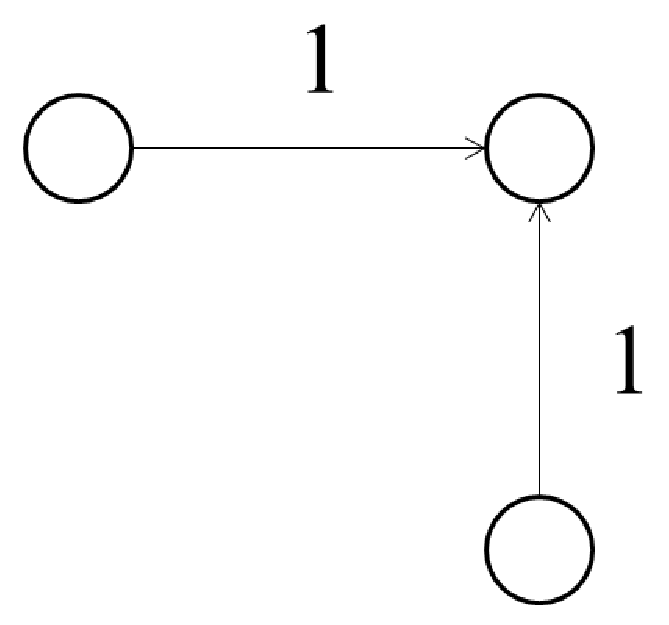
\includegraphics[height=2cm]{fig/path1.eps}
   &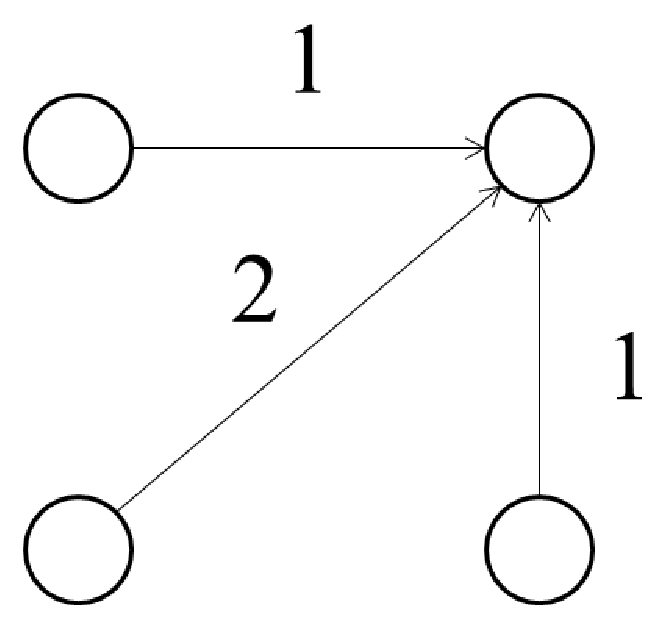
\includegraphics[height=2cm]{fig/path2.eps}
   &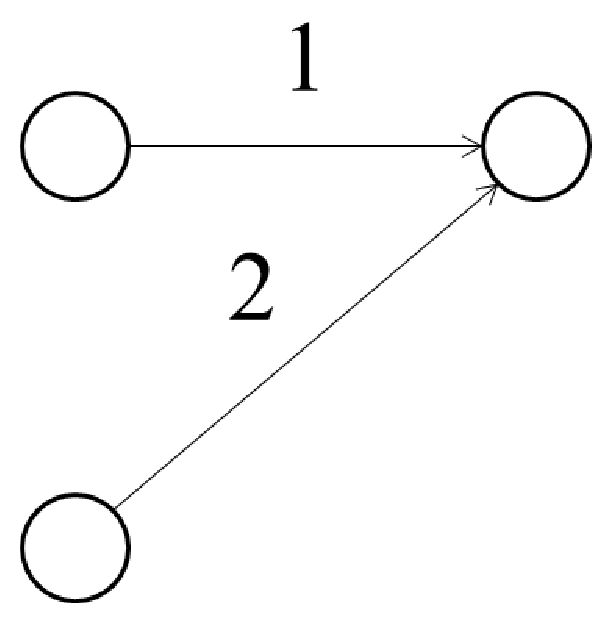
\includegraphics[height=2cm]{fig/path3.eps}\\
   &$P=1$&$P=2$&$P=3$\\
   &&&\\
   &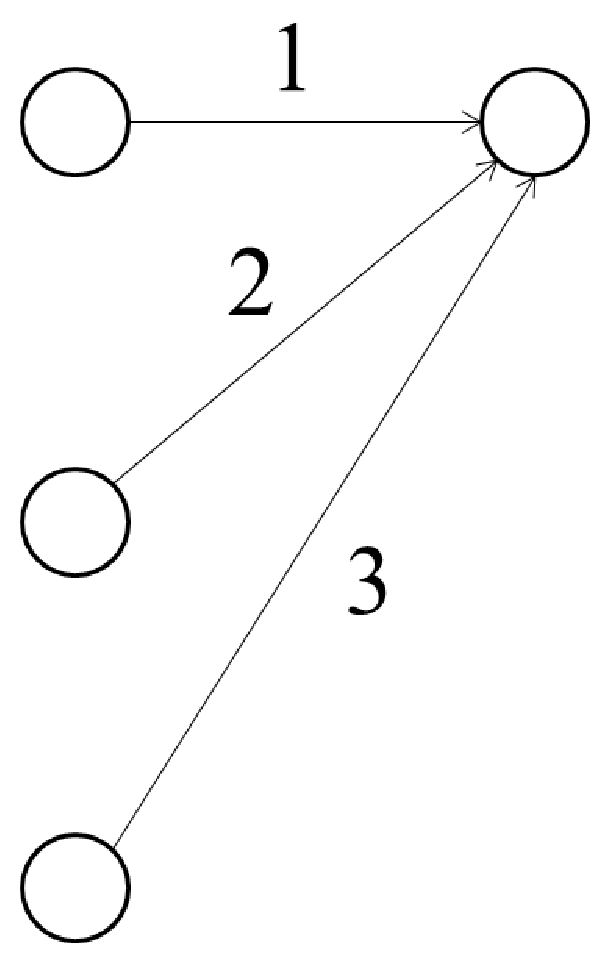
\includegraphics[height=3cm]{fig/path4.eps}
       &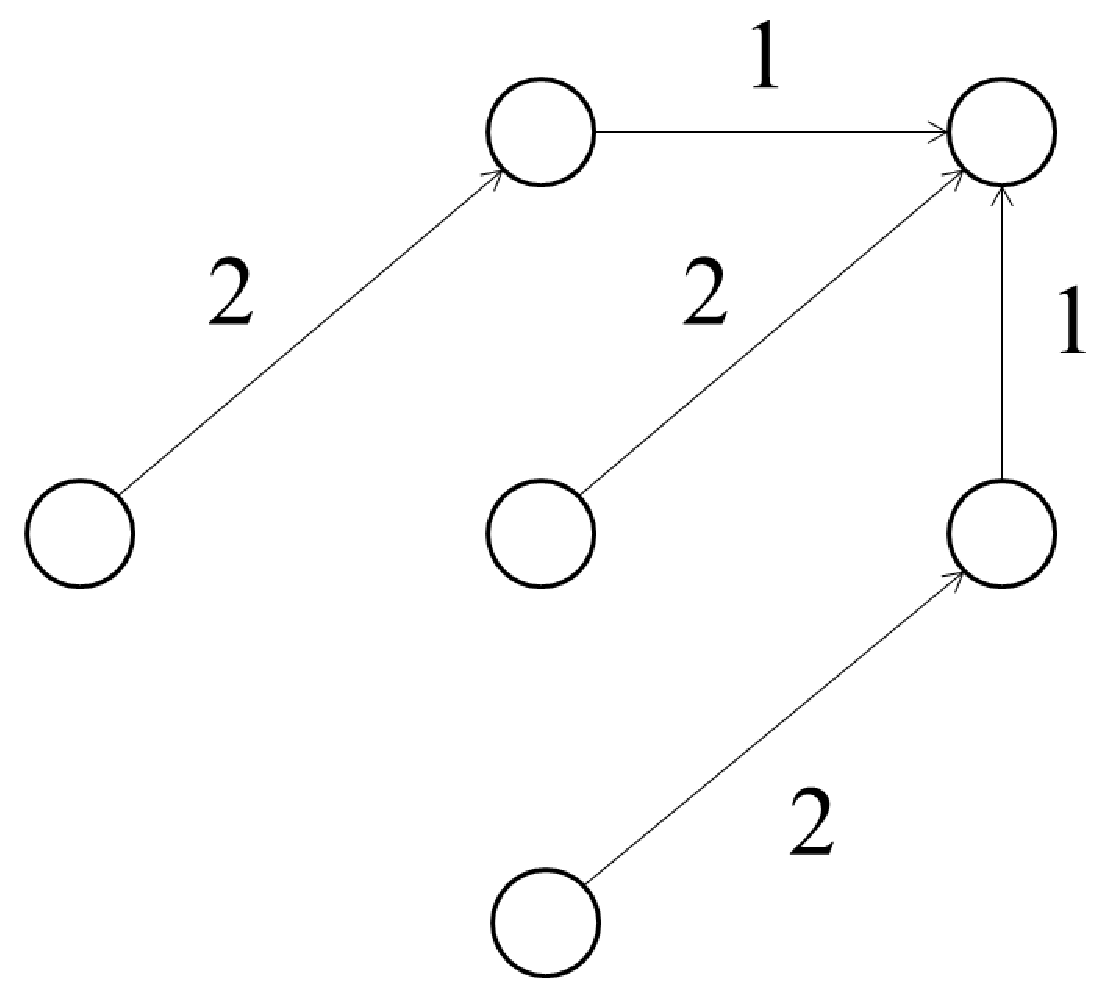
\includegraphics[height=3cm]{fig/path5.eps}
   &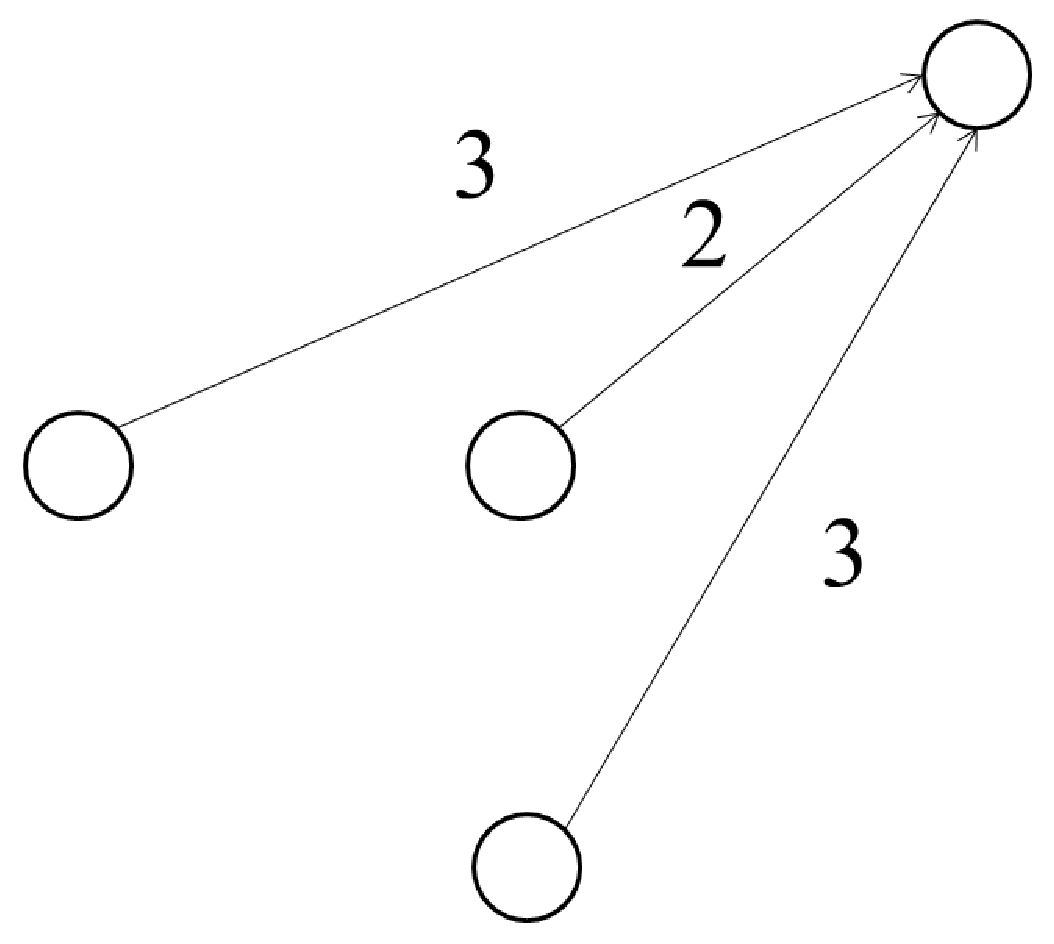
\includegraphics[height=3cm]{fig/path6.eps}\\
   &$P=4$&$P=5$&$P=6$\\
   &&&\\
   &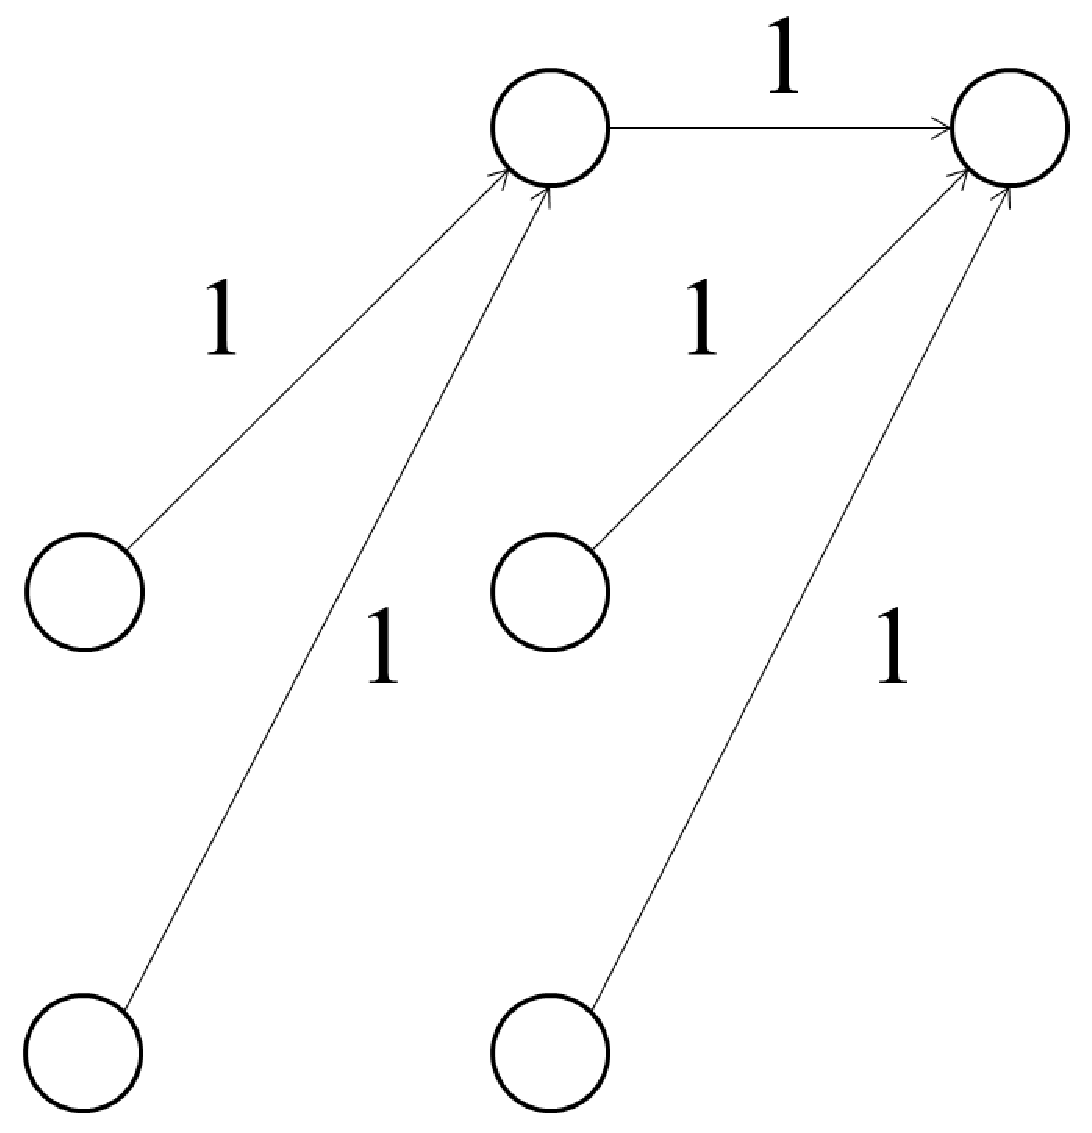
\includegraphics[height=3cm]{fig/path7.eps}
       &&\\
   &$P=7$&&\\
  \end{tabular}
 \end{center}
 \caption{candidates of local path constraint}
 \label{fig:dtw_cand}
\end{figure}

\begin{qsection}{SEE ALSO}
\hyperlink{vc}{vc}
\end{qsection}


\name{ds}{Sampling rate conversion (down sampling)}%
{sampling rate transformation}

\begin{synopsis}
\item[ds] [ --s $S$ ] [ {\em infile} ]
\end{synopsis}

\begin{qsection}{DESCRIPTION}
This command undertakes down sampling.
\par
Input and output data is in float format.
The following filter coefficient can be used.
\begin{tabular}{ll} \\[-1zh]
	$S=21$ & \$SPTK/lib/lpfcoef.2to1 \\
	$S=43$ & \$SPTK/lib/lpfcoef.4to3 \\
	$S=52,s=54$ & \$SPTK/lib/lpfcoef.5to2up \\
	& \$SPTK/lib/lpfcoef.5to2dn \\
        &(\$SPTK is the directory where toolkit was installed.)
\end{tabular}

Filter coefficients are in ascii formats.
\end{qsection}

\begin{options}
	\argm{s}{S}{conversion type\\
		\begin{tabular}{ll} \\[-1zh]
			$S=21$ & down sampling by $2:1$ \\
			$S=43$ & down sampling by $4:3$ \\
			$S=52$ & down sampling by $5:2$ \\
			$S=54$ & down sampling by $5:4$
		\end{tabular}\\\hspace*{\fill}}{21}
\end{options}

\begin{qsection}{EXAMPLE}
In this example, the speech data in the input file {\em data.16},
which was sampled at 16kHz in float format, is converted to
sampling rate of 8kHz:
\begin{quote}
\verb! ds data.16 > data.8 !
\end{quote}
\end{qsection}

%\begin{qsection}{SEE ALSO}
%
%\end{qsection}

\name{echo2}{$BI8=`%(%i!<$X$N=PNO(B}{$B$=$NB>(B}

\begin{synopsis}
\item[echo2] [ --n ] [ argument ]
\end{synopsis}

\begin{qsection}{DESCRIPTION}

{\em echo2} $B$O!$0z?t$rI8=`%(%i!<$K=PNO$7$^$9!%(B

\end{qsection}

\begin{options}
	\argm{n}{}{$B=PNO8e$K2~9T$7$^$;$s!%(B}{}
\end{options}

\begin{qsection}{EXAMPLE}
standard error$B$K2~9T$;$:$K!$(B''error!''$B$H=PNO$9$k!%(B
\begin{quote}
  \begin{verbatim}
  echo2 -n "error!"
  \end{verbatim}
\end{quote}
\end{qsection}

% ----------------------------------------------------------------- %
%             The Speech Signal Processing Toolkit (SPTK)           %
%             developed by SPTK Working Group                       %
%             http://sp-tk.sourceforge.net/                         %
% ----------------------------------------------------------------- %
%                                                                   %
%  Copyright (c) 1984-2007  Tokyo Institute of Technology           %
%                           Interdisciplinary Graduate School of    %
%                           Science and Engineering                 %
%                                                                   %
%                1996-2010  Nagoya Institute of Technology          %
%                           Department of Computer Science          %
%                                                                   %
% All rights reserved.                                              %
%                                                                   %
% Redistribution and use in source and binary forms, with or        %
% without modification, are permitted provided that the following   %
% conditions are met:                                               %
%                                                                   %
% - Redistributions of source code must retain the above copyright  %
%   notice, this list of conditions and the following disclaimer.   %
% - Redistributions in binary form must reproduce the above         %
%   copyright notice, this list of conditions and the following     %
%   disclaimer in the documentation and/or other materials provided %
%   with the distribution.                                          %
% - Neither the name of the SPTK working group nor the names of its %
%   contributors may be used to endorse or promote products derived %
%   from this software without specific prior written permission.   %
%                                                                   %
% THIS SOFTWARE IS PROVIDED BY THE COPYRIGHT HOLDERS AND            %
% CONTRIBUTORS "AS IS" AND ANY EXPRESS OR IMPLIED WARRANTIES,       %
% INCLUDING, BUT NOT LIMITED TO, THE IMPLIED WARRANTIES OF          %
% MERCHANTABILITY AND FITNESS FOR A PARTICULAR PURPOSE ARE          %
% DISCLAIMED. IN NO EVENT SHALL THE COPYRIGHT OWNER OR CONTRIBUTORS %
% BE LIABLE FOR ANY DIRECT, INDIRECT, INCIDENTAL, SPECIAL,          %
% EXEMPLARY, OR CONSEQUENTIAL DAMAGES (INCLUDING, BUT NOT LIMITED   %
% TO, PROCUREMENT OF SUBSTITUTE GOODS OR SERVICES; LOSS OF USE,     %
% DATA, OR PROFITS; OR BUSINESS INTERRUPTION) HOWEVER CAUSED AND ON %
% ANY THEORY OF LIABILITY, WHETHER IN CONTRACT, STRICT LIABILITY,   %
% OR TORT (INCLUDING NEGLIGENCE OR OTHERWISE) ARISING IN ANY WAY    %
% OUT OF THE USE OF THIS SOFTWARE, EVEN IF ADVISED OF THE           %
% POSSIBILITY OF SUCH DAMAGE.                                       %
% ----------------------------------------------------------------- %
\hypertarget{excite}{}
\name{excite}{generate excitation}{signal generation,speech analysis and synthesis}

\begin{synopsis}
\item [excite] [ --p $P$ ] [ --i $I$ ] [ --n ] [ --s $S$ ] [ {\em infile} ]
\end{synopsis}

\begin{qsection}{DESCRIPTION}
{\em excite} generates an excitation sequence 
from pitch period information from {\em infile} (or standard input), 
sending the result to standard output. 
When the pitch period is nonzero (i.e. voiced), 
the excitation sequence consists of a pulse train at that pitch. 
When the pitch period is zero (i.e. unvoiced),
the excitation sequence consists of Gaussian or M-sequence noise.

Input and output data are in float format.
\end{qsection}

\begin{options}
	\argm{p}{P}{frame period}{100}
	\argm{i}{I}{interpolation period}{1}
	\argm{n}{}{gauss/M-sequence for unvoiced\\
                   default is M-sequence}{FALSE}
	\argm{s}{S}{seed for nrand for Gaussian noise}{1}
\end{options}

\begin{qsection}{EXAMPLE}
In the example below, the excitation is generated from the
{\em data.p} file and passed through a LPC synthesis filter
whose coefficients are in the {\em data.lpc} file.
The speech signal is output to the {\em data.syn} file.
\begin{quote}
 \verb!excite < data.p | poledf data.lpc > data.syn!
\end{quote} 
In case we use Gaussian noise to generate are an unvoiced sound:
\begin{quote}
 \verb!excite -n < data.p | poledf data.lpc > data.syn!
\end{quote}
\end{qsection}

\begin{qsection}{SEE ALSO}
\hyperlink{poledf}{poledf}
\end{qsection}

\name{extract}{$B$"$k%$%s%G%C%/%9$KJ,N`$5$l$?F~NO%Y%/%H%k$NCj=P(B}%
{$B%Y%/%H%kNL;R2=(B}

\begin{synopsis}
\item [extract] [ --l $L$ ] [ --i $I$ ]  {\em indexfile}  [ {\em infile} ] 
\end{synopsis}

\begin{qsection}{DESCRIPTION}
 {\em extract}$B$O(B infile $B$+$i(B index $I$ $B$KJ,N`$5$l$?F~NO%Y%/%H%k$r(B
$BI8=`=PNO$K=PNO$7$^$9!%(B

\end{qsection}

\begin{options}
	\argm{l}{L}{$B%Y%/%H%k$N<!?t!%(B}{10}
	\argm{i}{I}{$B%3!<%I%V%C%/%$%s%G%C%/%9!%(B}{0}
\end{options}

\begin{qsection}{EXAMPLE}
float$B7A<0$N(B10$B<!$N%Y%/%H%k$N%U%!%$%k(B{\em data.v}$B$r%Y%/%H%kNL;R2=$7$?(B
$B7k2L$G$"$k(B{\em data.idx}$BCf$G(B
index $B$,(B 0 $B$H$J$k%Y%/%H%k$rCj=P$7!$(B{\em data.ex}$B$K=PNO$9$k(B:
\begin{quote}
\verb!extract -i 0 data.idx data.v > data.ex!
\end{quote}
\end{qsection}

\begin{qsection}{SEE ALSO}
ivq, vq
\end{qsection}

\name{fd}{$B%P%$%J%j%G!<%?$N%@%s%W(B}{$B%G!<%?A`:n(B}

\begin{synopsis}
 \item [fd] [ --a $A$ ] [ --n $N$ ] [ --m $M$ ] [ --{\em ent} ] 
	    [ +{\em type} ] [ $\%${\em form} ] [ {\em infile} ]
\end{synopsis}

\begin{qsection}{DESCRIPTION}
$B;XDj$5$l$?%U%!%$%k$NA4%G!<%?$r!$;XDj$5$l$?%U%)!<%^%C%H$G%@%s%W$7$^$9!%(B
$B%U%!%$%k$,;XDj$5$l$J$+$C$?>l9g!$%G!<%?$OI8=`F~NO$+$iFI$_9~$^$l$^$9!%(B
\end{qsection}

\begin{options}
	\argm{a}{A}{$B%"%I%l%9$D$-$G=PNO!%(B $A$ $B$O:G=i$N%"%I%l%9!%(B}{0}
	\argm{n}{N}{$BHV9fIU$-$G=PNO!%(B $N$ $B$O:G=i$NHV9f!%(B}{0}
	\argm{m}{M}{$BHV9fIU$1$r9T$J$&>l9g$K(B $M$ $B$K$h$k(B modulo $B$r$H$k!%(B}{EOF}
	\argm{{\em ent}}{}{{\em ent}$B$O?t;z$G!$(B1$B9T$K=PNO$9$k%G!<%?$N8D?t!%(B}{0}
	\argp{t}{$BF~NO%G!<%?$N7A<0!%(B \\
		\begin{tabular}{llcll} \\[-1zh]
			c & char$B7?(B (1byte) & \quad &
			s & short$B7?(B (2bytes) \\
			i & int$B7?(B (4bytes) & \quad &
			l & long$B7?(B (4bytes) \\
			f & float$B7?(B (4bytes) & \quad &
			d & double$B7?(B (8bytes) 
		\end{tabular}\\\hspace*{\fill}}{c}
        \argh{form}{}{$B=PNO$N%U%)!<%^%C%H;XDj!%(B\\
			C$B8@8l$N(Bprintf$B4X?t$N0z?t$N7A$G=PNO$N%U%)!<%^%C%H$r(B
			$B;XDj$9$k!%$?$@$7!$F~NO%G!<%?$N7A<0$,(Bf,d
                        $B$N;~$N$_M-8z!%(B}{N/A}
\end{options}

\begin{qsection}{EXAMPLE}
 $B2;@<%G!<%?(B sample.wav $B$r%"%I%l%9IU$-$G%@%s%W$9$k!%(B
\begin{quote}
 \verb!fd -a 0 sample.wav!
\end{quote}
 $B7k2L(B\\
\verb!000000  52 49 46 46 9a 15 00 00 57 41 56 45 66 6d 74 20 |RIFF....WAVEfmt |!\\
\verb!000010  10 00 00 00 01 00 01 00 40 1f 00 00 40 1f 00 00 |........@...@...|!\\
\verb!000020  01 00 08 00 64 61 74 61 76 15 00 00 8a 8a 8f 99 |....datav.......|!

\begin{center}
 $\vdots$\\
\end{center}
\end{qsection}

\begin{qsection}{SEE ALSO}
 dmp
\end{qsection}

% ----------------------------------------------------------------- %
%             The Speech Signal Processing Toolkit (SPTK)           %
%             developed by SPTK Working Group                       %
%             http://sp-tk.sourceforge.net/                         %
% ----------------------------------------------------------------- %
%                                                                   %
%  Copyright (c) 1984-2007  Tokyo Institute of Technology           %
%                           Interdisciplinary Graduate School of    %
%                           Science and Engineering                 %
%                                                                   %
%                1996-2013  Nagoya Institute of Technology          %
%                           Department of Computer Science          %
%                                                                   %
% All rights reserved.                                              %
%                                                                   %
% Redistribution and use in source and binary forms, with or        %
% without modification, are permitted provided that the following   %
% conditions are met:                                               %
%                                                                   %
% - Redistributions of source code must retain the above copyright  %
%   notice, this list of conditions and the following disclaimer.   %
% - Redistributions in binary form must reproduce the above         %
%   copyright notice, this list of conditions and the following     %
%   disclaimer in the documentation and/or other materials provided %
%   with the distribution.                                          %
% - Neither the name of the SPTK working group nor the names of its %
%   contributors may be used to endorse or promote products derived %
%   from this software without specific prior written permission.   %
%                                                                   %
% THIS SOFTWARE IS PROVIDED BY THE COPYRIGHT HOLDERS AND            %
% CONTRIBUTORS "AS IS" AND ANY EXPRESS OR IMPLIED WARRANTIES,       %
% INCLUDING, BUT NOT LIMITED TO, THE IMPLIED WARRANTIES OF          %
% MERCHANTABILITY AND FITNESS FOR A PARTICULAR PURPOSE ARE          %
% DISCLAIMED. IN NO EVENT SHALL THE COPYRIGHT OWNER OR CONTRIBUTORS %
% BE LIABLE FOR ANY DIRECT, INDIRECT, INCIDENTAL, SPECIAL,          %
% EXEMPLARY, OR CONSEQUENTIAL DAMAGES (INCLUDING, BUT NOT LIMITED   %
% TO, PROCUREMENT OF SUBSTITUTE GOODS OR SERVICES; LOSS OF USE,     %
% DATA, OR PROFITS; OR BUSINESS INTERRUPTION) HOWEVER CAUSED AND ON %
% ANY THEORY OF LIABILITY, WHETHER IN CONTRACT, STRICT LIABILITY,   %
% OR TORT (INCLUDING NEGLIGENCE OR OTHERWISE) ARISING IN ANY WAY    %
% OUT OF THE USE OF THIS SOFTWARE, EVEN IF ADVISED OF THE           %
% POSSIBILITY OF SUCH DAMAGE.                                       %
% ----------------------------------------------------------------- %
\hypertarget{fdrw}{}
\name{fdrw}{draw a graph}{plotting graphs}

\begin{synopsis}
\item[fdrw] [ --F $F$ ] [ --R $R$ ] [ --W $W$ ] [ --H $H$ ] [ --o $xo \; yo$ ] 
            [ --g $G$ ] [ --m $M$ ]   
\item[\ ~~~~~] [ --l $L$ ] [ --p $P$ ] [ --j $J$ ] [ --n $N$ ] [ --t $T$ ] 
	       [ --y $ymin \; ymax$ ] [ --z $Z$ ] [ --b ]  
\item[\ ~~~~~] [ {\em infile} ]
\end{synopsis}

\begin{qsection}{DESCRIPTION}
{\em fdrw} converts float data from {\em infile} (or standard input) 
to a plot formatted according to the FP5301 protocol, 
and sends the result to standard output.
One can control the details of the plot layout by setting the options bellow:
\end{qsection}

\begin{options}
	\argm{F}{F}{factor}{1}
	\argm{R}{R}{rotation angle}{0}
	\argm{W}{W}{width of figure ($\times 100$ mm)}{1}
	\argm{H}{H}{height of figure ($\times 100$ mm)}{1}
	\argm{o}{xo \; yo}{origin in mm}{20 25}
	\argm{g}{G}{draw grid ($0 \sim 2$)
                    (see also \hyperlink{fig}{fig})}{1}
	\argm{m}{M}{line type ($1 \sim 5$)\\
	\hspace*{2mm}1:~solid~~2:~dotted~~3:~dot and dash~~4:~broken~~5:~dash}{0}
	\argm{l}{L}{line pitch}{0}
	\argm{p}{P}{pen number ($1 \sim 10$)}{1}
	\argm{j}{J}{join number ($0 \sim 2$)}{1}
	\argm{n}{N}{number of samples}{0}
	\argm{t}{T}{rotation of coordinate axis. When $T=-1$, the
                    reference point is on the top-left. When $T=1$
                    the reference point is on the bottom-right.}{0}
	\argm{y}{ymin \; ymax}{scaling factor for $y$ axis}{-1 1}
	\argm{z}{Z}{This option is used when data is written
                    recursively in the $y$ axis. The distance between
                    two graphs in the $y$ axis is given by $Z$.}{0}
	\argm{b}{}{bar graph mode}{FALSE}
	\desc[1ex]{The $x$ axis scaling is automatically done so that
                every point in the input file is plotted in equally
                spaced  interrals
                for the assigned width.
                When the {\bf --n} option is omitted and the number of
                input samples is below 5000, then the block size is made
                equal to the number of samples.
                When the number of samples is above 5000,
                then the block size is made equal to 5000.}
	\desc{When the {\bf --y} option is omitted,
		the input data minimum value is set to $ymin$
                and the maximum value is set to $ymax$.}
\end{options}

\begin{qsection}{EXAMPLE}
In the example below, the impulse response of a digital filter is
drawn on the X window environment:
\begin{quote}
  \verb!impulse | dfs -a 1 0.8 0.5 | fdrw -H 0.3 | xgr!
\end{quote}
The graph width is 10cm and its height is 3cm.
\par
The next example draws the magnitude of
the frequency response of a digital filter on the X window environment:
\begin{quote}
  \verb!impulse | dfs -a 1 0.8 0.5 | spec | fdrw -y -60 40 | xgr!
\end{quote}
The $y$ axis goes from $-60$ dB to $40$ dB.
\par
The running spectrum can be draw on the X window environment by:
\begin{quote}
 \verb!fig -g 0 -W 0.4 << EOF ! \\
 \verb!~~~~x 0 5 !\\
 \verb!~~~~xscale 0 1 2 3 4 5 !\\
 \verb!~~~~xname "FREQUENCY (kHz)"!\\
 \verb!EOF!\\
 \verb!spec < data |\ !\\
 \verb!fdrw -W 0.4 -H 0.2 -g 0 -n 129 -y -30 30 -z 3 |\ !\\
 \verb!xgr !
\end{quote}
The command {\em psgr} prints the output to a laser printer in the
same manner as it is printed on the screen.
Since the {\em fdrw} command includes a sequence of commands
for a plotter machine (FP5301 protocol) in the output file,
its output can be directly sent to a printer.
\end{qsection}

\begin{qsection}{SEE ALSO}
\hyperlink{fig}{fig},
\hyperlink{xgr}{xgr},
\hyperlink{psgr}{psgr}
\end{qsection}

\name{fft}{$B9bB.%U!<%j%(JQ49(B}

\begin{synopsis}
\item[fft] [ --l $L$ ] [ --m $M$] [ --\{ A $|$ R $|$ I $|$ P \} ] 
	   [ {\em infile} ] 
\end{synopsis}

\begin{qsection}{DESCRIPTION}
$BJ#AG7ONs$r(B{\em infile} $B$+$iFI$_9~$_!$(BFFT $B%"%k%4%j%:%`$K$h$j(BDFT $B$r<B9T$7$^$9!%(B
{\em infile} $B$N;XDj$,$J$$$H$-$K$O!$I8=`F~NO$+$i%G!<%?$,FI$_9~$^$l$^$9!%(B
$B%G!<%?7A<0$OF~=PNO$H$b(Bfloat $B7A$G!$F~=PNO%G!<%?$N=g=x$O<!$NDL$j$G$9!%(B
\[
 \begin{array}{lll}
\mbox{$BF~NO7ONs(B} & \overbrace{\framebox[4.5cm]{$B<B!!It(B}}^{M+1} &
	   \overbrace{\framebox[4.5cm]{$B5u!!It(B}}^{M+1} \\
		& \makebox[4.5cm]{0\hfill $M$} &
		\makebox[4.5cm]{0\hfill $M$}
\end{array}
\]
\[
\begin{array}{lll}
\mbox{$B=PNO7ONs(B} & \overbrace{\framebox[4.5cm]{$B<B!!It(B}}^{L} &
	   \overbrace{\framebox[4.5cm]{$B5u!!It(B}}^{L} \\
		& \makebox[4.5cm]{0\hfill $L-1$} &
		\makebox[4.5cm]{0\hfill $L-1$}
\end{array}
\]
\end{qsection}

\begin{options}
	\argm{l}{L}{$B%U!<%j%(JQ49$N%5%$%:!%(B2 $B$N$Y$->h$G;XDj!%(B}{256}
	\argm{m}{M}{$BJ#AG7ONs$N<!?t!%(B}{L-1}
	\argm{A}{}{$B?6I}%9%Z%/%H%k$r=PNO!%(B}{FALSE}
	\argm{R}{}{$B<BIt$N$_$r=PNO!%(B}{FALSE}
	\argm{I}{}{$B5uIt$N$_$r=PNO!%(B}{FALSE}
	\argm{P}{}{$B%Q%o!<%9%Z%/%H%k$r=PNO!%(B}{FALSE}
\end{options}

\begin{qsection}{EXAMPLE}
float$B7A<0$N%U%!%$%k(B {\em data.f} $B$K$"$kJ#AG?tNs!J<BIt(B256$BE@!$5uIt(B256$BE@!K$N(B DFT $B$N?6I}$r5a$a!$(B{\em data.dft} $B$K=PNO$9$k(B:
\begin{quote}
  \verb!fft data.f -l 256 -A > data.dft!
\end{quote}
\end{qsection}

%\begin{qsection}{BUGS}
% FFT $B$N%5%$%:$O(B1024 $B0J2<!%(B
%\end{qsection}

\begin{qsection}{SEE ALSO}
  fftr, spec, phase
\end{qsection}

% ----------------------------------------------------------------
%       Speech Signal Processing Toolkit (SPTK): version 3.0
%                      SPTK Working Group
% 
%                Department of Computer Science
%                Nagoya Institute of Technology
%                             and
%   Interdisciplinary Graduate School of Science and Engineering
%                Tokyo Institute of Technology
%                   Copyright (c) 1984-2000
%                     All Rights Reserved.
% 
% Permission is hereby granted, free of charge, to use and
% distribute this software and its documentation without
% restriction, including without limitation the rights to use,
% copy, modify, merge, publish, distribute, sublicense, and/or
% sell copies of this work, and to permit persons to whom this
% work is furnished to do so, subject to the following conditions:
% 
%   1. The code must retain the above copyright notice, this list
%      of conditions and the following disclaimer.
% 
%   2. Any modifications must be clearly marked as such.
%                                                                        
% NAGOYA INSTITUTE OF TECHNOLOGY, TOKYO INSITITUTE OF TECHNOLOGY,
% SPTK WORKING GROUP, AND THE CONTRIBUTORS TO THIS WORK DISCLAIM
% ALL WARRANTIES WITH REGARD TO THIS SOFTWARE, INCLUDING ALL
% IMPLIED WARRANTIES OF MERCHANTABILITY AND FITNESS, IN NO EVENT
% SHALL NAGOYA INSTITUTE OF TECHNOLOGY, TOKYO INSITITUTE OF
% TECHNOLOGY, SPTK WORKING GROUP, NOR THE CONTRIBUTORS BE LIABLE
% FOR ANY SPECIAL, INDIRECT OR CONSEQUENTIAL DAMAGES OR ANY
% DAMAGES WHATSOEVER RESULTING FROM LOSS OF USE, DATA OR PROFITS,
% WHETHER IN AN ACTION OF CONTRACT, NEGLIGENCE OR OTHER TORTIOUS
% ACTION, ARISING OUT OF OR IN CONNECTION WITH THE USE OR
% PERFORMANCE OF THIS SOFTWARE.
% ----------------------------------------------------------------
%
\name{fft2}{ʣ�ǿ����2������®�ա��ꥨ�Ѵ�}{�������}

\begin{synopsis}
\item[fft2] [ --l $L$ ] [ --m $M_1 \; M_2$ ] [ --t ] [ --c ] [ --q ] 
            [ --\{ A $|$ R $|$ I $|$ P \} ]  
\item[\ ~~~~] [ {\em infile} ]  
\end{synopsis}

\begin{qsection}{DESCRIPTION}

{\em fft2} �ϡ�ʣ�ǿ���Ϳ������ǡ������{\em infile}�����ɤ߹����2����
�ա��ꥨ�Ѵ���Ԥʤ�����̤�ɸ����Ϥ˽��Ϥ��ޤ���
�����ϤΥǡ����ե����ޥåȤϰʲ����̤�Ǥ���
\begin{center}
\leavevmode
\includegraphics{fig/fft2.eps}
\end{center}
\end{qsection}

\begin{options}
	\argm{l}{L}{�ա��ꥨ�Ѵ��Υ������� 2 �Τ٤���ǻ��ꡥ}{64}
	\argm{m}{M_1 \; M_2}{�ǡ����μ����� $M_1\times M_2$ �ǻ��ꡥ
			�ե����륵���� $k$ �� $64^2\times 2$ ���⾮������硤
			$\sqrt{k\div 2}$ �������ʤ�� $M_1=M_2=\sqrt{k\div 2}$ 
			�Ȥ��������Ǥʤ�����ɸ�२�顼���Ϥ˥��顼��å�����
			����Ϥ��Ƥ��������λ��}{$64 , M_1$}
	\argm{t}{}{FFT�η�̤�transpose���ƽ��ϡ�
		\begin{center}
		\leavevmode
		\includegraphics{fig/fft2-trans.eps}
		\end{center}~}{FALSE}
	\argm{c}{}{transpose����ݡ�������1�ǡ�����ȿ��¦������äƤ��ơ�
		   $(L+1)\times (L+1)$�ĤΥǡ�������ϡ�
		\begin{center}	
		\leavevmode
		\includegraphics{fig/fft2-comp.eps}
		\end{center}~}{FALSE}
	\argm{q}{}{FFT�η�̤κǽ��1/4�Υǡ����Τߤ���ϡ� 
		   ���κ�c���ץ�����Ʊ�ͤ˶����������Ԥʤ���
		   $(\frac{L}{2}+1)\times(\frac{L}{2}+1)$ �ĤΥǡ�������ϡ�
		\begin{center}
		\leavevmode
		\includegraphics{fig/fft2-quad.eps}
		\end{center}~}{FALSE} %\hspace*{\fill}
	\argm{A}{}{�������ڥ��ȥ����ϡ�}{FALSE}
	\argm{R}{}{�����Τߤ���ϡ�}{FALSE}
	\argm{I}{}{�����Τߤ���ϡ�}{FALSE}
	\argm{P}{}{�ѥ���ڥ��ȥ����ϡ�}{FALSE}
\end{options}

\begin{qsection}{EXAMPLE}
float�����Υե�����{\em data.f} �ˤ���2����ʣ�ǿ���� DFT �ο������ᡤ
{\em data.dft} �˽��Ϥ���:
\begin{quote}
  \verb!fft2 -A data.f > data.dft!
\end{quote}
\end{qsection}

\begin{qsection}{SEE ALSO}
 fft, fftr2, ifft
\end{qsection}

% ----------------------------------------------------------------
%       Speech Signal Processing Toolkit (SPTK): version 3.0
%                      SPTK Working Group
% 
%                Department of Computer Science
%                Nagoya Institute of Technology
%                             and
%   Interdisciplinary Graduate School of Science and Engineering
%                Tokyo Institute of Technology
%                   Copyright (c) 1984-2000
%                     All Rights Reserved.
% 
% Permission is hereby granted, free of charge, to use and
% distribute this software and its documentation without
% restriction, including without limitation the rights to use,
% copy, modify, merge, publish, distribute, sublicense, and/or
% sell copies of this work, and to permit persons to whom this
% work is furnished to do so, subject to the following conditions:
% 
%   1. The code must retain the above copyright notice, this list
%      of conditions and the following disclaimer.
% 
%   2. Any modifications must be clearly marked as such.
%                                                                        
% NAGOYA INSTITUTE OF TECHNOLOGY, TOKYO INSITITUTE OF TECHNOLOGY,
% SPTK WORKING GROUP, AND THE CONTRIBUTORS TO THIS WORK DISCLAIM
% ALL WARRANTIES WITH REGARD TO THIS SOFTWARE, INCLUDING ALL
% IMPLIED WARRANTIES OF MERCHANTABILITY AND FITNESS, IN NO EVENT
% SHALL NAGOYA INSTITUTE OF TECHNOLOGY, TOKYO INSITITUTE OF
% TECHNOLOGY, SPTK WORKING GROUP, NOR THE CONTRIBUTORS BE LIABLE
% FOR ANY SPECIAL, INDIRECT OR CONSEQUENTIAL DAMAGES OR ANY
% DAMAGES WHATSOEVER RESULTING FROM LOSS OF USE, DATA OR PROFITS,
% WHETHER IN AN ACTION OF CONTRACT, NEGLIGENCE OR OTHER TORTIOUS
% ACTION, ARISING OUT OF OR IN CONNECTION WITH THE USE OR
% PERFORMANCE OF THIS SOFTWARE.
% ----------------------------------------------------------------
%
\name{fftcep}{FFT$B%1%W%9%H%i%`(B}{$B?.9f=hM}(B}

\begin{synopsis}
\item[fftcep] [ --m $M$ ] [ --l $L$ ] [ --j $J$ ] [ --k $K$ ] 
	    [ --e $E$ ] [ {\em infile} ] 
\end{synopsis}

\begin{qsection}{DESCRIPTION}
FFT$B%1%W%9%H%i%`78?t(B $c(m)$ $B$r(B
$BI8=`=PNO$K=PNO$7$^$9!%(B
$BF~NO$OAk3]$1$5$l$?D9$5(B $L$ $B$N;~7ONs(B
\begin{displaymath}
  x(0),x(1),\ldots,x(L-1)
\end{displaymath}
$B$G$9!%(B
\par
$B%G!<%?7A<0$OF~NO!$=PNO$H$b(Bfloat $B7A<0$G$9!%(B
\par
%$B=>Mh$N%1%W%9%H%i%`K!$G$O!$%1%W%9%H%i%`$NDc%1%U%l%s%7!<@.J,(B
%$B$r<h$j=P$9$3$H$GJ?3j2=%9%Z%/%H%k$r5a$a$F$$$^$7$?!%(B
%$B$7$+$7!$$3$NJ}K!$G$O%9%Z%/%H%k$NHy:Y9=B$$N1F6A$r==J,<h$j=|$$$F$$$k$H$O$$$($:!$(B
%$BF@$i$l$k%9%Z%/%H%kJqMm$,%U%l!<%`Kh$KMp$l$k$H$$$&7gE@$,$"$j$^$7$?!%(B
\par
%$B$3$l$KBP$7$F!$2~NI%1%W%9%H%i%`K!$O!$%9%Z%/%H%k$NHy:Y9=B$$rDL$kJqMm$r??$NJqMm$H(B
%$B9M$(!$%9%Z%/%H%k$HJ?3j2=%9%Z%/%H%k$N:9J,$KBP$7$F$5$i$KJ?3j2=$r7+$jJV$9$3$H$K(B
%$B$h$j!$??$NJqMm$rCj=P$7$h$&$H$9$k<jK!$G$9!%(B
$B7+$jJV$72s?t(B$J$$B$*$h$S!"2CB.78?t(B$K$$B$r;XDj$7$?>l9g!$(B
$B2~NI%1%W%9%H%i%`K!$K$h$j%1%W%9%H%i%`78?t$r7W;;$7$^$9!%(B
\end{qsection}

\begin{options}
	\argm{m}{M}{$BJ,@O<!?t!%(B}{25}
	\argm{l}{L}{$B%U%l!<%`D9!%(B}{256}
	\argm{j}{J}{$B7+$jJV$72s?t!%(B}{0}
	\argm{k}{K}{$B2CB.78?t!%(B}{0.0}
	\argm{e}{E}{$B?6I}%9%Z%/%H%k$NBP?t$r$H$k:]$KB-$79~$`>.$5$JCM!%(B}{0.0}
\end{options}

\begin{qsection}{EXAMPLE}
float $B7A<0$N2;@<%G!<%?(B {\em data.f} $B$rJ,@O$7!$(B{\em data.cep}
 $B$K%1%W%9%H%i%`78?t$rF@$k(B:
\begin{quote}
  \verb!frame < data.f | window | fftcep > data.cep !
\end{quote}
\end{qsection}

\begin{qsection}{SEE ALSO}
  uels, ceps
\end{qsection}

% ----------------------------------------------------------------- %
%             The Speech Signal Processing Toolkit (SPTK)           %
%             developed by SPTK Working Group                       %
%             http://sp-tk.sourceforge.net/                         %
% ----------------------------------------------------------------- %
%                                                                   %
%  Copyright (c) 1984-2007  Tokyo Institute of Technology           %
%                           Interdisciplinary Graduate School of    %
%                           Science and Engineering                 %
%                                                                   %
%                1996-2011  Nagoya Institute of Technology          %
%                           Department of Computer Science          %
%                                                                   %
% All rights reserved.                                              %
%                                                                   %
% Redistribution and use in source and binary forms, with or        %
% without modification, are permitted provided that the following   %
% conditions are met:                                               %
%                                                                   %
% - Redistributions of source code must retain the above copyright  %
%   notice, this list of conditions and the following disclaimer.   %
% - Redistributions in binary form must reproduce the above         %
%   copyright notice, this list of conditions and the following     %
%   disclaimer in the documentation and/or other materials provided %
%   with the distribution.                                          %
% - Neither the name of the SPTK working group nor the names of its %
%   contributors may be used to endorse or promote products derived %
%   from this software without specific prior written permission.   %
%                                                                   %
% THIS SOFTWARE IS PROVIDED BY THE COPYRIGHT HOLDERS AND            %
% CONTRIBUTORS "AS IS" AND ANY EXPRESS OR IMPLIED WARRANTIES,       %
% INCLUDING, BUT NOT LIMITED TO, THE IMPLIED WARRANTIES OF          %
% MERCHANTABILITY AND FITNESS FOR A PARTICULAR PURPOSE ARE          %
% DISCLAIMED. IN NO EVENT SHALL THE COPYRIGHT OWNER OR CONTRIBUTORS %
% BE LIABLE FOR ANY DIRECT, INDIRECT, INCIDENTAL, SPECIAL,          %
% EXEMPLARY, OR CONSEQUENTIAL DAMAGES (INCLUDING, BUT NOT LIMITED   %
% TO, PROCUREMENT OF SUBSTITUTE GOODS OR SERVICES; LOSS OF USE,     %
% DATA, OR PROFITS; OR BUSINESS INTERRUPTION) HOWEVER CAUSED AND ON %
% ANY THEORY OF LIABILITY, WHETHER IN CONTRACT, STRICT LIABILITY,   %
% OR TORT (INCLUDING NEGLIGENCE OR OTHERWISE) ARISING IN ANY WAY    %
% OUT OF THE USE OF THIS SOFTWARE, EVEN IF ADVISED OF THE           %
% POSSIBILITY OF SUCH DAMAGE.                                       %
% ----------------------------------------------------------------- %
\hypertarget{fftr}{}
\name{fftr}{FFT for real sequence}{signal processing}

\begin{synopsis}
 \item[fftr] [ --l $L$ ] [ --m $M$] [ --\{ A $|$ R $|$ I $|$ P \} ] [ --H ]
             [ {\em infile} ] 
\end{synopsis}

\begin{qsection}{DESCRIPTION}
{\em fftr} uses the Fast Fourier Transform (FFT) algorithm 
to calculate the Discrete Fourier Transform (DFT) 
of real-valued input data in {\em infile} (or standard input), 
and sends the result to standard output. 
When the --m option is omitted 
and the input data sequence length is less than the FFT size, 
the input data is padded with zeros.
The input and output data is in float format, 
arranged as below.
\begin{displaymath}
\begin{array}{lll}
\mbox{Input sequence} & 
\overbrace{\framebox[4.5cm]{$x_0, x_1, \ldots, x_{M}, 0,
                                        \ldots,0$}}^{L}  & \\
                & \makebox[4.5cm]{0\hfill $L-1$} &
\end{array}
\end{displaymath}
\begin{displaymath}
\begin{array}{lll}
\mbox{Output sequence} & \overbrace{\framebox[4.5cm]{real part}}^{L} &
           \overbrace{\framebox[4.5cm]{imaginary part}}^{L} \\
                & \makebox[4.5cm]{0\hfill $L-1$} &
                \makebox[4.5cm]{0\hfill $L-1$}
\end{array}
\end{displaymath}
\end{qsection}

\begin{options}
        \argm{l}{L}{FFT size power of 2}{256}
        \argm{m}{M}{order of sequence}{L-1}
        \argm{A}{}{output magnitude}{FALSE}
        \argm{R}{}{output real part}{FALSE}
        \argm{I}{}{output imaginary part}{FALSE}
        \argm{P}{}{output power spectrum}{FALSE}
        \argm{H}{}{output half size}{FALSE}
\end{options}

\begin{qsection}{EXAMPLE}
In the example below, a sine wave is passed through a Blackman window,
its DFT is evaluated and the magnitude is plotted:
\begin{quote}
  \verb!sin -p 30 | window | fftr -A | fdrw | xgr!
\end{quote}

\end{qsection}

\begin{qsection}{SEE ALSO}
\hyperlink{fft}{fft},
\hyperlink{spec}{spec},
\hyperlink{phase}{phase}
\end{qsection}

% ----------------------------------------------------------------
%       Speech Signal Processing Toolkit (SPTK): version 3.0
%                      SPTK Working Group
% 
%                Department of Computer Science
%                Nagoya Institute of Technology
%                             and
%   Interdisciplinary Graduate School of Science and Engineering
%                Tokyo Institute of Technology
%                   Copyright (c) 1984-2000
%                     All Rights Reserved.
% 
% Permission is hereby granted, free of charge, to use and
% distribute this software and its documentation without
% restriction, including without limitation the rights to use,
% copy, modify, merge, publish, distribute, sublicense, and/or
% sell copies of this work, and to permit persons to whom this
% work is furnished to do so, subject to the following conditions:
% 
%   1. The code must retain the above copyright notice, this list
%      of conditions and the following disclaimer.
% 
%   2. Any modifications must be clearly marked as such.
%                                                                        
% NAGOYA INSTITUTE OF TECHNOLOGY, TOKYO INSITITUTE OF TECHNOLOGY,
% SPTK WORKING GROUP, AND THE CONTRIBUTORS TO THIS WORK DISCLAIM
% ALL WARRANTIES WITH REGARD TO THIS SOFTWARE, INCLUDING ALL
% IMPLIED WARRANTIES OF MERCHANTABILITY AND FITNESS, IN NO EVENT
% SHALL NAGOYA INSTITUTE OF TECHNOLOGY, TOKYO INSITITUTE OF
% TECHNOLOGY, SPTK WORKING GROUP, NOR THE CONTRIBUTORS BE LIABLE
% FOR ANY SPECIAL, INDIRECT OR CONSEQUENTIAL DAMAGES OR ANY
% DAMAGES WHATSOEVER RESULTING FROM LOSS OF USE, DATA OR PROFITS,
% WHETHER IN AN ACTION OF CONTRACT, NEGLIGENCE OR OTHER TORTIOUS
% ACTION, ARISING OUT OF OR IN CONNECTION WITH THE USE OR
% PERFORMANCE OF THIS SOFTWARE.
% ----------------------------------------------------------------
%
\hypertarget{fftr2}{}
\name{fftr2}{2-dimensional FFT for real sequence}{signal processing}

\begin{synopsis}
\item[fftr2] [ --l $L$ ] [ --m $M_1 \; M_2$ ] [ --t ] [ --c ] [ --q ] 
	     [ --\{ A $|$ R $|$ I $|$ P \} ] [ {\em infile} ] 
\end{synopsis}

\begin{qsection}{DESCRIPTION}
{\em fftr2} uses the 2-dimensional Fast Fourier Transform (FFT) algorithm 
to calculate the 2-dimensional Discrete Fourier Transform (DFT) 
of real-valued input data from {\em infile} (or standard input), 
sending the result to standard output. 
The input and output data is in float format, arranged as follows.
\begin{center}
 \leavevmode
 \includegraphics{fig/fftr2.eps}
\end{center}
\end{qsection}

\begin{options}
	\argm{l}{L}{FFT size  power of 2}{64}
	\argm{m}{M_1 \; M_2}{order of sequence ($M_1\times M_2$).
			If the file size $k$ is smaller than $64^2$
			and $\sqrt{k}$ is integer value, $M_1=M_2=\sqrt{k}$. 
			Otherwise output error message to standard error output 
			and then terminate.}{$64 , M_1$}
	\argm{t}{}{Output results in transposed form (see also \hyperlink{fft2}{fft2}).}{FALSE}
	\argm{c}{}{When results are transposed, 1 boundary data is copied from the
	opposite side, and then output $(L+1)\times (L+1)$ data (see also \hyperlink{fft2}{fft2}).}{FALSE}
	\argm{q}{}{Output first $1/4$ data of FFT results only.
		   As in the above c option, boundary data is compensated and 
		   $(\frac{L}{2}+1)\times(\frac{L}{2}+1)$ data are output
		   (see also \hyperlink{fft2}{fft2}).}{FALSE}
	\argm{A}{}{amplitude}{FALSE}
	\argm{R}{}{real part}{FALSE}
	\argm{I}{}{imaginary part}{FALSE}
	\argm{P}{}{output power spectrum}{FALSE}
\end{options}

\begin{qsection}{EXAMPLE}
This example reads a sequence of 2-dimensional real numbers in float format
from {\em data.f} file, evaluates its 2-dimensional DFT and outputs results to {\em
data.dft} file:
\begin{quote}
  \verb!fftr2 -A data.f > data.dft!
\end{quote}
\end{qsection}

\begin{qsection}{SEE ALSO}
\hyperlink{fft}{fft},
\hyperlink{fft2}{fft2},
\hyperlink{ifft}{ifft}
\end{qsection}
 
\name{fig}{$B?^$r:n@.$9$k(B}
\begin{synopsis}
 \item[fig] [ --F $F$ ] [ --R $R$ ] [ --W $W$ ] [ --H $H$] [ --o $xo$ $yo$ ]
	    [ --g $G$ ]  [ --p $P$ ] 
 \item[\ ~~~] [ --s $S$ ] [ --f $file$ ] [ --t ] [ {\em infile} ]
\end{synopsis}

\begin{qsection}{DESCRIPTION}
$B%U%!%$%k(B {\em infile} ($B>JN,;~$OI8=`F~NO(B)$B$+$iM?$($i$l$k%3%^%s%I$K$h$j%0%i%U$r(B
$BIA$-$^$9!%(B
UNIX$BI8=`%3%^%s%I$N(B graph $B$HF1MM$J5!G=$,$"$kB>!$%0%i%U$N:BI8<4!$L\@9$j!$L>A0$r(B
$BF~$l$k5!G=$,$"$j$^$9!%=PNO$O%W%m%C%?$N%3%^%s%INs$G$9!%$=$N$?$a!$(BX$BC<Kv$K=PNO(B
$B$9$k>l9g$O%3%^%s%I(B xgr$B!$%]%9%H%9%/%j%W%H$K=PNO$9$k>l9g$O%3%^%s%I(Bpsgr$B$r;HMQ(B
$B$7$F2<$5$$!%(B
\end{qsection}

\begin{options}
	\argm{F}{F}{$B%0%i%U$rIA$/G\N(!%(B}{1}
	\argm{R}{R}{$B%0%i%U$rIA$/3QEY!%(B}{0}
	\argm{W}{W}{$B%0%i%U$NI}(B($\times 100$mm)$B!%(B}{1}
	\argm{H}{H}{$B%0%i%U$N9b$5(B($\times 100$mm)$B!%(B}{1}
	\argm{o}{xo \; yo}{$B%0%i%U$rIA$/0LCV!%(B $BIA2h0h$N:82<$r86E@$H$7$F!$(B
			   $B%0%i%U$N:82<$N0LCV$r(Bmm $B$G;XDj!%(B}{20 20}
	\argm{g}{G}{$B%0%i%U$NOH$N7A<0(B($0 \sim 2$)$B!%(B\\
			\begin{tabular}{cccc}
			&\epsfxsize=2cm \epsffile{fig/g0.eps}
			&\epsfxsize=2cm \epsffile{fig/g1.eps}
			&\epsfxsize=2cm \epsffile{fig/g2.eps}\\
			$G$&0&1&2	 
			\end{tabular}\\\hspace*{\fill}}{2}
	\argm{p}{P}{$B%Z%sHV9f(B($1 \sim 10$)$B!%(B}{1}
	\argm{s}{S}{$BJ8;z%5%$%:(B($1 \sim 4$)$B!%(B}{1}
	\argm{f}{file}{$B%3%^%s%I<B9T;~!$:G=i$KFI$_9~$`%U%!%$%k!%(B
		       ($infile$ $B$h$jM%@h(B)$B!%(B}{NULL}
	\argm{t}{}{ $x$ $B<4$H(B $y$ $B<4$rF~$l49$($k!%(B}{FALSE}
\end{options}

\begin{qsection}{EXAMPLE}
{\em data.fig} $B$N%0%i%U$r(BX$BC<Kv$K=PNO$9$k!%(B
\vspace{-3mm}
\begin{quote}
 \verb!fig data.fig |xgr!
\end{quote}
\vspace{-3mm}
{\em data.fig} $B$N%0%i%U$r%]%9%H%9%/%j%W%H$K$7$?%G!<%?$r(Bghostview$B$G8+$k!%(B
\vspace{-3mm}
\begin{quote}
 \verb!fig data.fig | psgr | ghostview -!
\end{quote}
\vspace{-3mm}
\end{qsection}

\vspace{-1cm}
\begin{qsection}{USAGE}
$B!!(B\vspace{-1cm}
\end{qsection}

\begin{qsection}{\ ~~~$B%3%^%s%I(B}
$BF~NO%G!<%?$O%3%^%s%I9T$H%G!<%?9T$K$o$1$k$3$H$,$G$-$^$9!%(B
$B%3%^%s%I9T$O!$%0%i%U$NL\@9$j!$L>A0!$%9%1!<%j%s%0Ey$r;XDj$7$^$9!%(B
$B%G!<%?9T$O(B($x ~y$)$B:BI8%Z%"$r;XDj$7$^$9!%(B
$B%3%^%s%I9T$K$h$C$F;XDj$5$l$??tCM$O!$<!$N%3%^%s%I9T$K$h$k@_Dj$,$J$5$l$k$^$G(B
$BM-8z$G$9!%(B\\
\end{qsection}

\vspace{-1cm}
\begin{qsection}{\ ~~~$B%3%^%s%I9T(B}
\begin{minipage}[t]{5.5cm}
x [mel $\alpha$]~ $xmin$ ~$ymax$ [$xa$]\\
y [mel $\alpha$]~ $xmin$ ~$ymax$ [$ya$]\\
\end{minipage}
\begin{minipage}[t]{9cm}
 $x$ $B<4!$(B $y$ $B<4$N%9%1!<%j%s%0$r@_Dj$7$^$9!%(B\\
$xa$$B!$(B$ya$ $B$OL\@9$j$rBG$D<4$N0LCV$r;XDj$7$^$9!%(B
$B>JN,$5$l$?>l9g!$(B $xa = xmin$ $B!$(B $ya = ymin$ $B$H$J$j$^$9!%(B\\
mel $\alpha$ ($\alpha$ $B$O?t;z$G!$(B $BNc$($P(B mel 0.35) $B$r;XDj$9$k$H!$(B
1$B<!%*!<%k%Q%9%U%#%k%?$N0LAjFC@-$K$h$j<~GH?tJQ49$7$?L\@9$j$H$_$J$7$^$9!%(B
\end{minipage} \\

\begin{minipage}[t]{5.5cm}
xscale ~$x_1$ $x_2$ $x_3$ $\cdots$\\
yscale ~$y_1$ $y_2$ $y_3$ $\cdots$
\end{minipage}
\begin{minipage}[t]{9cm}
$x$ $B<4!$(B$y$ $B<4$r$=$l$>$lIA$-!$;XDj$5$l$?E@(B $x_1, x_2,$\\$x_3,\cdots$
$B$*$h$S(B $y_1,y_2,y_3,\cdots$ $B$KL\@9$j!$?tCM$r=q$-$^$9!%(B
$BC"$7!$Hs?t;z(B+$B?tCM(B($BNc$($P(B '2,*3.14 $BEy(B)$B$K$O!$<!$N5!G=$,$"$j$^$9!%(B\\

\begin{tabular}{cl}
s & $BH>J,$N9b$5$NL\@9$j$rIA$-$^$9!%(B\\
$\backslash$& $B?tCM$@$1$r=q$-$^$9!%(B\\
@ & $B$J$K$b=q$-$^$;$s(B($BL\@9$j$N0LCV$N$_;XDj(B)$B!%(B\\
$B$=$NB>(B & $BL\@9$j$@$1$r=q$-$^$9!%(B
\end{tabular}\\

''\ ''$B$G0O$^$l$?J8;zNs$,=P8=$9$k$H!$(B
$BD>A0$NL\@9$j$N0LCV$K$=$NJ8;zNs$r=q$-$^$9!%(B
$BJ8;zNsCf$NFC<oJ8;z$N<h$j07$$$K$D$$$F$O!$%3%^%s%I9T(Bx/yname$B9`$r;2>H$7$F2<$5$$!%(B\\
($BNc(B)\\
x ~0 ~5\\
xscale 0~1.0 ~s1.5 ~'2 ~$\backslash$2.5 ~'3.14 ~''$\backslash$pi'' ~@4 ~''x'' ~5\\

\epsfxsize=9cm
\epsffile{fig/scale.eps}
\end{minipage}\\

\begin{minipage}[t]{5.5cm}
xname ~''$text$''\\
yname ~''$text$''\\
\end{minipage}
\begin{minipage}[t]{9cm}
$x$ $B<4!$(B $y$ $B<4$KL>A0(B($BJ8;zNs(B $text$)$B$rF~$l$^$9!%(B
$text$ $B$OI,$:(B''\ ''$B$G0O$s$G2<$5$$!%(B
$text$ $BCf$K$O(B''$\backslash$''$B$KB3$/!$(B \TeX $B$N?t<04D6-Cf$NFC<oJ8;z$r;HMQ$9$k(B
$B$3$H$,$G$-$^$9!%(B
$B$^$?!$(B\TeX $B$HF1MM$K$7$F>e$D$-J8;z!$2<$D$-J8;z$r;HMQ$9$k$3$H$,$G$-$^$9!%(B 
\end{minipage}\\

\begin{minipage}[t]{5.5cm}
 print ~x ~y ~''$text$'' [$th$]\\
 printc ~x ~y ~''$text$'' [$th$]
\end{minipage}
\begin{minipage}[t]{9cm}
(x ~y) $B$N0LCV$KJ8;zNs(B $text$ $B$r=q$-$^$9!%(B
$th$ $B$OJ8;zNs$N3QEY(B(deg)$B$r;XDj$7$^$9!%(B\\  
$BJ8;zNs$r=q$/0LCV(B:\\

\begin{tabular}{cc}
\epsffile{fig/fig-print1.eps}&  
\epsffile{fig/fig-print2.eps}\\
print&printc
\end{tabular}p
\end{minipage}\\

\begin{minipage}[t]{5.5cm}
title ~x ~y ~''$text$'' [$th$]\\
titlec ~x ~y ~''$text$'' [$th$]
\end{minipage}
\begin{minipage}[t]{9cm}
print(c) $B$HF1$8$G$9!%C"$7!$(B(x ~y)$B$O(B mm $BC10L$GI=$7$?@dBP:BI8$G$9!%(B
$B86E@$O:82<6y$G$9!%(B
\end{minipage}\\

\begin{minipage}[t]{5.5cm}
csize ~h [w]
\end{minipage}
\begin{minipage}[t]{9cm}
x/yscale$B!$(Bx/yname$B!$(Bprint/c$B!$(Btitle/c $BEy$G=q$/J8;z$N9b$5(B h $B$HI}(B w $B$r(Bmm$BC10L$G(B
$B;XDj$7$^$9!%(B
w $B$r>JN,$7$?>l9g(B w = h $B$H$J$j$^$9!%%G%U%)%k%H$O(B --{\bf s} $B%*%W%7%g%s$NCM$K(B
$B=>$C$F!$(B\\
\begin{tabular}{ccc}

--{\bf s} &w &h  \\ \hline
1 &2.5 &2.2\\
2&5&2.6\\
3&2.5&4.4\\
4&5&4.4
\end{tabular}\\
$B$G$9!%(B

\end{minipage}\\

\begin{minipage}[t]{5.5cm}
 pen ~$penno$
\end{minipage}
\begin{minipage}[t]{9cm}
 $B;HMQ$9$k%Z%s(B $penno$ $B$rA*$S$^$9!%(B1$B!e(B$penno$$B!e(B10$B!%IUO?;2>H!%(B
\end{minipage}\\

\begin{minipage}[t]{5.5cm}
line ~$ltype$ [$lpt$]
\end{minipage}
\begin{minipage}[t]{9cm}
$B:BI8%G!<%?4V$r7k$V@~$N<oN`(B $ltype$ $B$H%T%C%A(B $lpt$ $B$r;XDj$7$^$9!%(B
0$B!e(B$ltype$$B!e(B5$B!%(B $lpt$$B$O(Bmm$BC10L$G$9!%(B\\
$ltype$=0:$B@~$r0z$+$J$$!%(B 1:$B<B@~!%(B 2:$BE@@~!%(B 3:1$BE@:?@~!%(B 4:$BGK@~!%(B 5:$BD9GK@~!%(B\\
$BIUO?;2>H!%(B

\end{minipage}\\

\begin{minipage}[t]{5.5cm}
xgrid ~$x_1$ ~$x_2$ ~$\cdots$\\
ygrid ~$y_1$ ~$y_2$ ~$\cdots$
\end{minipage}
\begin{minipage}[t]{9cm}
$x_1$ $x_2$ $\cdots$$B!$(B $y_1$ $y_2$ $\cdots$ $B$N0LCV$K!$$=$l$>$l=D$H2#$N%0%j%C%I(B
$B$r0z$-$^$9!%(B\\
($BNc(B)\\
\begin{minipage}[t]{4.3cm}
 \epsfxsize=4cm
 \epsffile{fig/grid.eps}
\end{minipage}
\begin{minipage}[b]{4.5cm}
\baselineskip 5pt
x 0 5\\
y 0 6\\
xscale 0 1 2 3 4 5\\
yscale 0 2 4 6

\vspace{3mm}
xgrid 1 2 3 4\\
ygrid 2 4
\vspace*{1cm}
\end{minipage}
\end{minipage}\\


\begin{minipage}[t]{5.5cm}
mark ~$label$ [$th$]
\end{minipage}
\begin{minipage}[t]{9cm}
$B%G!<%?9T$GM?$($i$l$k:BI8$KJ8;zNs(B $label$ $B$r=q$-$^$9!%(B
$th$ $B$OJ8;zNs$r=q$/3QEY(B(deg)$B$G$9!%(B
$label$ $B$K(B $\backslash 0$ $B$r;XDj$9$k$H2r=|$7$^$9!%(B
$B%^!<%/!$FC<lJ8;z$N=q$-J}$O%G!<%?9T$N(B $label$ $B9`$r;2>H$7$F2<$5$$!%(B
\end{minipage}\\

\begin{minipage}[t]{5.5cm}
hight ~$h$ [$w$]\\
italic ~$th$
\end{minipage}
\begin{minipage}[t]{9cm}
$B%G!<%?9T$G(B$label$ $B$r;XDj$7$?>l9g$K=q$/J8;z$NBg$-$5(B $h$(mm)$B!$4V3V(B $w$(mm)
$B$H%$%?%j%C%/;XDj(B $th$(deg)$B$r$7$^$9!%(B 
\end{minipage}\\

\begin{minipage}[t]{5.5cm}
circle ~x ~y ~$r_1$ ~$r_2$ ~$\cdots$\\
xcircle ~x ~y ~$r_1$ ~$r_2$ ~$\cdots$\\
ycircle ~x ~y ~$r_1$ ~$r_2$ ~$\cdots$

\end{minipage}
\begin{minipage}[t]{9cm}
(x~ y)$B$rCf?4$H$7H>7B$,(B$r_1$ ~$r_2$ ~$\cdots$ $B$N1_$rIA$-$^$9!%(B
$BC"$7!$(B$r_x$ $B$NC10L$O(Bcircle$B$O(Bmm$B!$(Bxcircle$B$O%0%i%U$N(B $x$ $B%9%1!<%k!$(Bycircle$B$O%0%i%U(B
$B$N(B $y$ $B%9%1!<%k$G$9!%(B\\

($BNc(B)\\
\begin{minipage}[t]{4.3cm}
 \epsfxsize=4cm
 \epsffile{fig/circle.eps}
\end{minipage}
\begin{minipage}[b]{4.5cm}
\baselineskip 5pt
x 0 5\\
y 0 20\\
xscale 0 5\\
yscale 0 20

\vspace*{3mm}
xcircle 3 10 1 2\\
ycircle 1 3 1 2\\
circle  1.5 15 13\\
\vspace*{7mm}
\end{minipage}
\end{minipage}\\

\begin{minipage}[t]{5.5cm}
box ~$x_0$ $y_0$ $x_1$ ~$y_1$ [~$x_2$ $y_2$ $\cdots$ ]\\
paint ~$type$
\end{minipage}
\begin{minipage}[t]{9cm}
 ($x_0$ $y_0$)$B!$(B($x_1$ $y_1$)$B$r7k$VD>@~$rBP3Q@~$H$9$kD9J}7A$r(B paint$B$G;XDj(B
$B$5$l$?(B $type$$B$GIA$-$^$9!%(B
$BC"$7!$(B~$x_2$ $y_2$ $\cdots$ $B$,;XDj$5$l$?>l9g!$(B ($x_0$ $y_0$),($x_1$ $y_1$),
($x_2$ $y_2$),$\cdots$ $B$r7k$VB?3Q7A$rIA$-$^$9(B(paint$B$O(B $type$ 1 $B0J30;XDj$7$J$$(B
$B$G2<$5$$(B)$B!%(B
paint $B$N%G%U%)%k%H$O(B1$B$G$9!%(B\\

($BNc(B)\\
\begin{minipage}[t]{4.3cm}
 \epsfxsize=4cm
 \epsffile{fig/box.eps}
\end{minipage}
\begin{minipage}[b]{4.5cm}
\baselineskip 5pt
x 0 10\\
y 0 10\\
xscale 0 10\\
yscale 0 10

\vspace*{3mm}
paint 18\\
box 2.5 0 3.5 6\\
paint -18 \\
box 4 0 5 8\\
paint 1\\
box  2 2 8 8 8 2 4 7
\end{minipage}
\end{minipage}\\

\begin{minipage}[t]{5.5cm}
clip ~$x_0$ $y_0$ $x_1$ ~$y_1$ 
\end{minipage}
\begin{minipage}[t]{9cm}
  ($x_0$ $y_0$)$B!$(B($x_1$ $y_1$)$B$r7k$VD>@~$rBP3Q@~$H$9$kD9J}7A$NHO0O$NCf$@$1(B
$BIA$-$^$9!%(B
  ($x_0$ $y_0$)$B!$(B($x_1$ $y_1$)$B$,>JN,$5$l$?;~!$(Bclip$B$r2r=|$7$^$9!%(B\\

($BNc(B)\\
\begin{minipage}[t]{4.3cm}
 \epsfxsize=4cm
 \epsffile{fig/clip.eps}
\end{minipage}
\begin{minipage}[b]{4.5cm}
\baselineskip 5pt
x 0 10\\
y 0 10\\
xscale 0 10\\
yscale 0 10

\vspace*{3mm}
clip 2 3 9 7\\
paint 18\\
box 2.5 0 3.5 6\\
paint -18 \\
box 4 0 5 8\\
paint 1\\
box  2 2 8 8 8 2 4 7
\end{minipage}
\end{minipage}\\

\begin{minipage}[t]{5.5cm}
\# any commet
\end{minipage}
\begin{minipage}[t]{9cm}
 $B%3%a%s%H9T$G$9!%F0:n$K1F6A$r5Z$\$7$^$;$s!%(B
\end{minipage}\\
\end{qsection}

\begin{qsection}{\ ~~~$B%G!<%?9T(B}
\begin{minipage}[t]{5.5cm}
 x ~y [$label$~ [$th$]]
\end{minipage}
\begin{minipage}[t]{9cm}
(x ~y)$B:BI8$O!$%3%^%s%I9T(B x, y $B$G;XDj$5$l$??tCM$G%9%1!<%j%s%0$5$l$^$9!%(B
$label$ $B$N0LCV$KJ8;zNs$r=q$/$H!$$=$NJ8;zNs$,(B(x ~y)$B$N0LCV$K=q$+$l$^$9!%(B
$label$ $B$O6uGrJ8;z$r4^$s$G$O$$$1$^$;$s!%(B
$B%3%^%s%I9T(B mark $B$G(B$label$$B$,;XDj$5$l$F$$$k>l9g$O!$$3$N:BI8$K8B$j;XDj$N(B$label$
$B$KCV$-49$o$j$^$9!%(B$th$$B$O3QEY$rM?$($^$9!%(B\\
$label$ $BJ8;zNs$K(B ~$\backslash n$ ~~$0$B!e(Bn$B!e(B15$ $B$r;XDj$9$k$H!$BP1~$9$kHV9f$N(B
$B%^!<%/$rIA$-$^$9(B($B%^!<%/$N<oN`$OIUO?$r;2>H$7$F2<$5$$(B)$B!%(B
$B%^!<%/HV9f$K(B-- ($B%^%$%J%9(B)$B$rIU$1$k$H!$%^!<%/$NCf?4$r@~$G7k$S$^$9!%(B
$BDL>o$O!$%^!<%/$H@~$,=E$J$i$J$$$h$&$KIA$-$^$9!%(B\\
$n=16(\backslash 16)$ $B$G(B $B%3%^%s%I9T(B hight $B$G;XDj$5$l$?(B h $B$rD>7B$H$9$k>.1_$r(B
$BIA$-$^$9!%(B
$B$^$?!$(B $n>32$ $B$G;XDj%3!<%IHV9f$N(BASCII$BJ8;z$^$?$OFC<lJ8;z$rIA$-$^$9!%(B
\end{minipage}\\

\begin{minipage}[t]{5.5cm}
 eod\\
EOD
\end{minipage}
\begin{minipage}[t]{9cm}
 $B%G!<%?$N6h@Z$j$G$9!%$3$NA08e$N:BI84V$K$O@~$r0z$-$^$;$s!%(B
\end{minipage}
\end{qsection}
\newpage
\begin{qsection}{$BIUO?(B}
{\large \hspace{-1.5ex}$\bullet$ mark $BKt$O%G!<%?9T$G(B $label$ $B$,;XDj$5$l$?>l9g(B
$B$K=PNO$5$l$k%^!<%/(B:}

\begin{center}
\leavevmode
\epsfxsize=12cm
\epsffile{fig/mark.eps} \\
\end{center}


{\large \hspace{-1.5ex}$\bullet$ pen $B$H(B line $B$N%?%$%W(B:}\\
\hspace{3mm}[psgr$B$G=PNO$7$?>l9g(B]

\leavevmode
\epsffile{fig/pen-line.eps} \\

($BCm(B)~~ pen$B$N%?%$%W$O=PNO$9$k%W%j%s%?$K0MB8$7$^$9!%(B($B$3$N%Z!<%8$r=PNO$7$F$_$F(B
$B2<$5$$(B)\\
\newpage
[xgr $B$G=PNO$7$?>l9g(B]\\
$B2<I=$K<($9?'$GI=<($5$l$^$9!%(B\\

\begin{center}
\begin{tabular}{|c|c|c|c|c|c|c|c|c|c|c|}
 \hline
 pen$B%?%$%W(B& 1& 2& 3& 4& 5& 6& 7& 8& 9&10  \\ \hline
 $B?'(B& $B9u(B& $B@D(B& $B@V(B& $BNP(B& $B%T%s%/(B& $B%*%l%s%8(B& $B%(%a%i%k%I(B& $B3%(B &$BCc(B & $B:0(B 
 \\ \hline
\end{tabular}\\
\end{center}

\vspace{5mm}
{\large \hspace{-1.5ex}$\bullet$ paint$B$N%?%$%W(B:}\\
\epsffile{fig/paint.eps}\\
($BCm(B)~~~$1 \sim 3$ $B$OOH$N$_!$(B$-9 , -19$ $B$OOHL5$7$NGr$G$9!%(B

\end{qsection}

\name{frame}{extract frame from data sequence}{signal processing,speech analysis and synthesis}

\begin{synopsis}
 \item [frame] [ --l $L$ ] [ --n ] [ --p $P$ ] [ +{\em type} ] [ {\em infile} ]
\end{synopsis}

\begin{qsection}{DESCRIPTION}
The frame command reads data from the assigned input file and
passes it through frame with period $P$ and length $L$.
If the input data is $x(0),x(1),\ldots,x(T)$, then the output data is
\begin{center}
\begin{tabular}{ccccccccccc}
$0$&$,$&$0$&$,$&$\ldots$&$,$&$x(0)$&$,$&$\ldots$&$,$&$x(L/2)$\\
$x(P-L/2)$&$,$&$x(P-L/2+1)$&$,$&$\ldots$&$,$&$x(P)$&$,$&$\ldots$&$,$&$x(P+L/2)$\\
$x(2P-L/2)$&$,$&$x(2P-L/2+1)$&$,$&$\ldots$&$,$&$x(2P)$&$,$&$\ldots$&$,$&$x(2P+L/2)$\\
&&&&&&$\vdots$&&&&
\end{tabular}
\end{center}

\end{qsection}

\begin{options}
	\argm{l}{L}{frame length}{256}
	\argm{p}{P}{frame period}{100}
	\argm{n}{}{This option is used when instead of having x(0) is
                   center point in the first frame we want to make x(0)
                   as the first point of the first frame}{FALSE}
	\argp{t}{data type\\ 
		\begin{tabular}{llcll} \\[-1zh]
			c & char (1byte) & \quad &
			s & short (2bytes) \\
			i & int (4bytes) & \quad &
			l & long (4bytes) \\
			f & float (4bytes) & \quad &
			d & double (8bytes) 
		\end{tabular}\\\hspace*{\fill}}{f}
\end{options}


\begin{qsection}{EXAMPLE}
In the example below, data in float format is read from {\em data.f} file,
frames of period 80 are applied, a Blackman window is passed, and
a linear prediction analysis is undertaken. The output is written in
{\em data.lpc} file:
\begin{quote}
 \verb!frame -p 80 < data.f | window | lpc > data.lpc!
\end{quote} 
\end{qsection}

\begin{qsection}{SEE ALSO}
 bcp, x2x, bcut, window
\end{qsection}

% ----------------------------------------------------------------- %
%             The Speech Signal Processing Toolkit (SPTK)           %
%             developed by SPTK Working Group                       %
%             http://sp-tk.sourceforge.net/                         %
% ----------------------------------------------------------------- %
%                                                                   %
%  Copyright (c) 1984-2007  Tokyo Institute of Technology           %
%                           Interdisciplinary Graduate School of    %
%                           Science and Engineering                 %
%                                                                   %
%                1996-2016  Nagoya Institute of Technology          %
%                           Department of Computer Science          %
%                                                                   %
% All rights reserved.                                              %
%                                                                   %
% Redistribution and use in source and binary forms, with or        %
% without modification, are permitted provided that the following   %
% conditions are met:                                               %
%                                                                   %
% - Redistributions of source code must retain the above copyright  %
%   notice, this list of conditions and the following disclaimer.   %
% - Redistributions in binary form must reproduce the above         %
%   copyright notice, this list of conditions and the following     %
%   disclaimer in the documentation and/or other materials provided %
%   with the distribution.                                          %
% - Neither the name of the SPTK working group nor the names of its %
%   contributors may be used to endorse or promote products derived %
%   from this software without specific prior written permission.   %
%                                                                   %
% THIS SOFTWARE IS PROVIDED BY THE COPYRIGHT HOLDERS AND            %
% CONTRIBUTORS "AS IS" AND ANY EXPRESS OR IMPLIED WARRANTIES,       %
% INCLUDING, BUT NOT LIMITED TO, THE IMPLIED WARRANTIES OF          %
% MERCHANTABILITY AND FITNESS FOR A PARTICULAR PURPOSE ARE          %
% DISCLAIMED. IN NO EVENT SHALL THE COPYRIGHT OWNER OR CONTRIBUTORS %
% BE LIABLE FOR ANY DIRECT, INDIRECT, INCIDENTAL, SPECIAL,          %
% EXEMPLARY, OR CONSEQUENTIAL DAMAGES (INCLUDING, BUT NOT LIMITED   %
% TO, PROCUREMENT OF SUBSTITUTE GOODS OR SERVICES; LOSS OF USE,     %
% DATA, OR PROFITS; OR BUSINESS INTERRUPTION) HOWEVER CAUSED AND ON %
% ANY THEORY OF LIABILITY, WHETHER IN CONTRACT, STRICT LIABILITY,   %
% OR TORT (INCLUDING NEGLIGENCE OR OTHERWISE) ARISING IN ANY WAY    %
% OUT OF THE USE OF THIS SOFTWARE, EVEN IF ADVISED OF THE           %
% POSSIBILITY OF SUCH DAMAGE.                                       %
% ----------------------------------------------------------------- %
\hypertarget{freqt}{}
\name{freqt}{frequency transformation}%
{signal processing,speech parameter transformation}

\begin{synopsis}
\item [freqt] [ --m $M_1$ ] [ --M $M_2$ ] [ --a $A_1$ ] [ --A $A_2$ ]
	      [ {\em infile} ]
\end{synopsis}

\begin{qsection}{DESCRIPTION}
{\em freqt} converts a $M_1$-th order minimum phase sequence 
from {\em infile} (or standard input) 
into a frequency-transformed $M_2$-th order sequence,
sending the result to standard output.

Given the input sequence
\begin{displaymath}
c_{\alpha_1}(0), c_{\alpha_1}(1), \dots, c_{\alpha_1}(M_1)
\end{displaymath}
the frequency transform is given by:
\begin{displaymath}
   \alpha = (\alpha_1 - \alpha_2) / (1 - \alpha_1 \alpha_2)
\end{displaymath}
\begin{align} 
c_{\alpha_2}^{(i)}(m) &=  
	\begin{cases}
          \;\; c_{\alpha_1}(-i)
	    +\alpha\,c_{\alpha_2}^{(i-1)}(0) &  m=0 \\
          \;\; (1-\alpha^2)\,c_{\alpha_2}^{(i-1)}(0)
            +\alpha\,c_{\alpha_2}^{(i-1)}(1) &  m=1 \\
          \;\; c_{\alpha_2}^{(i-1)}(m-1) 
	    +\alpha\, \left(c_{\alpha_2}^{(i-1)}(m)
	    -c_{\alpha_2}^{(i)}(m-1)\right) &   m=2,\dots,M_2
         \end{cases} \notag \\
& \qquad\qquad\qquad\qquad\qquad\qquad i = -M_1,\dots,-1,0 
\end{align}
And the $M_2$-th order frequency transformed output sequence is of the form:
\begin{displaymath}
c_{\alpha_2}^{(0)}(0), c_{\alpha_2}^{(0)}(1), \dots, c_{\alpha_2}^{(0)}(M_2)
\end{displaymath}
\par
Input and output data are in float format.
\end{qsection}

\begin{options}
	\argm{m}{M_1}{order of minimum phase sequence}{25}
	\argm{M}{M_2}{order of warped sequence}{25}
	\argm{a}{A_1}{all-pass constant of input sequence$\alpha_1$}{0}
	\argm{A}{A_2}{all-pass constant of output sequence$\alpha_2$}{0.35}
\end{options}

\begin{qsection}{EXAMPLE}
In the following example, the linear prediction coefficients in
float format are read from {\em data.lpc} file, 
transformed in 30-th order LPC mel-cepstral coefficients,
and written in {\em data.lpcmc} file:
\begin{quote}
 \verb!lpc2c < data.lpc | freqt -m 30 > data.lpcmc!
\end{quote} 
\end{qsection}

\begin{qsection}{SEE ALSO}
\hyperlink{mgc2mgc}{mgc2mgc}
\end{qsection}

\name{gc2gc}{generalized cepstral transformation}{speech parameter transformation}

\begin{synopsis}
\item [gc2gc] [ --m $M_1$ ] [ --g $G_1$ ] [ --n ] [ --u ] 
\item [\ ~~~~~~]  [ --M $M_2$ ] [ --G $G_2$ ] [ --N ] [ --U ] [ {\em infile} ]
\end{synopsis}

\begin{qsection}{DESCRIPTION}
This command transforms a sequence of generalized cepstral coefficients
with power parameter $\gamma_1$ into generalized cepstral coefficients
with power parameter $\gamma_2$ through a regressive equation,
and writes the results to the standard output.
\par
Input and output data are in float format.
\par
The regressive equation for the generalized cepstral coefficients 
follows.
\begin{eqnarray*}
  c_{\gamma_2}(m) &=& c_{\gamma_1}(m) + \sum_{k=1}^{m-1}\frac{k}{m}
		      (\gamma_2 c_{\gamma_1}(k)c_{\gamma_2}(m-k) \nonumber\\
     		  & & \hspace{25mm} -\gamma_1 c_{\gamma_2}(k)
			c_{\gamma_1}(m-k)), ~~~m>0
\end{eqnarray*}
For the above equation, in case $\gamma_1=-1, \gamma_2=0$,
then LPC cepstral coefficients are obtained from the LPC coefficients,
in case $\gamma_1=0, \gamma_2=1$, minimum phase inpulse response is
obtained from cepstral coefficients.

If the coefficients $c_\gamma(m)$ have not been normalized,
then the input and output have following form.
\begin{displaymath}
1+\gamma c_\gamma(0), \gamma c_\gamma(1), \ldots, \gamma c_\gamma(M)
\end{displaymath}
The following applies to the case the coefficients are normalized,
\begin{displaymath}
K_\alpha,\gamma c_\gamma'(1),\ldots, \gamma c_\gamma'(M)
\end{displaymath}

\end{qsection}

\begin{options}
       -m m  :   [25]
       -g g  :   [0]
       -n    :     [FALSE]
       -u    :     [FALSE]
       -M M  :  [25]
       -G G  :  [1]
       -N    :    [FALSE]
       -U    :    [FALSE]
	\argm{m}{M_1}{order of generalized cepstrum (input)}{25}
	\argm{g}{G_1}{gamma of generalized cepstrum (input)
  	 	      If $G_1 > 1.0$ then $\gamma_1=-1 / G_1$.}{0}
	\argm{n}{}{regard input as normalized cepstrum}{FALSE}
	\argm{u}{}{regard input as multiplied by $\gamma_1$}{FALSE}
	\argm{M}{M_2}{order of generalized cepstrum (output)}{25}
	\argm{G}{G_2}{gamma of generalized cepstrum (output)
		      If $G_2 > 1.0$ then $\gamma_2=-1 / G_2$.}{1}
	\argm{N}{}{regard output as normalized cepstrum}{FALSE}
	\argm{U}{}{regard output as multiplied by $\gamma_1$}{FALSE}
\end{options}

\begin{qsection}{EXAMPLE}
In the following example, generalized cepstral coefficients
with $M=10$ and $\gamma_1=-0.5$ are read in float format from
{\em data.gcep} file, transformed into 30 order cepstral coefficients,
and written to {\em data.cep}:
\begin{quote}
 \verb!gc2gc -m 10 -g 2 -M 30 -G 0 < data.gcep > data.cep!
\end{quote} 
\end{qsection}

\begin{qsection}{SEE ALSO}
gcep, mgcep, freqt, mgc2mgc, lpc2c
\end{qsection}

\name[ref:gcep-IEICE,ref:gcep-IEEEASSP,ref:gcep-ICASSP90]{gcep}%
{$B0lHL2=%1%W%9%H%i%`J,@O(B}{$B2;@<J,@O(B}

\begin{synopsis}
\item [gcep] [ --m $M$ ] [ --g $G$ ] [ --l $L$ ] [ --n ]
	     [ --i $I$ ] [ --j $J$ ] [ --d $D$ ] [ --e $E$ ]
\item [\ ~~~~~~~] [ {\em infile} ]
\end{synopsis}

\begin{qsection}{DESCRIPTION}
$B0lHL2=%1%W%9%H%i%`J,@O$r9T$$!$(B
$B@55,2=0lHL2=%1%W%9%H%i%`(B $c_\gamma'(m)$ $B$rI8=`=PNO$K=PNO$7$^$9!%(B
$BF~NO$OAk3]$1$5$l$?D9$5(B $L$ $B$N;~7ONs(B
\begin{displaymath}
  x(0),x(1),\ldots,x(L-1)
\end{displaymath}
$B$G$9!%(B
\par
$B%G!<%?7A<0$OF~NO!$=PNO$H$b(Bfloat $B7A<0$G$9!%(B
\par
$B0lHL2=%1%W%9%H%i%`J,@O$G$O!"2;@<%9%Z%/%H%k$r(B $M$ $B<!$N0lHL2=%1%W%9%H%i%`(B 
$c_\gamma(m)$ $B$^$?$O@55,2=0lHL2=%1%W%9%H%i%`(B $c_\gamma'(m)$ $B$K$h$j(B
\begin{eqnarray*}
H(z) &=& s_\gamma^{-1}\left(
	\sum_{m=0}^{M} c_\gamma(m)z^{-m} \right) \\
     &=& K \cdot s_\gamma^{-1}\left(
	\sum_{m=1}^{M} c_\gamma'(m)z^{-m} \right) \\
     &=& \left\{ \begin{array}{ll} \displaystyle
	K\cdot \left( 1+\gamma\sum_{m=1}^{M} c_\gamma'(m)z^{-m}
		\right)^{1/\gamma}, & -1 \leq \gamma < 0 \\
	\displaystyle K\cdot \exp \sum_{m=1}^{M} c_\gamma'(m)z^{-m}, 
		& \gamma=0
	\end{array} \right.
\end{eqnarray*}
$B$H%b%G%k2=$7!$BP?t%9%Z%/%H%k$NITJP?dDjK!(B 
$B$K$*$1$kI>2A4X?t$rE,MQ$7$^$9!%(B
$BI>2A4X?t$N:G>.2=$O!"(B $\gamma=-1$ $B$N$H$-$K$O@~7AM=B,K!$G$N(B
$B@~7AJ}Dx<0$r2r$/$3$H$HEy2A$K$J$j$^$9$,!$(B
$\gamma=-1$ $B0J30$G$OHs@~7AJ}Dx<0$r2r$/$3$H$K$J$j$^$9$N$G!$(B
$B$3$3$G$O(BNewton--Raphson$BK!$rMxMQ$7$F2r$r5a$a$F$$$^$9!%(B
\end{qsection}

\begin{options}
	\argm{m}{M}{$BJ,@O<!?t!%(B}{25}
	\argm{g}{G}{$B0lHL2=%1%W%9%H%i%`$N$Y$-%Q%i%a!<%?(B $\gamma$$B!%(B\\
			 $B$?$@$7!$(B$G>1.0$ $B$N$H$-$O(B $\gamma=-1/G$$B!%(B}{0}
	\argm{l}{L}{$BF~NO%G!<%?$N%U%l!<%`D9!%(B}{256}
	\argm{n}{}{$B@55,2=$7$?%1%W%9%H%i%`$r=PNO!%(B}{FALSE}
	\desc[1zh]{$BDL>o!$0J2<$N%*%W%7%g%s$N;XDj$OI,MW$"$j$^$;$s!%(B}
	\argm{i}{I}{$BJ,@O$N:G>.H?I|2s?t!%(B}{2}
	\argm{j}{J}{$BJ,@O$N:GBgH?I|2s?t!%(B}{30}
	\argm{d}{D}{Newton-Raphson $BK!$N=*N;>r7o!%%G%U%)%k%H$O(B $D=0.001$ $B$G!$(B
		    $B$3$N$H$-$O(B $\varepsilon^{(i)}$ $B$N7+$jJV$7$K$h$kJQ2=N($,(B
		    $0.001$ $B$D$^$j(B $0.1\%$ $B0JFb$K$J$C$?$H$-$K=*N;!%(B}{0.001}
	\argm{e}{E}{$B%T%j%*%I%0%i%`$KB-$79~$`>.$5$JCM!%(B}{0}
\end{options}

\begin{qsection}{EXAMPLE}
float $B7A<0$N%U%!%$%k(B {\em data.f} $B$r<!?t(B15$B<!$G0lHL2=%1%W%9%H%i%`J,@O$7!$(B
$B0lHL2=%1%W%9%H%i%`$r(B {\em data.gcep} $B$K=PNO$9$k(B:
\begin{quote}
 \verb!frame < data.f | window | gcep -m 15 > data.gcep!
\end{quote} 
\end{qsection}

\begin{qsection}{SEE ALSO}
icep, uels, mcep, mgcep, glsadf
\end{qsection}

% ----------------------------------------------------------------
%       Speech Signal Processing Toolkit (SPTK): version 3.0
%                      SPTK Working Group
% 
%                Department of Computer Science
%                Nagoya Institute of Technology
%                             and
%   Interdisciplinary Graduate School of Science and Engineering
%                Tokyo Institute of Technology
%                   Copyright (c) 1984-2000
%                     All Rights Reserved.
% 
% Permission is hereby granted, free of charge, to use and
% distribute this software and its documentation without
% restriction, including without limitation the rights to use,
% copy, modify, merge, publish, distribute, sublicense, and/or
% sell copies of this work, and to permit persons to whom this
% work is furnished to do so, subject to the following conditions:
% 
%   1. The code must retain the above copyright notice, this list
%      of conditions and the following disclaimer.
% 
%   2. Any modifications must be clearly marked as such.
%                                                                        
% NAGOYA INSTITUTE OF TECHNOLOGY, TOKYO INSITITUTE OF TECHNOLOGY,
% SPTK WORKING GROUP, AND THE CONTRIBUTORS TO THIS WORK DISCLAIM
% ALL WARRANTIES WITH REGARD TO THIS SOFTWARE, INCLUDING ALL
% IMPLIED WARRANTIES OF MERCHANTABILITY AND FITNESS, IN NO EVENT
% SHALL NAGOYA INSTITUTE OF TECHNOLOGY, TOKYO INSITITUTE OF
% TECHNOLOGY, SPTK WORKING GROUP, NOR THE CONTRIBUTORS BE LIABLE
% FOR ANY SPECIAL, INDIRECT OR CONSEQUENTIAL DAMAGES OR ANY
% DAMAGES WHATSOEVER RESULTING FROM LOSS OF USE, DATA OR PROFITS,
% WHETHER IN AN ACTION OF CONTRACT, NEGLIGENCE OR OTHER TORTIOUS
% ACTION, ARISING OUT OF OR IN CONNECTION WITH THE USE OR
% PERFORMANCE OF THIS SOFTWARE.
% ----------------------------------------------------------------
%
\name{glogsp}{$BBP?t%9%Z%/%H%k$N%W%m%C%H(B}{$B%0%i%UI=<((B}

\begin{synopsis}
\item[glogsp] [ --O $O$ ] [ --x $X$ ] [ --y $ymin \; ymax$ ] [ --ys $YS$ ] 
              [ --p $P$ ] [ --ln $LN$ ] 
\item[\ ~~~~~~~] [ --s $S$ ] [ --l $L$ ] [ --c $comment$ ] [ {\em infile} ]
\end{synopsis}

\begin{qsection}{DESCRIPTION}
{\em glogsp}$B$O!$(Bfloat$B7?$N%G!<%?$rI8=`F~NO$+$iFI$_9~$s$G!$$=$l$r%0%i%UI=<((B
$B$9$k%W%m%C%?$N%3%^%s%INs$r@8@.$7$^$9!%(B
$B=>$C$F!$(B{\em xgr}$B%3%^%s%IEy$HJ;MQ$7$F;H$$$^$9!%(B
\par
$B<BBN$O%7%'%k%9%/%j%W%H$G!$FbIt$G$O(B{\em fig}$B$H(B{\em fdrw}$B$rMQ$$$F$$$^$9!%(B
\end{qsection}

\begin{options}
	\argm{O}{O}{$B%0%i%U$N3+;OE@!%(B \\
		      \begin{minipage}{4.5cm}
		       \begin{tabular}{ccc}
			1 & ( 40,205) & [mm] \\
			2 & (125,205) & [mm] \\
			3 & ( 40,120) & [mm] \\
			4 & (125,120) & [mm] \\
			5 & ( 40, 35) & [mm] \\
			6 & (125, 35) & [mm]
		       \end{tabular}\\\hspace*{\fill}
		      \end{minipage}
		      \begin{minipage}{4.5cm}
		       \leavevmode
		       \epsffile{fig/glogsp-on.eps}
		      \end{minipage}\\\hspace*{\fill}}{1}
	\argm{x}{X}{ $x$ $B<4$N%9%1!<%k!%(B\\
		       \begin{tabular}{cl}
			1 & $B@55,2=$5$l$?<~GH?t(B($0 \sim 0.5$) \\
			2 & $B@55,2=$5$l$?<~GH?t(B($0 \sim \pi$) \\
			4 & $B<~GH?t(B($0 \sim 4$kHz) \\
			5 & $B<~GH?t(B($0 \sim 5$kHz) \\
			8 & $B<~GH?t(B($0 \sim 8$kHz) \\
			10 & $B<~GH?t(B($0 \sim 10$kHz) 
		       \end{tabular}\\\hspace*{\fill}}{1}
	\argm{y}{ymin \; ymax}{ $y$ $B<4$N%9%1!<%k(B[dB]$B!%(B}{0 100}
	\argm{ys}{YS}{ $y$ $B<4$N%9%1!<%j%s%0N(!%(B}{20}
	\argm{p}{P}{$B;HMQ$9$k%Z%sHV9f(B($1 \sim 10$)$B!%(B}{1}
	\argm{ln}{LN}{$BIA2h$9$k:]$N@~$N<oN`(B($0 \sim 5$)$B!%!c(Bfig$B;2>H!d!%(B}{1}
	\argm{s}{S}{$BF~NO$9$k%G!<%?$N2?%U%l!<%`L\$+$i%0%i%U$K=q$/$+$r;XDj!%(B}{0}
	\argm{l}{L}{$B%U%l!<%`D9!%<B:]$K$O(B $\frac{L}{2}$ $B8D$N%G!<%?$r(B
		      $B%0%i%U$K=q$/!%(B}{256}
	\argm{c}{\rm comment}{$B%0%i%U$N%3%a%s%H!%(B}{N/A}
	\desc[1zh]{$BDL>o(B,$B0J2<$N%*%W%7%g%s$N;XDj$NI,MW$O$"$j$^$;$s!%(B}
	\argm{W}{W}{$B%0%i%U$NI}(B($\time 100$mm)$B!%(B}{0.6}
	\argm{H}{H}{$B%0%i%U$N9b$5(B($\time 100$mm)$B!%(B}{0.6}
	\argm{v}{}{--v $B%*%W%7%g%s$,;XDj$5$l$F$$$J$$$H(B1$B%U%l!<%`$@$1%0%i%U$K(B
		   $B=q$/$,!$;XDj$5$l$k$H(B --s $B$G;XDj$5$l$?%U%l!<%`0J9_$rA4$F(B
		   $B%0%i%U$K>e=q$-=PNO!%!c(Bfdrw $B$N(B --n $B%*%W%7%g%s;2>H!d(B}{FALSE}
	\argm{o}{xo \; yo}{$B%0%i%U$N3+;OE@$r(Bmm $BC10L$G;XDj!%(B--o $B%*%W(B
		    	   $B%7%g%s$,;XDj$5$l$k$H(B --O $B%*%W%7%g%s$OL58z!%(B}{40 205}
	\argm{g}{G}{$B%0%i%U$NOH$N7A<0(B($0 \sim 2$)$B!%!c(Bfig$B;2>H!d!%(B}{2}
	\argm{f}{file}{fig $B%3%^%s%IMQ$NDI2C%G!<%?%U%!%$%k!%(B}{NULL}
	\argm{help}{}{$B>\:Y$J%X%k%W$rI=<(!%(B}{}
\end{options}

\begin{qsection}{EXAMPLE}
short$B7A<0$N2;@<%G!<%?(B ($BI8K\2=<~GH?t(B10kHz) $B$N%U%!%$%k(B {\em data.s} $B$N(B
$BBP?t?6I}%9%Z%/%H%k$r5a$a!$$=$N%0%i%U$r2hLL$KIA2h$9$k(B:
\begin{quote}
 \verb!x2x +sf data.s | bcut -s 4000 -e 4255 | window -n 2| spec |\! \\
 \verb!glogsp -x 5 | xgr!
\end{quote}
\begin{center}
 \leavevmode
 \epsffile{fig/glogsp-sample.eps}
\end{center}
\end{qsection}

\begin{qsection}{SEE ALSO}
 fig, fdrw, xgr, psgr, grlogsp, gwave
\end{qsection}


\name[ref:GLSA-IEICEtaikai90s]{glsadf}{GLSA digital filter for speech synthesis}%
{digital filter}

\begin{synopsis}
\item [glsadf] [ --m $M$ ] [ --g $G$ ] [ --p $P$ ] [ --i $I$ ] [ --n ] [ --k ]
	       {\em gcfile}  [ {\em infile} ]
\end{synopsis}

\begin{qsection}{DESCRIPTION}
This command outputs speech data synthesized from excitation information
contained in {\em infile} passed through normalized generalized cepstrum
coefficients $K,c_\gamma'(1),\ldots,c_\gamma'(M)$ in the file {\em gcfile}.
\par
Input and output data are in float format.
\par
The transfer function $H(z)$ are synthesis filter based on an $M$ order
normalized generalized cepstrum coefficients $c_\gamma'(m)$ is 
\begin{eqnarray*}
H(z) &=& K \cdot D(z) \\
     &=& \left\{ 
	\begin{array}{ll} \displaystyle
          K \cdot \left( 1+\gamma\sum_{m=1}^{M} c_\gamma'(m) z^{-m}
		\right)^{1/\gamma}, & 0<\gamma\leq -1 \\ \displaystyle
	  K \cdot \exp \sum_{m=1}^{M} c_\gamma'(m) z^{-m}, & \gamma=0
	\end{array} \right.
\end{eqnarray*}
In this case, we are considering only values for the power parameter
$\gamma=-1/G$, where $G$ is a natural number.
The filter $D(z)$ can be realized through a $G$ level cascade as shown
in figure\ref{fig:glsadflt_GLSA}, where
\begin{displaymath}
\frac{1}{C(z)} = \frac{1}
		{\displaystyle 1+\gamma\sum_{m=1}^{M} c_\gamma'(m) z^{-m}}
\end{displaymath}

\setcounter{figure}{0}
\begin{figure}[h]
\setlength{\unitlength}{0.3mm}
\begin{center}
\begin{picture}(300,80)(10,0)
  \thicklines
  \put(40,10){\framebox(50,40){\Large $\frac{1}{C(z)}$}}
  \put(110,10){\framebox(50,40){\Large $\frac{1}{C(z)}$}}
  \put(240,10){\framebox(50,40){\Large $\frac{1}{C(z)}$}}

  \put(10,30){\vector(1,0){30}}
  \put(90,30){\line(1,0){20}}
  \put(160,30){\line(1,0){20}}
  \put(220,30){\line(1,0){20}}
  \put(290,30){\vector(1,0){30}}

  \put(200,30){\makebox(0,0){$B!&!&!&(B}}
  \put(10,40){\makebox(0,0){Input}}
  \put(320,40){\makebox(0,0){Output}}
  \put(60,65){\makebox(0,0){\bf level 1}}
  \put(140,65){\makebox(0,0){\bf level 2}}
  \put(270,65){\makebox(0,0){\bf level $G$}}

\end{picture}
\caption{Structure of filter $D(z)$}
\label{fig:glsadflt_GLSA}
\end{center}
\end{figure}
\end{qsection}

\newpage
\begin{options}
	\argm{m}{M}{order of generalized cepstrum}{25}
	\argm{g}{G}{power parameter $\gamma=-1/G$ for generalized cepstrum}{1}
	\argm{p}{P}{frame period}{100}
	\argm{i}{I}{interpolation period}{1}
	\argm{n}{}{regard input as normalized generalized cepstrum}{FALSE}
	\argm{k}{}{filtering without gain}{FALSE}
\end{options}

\begin{qsection}{EXAMPLE}
In this example, excitation is generated through the pitch data
in the file {\em data.pitch} in float format, passed through a
GLSA filter based on generalized cepstrum coefficient file
{\em data.gcep}, and the synthesized speech is outputed to
{\em data.syn}:
\begin{quote}
 \verb!excite < data.pitch | glsadf data.gcep > data.syn!
\end{quote} 
\end{qsection}

\begin{qsection}{BUGS}
Correct response of this command is obtained only when
$\gamma = -1/n$, with $n$ a natural number.
\end{qsection}

\begin{qsection}{SEE ALSO}
 ltcdf, lmadf, lspdf, mlsadf, mglsadf
\end{qsection}

% ----------------------------------------------------------------- %
%             The Speech Signal Processing Toolkit (SPTK)           %
%             developed by SPTK Working Group                       %
%             http://sp-tk.sourceforge.net/                         %
% ----------------------------------------------------------------- %
%                                                                   %
%  Copyright (c) 1984-2007  Tokyo Institute of Technology           %
%                           Interdisciplinary Graduate School of    %
%                           Science and Engineering                 %
%                                                                   %
%                1996-2014  Nagoya Institute of Technology          %
%                           Department of Computer Science          %
%                                                                   %
% All rights reserved.                                              %
%                                                                   %
% Redistribution and use in source and binary forms, with or        %
% without modification, are permitted provided that the following   %
% conditions are met:                                               %
%                                                                   %
% - Redistributions of source code must retain the above copyright  %
%   notice, this list of conditions and the following disclaimer.   %
% - Redistributions in binary form must reproduce the above         %
%   copyright notice, this list of conditions and the following     %
%   disclaimer in the documentation and/or other materials provided %
%   with the distribution.                                          %
% - Neither the name of the SPTK working group nor the names of its %
%   contributors may be used to endorse or promote products derived %
%   from this software without specific prior written permission.   %
%                                                                   %
% THIS SOFTWARE IS PROVIDED BY THE COPYRIGHT HOLDERS AND            %
% CONTRIBUTORS "AS IS" AND ANY EXPRESS OR IMPLIED WARRANTIES,       %
% INCLUDING, BUT NOT LIMITED TO, THE IMPLIED WARRANTIES OF          %
% MERCHANTABILITY AND FITNESS FOR A PARTICULAR PURPOSE ARE          %
% DISCLAIMED. IN NO EVENT SHALL THE COPYRIGHT OWNER OR CONTRIBUTORS %
% BE LIABLE FOR ANY DIRECT, INDIRECT, INCIDENTAL, SPECIAL,          %
% EXEMPLARY, OR CONSEQUENTIAL DAMAGES (INCLUDING, BUT NOT LIMITED   %
% TO, PROCUREMENT OF SUBSTITUTE GOODS OR SERVICES; LOSS OF USE,     %
% DATA, OR PROFITS; OR BUSINESS INTERRUPTION) HOWEVER CAUSED AND ON %
% ANY THEORY OF LIABILITY, WHETHER IN CONTRACT, STRICT LIABILITY,   %
% OR TORT (INCLUDING NEGLIGENCE OR OTHERWISE) ARISING IN ANY WAY    %
% OUT OF THE USE OF THIS SOFTWARE, EVEN IF ADVISED OF THE           %
% POSSIBILITY OF SUCH DAMAGE.                                       %
% ----------------------------------------------------------------- %
\hypertarget{gmm}{}
\name[ref:GMMMAP-IEEE]{gmm}{GMM parameter estimation}{model training}

\begin{synopsis}
\item [gmm] [ --l $L$ ] [ --m $M$ ] [ --t $T$ ] [ --s $S$ ] [ --a $A$ ] [ --b $B$ ]
        [ --e $E$ ] [ --v $V$ ] [ --w $W$ ] [ --f ]
\item [\ ~~~~]  [ --M $W_{MAP}$ ][ --F $gmmfile$ ] [ --B $B1,B2,...$ ] [ --c1 ] [ --c2 ] [ {\em infile} ]
\end{synopsis}

\newfont{\bggg}{cmr10 scaled\magstep3}
\newcommand{\bigzerol}{\smash{\hbox{\bggg 0}}}
\newcommand{\bigzerou}{\smash{\lower1.3ex\hbox{\bggg 0}}}
\newcommand{\argmax}{\mathop{\rm argmax}\limits}

\begin{qsection}{DESCRIPTION}
{\em gmm} uses the expectation maximization (EM) algorithm to estimate
Gaussian mixture model (GMM) parameters with diagonal covariance
matrices, from a sequence of vectors in the {\em infile} (or standard
input), sending the result to standard output.

The input sequence $\bX$ consists of $T$ float vectors $\bx$, each of
size $L$:
\begin{align}
 &\bX=\left[\bx(0), \bx(1), \dots, \bx(T-1)\right]\notag,\\
 &\bx(t)=\left[x_t(0), x_t(1), \ldots, x_t(L-1)\right].\notag
\end{align}
The result is GMM parameters $\lambda$ consisting of $M$ mixture weights
$\bw$ and $M$ Gaussians with mean vector $\bmu$ and variance vector
$\bv$, each of length $L$:
\begin{align}
 \lambda =
 \left[\bw,\right.&\left.\bmu(0),\bv(0), \bmu(1), \bv(1),
 \ldots, \bmu(M-1), \bv(M-1)\right],\notag\\[2mm]
 \bw &=\left[ w(0), w(1), \ldots, w(M-1) \right],\notag\\
 \bmu(m) &=\left[\mu_m(0), \mu_m(1), \ldots, \mu_m(L-1)\right],\notag\\
 \bv(m) &=\left[\sigma_m^2(0), \sigma_m^2(1), \ldots,
 \sigma_m^2(L-1)\right],\notag
\end{align}
where
\begin{displaymath}
 \sum_{m=0}^{M-1}w(m)=1.
\end{displaymath}

The GMM parameter set $\lambda$ is initialized by an LBG algorithm and
the following EM steps are used iteratively to obtain the new parameter set
$\hat{\lambda}$:
\begin{align}
   \hat{w}(m) & = \frac{1}{T}
   \sum_{t=0}^{T-1}p(m\mid\bx(t),\lambda),\notag\\
  \hat{\bmu}(m) & 
 = \frac{\sum_{t=0}^{T-1}p(m\mid\bx(t),\lambda)\bx(t)}
 {\sum_{t=0}^{T-1}p(m\mid\bx(t),\lambda)}, \notag\\[2mm]
  \hat{\sigma}_m^2(l)&
  =\frac{\sum_{t=0}^{T-1}p(m\mid\bx(t),\lambda)x_t^2(l)}
  {\sum_{t=0}^{T-1}p(m\mid\bx(t),\lambda)}
 - \hat{\mu}_m^2(l),\notag
\end{align}
where $p(m\mid\bx(t),\lambda)$ is the posterior probability of being in
the $m$-th component at time $t$ and is given by:
\begin{displaymath}
 p(m\mid\bx(t),\lambda)
 = \frac{w(m){\cal N}(\bx(t)\mid \bmu(m),\bv(m))}
 {\sum_{k=0}^{M-1}w(k){\cal N}(\bx(t)\mid \bmu(k),\bv(k))},
\end{displaymath}
 where
\begin{align}
 {\cal N}(\bx(t)\mid\bmu(m),\bv(m))%
 &=\frac{1}{(2\pi)^{L/2}\,|\Sigma(m)|^{1/2}}%
 \exp{\left\{-\frac{1}{2}%
 (\bx(t)-\bmu(m))'\,\Sigma(m)^{-1}\,%
 (\bx(t)-\bmu(m))\right\}}\notag\\
 &=\frac{1}{(2\pi)^{L/2}\prod_{l=0}^{L-1}\sigma_m(l)}%
 \exp{\left\{-\frac{1}{2}%
 \sum_{l=0}^{L-1}
 \frac{\left(x_t(l)-\mu_m(l)\right)^2}%
 {\sigma_m^2(l)}\right\}},\notag
\end{align}
and $\Sigma(m)$ is a diagonal matrix with diagonal elements
 $\bv(m)$:
\begin{displaymath}
 \Sigma(m)=\left[
 \begin{array}{cccc}
  \sigma_m^2(0) & & &\bigzerou\\
  & \sigma_m^2(1) & &\\
  & & \ddots &\\
  \bigzerol & & & \sigma_m^2(L-1)\\
 \end{array}\right].\notag
\end{displaymath}

Also, the Average log-likelihood for training data $X$
\begin{displaymath}
  \log p(\bX | \lambda)
 =\frac{1}{T}\sum_{t=0}^{T-1}
 \log\sum_{m=0}^{M-1}w(m){\cal N}(\bx(t)\mid\bmu(m),\bv(m))
\end{displaymath}
is increased by iterating the above steps. The average log-probability $\log
p(\bX|\lambda)$ at each iterative step is printed on the standard error output.
The EM steps are iterated at least $A$ times and stopped at the $B$-th
iteration or when there is a small absolute change in $\log p(\bX|\lambda)~(\leq
E)$.

If the -M option is specified, {\em gmm} estimates parameters using Maximum a Posteriori (MAP) method. The parameters $\lambda_{MAP}$ are defined as the mode of the posterior probability density function of $\lambda$ denoted as $p(\lambda|\bX)$, i.e.
\begin{align}
 \lambda_{MAP} &= \argmax_{\lambda} p(\lambda | \bX) \notag \\
               &= \argmax_{\lambda} p(\bX | \lambda) p(\lambda). \notag
\end{align}
The joint prior density $p(\lambda)$ is the product of Dirichlet and normal-Wishart densities as follows:
\begin{displaymath}
 p(\lambda) = g(w(0),\cdots,w(M-1))\prod^{M-1}_{m=0} g(\bmu(m),\bnu(m))
\end{displaymath}
where 
\begin{align}
 &g(w(0),\cdots,w(M-1)|\beta(0),\cdots,\beta(M-1)) \propto \prod^{M-1}_{m=0} w(m)^{\beta(m)-1} \, , \notag \\
 &g(\bmu(m),\bnu(m)|\tau(m),\bmu'(m),\alpha(m),\bu(m)) \propto \mid \bSigma(m) \mid^{-\frac{\alpha(m)-L}{2}} \notag \\
 &\cdot \exp \left\{ -\frac{\tau(m)}{2}(\bmu(m)-\bmu'(m))^\top \bSigma(m)^{-1} (\bmu(m)-\bmu'(m)) \right\} \exp \left\{ -\frac{1}{2}\mathrm{Tr}\left( \bu(m) \bSigma(m)^{-1} \right) \right\}. \notag
\end{align}
Then the updated parameters are derived from:
\begin{align}
 \hat{w}(m)&=\frac{(\beta(m)-1)+\sum^{T-1}_{t=0}c_{mt}}{\sum^{M-1}_{m=0}(\beta(m)-1) + \sum^{M-1}_{m=0}\sum^{T-1}_{t=0}c_{mt}} \, ,\notag \\
 \hat{\bmu}(m)&=\frac{\tau(m)\bmu'(m)+\sum^{T-1}_{t=0}c_{mt}\bx(t)}{\tau(m)+\sum^{T-1}_{t=0}c_{mt}} \, ,\notag \\
 \hat{\bSigma}(m)&=\frac{\bu(m)+\sum^{T-1}_{t=0}c_{mt}(\bx(t)-\hat{\bmu}(m))(\bx(t)-\hat{\bmu}(m))^\top + \tau(m)(\bmu'(m)-\hat{\bmu}(m))(\bmu'(m)-\hat{\bmu}(m))^\top}{(\alpha(m)-L) + \sum^{T-1}_{t=0}c_{mt}} \, . \notag
\end{align}
where
\begin{align}
 c_{mt} &= p(m|\bx(t),\lambda) \, , \notag \\
 \beta(m)-1 &= \tau(m) = W_{MAP} w'(m) \, , \notag \\ 
 \alpha(m) &= \tau(m) + L \notag \, , \\
 \bu(m) &= \tau(m) \bSigma'(m) \, . \notag
\end{align}
The parameters 
 \begin{displaymath}
  \lambda'=(w'(0),\cdots,w'(M-1), \bmu'(0),\cdots,\bmu'(M-1), \bnu'(0),\cdots,\bnu'(M-1))
 \end{displaymath}
are obtained from the pre-estimated universal background model (UBM).
\end{qsection}

\begin{options}
 \argm{l}{L}{length of vector}{26}
 \argm{m}{M}{number of Gaussian components}{16}
 \argm{t}{T}{number of training vectors}{N/A}
 \argm{s}{S}{seed of random variable for LBG algorithm}{1}
 \argm{a}{A}{minimum number of EM iterations}{0}
 \argm{b}{B}{maximum number of EM iterations (A$\leq$ B)}{20}
 \argm{e}{E}{end condition for EM iteration}{0.00001}
 \argm{v}{V}{flooring value for variances}{0.001}
 \argm{w}{W}{flooring value for weights (1/M)*W}{0.001}
 \argm{f}{}{full covariance}{FALSE}
 \argm{M}{W_{MAP}}{using maximum a posteriori(MAP) estimation,\\
                             where $W_{MAP}$ is the parameter for\\
                             Dirichlet and normal-Wishart densities.}{0.0}
 \argm{F}{fn}{GMM initial parameter file\\
                             If -M option is specified,\\
                             fn is regarded as the parameter for UBM.}{N/A}
 \desc[1ex]{(level 2)}
 \argm{B}{B1~B2~$\ldots$~Bn}{block size in covariance matrix,\\
                             where $(B1+B2+\ldots+Bn)=L$}{N/A}
 \argm{c1}{}{inter-block correlation}{N/A}
 \argm{c2}{}{full covariance in each block}{N/A}
\end{options}

\begin{qsection}{EXAMPLE}
In the following example, a GMM with 8 Gaussian components is generated
from training vectors {\em data.f} in float format, and GMM parameters
are written to {\em gmm.f}.
\begin{quote}
\verb! gmm -m 8 data.f > gmm.f!
\end{quote}
If one wants to model GMMs with full covariances,
 one can use the -f option.
\begin{quote}
\verb! gmm -m 8 -f data.f > gmm.f! 
\end{quote}
The -F option can be used to specify GMM
initial parameter file {\em gmm.init}.
\begin{quote}
\verb! gmm -m 8 -f data.f -F gmm.init > gmm.f! 
\end{quote}

If the -M option is specified as follows, the MAP estimates of the GMM parameters {\em map.gmm} are obtained using universal background model {\em ubm.gmm}.
\begin{quote}
 \verb! gmm -l 15 -m 8 -M 1.0 -F ubm.gmm data.f > map.gmm !
\end{quote}

In the followings, 15-dimentional training vectors {\em data.f} can be modeled
by a GMM with 8 Gaussian components.  If one wants to divide the covariance
matrix into several blocks, the -B option can be used to specify size of each
blocks in covariance matrix.  For example, when dividing 15-dimentional vector
into 3 sub-parts, where each part has 5 dimention, the structure of the
covariance matrix can be represented by $3 \times 3$ sub-blocks:
 \begin{quote}
  \verb! gmm -l 15 -m 8 data.f -B 5 5 5 > gmm.f!
 \end{quote}
 Note that without -c1 and -c2 option, a diagonal covariance can be obtained
 as shown in figure \ref{fig:gmm_c1} (a).
 An example of the corresponding structure of
 the covariance matrix is shown in figure \ref{fig:gmm_c1} (a).

 If one wants to turn on inter-block correlation,
 The -c1 option can be used and corresponding command line is below.
 \begin{quote}
  \verb! gmm -l 15 -m 8 data.f -B 5 5 5 -c1 > gmm.f!
 \end{quote}
 The corresponding example is shown in figure \ref{fig:gmm_c1} (b).

 If one wants to turn on block-wise full covariance,
 The -c2 option can be used and the corresponding command line is below.
 \begin{quote}
  \verb! gmm -l 15 -m 8 data.f -B 5 5 5 -c2 > gmm.f!
 \end{quote}
 The corresponding example is shown in figure \ref{fig:gmm_c1} (c).

 By specifying both -c1 and -c2 option, a full covariance matrix
 can be obtained as shown in figure \ref{fig:gmm_c1} (d).
 This case is equivalent to the case that only -f option is specified.
 \begin{figure}[h]
 \begin{center}
  \begin{tabular}{cc}
   \begin{minipage}[b]{0.45\hsize}
     \begin{center}
      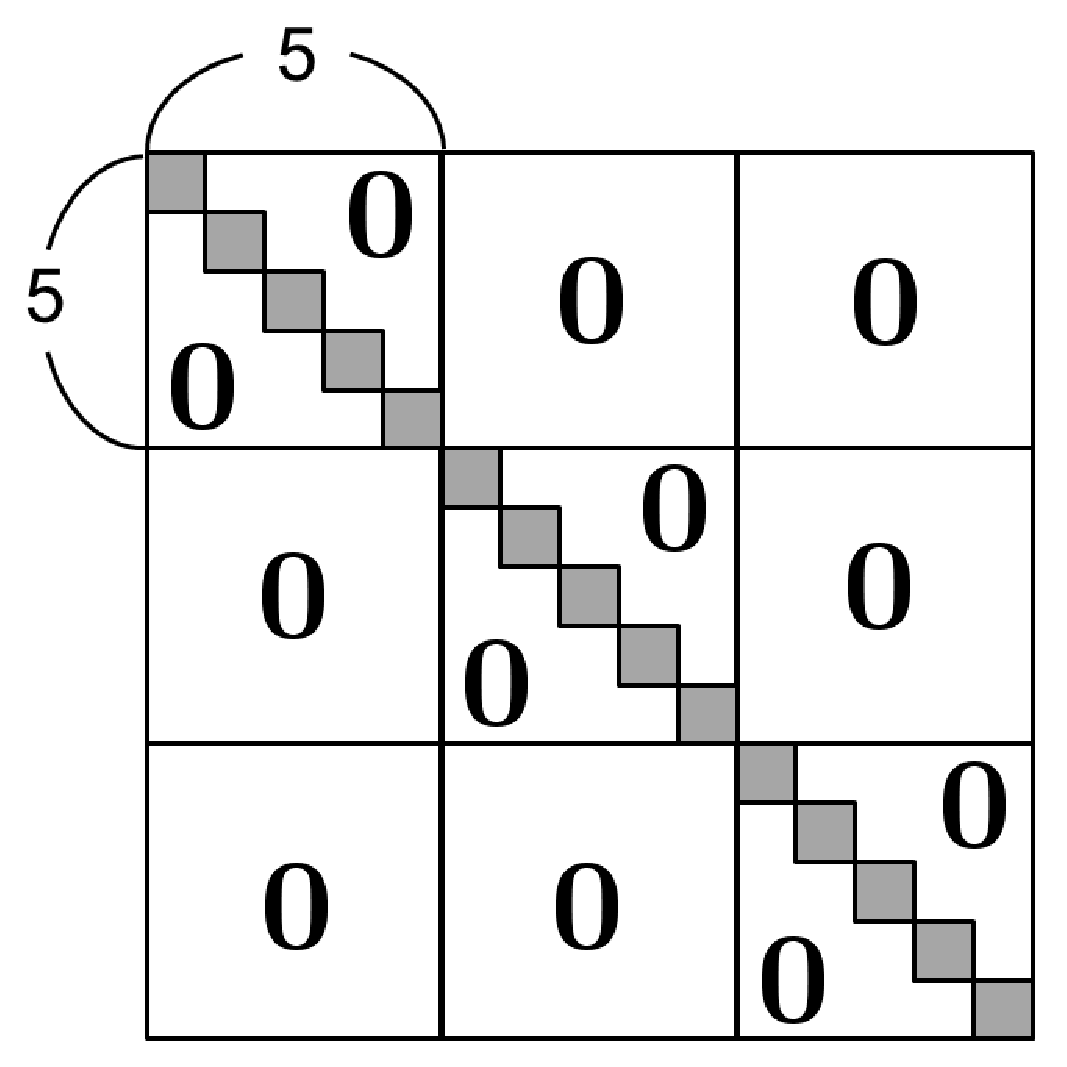
\includegraphics[width=0.8\hsize]{fig/GMM_1.eps}
      \\ (a) diagonal \\(without -c1 and -c2 option)
     \end{center}
    \vspace{3mm}
    \begin{center}
     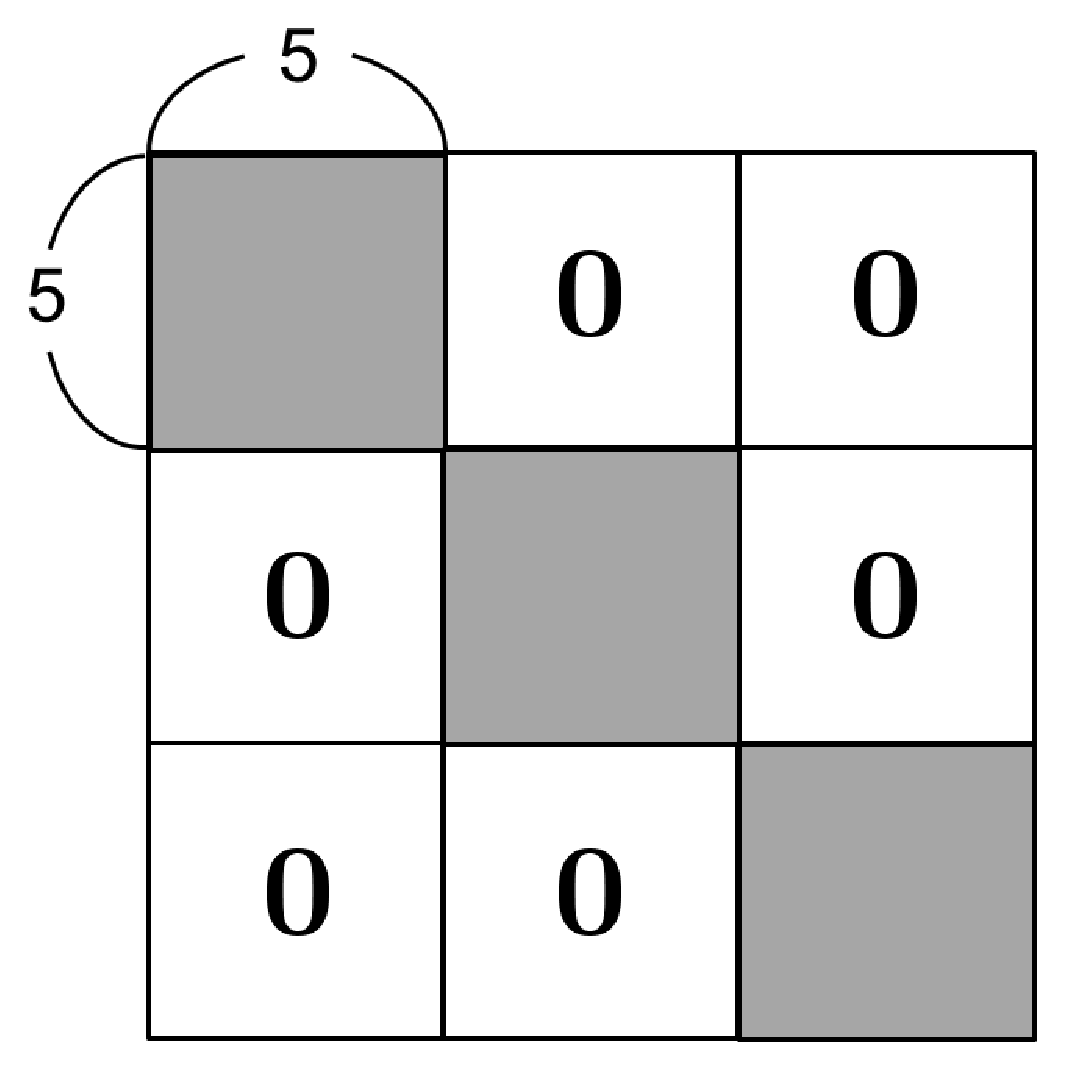
\includegraphics[width=0.8\hsize]{fig/GMM_3.eps}
    \\ (c) block-wise full covariance \\(with -c2 option)
    \end{center}
   \end{minipage}
   \begin{minipage}[b]{0.45\hsize}
    \begin{center}
     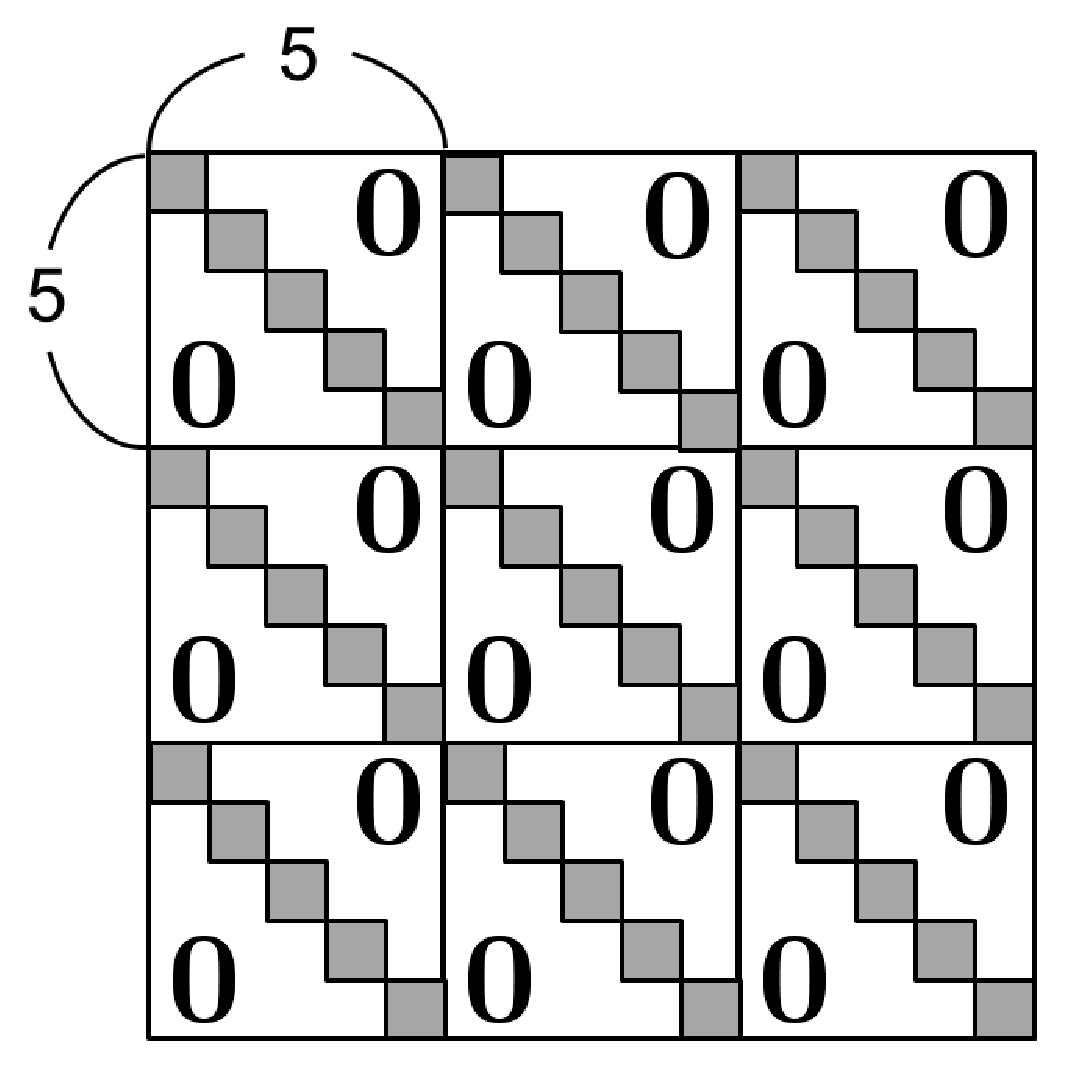
\includegraphics[width=0.8\hsize]{fig/GMM_2.eps}
     \\ (b) inter-block correlation \\(with -c1 option)
    \end{center}
    \vspace{3mm}
    \begin{center}
     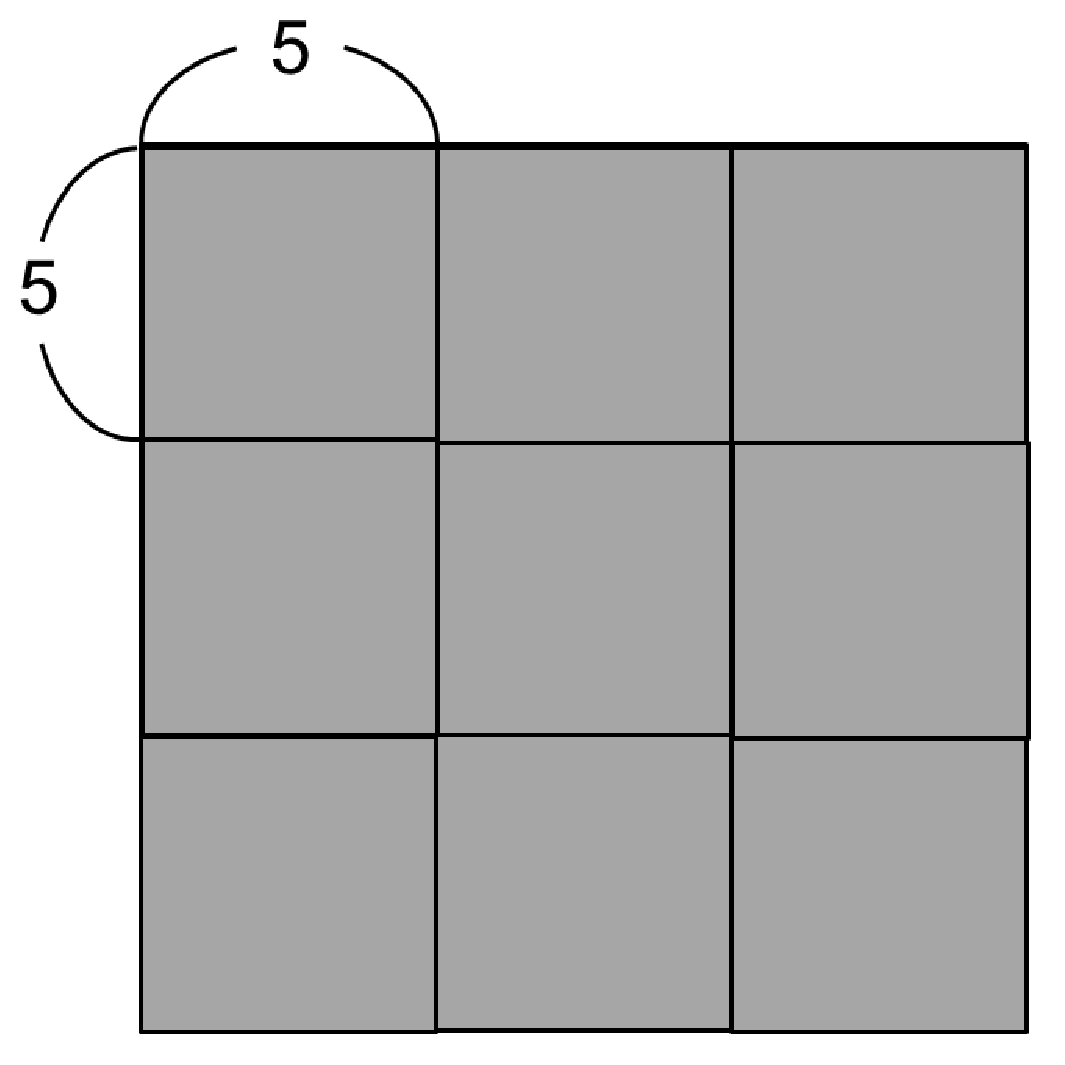
\includegraphics[width=0.8\hsize]{fig/GMM_4.eps}
     \\ (d) full covariance \\(with both -c1 and -c2 option)
    \end{center}
   \end{minipage}
  \end{tabular}
 \end{center}
 \caption{Examples of the structure of covariance matrix}
 \label{fig:gmm_c1}
 \end{figure}
\end{qsection}

\newpage

\begin{qsection}{NOTICE}
\begin{itemize}
\item The -e option specifies a threshold for the change of average
 log-likelihood for training data at each iteration.
\item The -F option specifies a GMM initial parameter file in which
weight, mean, and variance parameters must be aligned in the same
order as output.
\item The -B option specifies the size of each blocks in covariance matrix.
\item The -c1 and -c2 option must be used with -B option. Without -c1 and
-c2 option, a diagonal covariance can be obtained.
\end{itemize}
\end{qsection}

\begin{qsection}{SEE ALSO}
\hyperlink{gmmp}{gmmp},
\hyperlink{lbg}{lbg}
\end{qsection}

% ----------------------------------------------------------------- %
%             The Speech Signal Processing Toolkit (SPTK)           %
%             developed by SPTK Working Group                       %
%             http://sp-tk.sourceforge.net/                         %
% ----------------------------------------------------------------- %
%                                                                   %
%  Copyright (c) 1984-2007  Tokyo Institute of Technology           %
%                           Interdisciplinary Graduate School of    %
%                           Science and Engineering                 %
%                                                                   %
%                1996-2016  Nagoya Institute of Technology          %
%                           Department of Computer Science          %
%                                                                   %
% All rights reserved.                                              %
%                                                                   %
% Redistribution and use in source and binary forms, with or        %
% without modification, are permitted provided that the following   %
% conditions are met:                                               %
%                                                                   %
% - Redistributions of source code must retain the above copyright  %
%   notice, this list of conditions and the following disclaimer.   %
% - Redistributions in binary form must reproduce the above         %
%   copyright notice, this list of conditions and the following     %
%   disclaimer in the documentation and/or other materials provided %
%   with the distribution.                                          %
% - Neither the name of the SPTK working group nor the names of its %
%   contributors may be used to endorse or promote products derived %
%   from this software without specific prior written permission.   %
%                                                                   %
% THIS SOFTWARE IS PROVIDED BY THE COPYRIGHT HOLDERS AND            %
% CONTRIBUTORS "AS IS" AND ANY EXPRESS OR IMPLIED WARRANTIES,       %
% INCLUDING, BUT NOT LIMITED TO, THE IMPLIED WARRANTIES OF          %
% MERCHANTABILITY AND FITNESS FOR A PARTICULAR PURPOSE ARE          %
% DISCLAIMED. IN NO EVENT SHALL THE COPYRIGHT OWNER OR CONTRIBUTORS %
% BE LIABLE FOR ANY DIRECT, INDIRECT, INCIDENTAL, SPECIAL,          %
% EXEMPLARY, OR CONSEQUENTIAL DAMAGES (INCLUDING, BUT NOT LIMITED   %
% TO, PROCUREMENT OF SUBSTITUTE GOODS OR SERVICES; LOSS OF USE,     %
% DATA, OR PROFITS; OR BUSINESS INTERRUPTION) HOWEVER CAUSED AND ON %
% ANY THEORY OF LIABILITY, WHETHER IN CONTRACT, STRICT LIABILITY,   %
% OR TORT (INCLUDING NEGLIGENCE OR OTHERWISE) ARISING IN ANY WAY    %
% OUT OF THE USE OF THIS SOFTWARE, EVEN IF ADVISED OF THE           %
% POSSIBILITY OF SUCH DAMAGE.                                       %
% ----------------------------------------------------------------- %
\hypertarget{gmmp}{}
\name{gmmp}{calculation of GMM log-probability}{probability calculation}

\begin{synopsis}
\item [gmmp] [ --l $L$ ] [ --m $M$ ] [ --f ] [ --a ] [ --B $B1,B2,...$
] [ --c1 ] [ --c2 ] [ --D ] {\em gmmfile} [ {\em infile} ]
\end{synopsis}

\begin{qsection}{DESCRIPTION}
{\em gmmp} calculates GMM log-probabilities of input vectors from {\em
infile} (or standard input). 
The {\em gmmfile} has the same file format as the one generated by the {\em gmm} command,
i.e., {\em gmmfile} consists of $M$ mixture weights
$\bw$ and $M$ Gaussians with mean vector $\bmu$ and diagonal variance vector
$\bv$, each of length $L$:
\begin{align}
 \lambda =
 \left[\bw,\right.&\left.\bmu(0),\bv(0), \bmu(1), \bv(1),
 \ldots, \bmu(M-1), \bv(M-1)\right],\notag\\[2mm]
 \bw &=\left[ w(0), w(1), \ldots, w(M-1) \right],\notag\\
 \bmu(m) &=\left[\mu_m(0), \mu_m(1), \ldots, \mu_m(L-1)\right],\notag\\
 \bv(m) &=\left[\sigma_m^2(0), \sigma_m^2(1), \ldots,
 \sigma_m^2(L-1)\right].\notag
\end{align}


The input sequence consists of $T$ float vectors $\bx$, each of
size $L$:
\begin{displaymath}
 \bx(0), \bx(1), \dots, \bx(T-1).
\end{displaymath}
The result is a sequence of log-probabilities of input vectors:
\begin{displaymath}
 \log b(\bx(0)), \log b(\bx(1)), \ldots, \log b(\bx(T-1)),
\end{displaymath}
or an average log-probability (if -a option is used):
\begin{displaymath}
 \log P(\bX) = \frac{1}{T}\sum_{t=0}^{T-1}\log b(\bx(t)),
\end{displaymath}
where
\begin{align}
 &b(\bx(t)) =\sum_{m=0}^{M-1}
 w(m){\cal N}(\bx(t) \; ; \; \bmu(m),\bv(m)),\notag\\
 &{\cal N}(\bx(t) \; ; \; \bmu(m),\bv(m))%
  =\frac{1}{(2\pi)^{L/2}\prod_{l=0}^{L-1}\sigma_m(l)}%
  \exp{\left\{-\frac{1}{2}%
    \sum_{l=0}^{L-1}
    \frac{\left(x_t(l)-\mu_m(l)\right)^2}%
    {\sigma_m^2(l)}\right\}}.\notag
\end{align}

\end{qsection}

\begin{options}
 \argm{l}{L}{length of vector}{26}
 \argm{m}{M}{number of Gaussian components}{16}
 \argm{f}{}{full covariance}{FALSE}
 \argm{a}{}{print average log-probability}{FALSE}
 \desc[1ex]{(level 2)}
 \argm{B}{B1~B2~$\ldots$~Bn}{block size in covariance matrix,\\
                             where $(B1+B2+\ldots+Bn)=L$}{FALSE}
 \argm{c1}{}{inter-block correlation}{FALSE}
 \argm{c2}{}{full covariance in each block}{FALSE}
 \argm{D}{}{print log-probability of each block}{FALSE}
\end{options}

\begin{qsection}{EXAMPLE}
In the following example, frame log-probabilities of input data {\em
data.f} for GMM with 8 Gaussians {\em gmm.f} are written to {\em
probs.f}.

\begin{quote}
\verb! gmmp -m 8 gmm.f data.f > probs.f!
\end{quote}
\end{qsection}

\begin{qsection}{SEE ALSO}
\hyperlink{gmm}{gmm}
\end{qsection}

\name{gnorm}{$B0lHL2=%1%W%9%H%i%`$N%2%$%s$N@55,2=(B}{$B?.9f=hM}(B}

\begin{synopsis}
\item [gnorm] [ --m $M$ ] [ --g $G$ ] [ {\em infile} ]
\end{synopsis}

\begin{qsection}{DESCRIPTION}
$B@55,2=$5$l$F$$$J$$0lHL2=%1%W%9%H%i%`(B $c_\gamma(m)$ $B$r@55,2=$7!$(B
$BI8=`=PNO$K=PNO$7$^$9!%(B
\par
$B%G!<%?7A<0$OF~NO!$=PNO$H$b(Bfloat $B7A<0$G$9!%(B
\par
$B@55,2=$7$?0lHL2=%1%W%9%H%i%`(B $c_\gamma'(m)$ $B$O(B
\begin{displaymath}
c_\gamma'(m) = \frac{c_\gamma(m)}{1+\gamma c_\gamma(0)}, ~~~m>0
\end{displaymath}
$B$G5a$a$i$l$^$9!%$?$@$7!$%2%$%s9`(B $K = c_\gamma'(0)$ $B$O(B
\begin{displaymath}
K = \left\{
	\begin{array}{ll} \displaystyle
	  \left(\frac{1}{1+\gamma c_\gamma(0)}\right)^{1/\gamma},
		& 0<|\gamma|\leq 1 \\ \displaystyle
	  \exp c_\gamma(0),  & \gamma=0
	\end{array} \right.
\end{displaymath}
$B$H$J$j$^$9!%(B
\end{qsection}

\begin{options}
	\argm{m}{M}{$B0lHL2=%1%W%9%H%i%`$N<!?t!%(B}{25}
	\argm{g}{G}{$B0lHL2=%1%W%9%H%i%`$N$Y$-%Q%i%a!<%?(B $\gamma$ $B!%(B\\
			 $B$?$@$7!$(B$G>1.0$ $B$N$H$-$O(B $\gamma=-1/G$$B!%(B}{0}
\end{options}

\begin{qsection}{EXAMPLE}
float$B7A<0$N@55,2=$5$l$F$$$J$$0lHL2=%1%W%9%H%i%`%U%!%$%k(B 
{\em data.gcep} $(M=15, \gamma=-0.5)$ $B$r@55,2=$7!$(B
$B@55,2=0lHL2=%1%W%9%H%i%`$r(B {\em data.ngcep} $B$K=PNO$9$k(B:
\begin{quote}
 \verb!gnorm -m 15 -g 2 < data.gcep > data.ngcep!
\end{quote} 
\end{qsection}

\begin{qsection}{SEE ALSO}
 ignorm, gcep, mgcep, gc2gc, mgc2mgc, freqt
\end{qsection}

% ----------------------------------------------------------------
%       Speech Signal Processing Toolkit (SPTK): version 3.0
%                      SPTK Working Group
% 
%                Department of Computer Science
%                Nagoya Institute of Technology
%                             and
%   Interdisciplinary Graduate School of Science and Engineering
%                Tokyo Institute of Technology
%                   Copyright (c) 1984-2000
%                     All Rights Reserved.
% 
% Permission is hereby granted, free of charge, to use and
% distribute this software and its documentation without
% restriction, including without limitation the rights to use,
% copy, modify, merge, publish, distribute, sublicense, and/or
% sell copies of this work, and to permit persons to whom this
% work is furnished to do so, subject to the following conditions:
% 
%   1. The code must retain the above copyright notice, this list
%      of conditions and the following disclaimer.
% 
%   2. Any modifications must be clearly marked as such.
%                                                                        
% NAGOYA INSTITUTE OF TECHNOLOGY, TOKYO INSITITUTE OF TECHNOLOGY,
% SPTK WORKING GROUP, AND THE CONTRIBUTORS TO THIS WORK DISCLAIM
% ALL WARRANTIES WITH REGARD TO THIS SOFTWARE, INCLUDING ALL
% IMPLIED WARRANTIES OF MERCHANTABILITY AND FITNESS, IN NO EVENT
% SHALL NAGOYA INSTITUTE OF TECHNOLOGY, TOKYO INSITITUTE OF
% TECHNOLOGY, SPTK WORKING GROUP, NOR THE CONTRIBUTORS BE LIABLE
% FOR ANY SPECIAL, INDIRECT OR CONSEQUENTIAL DAMAGES OR ANY
% DAMAGES WHATSOEVER RESULTING FROM LOSS OF USE, DATA OR PROFITS,
% WHETHER IN AN ACTION OF CONTRACT, NEGLIGENCE OR OTHER TORTIOUS
% ACTION, ARISING OUT OF OR IN CONNECTION WITH THE USE OR
% PERFORMANCE OF THIS SOFTWARE.
% ----------------------------------------------------------------
%
\hypertarget{grlogsp}{}
\name{grlogsp}{draw a running log spectrum graph}{plotting graphs}

\begin{synopsis}
\item[grlogsp] [ --t ] [ --O $O$ ] [ --x $X$ ] [ --y $ymin$ ] [ --yy $YY$ ]
	       [ --yo $YO$ ] [ --p $P$ ] 
\item[\ ~~~~~~~~] [ --ln $LN$ ] [ --s $S$ ] [ --e $E$ ] [ --n $N$ ] [ --l $L$ ] 
\item[\ ~~~~~~~~] [ --c $comment1$ ] [ --c2 $comment2$ ] [ --c3 $comment3$ ]
		  [ {\em infile} ]
\end{synopsis}

\begin{qsection}{DESCRIPTION}
{\em grlogsp} converts a sequence of float-format log spectra 
from {\em infile} (or standard input) 
to a running spectrum plot in FP5301 plot format,
sending the result to standard output. 
The output can viewed with ``xgr''.

{\em grlogsp} is implemented as a shell script 
that uses the ``fig'' and ``fdrw'' commands.
\end{qsection}

\begin{options}
	\argm{t}{}{transpose x and y axes}{FALSE}
	\argm{O}{O}{origin of graph\\
		      \begin{minipage}{4cm}
		      \begin{tabular}{ccc}
			1 & ( 25,$YO$) & [mm] \\
			2 & ( 60,$YO$) & [mm] \\
			3 & ( 95,$YO$) & [mm] \\
			4 & (130,$YO$) & [mm] \\
			5 & (165,$YO$) & [mm]
		      \end{tabular}\\\hspace*{\fill}
		      \end{minipage}
		      \begin{minipage}{4cm}
			    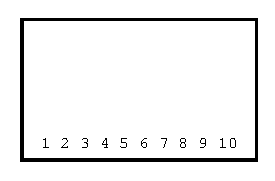
\includegraphics{fig/grlogsp-on.eps}
		      \end{minipage}\\\hspace*{\fill}\\
		    $(YO + 100 , X)$ [mm] if -t is specified.}{1}
	\argm{x}{X}{ $x$ scale\\
		       \begin{tabular}{cl}
			1 & normalized frequency($0 \sim 0.5$) \\
			2 & normalized frequency($0 \sim \pi$) \\
			4 & frequency($0 \sim 4$kHz) \\
			5 & frequency($0 \sim 5$kHz) \\
			8 & frequency($0 \sim 8$kHz) \\
			10 & frequency($0 \sim 10$kHz) \\
		       \end{tabular}\\\hspace*{\fill}}{1}
	\argm{y}{ymin}{ $y$ minimum}{-100}
	\argm{yy}{YY}{ $y$ scale [dB/10mm]}{100}
	\argm{yo}{YO}{ $y$ offset}{30}
	\argm{p}{p}{type of pen ($1 \sim 10$)}{2}
	\argm{ln}{LN}{style of line($0 \sim 5$).
                      please refer to fig command section.}{1}
	\argm{s}{S}{start frame number}{0}
	\argm{e}{E}{end frame number}{EOF}
	\argm{n}{N}{number of frame}{EOF}
	\argm{l}{L}{frame length.
                    Actually $\frac{L}{2}$ data are plotted.}{256}
	\argm{c, c2, c3}{\mbox{\em comment} 1 \sim 3}%
                        {comment for the graph}{N/A}
	\desc[1ex]{Usually, the options below do not need to be assigned.}
	\argm{W}{W}{width of the graph($\times 100$mm)}{0.25}
	\argm{H}{H}{height of the graph($\times 100$mm)}{1.5}
	\argm{z}{Z}{This option is used when data is written
                    recursively in the $y$ axis. the distance between
                    two graphs in the $y$ axis are given by $Z$.}{1}
	\argm{o}{xo \; yo}{origin of the graph.
                      if -o option exists, -O is not effective.}{95 30}
	\argm{g}{G}{type of frame of the graph($0 \sim 2$).
                    please refer to ``fig'' command section.}{2}
	\argm{cy}{cy}{first comment position}{-8}
	\argm{cy2}{cy2}{second comment position}{-14}
	\argm{cy3}{cy3}{third comment position}{-20}
	\argm{cs}{cs}{font size of the comments}{1}
	\argm{f}{f}{additional data file for fig}{NULL}
\end{options}

\begin{qsection}{EXAMPLE}
In this example, the magnitude of log spectrum is evaluated from
data in {\em data.f} file in float format, and the graph
with the running spectrum is sent in Postscript format to {\em data.ps}
file:
\begin{quote}
 \verb!frame < data.f | window |\! \\
 \verb!uels -m 15 | c2sp -m 15 |\! \\
 \verb!grlogsp | psgr > data.ps!
 \end{quote}
\end{qsection}

\begin{qsection}{SEE ALSO}
\hyperlink{fig}{fig},
\hyperlink{fdrw}{fdrw},
\hyperlink{xgr}{xgr},
\hyperlink{psgr}{psgr},
\hyperlink{glogsp}{glogsp},
\hyperlink{gwave}{gwave}
\end{qsection}

% ----------------------------------------------------------------
%       Speech Signal Processing Toolkit (SPTK): version 3.0
%                      SPTK Working Group
% 
%                Department of Computer Science
%                Nagoya Institute of Technology
%                             and
%   Interdisciplinary Graduate School of Science and Engineering
%                Tokyo Institute of Technology
%                   Copyright (c) 1984-2000
%                     All Rights Reserved.
% 
% Permission is hereby granted, free of charge, to use and
% distribute this software and its documentation without
% restriction, including without limitation the rights to use,
% copy, modify, merge, publish, distribute, sublicense, and/or
% sell copies of this work, and to permit persons to whom this
% work is furnished to do so, subject to the following conditions:
% 
%   1. The code must retain the above copyright notice, this list
%      of conditions and the following disclaimer.
% 
%   2. Any modifications must be clearly marked as such.
%                                                                        
% NAGOYA INSTITUTE OF TECHNOLOGY, TOKYO INSITITUTE OF TECHNOLOGY,
% SPTK WORKING GROUP, AND THE CONTRIBUTORS TO THIS WORK DISCLAIM
% ALL WARRANTIES WITH REGARD TO THIS SOFTWARE, INCLUDING ALL
% IMPLIED WARRANTIES OF MERCHANTABILITY AND FITNESS, IN NO EVENT
% SHALL NAGOYA INSTITUTE OF TECHNOLOGY, TOKYO INSITITUTE OF
% TECHNOLOGY, SPTK WORKING GROUP, NOR THE CONTRIBUTORS BE LIABLE
% FOR ANY SPECIAL, INDIRECT OR CONSEQUENTIAL DAMAGES OR ANY
% DAMAGES WHATSOEVER RESULTING FROM LOSS OF USE, DATA OR PROFITS,
% WHETHER IN AN ACTION OF CONTRACT, NEGLIGENCE OR OTHER TORTIOUS
% ACTION, ARISING OUT OF OR IN CONNECTION WITH THE USE OR
% PERFORMANCE OF THIS SOFTWARE.
% ----------------------------------------------------------------
%
\name{grpdelay}{$B74CY1d$r5a$a$k(B}{$B?.9f=hM}(B}
\begin{synopsis}
 \item[grpdelay] [ --l $L$ ] [ --m $M$ ] [ --a ] [ {\em infile} ] 
\end{synopsis}

\begin{qsection}{DESCRIPTION}
$B%U%!%$%k(B{\em infile}($B>JN,;~$OI8=`F~NO(B)$B$+$i%U%#%k%?78?t(B(FIR$B%U%#%k%?(B)
$B$rFI$_9~$_!$74CY1d$r=PNO$7$^$9!%%G!<%?7A<0$OF~=PNO$O6&$K(Bfloat$B7A<0$G$9!%(B

{\bf --m} $B%*%W%7%g%s$G(B $M$ $B$N;XDj$,$J$/!$$+$DF~NO7ONsD9$,(BFFT $B%5%$%:$h$jC;$$(B
$B>l9g!$F~NO7ONs$K(B0 $B$rIU2C$7$F(BFFT $B$r<B9T$7$^$9!%(B
{\bf --a}$B%*%W%7%g%s$,;XDj$5$l$?>l9g!$F~NO$NNm<!$N9`$O%2%$%s9`$H$7$F<h$j07$$(B
$B$^$9!%(B
\par
\[
\begin{array}{lll}
\mbox{$BF~NO7ONs(B} & 
\overbrace{\framebox[4.5cm]{$x_0, x_1, \ldots, x_{M}, 0,
					\ldots,0$}}^{L}  & \mbox{$B%U%#%k%?78?t(B}\\
		& \makebox[4.5cm]{0\hfill $L-1$} &
\end{array}
\]
\[
\begin{array}{lll}
\mbox{$B=PNO7ONs(B} & \overbrace{\framebox[4.5cm]{$\tau(\omega)$}}^{L/2+1} &
	   \mbox{$B74CY1d(B}\\
		& \makebox[4.5cm]{0\hfill $L-1$} &

\end{array}
\]
\end{qsection}

\begin{options}
	\argm{l}{L}{$B%U!<%j%(JQ49$N%5%$%:!%(B2$B$N$Y$->h$G;XDj!%(B}{256}
	\argm{m}{M}{$B%U%#%k%?$N<!?t!%(B}{L-1}
	\argm{a}{}{$BF~NO7ONs$r(BAR$B%U%#%k%?$N78?t$H$_$J$9!%(B}{FALSE}
\end{options}


\begin{qsection}{EXAMPLE}
$BEAC#4X?t(B
\begin{displaymath}
  H(z)=\frac{1}{1+0.9z^{-1}}
\end{displaymath}
$B$r$b$D%U%#%k%?$N%$%s%Q%k%91~Ez$N72CY1d$r5a$a!$2hLL$K%W%m%C%H$5$;$k(B:
\begin{quote}
\verb! impluse | dfs -a 1 0.9 | grpdelay | fdrw | xgr !
\end{quote}  
\end{qsection}

\begin{qsection}{SEE ALSO}
delay, phase
\end{qsection}

%\begin{qsection}{BUGS}
% FFT$B$N%5%$%:$O(B1024$B0J2<$G$9!%(B
%\end{qsection}

% ----------------------------------------------------------------- %
%             The Speech Signal Processing Toolkit (SPTK)           %
%             developed by SPTK Working Group                       %
%             http://sp-tk.sourceforge.net/                         %
% ----------------------------------------------------------------- %
%                                                                   %
%  Copyright (c) 1984-2007  Tokyo Institute of Technology           %
%                           Interdisciplinary Graduate School of    %
%                           Science and Engineering                 %
%                                                                   %
%                1996-2013  Nagoya Institute of Technology          %
%                           Department of Computer Science          %
%                                                                   %
% All rights reserved.                                              %
%                                                                   %
% Redistribution and use in source and binary forms, with or        %
% without modification, are permitted provided that the following   %
% conditions are met:                                               %
%                                                                   %
% - Redistributions of source code must retain the above copyright  %
%   notice, this list of conditions and the following disclaimer.   %
% - Redistributions in binary form must reproduce the above         %
%   copyright notice, this list of conditions and the following     %
%   disclaimer in the documentation and/or other materials provided %
%   with the distribution.                                          %
% - Neither the name of the SPTK working group nor the names of its %
%   contributors may be used to endorse or promote products derived %
%   from this software without specific prior written permission.   %
%                                                                   %
% THIS SOFTWARE IS PROVIDED BY THE COPYRIGHT HOLDERS AND            %
% CONTRIBUTORS "AS IS" AND ANY EXPRESS OR IMPLIED WARRANTIES,       %
% INCLUDING, BUT NOT LIMITED TO, THE IMPLIED WARRANTIES OF          %
% MERCHANTABILITY AND FITNESS FOR A PARTICULAR PURPOSE ARE          %
% DISCLAIMED. IN NO EVENT SHALL THE COPYRIGHT OWNER OR CONTRIBUTORS %
% BE LIABLE FOR ANY DIRECT, INDIRECT, INCIDENTAL, SPECIAL,          %
% EXEMPLARY, OR CONSEQUENTIAL DAMAGES (INCLUDING, BUT NOT LIMITED   %
% TO, PROCUREMENT OF SUBSTITUTE GOODS OR SERVICES; LOSS OF USE,     %
% DATA, OR PROFITS; OR BUSINESS INTERRUPTION) HOWEVER CAUSED AND ON %
% ANY THEORY OF LIABILITY, WHETHER IN CONTRACT, STRICT LIABILITY,   %
% OR TORT (INCLUDING NEGLIGENCE OR OTHERWISE) ARISING IN ANY WAY    %
% OUT OF THE USE OF THIS SOFTWARE, EVEN IF ADVISED OF THE           %
% POSSIBILITY OF SUCH DAMAGE.                                       %
% ----------------------------------------------------------------- %
\hypertarget{gseries}{}
\name{gseries}{draw a discrete series}{plotting graphs}

\begin{synopsis}
\item[gseries] [ --F $F$] [ --s $S$ ] [ --e $E$ ] [ --n $N$ ] [ --i $I$ ] [ --y $ymax$ ]
               [ --y2 $ymin$ ] [--m $M$ ] 
\item[\ ~~~~~~~~] [ --p $P$ ] [ --magic $magic$ ] [ --MAGIC $MAGIC$ ] [ +{\em type} ]  [ {\em infile} ]

\end{synopsis}

\begin{qsection}{DESCRIPTION}
{\em gseries} converts discrete series data
from {\em infile} (or standard input) to FP5301 plot format, 
sending the result to standard output. 
The output can viewed with \hyperlink{xgr}{xgr}.

{\em gseries} is implemented as a shell script 
that uses the \hyperlink{fig}{fig} command.
\end{qsection}

\begin{options}
        \argm{F}{F}{factor}{1}
        \argm{s}{S}{start point}{0}
        \argm{e}{E}{end point}{EOF}
        \argm{n}{N}{data number of one screen\\
                    if this option is omitted,
                    all of the data is plotted on one screen.}{N/A}
        \argm{i}{I}{number of screen}{5}
        \argm{y}{ymax}{maximum amplitude\\
                       if this option is omitted,
                       ymax is maximum value of the input data.}{N/A}
        \argm{y2}{ymin}{minimum amplitude}{-YMAX}
        \argm{m}{M}{mark type}{1}
        \argm{p}{P}{pen type($1 \sim 10$)}{1}
        \argm{magic}{magic}{remove magic number}{FALSE}
        \argm{MAGIC}{MAGIC}{replace magic number by $MAGIC$ \\
                            if -magic option is not given, return error.\\
                        if -magic or -MAGIC option is given multiple
                        times, also return error.}{FALSE}
        \argp{t}{Input data format\\ 
                \begin{tabular}{llcll} \\[-1ex]
                        c & char (1 byte) & \quad &
                        C & unsigned char (1 byte) \\
                        s & short (2 bytes) & \quad &
                        S & unsigned short (2 bytes) \\
                        i3 & int (3 bytes) & \quad &
                        I3 & unsigned int (3 bytes) \\
                        i & int (4 bytes) & \quad &
                        I & unsigned int (4 bytes) \\
                        l & long (4 bytes) & \quad &
                        L & unsigned long (4 bytes) \\
                        le & long long (8 bytes) & \quad &
                        LE & unsigned long long (8 bytes) \\
                        f & float (4 bytes) & \quad &
                        d & double (8 bytes) \\
                        de & long double (12 bytes) & \quad &
                \end{tabular}}{f}
\end{options}

\begin{qsection}{EXAMPLE}
 In the following example, {\em gseries} reads impulse response
 in float format from {\em data.f} and writes the output
 in encapsulated Postscript format to {\em data.eps}.
 \begin{quote}
 \verb!gseries +f < data.f | psgr > data.eps!
 \end{quote}
The following example replaces the magic number 0 in {\em data.f} by 1.0 and
writes the output to {\em data.eps}.
\begin{quote}
  \verb!gseriese +f -magic 0 -MAGIC 1.0 < data.f | \!\\
  \verb!psgr > data.eps!
\end{quote}
Also, the following example removes the magic number 0 in {\em data.f}.
\begin{quote}
  \verb!gseriese +f -magic 0 < data.f | psgr > data.eps!
\end{quote}
\end{qsection}

\begin{qsection}{SEE ALSO}
\hyperlink{fig}{fig},
\hyperlink{fdrw}{fdrw},
\hyperlink{xgr}{xgr},
\hyperlink{psgr}{psgr},
\hyperlink{glogsp}{glogsp},
\hyperlink{grlogsp}{grlogsp},
\hyperlink{gwave}{gwave}
\end{qsection}

% ----------------------------------------------------------------- %
%             The Speech Signal Processing Toolkit (SPTK)           %
%             developed by SPTK Working Group                       %
%             http://sp-tk.sourceforge.net/                         %
% ----------------------------------------------------------------- %
%                                                                   %
%  Copyright (c) 1984-2007  Tokyo Institute of Technology           %
%                           Interdisciplinary Graduate School of    %
%                           Science and Engineering                 %
%                                                                   %
%                1996-2016  Nagoya Institute of Technology          %
%                           Department of Computer Science          %
%                                                                   %
% All rights reserved.                                              %
%                                                                   %
% Redistribution and use in source and binary forms, with or        %
% without modification, are permitted provided that the following   %
% conditions are met:                                               %
%                                                                   %
% - Redistributions of source code must retain the above copyright  %
%   notice, this list of conditions and the following disclaimer.   %
% - Redistributions in binary form must reproduce the above         %
%   copyright notice, this list of conditions and the following     %
%   disclaimer in the documentation and/or other materials provided %
%   with the distribution.                                          %
% - Neither the name of the SPTK working group nor the names of its %
%   contributors may be used to endorse or promote products derived %
%   from this software without specific prior written permission.   %
%                                                                   %
% THIS SOFTWARE IS PROVIDED BY THE COPYRIGHT HOLDERS AND            %
% CONTRIBUTORS "AS IS" AND ANY EXPRESS OR IMPLIED WARRANTIES,       %
% INCLUDING, BUT NOT LIMITED TO, THE IMPLIED WARRANTIES OF          %
% MERCHANTABILITY AND FITNESS FOR A PARTICULAR PURPOSE ARE          %
% DISCLAIMED. IN NO EVENT SHALL THE COPYRIGHT OWNER OR CONTRIBUTORS %
% BE LIABLE FOR ANY DIRECT, INDIRECT, INCIDENTAL, SPECIAL,          %
% EXEMPLARY, OR CONSEQUENTIAL DAMAGES (INCLUDING, BUT NOT LIMITED   %
% TO, PROCUREMENT OF SUBSTITUTE GOODS OR SERVICES; LOSS OF USE,     %
% DATA, OR PROFITS; OR BUSINESS INTERRUPTION) HOWEVER CAUSED AND ON %
% ANY THEORY OF LIABILITY, WHETHER IN CONTRACT, STRICT LIABILITY,   %
% OR TORT (INCLUDING NEGLIGENCE OR OTHERWISE) ARISING IN ANY WAY    %
% OUT OF THE USE OF THIS SOFTWARE, EVEN IF ADVISED OF THE           %
% POSSIBILITY OF SUCH DAMAGE.                                       %
% ----------------------------------------------------------------- %
\hypertarget{gwave}{}
\name{gwave}{draw a waveform}{plotting graphs}

\begin{synopsis}
\item[gwave] [ --F $F$] [ --s $S$ ] [ --e $E$ ] [ --n $N$ ] [ --i $I$ ] [ --y $ymax$ ]
               [ --y2 $ymin$ ] [ --p $P$ ] 
\item[\ ~~~~~~~~] [ +{\em type} ]  [ {\em infile} ]

\end{synopsis}

\begin{qsection}{DESCRIPTION}
{\em gwave} converts speech waveform data 
from {\em infile} (or standard input) to FP5301 plot format, 
sending the result to standard output. 
The output can viewed with \hyperlink{xgr}{xgr}.

{\em gwave} is implemented as a shell script 
that uses the \hyperlink{fig}{fig} and \hyperlink{fdrw}{fdrw} commands.
\end{qsection}

\begin{options}
        \argm{F}{F}{factor}{1}
        \argm{s}{S}{start point}{0}
        \argm{e}{E}{end point}{EOF}
        \argm{n}{N}{data number of one screen\\
                    if this option is omitted,
                    all of the data is plotted on one screen.}{N/A}
        \argm{i}{I}{number of screen}{5}
        \argm{y}{ymax}{maximum amplitude\\
                       if this option is omitted,
                       ymax is maximum value of the input data.}{N/A}
        \argm{y2}{ymin}{minimum amplitude}{-YMAX}
        \argm{p}{P}{pen type($1 \sim 10$)}{1}
        \argp{t}{Input data format\\ 
                \begin{tabular}{llcll} \\[-1ex]
                        c & char (1 byte) & \quad &
                        C & unsigned char (1 byte) \\
                        s & short (2 bytes) & \quad &
                        S & unsigned short (2 bytes) \\
                        i3 & int (3 bytes) & \quad &
                        I3 & unsigned int (3 bytes) \\
                        i & int (4 bytes) & \quad &
                        I & unsigned int (4 bytes) \\
                        l & long (4 bytes) & \quad &
                        L & unsigned long (4 bytes) \\
                        le & long long (8 bytes) & \quad &
                        LE & unsigned long long (8 bytes) \\
                        f & float (4 bytes) & \quad &
                        d & double (8 bytes) \\
                        de & long double (12 bytes) & \quad &
                \end{tabular}}{f}
\end{options}

\begin{qsection}{EXAMPLE}
This example reads speech waveform file in float format from
{\em data.f} and writes the output in Postscript format to
{\em data.ps}.
\begin{quote}
 \verb!gwave +f < data.f | psgr > data.ps!
 \end{quote}
\end{qsection}

\begin{qsection}{NOTICE}
\begin{itemize}
\item If options of amplitude are not used, value of amplitude is
automatically determined.
\item If --n option is not used, entire waveform is displayed.
\end{itemize}
\end{qsection}

\begin{qsection}{SEE ALSO}
\hyperlink{fig}{fig},
\hyperlink{fdrw}{fdrw},
\hyperlink{xgr}{xgr},
\hyperlink{psgr}{psgr},
\hyperlink{glogsp}{glogsp},
\hyperlink{grlogsp}{grlogsp}
\end{qsection}

\name{histogram}{histogram}{evaluation of the data}

\begin{synopsis}
\item [histogram] [ --l $L$ ] [ --i $I$ ] [ --j $J$ ] [ --s $S$ ] [ --n ] 
                  [ {\em infile} ] 
\end{synopsis}

\begin{qsection}{DESCRIPTION}
This command evaluates the histogram from the assigned file
and sends the results to the standard output.
\par
Input and output data are in float format.
If a graph is wanted, please send the output of ``histogram'' to ``fdrw''.
\par
In case a data value is outside of the assigned interval,
the histogram will evaluate its output but the return value of
the command will be different from $0$.
\end{qsection}

\begin{options}
        \argm{l}{L}{frame size\\
          \begin{tabular}{ll}\\ [-1zh]
            $L>0$ & evaluate the histogram for every frame\\
            $L=0$ & evaluate the histogram for the whole file\\
          \end{tabular}\\\hspace*{\fill}}{0}
        \argm{i}{I}{infimum}{0.0}
        \argm{j}{J}{supremum}{1.0}
        \argm{s}{S}{step size}{0.1}
        \argm{n}{}{normalization}{FALSE}
\end{options}

\begin{qsection}{EXAMPLE}
The example below plots the histogram of the speech waveform file
{\em data.f} in float format.
\begin{quote}
 \verb!histogram -i -16000 -j 16000 -s 100 data.f | fdrw | xgr!
\end{quote} 
\end{qsection}

\begin{qsection}{SEE ALSO}
 average
\end{qsection}

% ----------------------------------------------------------------- %
%             The Speech Signal Processing Toolkit (SPTK)           %
%             developed by SPTK Working Group                       %
%             http://sp-tk.sourceforge.net/                         %
% ----------------------------------------------------------------- %
%                                                                   %
%  Copyright (c) 1984-2007  Tokyo Institute of Technology           %
%                           Interdisciplinary Graduate School of    %
%                           Science and Engineering                 %
%                                                                   %
%                1996-2016  Nagoya Institute of Technology          %
%                           Department of Computer Science          %
%                                                                   %
% All rights reserved.                                              %
%                                                                   %
% Redistribution and use in source and binary forms, with or        %
% without modification, are permitted provided that the following   %
% conditions are met:                                               %
%                                                                   %
% - Redistributions of source code must retain the above copyright  %
%   notice, this list of conditions and the following disclaimer.   %
% - Redistributions in binary form must reproduce the above         %
%   copyright notice, this list of conditions and the following     %
%   disclaimer in the documentation and/or other materials provided %
%   with the distribution.                                          %
% - Neither the name of the SPTK working group nor the names of its %
%   contributors may be used to endorse or promote products derived %
%   from this software without specific prior written permission.   %
%                                                                   %
% THIS SOFTWARE IS PROVIDED BY THE COPYRIGHT HOLDERS AND            %
% CONTRIBUTORS "AS IS" AND ANY EXPRESS OR IMPLIED WARRANTIES,       %
% INCLUDING, BUT NOT LIMITED TO, THE IMPLIED WARRANTIES OF          %
% MERCHANTABILITY AND FITNESS FOR A PARTICULAR PURPOSE ARE          %
% DISCLAIMED. IN NO EVENT SHALL THE COPYRIGHT OWNER OR CONTRIBUTORS %
% BE LIABLE FOR ANY DIRECT, INDIRECT, INCIDENTAL, SPECIAL,          %
% EXEMPLARY, OR CONSEQUENTIAL DAMAGES (INCLUDING, BUT NOT LIMITED   %
% TO, PROCUREMENT OF SUBSTITUTE GOODS OR SERVICES; LOSS OF USE,     %
% DATA, OR PROFITS; OR BUSINESS INTERRUPTION) HOWEVER CAUSED AND ON %
% ANY THEORY OF LIABILITY, WHETHER IN CONTRACT, STRICT LIABILITY,   %
% OR TORT (INCLUDING NEGLIGENCE OR OTHERWISE) ARISING IN ANY WAY    %
% OUT OF THE USE OF THIS SOFTWARE, EVEN IF ADVISED OF THE           %
% POSSIBILITY OF SUCH DAMAGE.                                       %
% ----------------------------------------------------------------- %
\hypertarget{idct}{}
\name{idct}{Inverse DCT-II}{signal processing}

\begin{synopsis}
 \item[idct] [ --l $L$ ] [ --c ] [ --d ] [ {\em infile} ]
\end{synopsis}

\begin{qsection}{DESCRIPTION}
{\em idct} calculates the Inverse Discrete Cosine Transform II (IDCT-II)
of input data in {\em infile} (or standard input),
sending the results to standard output.
The input and output data is in float format, arranged as follows.
\begin{center}
 \leavevmode
 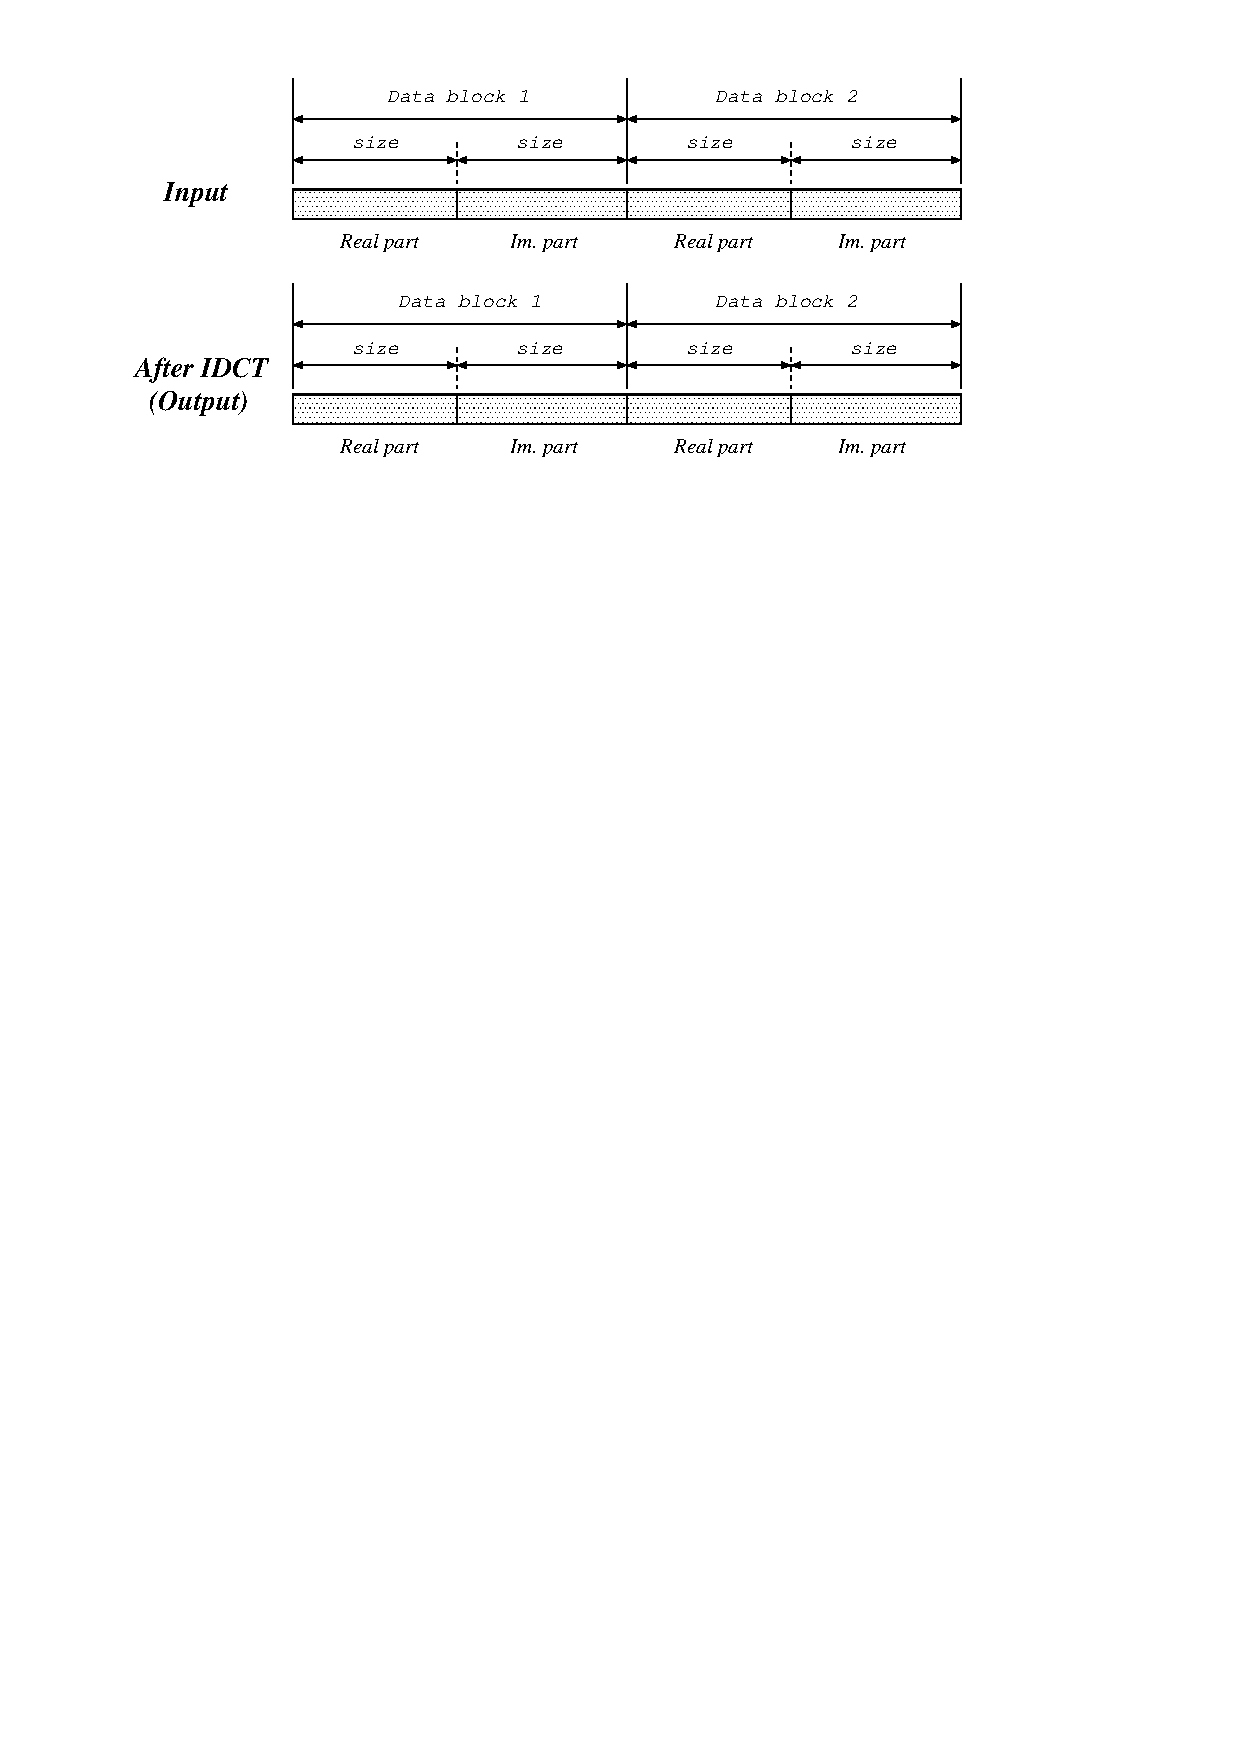
\includegraphics{fig/idct.pdf}
\end{center}
The Inverse Discrete Cosine Transformation II is given by
\begin{displaymath}
 x_{l} = \sqrt{\frac{2}{L}}c_{l}\sum_{k=0}^{L-1}
 X_{k}
 \cos\left\{\frac{\pi}{L} \left( k + \frac{1}{2} \right) l\right\},
\;\;\; l = 0, 1, \cdots, L
\end{displaymath}
where
 \begin{displaymath}
c_{l}= \begin{cases}
         \;\;1 & ( 1 \le l \le L - 1 ) \\
         \;\; 1 / \sqrt{2} & (l = 0)
        \end{cases}
 \end{displaymath}
\par
\end{qsection}

\begin{options}
        \argm{l}{L}{IDCT size}{256}
        \argm{c}{}{use complex number}{FALSE}
        \argm{d}{}{don't use FFT algorithm}{FALSE}
\end{options}

\begin{qsection}{EXAMPLE}
In this example, the IDCT is evaluated from a complex-valued data file
{\em data.f} in float format
(real part: 256 points, imaginary part: 256 points),
and the output is written to {\em data.idct}:
\begin{quote}
  \verb!idct data.f -l 256 -c > data.idct!
\end{quote}
\end{qsection}

\begin{qsection}{SEE ALSO}
 \hyperlink{fft}{fft},
 \hyperlink{dct}{dct}
\end{qsection}

% ----------------------------------------------------------------
%       Speech Signal Processing Toolkit (SPTK): version 3.0
%                      SPTK Working Group
% 
%                Department of Computer Science
%                Nagoya Institute of Technology
%                             and
%   Interdisciplinary Graduate School of Science and Engineering
%                Tokyo Institute of Technology
%                   Copyright (c) 1984-2000
%                     All Rights Reserved.
% 
% Permission is hereby granted, free of charge, to use and
% distribute this software and its documentation without
% restriction, including without limitation the rights to use,
% copy, modify, merge, publish, distribute, sublicense, and/or
% sell copies of this work, and to permit persons to whom this
% work is furnished to do so, subject to the following conditions:
% 
%   1. The code must retain the above copyright notice, this list
%      of conditions and the following disclaimer.
% 
%   2. Any modifications must be clearly marked as such.
%                                                                        
% NAGOYA INSTITUTE OF TECHNOLOGY, TOKYO INSITITUTE OF TECHNOLOGY,
% SPTK WORKING GROUP, AND THE CONTRIBUTORS TO THIS WORK DISCLAIM
% ALL WARRANTIES WITH REGARD TO THIS SOFTWARE, INCLUDING ALL
% IMPLIED WARRANTIES OF MERCHANTABILITY AND FITNESS, IN NO EVENT
% SHALL NAGOYA INSTITUTE OF TECHNOLOGY, TOKYO INSITITUTE OF
% TECHNOLOGY, SPTK WORKING GROUP, NOR THE CONTRIBUTORS BE LIABLE
% FOR ANY SPECIAL, INDIRECT OR CONSEQUENTIAL DAMAGES OR ANY
% DAMAGES WHATSOEVER RESULTING FROM LOSS OF USE, DATA OR PROFITS,
% WHETHER IN AN ACTION OF CONTRACT, NEGLIGENCE OR OTHER TORTIOUS
% ACTION, ARISING OUT OF OR IN CONNECTION WITH THE USE OR
% PERFORMANCE OF THIS SOFTWARE.
% ----------------------------------------------------------------
%
\name{ifft}{$BJ#AG?tNs$N9bB.5U%U!<%j%(JQ49(B}{$B?.9f=hM}(B}

\begin{synopsis}
\item[ifft] [ --l $L$ ]  [ --\{ R $|$ I \} ] [ {\em infile} ] 
\end{synopsis}

\begin{qsection}{DESCRIPTION}
{\em ifft} $B$O!$J#AG?t$GM?$($i$l$k%G!<%?Ns$r(B{\em infile}$B$+$iFI$_9~$s$G(B
$B5U%U!<%j%(JQ49$r9T$J$$!$7k2L$rI8=`=PNO$K=PNO$7$^$9!%(B
$BF~NO$O(Bfloat $B7A<0$G!$<BIt$r(B $L$ $B8DJB$Y$?8e$K5uIt$r(B $L$ $B8DJB$Y$?7A$K(B
$B$J$j$^$9!%(B
\begin{center}
 \leavevmode
 \epsffile{fig/ifft.eps} 
\end{center}
\end{qsection}

\begin{options}
	\argm{l}{L}{$B5U%U!<%j%(JQ49$N%5%$%:!%(B2$B$N$Y$->h$G;XDj!%(B}{256}
	\argm{R}{}{$B5UJQ49$N7k2L$N<BIt$N$_$r=PNO!%(B}{FALSE}
	\argm{I}{}{$B5UJQ49$N7k2L$N5uIt$N$_$r=PNO!%(B}{FALSE}
\end{options}

\begin{qsection}{EXAMPLE}
float$B7A<0$N%U%!%$%k(B {\em data.f} $B$K$"$k%G!<%?Ns!J<BIt(B256$BE@!$5uIt(B256$BE@!K$N(B $B5U(BDFT $B$r5a$a!$(Bdata.ifft$B$K=PNO$9$k(B:
\begin{quote}
  \verb!ifft data.f -l 256 > data.ifft!
\end{quote}
\end{qsection}

\begin{qsection}{SEE ALSO}
 fft, fft2, fftr, fftr2, ifft2
\end{qsection}

%  ---------------------------------------------------------------  %
%            Speech Signal Processing Toolkit (SPTK)                %
%                      SPTK Working Group                           %
%                                                                   %
%                  Department of Computer Science                   %
%                  Nagoya Institute of Technology                   %
%                               and                                 %
%   Interdisciplinary Graduate School of Science and Engineering    %
%                  Tokyo Institute of Technology                    %
%                                                                   %
%                     Copyright (c) 1984-2007                       %
%                       All Rights Reserved.                        %
%                                                                   %
%  Permission is hereby granted, free of charge, to use and         %
%  distribute this software and its documentation without           %
%  restriction, including without limitation the rights to use,     %
%  copy, modify, merge, publish, distribute, sublicense, and/or     %
%  sell copies of this work, and to permit persons to whom this     %
%  work is furnished to do so, subject to the following conditions: %
%                                                                   %
%    1. The source code must retain the above copyright notice,     %
%       this list of conditions and the following disclaimer.       %
%                                                                   %
%    2. Any modifications to the source code must be clearly        %
%       marked as such.                                             %
%                                                                   %
%    3. Redistributions in binary form must reproduce the above     %
%       copyright notice, this list of conditions and the           %
%       following disclaimer in the documentation and/or other      %
%       materials provided with the distribution.  Otherwise, one   %
%       must contact the SPTK working group.                        %
%                                                                   %
%  NAGOYA INSTITUTE OF TECHNOLOGY, TOKYO INSTITUTE OF TECHNOLOGY,   %
%  SPTK WORKING GROUP, AND THE CONTRIBUTORS TO THIS WORK DISCLAIM   %
%  ALL WARRANTIES WITH REGARD TO THIS SOFTWARE, INCLUDING ALL       %
%  IMPLIED WARRANTIES OF MERCHANTABILITY AND FITNESS, IN NO EVENT   %
%  SHALL NAGOYA INSTITUTE OF TECHNOLOGY, TOKYO INSTITUTE OF         %
%  TECHNOLOGY, SPTK WORKING GROUP, NOR THE CONTRIBUTORS BE LIABLE   %
%  FOR ANY SPECIAL, INDIRECT OR CONSEQUENTIAL DAMAGES OR ANY        %
%  DAMAGES WHATSOEVER RESULTING FROM LOSS OF USE, DATA OR PROFITS,  %
%  WHETHER IN AN ACTION OF CONTRACT, NEGLIGENCE OR OTHER TORTUOUS   %
%  ACTION, ARISING OUT OF OR IN CONNECTION WITH THE USE OR          %
%  PERFORMANCE OF THIS SOFTWARE.                                    %
%                                                                   %
%  ---------------------------------------------------------------  %
%
\hypertarget{ifft2}{}
\name{ifft2}{2-dimensional inverse FFT for complex sequence}{signal processing}

\begin{synopsis}
\item[ifft2] [ --l $L$ ] [ +r ] [ --t ] [ --c ] [ --q ] 
	     [ --\{ R $|$ I \} ] [ {\em infile} ]
\end{synopsis}

\begin{qsection}{DESCRIPTION}
{\em ifft} calculates the 2-dimensional Inverse Discrete Fourier Transform
(IDFT) of complex-valued data from {\em infile} (or standard input), 
sending the results to standard output.
The input and output data is in float format, arranged as follows.
\begin{center}
\leavevmode
\includegraphics{fig/ifft2.eps}
\end{center}
\end{qsection}

\begin{options}
	\argm{l}{L}{FFT size power of 2}{64}
	\argp{{\bf r}}{regard input as real values rather than complex values}{FALSE}
	\argm{t}{}{Output results in transposed form (see also \hyperlink{fft2}{fft2}).}{FALSE}
	\argm{c}{}{When results are transposed, 1 boundary data is copied from the
	opposite side, and then output $(L+1)\times (L+1)$ data (see also \hyperlink{fft2}{fft2}).}{FALSE}
	\argm{q}{}{Output first $1/4$ data of FFT results only.
		   As in the above c option, boundary data is compensated and 
		   $(\frac{L}{2}+1)\times(\frac{L}{2}+1)$ data are output.
		\begin{center}
		\leavevmode
		\includegraphics{fig/fft2-quad.eps}
		\end{center}~}{FALSE} %\hspace*{\fill}
	\argm{R}{}{output only real part}{FALSE}
	\argm{I}{}{output only imaginary part}{FALSE}
\end{options}

\begin{qsection}{EXAMPLE}
This example reads a sequence of 2-dimensional complex numbers in float format
from {\em data.f} file, evaluates its 2-dimensional IDFT and outputs it to {\em
data.dft} file:
\begin{quote}
  \verb!ifft2 -A < data.f > data.ifft2!
\end{quote}
\end{qsection}

\begin{qsection}{SEE ALSO}
\hyperlink{fft}{fft},
\hyperlink{fft2}{fft2},
\hyperlink{ifft}{ifft}
\end{qsection}

% ----------------------------------------------------------------- %
%             The Speech Signal Processing Toolkit (SPTK)           %
%             developed by SPTK Working Group                       %
%             http://sp-tk.sourceforge.net/                         %
% ----------------------------------------------------------------- %
%                                                                   %
%  Copyright (c) 1984-2007  Tokyo Institute of Technology           %
%                           Interdisciplinary Graduate School of    %
%                           Science and Engineering                 %
%                                                                   %
%                1996-2016  Nagoya Institute of Technology          %
%                           Department of Computer Science          %
%                                                                   %
% All rights reserved.                                              %
%                                                                   %
% Redistribution and use in source and binary forms, with or        %
% without modification, are permitted provided that the following   %
% conditions are met:                                               %
%                                                                   %
% - Redistributions of source code must retain the above copyright  %
%   notice, this list of conditions and the following disclaimer.   %
% - Redistributions in binary form must reproduce the above         %
%   copyright notice, this list of conditions and the following     %
%   disclaimer in the documentation and/or other materials provided %
%   with the distribution.                                          %
% - Neither the name of the SPTK working group nor the names of its %
%   contributors may be used to endorse or promote products derived %
%   from this software without specific prior written permission.   %
%                                                                   %
% THIS SOFTWARE IS PROVIDED BY THE COPYRIGHT HOLDERS AND            %
% CONTRIBUTORS "AS IS" AND ANY EXPRESS OR IMPLIED WARRANTIES,       %
% INCLUDING, BUT NOT LIMITED TO, THE IMPLIED WARRANTIES OF          %
% MERCHANTABILITY AND FITNESS FOR A PARTICULAR PURPOSE ARE          %
% DISCLAIMED. IN NO EVENT SHALL THE COPYRIGHT OWNER OR CONTRIBUTORS %
% BE LIABLE FOR ANY DIRECT, INDIRECT, INCIDENTAL, SPECIAL,          %
% EXEMPLARY, OR CONSEQUENTIAL DAMAGES (INCLUDING, BUT NOT LIMITED   %
% TO, PROCUREMENT OF SUBSTITUTE GOODS OR SERVICES; LOSS OF USE,     %
% DATA, OR PROFITS; OR BUSINESS INTERRUPTION) HOWEVER CAUSED AND ON %
% ANY THEORY OF LIABILITY, WHETHER IN CONTRACT, STRICT LIABILITY,   %
% OR TORT (INCLUDING NEGLIGENCE OR OTHERWISE) ARISING IN ANY WAY    %
% OUT OF THE USE OF THIS SOFTWARE, EVEN IF ADVISED OF THE           %
% POSSIBILITY OF SUCH DAMAGE.                                       %
% ----------------------------------------------------------------- %
\hypertarget{ifftr}{}
\name{ifftr}{inverse FFT for real sequence}{signal processing}

\begin{synopsis}
 \item[ifftr] [ --l $L$ ] [ --m $M$ ] [ {\em infile} ]
\end{synopsis}

\begin{qsection}{DESCRIPTION}
{\em ifftr} calculates the Inverse Discrete Fourier Transform (IDFT)
of real-valued data from {\em infile} (or standard input),
sending the results to standard output.
The input and output data is in float format, arranged as follows.
\begin{displaymath}
\begin{array}{lll}
\mbox{Input sequence} & \overbrace{\framebox[4.5cm]{real part}}^{L} &
           \overbrace{\framebox[4.5cm]{imaginary part}}^{L} \\
                & \makebox[4.5cm]{0\hfill $L-1$} &
                \makebox[4.5cm]{0\hfill $L-1$}
\end{array}
\end{displaymath}
\begin{displaymath}
\begin{array}{lll}
\mbox{Output sequence} & 
\overbrace{\framebox[4.5cm]{$x_0, x_1, \ldots, x_{M}$}}^{L}  & \\
                & \makebox[4.5cm]{0\hfill $L-1$} &
\end{array}
\end{displaymath}
\end{qsection}

\begin{options}
 \argm{l}{L}{FFT size power of 2}{256}
 \argm{m}{M}{order of sequence}{L-1}
\end{options}

\begin{qsection}{EXAMPLE}
In this example, IDFT is evaluated from a data file
{\em data.f} in float format
(real part: 256 points, imaginary part: 256 points),
and the output is written to {\em data.ifftr}:
\begin{quote}
  \verb!ifftr data.f -l 256 > data.ifftr!
\end{quote}
\end{qsection}

\begin{qsection}{SEE ALSO}
\hyperlink{fft}{fft},
\hyperlink{fft2}{fft2},
\hyperlink{fftr}{fftr},
\hyperlink{fftr2}{fftr2},
\hyperlink{ifft}{ifft}
\hyperlink{ifft2}{ifft2}
\end{qsection}

% ----------------------------------------------------------------
%       Speech Signal Processing Toolkit (SPTK): version 3.0
%                      SPTK Working Group
% 
%                Department of Computer Science
%                Nagoya Institute of Technology
%                             and
%   Interdisciplinary Graduate School of Science and Engineering
%                Tokyo Institute of Technology
%                   Copyright (c) 1984-2000
%                     All Rights Reserved.
% 
% Permission is hereby granted, free of charge, to use and
% distribute this software and its documentation without
% restriction, including without limitation the rights to use,
% copy, modify, merge, publish, distribute, sublicense, and/or
% sell copies of this work, and to permit persons to whom this
% work is furnished to do so, subject to the following conditions:
% 
%   1. The code must retain the above copyright notice, this list
%      of conditions and the following disclaimer.
% 
%   2. Any modifications must be clearly marked as such.
%                                                                        
% NAGOYA INSTITUTE OF TECHNOLOGY, TOKYO INSITITUTE OF TECHNOLOGY,
% SPTK WORKING GROUP, AND THE CONTRIBUTORS TO THIS WORK DISCLAIM
% ALL WARRANTIES WITH REGARD TO THIS SOFTWARE, INCLUDING ALL
% IMPLIED WARRANTIES OF MERCHANTABILITY AND FITNESS, IN NO EVENT
% SHALL NAGOYA INSTITUTE OF TECHNOLOGY, TOKYO INSITITUTE OF
% TECHNOLOGY, SPTK WORKING GROUP, NOR THE CONTRIBUTORS BE LIABLE
% FOR ANY SPECIAL, INDIRECT OR CONSEQUENTIAL DAMAGES OR ANY
% DAMAGES WHATSOEVER RESULTING FROM LOSS OF USE, DATA OR PROFITS,
% WHETHER IN AN ACTION OF CONTRACT, NEGLIGENCE OR OTHER TORTIOUS
% ACTION, ARISING OUT OF OR IN CONNECTION WITH THE USE OR
% PERFORMANCE OF THIS SOFTWARE.
% ----------------------------------------------------------------
%
\name{ignorm}{$B0lHL2=%1%W%9%H%i%`$N%2%$%s$N5U@55,2=(B}{$B?.9f=hM}(B}
\begin{synopsis}
\item [ignorm] [ --m $M$ ] [ --g $G$ ] [ {\em infile} ]
\end{synopsis}

\begin{qsection}{DESCRIPTION}
$B@55,2=$5$l$?0lHL2=%1%W%9%H%i%`(B $c_\gamma'(m)$ $B$r@55,2=$5$l$F$$$J$$(B
$B$b$N$KJQ49$7!$I8=`=PNO$K=PNO$7$^$9!%(B
\par
$B%G!<%?7A<0$OF~NO!$=PNO$H$b(Bfloat $B7A<0$G$9!%(B
\par
$B@55,2=$7$?0lHL2=%1%W%9%H%i%`(B $c_\gamma'(m)$ $B$+$i@55,2=(B
$B$5$l$F$$$J$$0lHL2=%1%W%9%H%i%`(B$c_\gamma(m)$$B$O(B
\begin{displaymath}
c_\gamma(m) = \Bigl(c_\gamma'(0)\Bigr)^{\gamma} c_\gamma'(m), ~~~m>0
\end{displaymath}
$B$G5a$a$i$l$^$9!%$?$@$7!$%2%$%s9`(B $c_\gamma(0)$ $B$O(B
\begin{displaymath}
c_\gamma(0) = \left\{
	\begin{array}{ll} \displaystyle
	  \frac{\Bigl(c_\gamma'(0)\Bigr)^{\gamma} - 1.0}{\gamma},
		& 0<|\gamma|\leq 1 \\ \displaystyle
	  \log c_\gamma'(0),  & \gamma=0
	\end{array} \right.
\end{displaymath}
$B$H$J$j$^$9!%(B
\end{qsection}

\begin{options}
	\argm{m}{M}{$B0lHL2=%1%W%9%H%i%`$N<!?t!%(B}{25}
	\argm{g}{G}{$B0lHL2=%1%W%9%H%i%`$N$Y$-%Q%i%a!<%?(B $\gamma$ $B!%(B\\
			 $B$?$@$7!$(B$G>1.0$ $B$N$H$-$O(B $\gamma=-1/G$$B!%(B}{0}
\end{options}

\begin{qsection}{EXAMPLE}
float$B7A<0$N@55,2=$5$l$F$$$k0lHL2=%1%W%9%H%i%`%U%!%$%k(B 
{\em data.ngcep} $(M=15, \gamma=-0.5)$ $B$r5U@55,2=$7!$(B
$B@55,2=$5$l$F$$$J$$0lHL2=%1%W%9%H%i%`$r(B data.gcep$B$K=PNO$9$k(B:
\begin{quote}
 \verb! ignorm -m 15 -g -0.5 < data.ngcep > data.gcep!
\end{quote} 
\end{qsection}

\begin{qsection}{SEE ALSO}
 gcep, mgcep, gc2gc, mgc2mgc, freqt
\end{qsection}

\name{impulse}{$B%f%K%C%H%Q%k%9Ns(B($B%$%s%Q%k%9Ns(B)$B$rH/@8$9$k(B}{$B?.9f@8@.(B}

\begin{synopsis}
\item[impulse] [ --l $L$ ] [ --n $N$ ]
\end{synopsis}

\begin{qsection}{DESCRIPTION}
$BD9$5(B $L$ $B$N%f%K%C%H%Q%k%9Ns$rI8=`=PNO$K=PNO$7$^$9!%$D$^$j!$(B
\begin{displaymath}
\underbrace{1, 0, 0, \ldots, 0}_{L}
\end{displaymath}
\par
$B=PNO%G!<%?$O!$(Bfloat $B7A<0$G$9!%(B
--l$B$H(B--n$B%*%W%7%g%s$rF1;~$K;XDj$7$?>l9g!$8e$K;XDj$7$?$b$N$K=>$$$^$9!%(B

\end{qsection}

\begin{options}
	\argm{l}{L}{$B%f%K%C%H%Q%k%9Ns$ND9$5!%(B\\
		    $L < 0$ $B$H$9$k$HL58BD9$N?tNs$r@8@.!%(B}{256}
	\argm{n}{N}{$B%f%K%C%H%Q%k%9Ns$N<!?t!%(B\\
		    N+1$B$N7ONs$r@8@.!%(B}{255}
\end{options}

\begin{qsection}{EXAMPLE}
$BI8=`7A$N%G%#%8%?%k%U%#%k%?$r%f%K%C%H%Q%k%9Ns$r2C$(!$CM$rI=<($9$k(B:
\begin{quote}
 \verb!impulse | dfs -a 1 0.9 -b 1 2 1 | dmp!
\end{quote}
\end{qsection}

\begin{qsection}{SEE ALSO}
  step, train, ramp, sin, nrand
\end{qsection}

\name{imsvq}{$B%^%k%A%9%F!<%8%Y%/%H%kNL;R2=4o$N%G%3!<%@(B}

\begin{synopsis}
\item [imsvq] [ --l $L$ ] [ --n $N$ ] [ --s $S \;$ {\em cbfile} ] [ {\em infile} ]
\end{synopsis}

\begin{qsection}{DESCRIPTION}
{\em imsvq}$B$O!$;XDj$5$l$?%U%!%$%k$+$i%$%s%G%C%/%9$rFI$_9~$_!$Id9fD"%Y%/%H%k$r(B
$B=PNO$7$^$9!%(B-s $B%*%W%7%g%s$O%9%F!<%8$NCJ?t2s7+$jJV$7$F;XDj$7$^$9!%(B

\par
$B%G!<%?7A<0$OF~NO$O(B int $B7A<0!$=PNO$O(B float $B7A<0$G$9!%(B
\end{qsection}

\begin{options}
	\argm{l}{L}{$B%Y%/%H%k$N%5%$%:!%(B}{26}
	\argm{n}{N}{$B%Y%/%H%k$N<!?t!%(B}{25}
	\argm{s}{S \; cbfile}{$B%3!<%I%V%C%/$N;XDj!%(B\\
		\begin{tabular}{ll}\\[-1zh]
		$S$ & $B%3!<%I%V%C%/%5%$%:(B \\
		$cbfile$ & $B%3!<%I%V%C%/%U%!%$%k(B \\
		\end{tabular}\\\hspace*{\fill}}{N/A N/A}
\end{options}

\begin{qsection}{EXAMPLE}
$B%3!<%I%V%C%/%5%$%:(B 256 $B$N%3!<%I%V%C%/(B {\em cbfile1} $B$H(B {\em cbfile2} $B$G(B
2 $BCJ(B VQ $B$r9T$C$?7k2L$G$"$k%U%!%$%k(B {\em data.vq} $B$KBP1~$9$kId9fD"%Y%/%H%k$r(B
{\em data.ivq} $B$K=PNO$7$^$9(B:
\begin{quote}
\verb! imsvq -s 256 cbfile1 -s 256 cbfile2 < data.vq > data.ivq!
\end{quote}
\end{qsection}

\begin{qsection}{SEE ALSO}
msvq, ivq, vq
\end{qsection}

% ----------------------------------------------------------------
%       Speech Signal Processing Toolkit (SPTK): version 3.0
%                      SPTK Working Group
% 
%                Department of Computer Science
%                Nagoya Institute of Technology
%                             and
%   Interdisciplinary Graduate School of Science and Engineering
%                Tokyo Institute of Technology
%                   Copyright (c) 1984-2000
%                     All Rights Reserved.
% 
% Permission is hereby granted, free of charge, to use and
% distribute this software and its documentation without
% restriction, including without limitation the rights to use,
% copy, modify, merge, publish, distribute, sublicense, and/or
% sell copies of this work, and to permit persons to whom this
% work is furnished to do so, subject to the following conditions:
% 
%   1. The code must retain the above copyright notice, this list
%      of conditions and the following disclaimer.
% 
%   2. Any modifications must be clearly marked as such.
%                                                                        
% NAGOYA INSTITUTE OF TECHNOLOGY, TOKYO INSITITUTE OF TECHNOLOGY,
% SPTK WORKING GROUP, AND THE CONTRIBUTORS TO THIS WORK DISCLAIM
% ALL WARRANTIES WITH REGARD TO THIS SOFTWARE, INCLUDING ALL
% IMPLIED WARRANTIES OF MERCHANTABILITY AND FITNESS, IN NO EVENT
% SHALL NAGOYA INSTITUTE OF TECHNOLOGY, TOKYO INSITITUTE OF
% TECHNOLOGY, SPTK WORKING GROUP, NOR THE CONTRIBUTORS BE LIABLE
% FOR ANY SPECIAL, INDIRECT OR CONSEQUENTIAL DAMAGES OR ANY
% DAMAGES WHATSOEVER RESULTING FROM LOSS OF USE, DATA OR PROFITS,
% WHETHER IN AN ACTION OF CONTRACT, NEGLIGENCE OR OTHER TORTIOUS
% ACTION, ARISING OUT OF OR IN CONNECTION WITH THE USE OR
% PERFORMANCE OF THIS SOFTWARE.
% ----------------------------------------------------------------
%
\name{interpolate}{$B%G!<%?Ns$NJd4V(B}{$B?.9f=hM}(B}

\begin{synopsis}
\item[interpolate] [ --p $P$ ] [ --s $S$ ] [ {\em infile} ]
\end{synopsis}

\begin{qsection}{DESCRIPTION}
$BI8=`F~NO$+$iF~NO$5$l$k;~7ONs(B
\begin{displaymath}
x(0), x(1), x(2), \ldots, 
\end{displaymath}
$B$+$i<~4|(B $P$ $B$G(B
\begin{displaymath}
\underbrace{0, 0, \ldots, 0}_{S-1},\underbrace{x(0), 0, 0, \ldots, 0}_{P},\underbrace{x(1), 0, 0, \ldots, 0}_{P},x(2), \ldots, 
\end{displaymath}
$B$N$h$&$K(B0$B$rJd4V$7$^$9!%(B
\par
$B%G!<%?7A<0$OF~NO!$=PNO$H$b(Bfloat $B7A<0$G$9!%(B
\end{qsection}

\begin{options}
	\argm{p}{P}{$BJd4V<~4|!%(B}{10}
	\argm{s}{S}{$B3+;O%5%s%W%k!%(B}{0}
\end{options}

\begin{qsection}{EXAMPLE}
float$B7A<0$N%G!<%?(B {\em data.f} $B$r<~4|(B2$B$G(B decimation $B$7!$$5$i$K(B0$B$r<~4|(B2$B$G(B
interpolation $B$7$F(B {\em data.di} $B$K=PNO$9$k(B:
\begin{quote}
  \verb!decimate -p 2  < data.f | interpolate -p 2 > data.di!
\end{quote}
\end{qsection}

\begin{qsection}{SEE ALSO}
  decimate
\end{qsection}

% ----------------------------------------------------------------- %
%             The Speech Signal Processing Toolkit (SPTK)           %
%             developed by SPTK Working Group                       %
%             http://sp-tk.sourceforge.net/                         %
% ----------------------------------------------------------------- %
%                                                                   %
%  Copyright (c) 1984-2007  Tokyo Institute of Technology           %
%                           Interdisciplinary Graduate School of    %
%                           Science and Engineering                 %
%                                                                   %
%                1996-2012  Nagoya Institute of Technology          %
%                           Department of Computer Science          %
%                                                                   %
% All rights reserved.                                              %
%                                                                   %
% Redistribution and use in source and binary forms, with or        %
% without modification, are permitted provided that the following   %
% conditions are met:                                               %
%                                                                   %
% - Redistributions of source code must retain the above copyright  %
%   notice, this list of conditions and the following disclaimer.   %
% - Redistributions in binary form must reproduce the above         %
%   copyright notice, this list of conditions and the following     %
%   disclaimer in the documentation and/or other materials provided %
%   with the distribution.                                          %
% - Neither the name of the SPTK working group nor the names of its %
%   contributors may be used to endorse or promote products derived %
%   from this software without specific prior written permission.   %
%                                                                   %
% THIS SOFTWARE IS PROVIDED BY THE COPYRIGHT HOLDERS AND            %
% CONTRIBUTORS "AS IS" AND ANY EXPRESS OR IMPLIED WARRANTIES,       %
% INCLUDING, BUT NOT LIMITED TO, THE IMPLIED WARRANTIES OF          %
% MERCHANTABILITY AND FITNESS FOR A PARTICULAR PURPOSE ARE          %
% DISCLAIMED. IN NO EVENT SHALL THE COPYRIGHT OWNER OR CONTRIBUTORS %
% BE LIABLE FOR ANY DIRECT, INDIRECT, INCIDENTAL, SPECIAL,          %
% EXEMPLARY, OR CONSEQUENTIAL DAMAGES (INCLUDING, BUT NOT LIMITED   %
% TO, PROCUREMENT OF SUBSTITUTE GOODS OR SERVICES; LOSS OF USE,     %
% DATA, OR PROFITS; OR BUSINESS INTERRUPTION) HOWEVER CAUSED AND ON %
% ANY THEORY OF LIABILITY, WHETHER IN CONTRACT, STRICT LIABILITY,   %
% OR TORT (INCLUDING NEGLIGENCE OR OTHERWISE) ARISING IN ANY WAY    %
% OUT OF THE USE OF THIS SOFTWARE, EVEN IF ADVISED OF THE           %
% POSSIBILITY OF SUCH DAMAGE.                                       %
% ----------------------------------------------------------------- %
\hypertarget{ivq}{}
\name{ivq}{decoder of vector quantization}{vector quantization}

\begin{synopsis}
\item [ivq] [ --l $L$ ] [ --n $N$ ] {\em cbfile}  [ {\em infile} ] 
\end{synopsis}

\begin{qsection}{DESCRIPTION}
{\em ivq} decodes vector-quantized data from a sequence of codebook indexes
from {\em infile} (or standard input), 
using the codebook {\em cbfile}, 
sending the result to standard output. 
The decoded output vector is of the form:
\begin{displaymath}
  c_i(0),c_i(1),\dots,c_i(L-1). 
\end{displaymath}

Input data is in int format, and output data is in float format.
\end{qsection}

\begin{options}
	\argm{l}{L}{length of vector}{26}
	\argm{n}{N}{order of vector}{L-1}
\end{options}

\begin{qsection}{EXAMPLE}
In the following example,
the decoded 25-th order output file {\em data.ivq} is obtained
through the index file {\em data.vq} and codebook {\em cbfile}.
\begin{quote}
\verb! ivq cbfile data.vq > data.ivq !
\end{quote}
\end{qsection}

\begin{qsection}{SEE ALSO}
\hyperlink{vq}{vq},
\hyperlink{imsvq}{imsvq},
\hyperlink{msvq}{msvq}
\end{qsection}

\name{lbg}{LBG algorithm for vector quantizer design}{VQ}

\begin{synopsis}
\item [lbg] [ --l $L$ ] [ --n $N$ ] [ --t $T$ ] [ --s $S$ ] [ --e $E$ ]
        [ --f $F$ ] [ --d $D$ ] [ --r $R$ ] 
\item [\ ~~~~] [ {\em indexfile} ] $<$ {\em infile}
\end{synopsis}

\begin{qsection}{DESCRIPTION}
The {\em lbg} command undertakes the lbg algorithm for training the
codebook.
Input and output data are in float format.

The lbg algorithm reads input sequence vectors of size $L$
\begin{displaymath} 
\mbox{\boldmath x}(0), \mbox{\boldmath x}(1), \ldots, \mbox{\boldmath x}(T-1)
\end{displaymath}
generates the following codebook,
\begin{displaymath}
\mbox{\boldmath C}_E =\{ \mbox{\boldmath c}_E(0), \mbox{\boldmath c}_E(1), 
\ldots, \mbox{\boldmath c}_E(E-1) \}
\end{displaymath}
and sends the results to the standard output.
The generation of the codebook is undertaken by the following algorithm.

\begin{description}
\item[\bf step.0~~~]
When a initial codebook $\mbox{\boldmath C}_S$ is not assigned,
the initial codebook is obtained from the whole collection of
training data as follows,
\begin{displaymath}
\mbox{\boldmath c}_1(0) = \frac{1}{T} \sum_{n=0}^{T-1} \mbox{\boldmath x}(n)
\end{displaymath}
and the initial codebook with $S = 1$ is $\mbox{\boldmath C}_1 = \{ \mbox{\boldmath c}_1(0) \}$.

\item[\bf step.1~~~]
From codebook $\mbox{\boldmath C}_{S}$ obtain $\mbox{\boldmath C}_{2S}$.
For this step, normalized random vector of size $L$ and splitting factor
$R$ are used as follows,
\begin{displaymath}
\mbox{\boldmath c}_{2S}(n)=\left\{ \begin{array}{ll}
\mbox{\boldmath c}_S(n) + R \cdot \mbox{\boldmath rnd} & ( 0 \le n \le S-1 ) \\
\mbox{\boldmath c}_S(n) - R \cdot \mbox{\boldmath rnd} & ( S \le n \le 2S-1 )
\end{array}\right.
\end{displaymath}
and we make $D_0 = \infty$ and $k = 0$.

\item[\bf step.2~~~]
The present codebook $\mbox{\boldmath C}_{2S}$ is now applied
to the training vectors.
After that the mean Euclidean distance $D_k$ is evaluated
from every training vector and the corresponding code vector.
If the following condition 
\begin{displaymath}
|\frac{D_{k-1}-D_{k}}{D_{k}}| < D
\end{displaymath}
is valid then go to {\bf step.4}.
If it is not valid then go to {\bf step.3}.

\item[\bf step.3~~~]
Centorids are evaluated from the results obtained in {\bf step.2}.
The codebook $\mbox{\boldmath C}_{2S}$ is updated.
Also, if a cell has no training vector, then the corresponding
code vector is erased from codebook,
and a new code vector is generated from the code vector
which corresponds to the cell with more training vectors 
$\mbox{\boldmath c}_{2S}(j)$, as follows.
\begin{displaymath}
\mbox{\boldmath c}_{2S}(i)=\mbox{\boldmath c}_{2S}(j) + R \cdot \mbox{\boldmath rnd}
\end{displaymath}
After that, we assigned $k=k+1$ and go back {\bf step.2}.

\item[\bf step.4~~~]
If $2S = E$ then end.
If it is not then we make $S$ = $2S$ and go back {\bf step.1}.

\end{description}
\end{qsection}

\begin{options}
        \argm{l}{L}{length of vector}{26}
        \argm{n}{N}{order of vector}{L-1}
        \argm{t}{T}{number of training vector}{N/A}
        \argm{s}{S}{initial codebook size}{1}
        \argm{e}{E}{final codebook size}{256}
        \argm{f}{F}{initial codebook filename}{NULL}
        \desc[1zh]{Usually, the options below do not need to be assigned.}
        \argm{d}{D}{end condition}{0.0001}
        \argm{r}{R}{splitting factor}{0.0001}
\end{options}

\begin{qsection}{EXAMPLE}
In the following example, a codebook of size 256 is generated from
the 25 order training vector {\em data.f} in float format,
and the output is written to {\em cbfile}.
\begin{quote}
\verb! lbg < data.f > cbfile!
\end{quote}
\end{qsection}

\begin{qsection}{SEE ALSO}
vq, ivq, msvq
\end{qsection}

% ----------------------------------------------------------------
%       Speech Signal Processing Toolkit (SPTK): version 3.0
%                      SPTK Working Group
% 
%                Department of Computer Science
%                Nagoya Institute of Technology
%                             and
%   Interdisciplinary Graduate School of Science and Engineering
%                Tokyo Institute of Technology
%                   Copyright (c) 1984-2000
%                     All Rights Reserved.
% 
% Permission is hereby granted, free of charge, to use and
% distribute this software and its documentation without
% restriction, including without limitation the rights to use,
% copy, modify, merge, publish, distribute, sublicense, and/or
% sell copies of this work, and to permit persons to whom this
% work is furnished to do so, subject to the following conditions:
% 
%   1. The code must retain the above copyright notice, this list
%      of conditions and the following disclaimer.
% 
%   2. Any modifications must be clearly marked as such.
%                                                                        
% NAGOYA INSTITUTE OF TECHNOLOGY, TOKYO INSITITUTE OF TECHNOLOGY,
% SPTK WORKING GROUP, AND THE CONTRIBUTORS TO THIS WORK DISCLAIM
% ALL WARRANTIES WITH REGARD TO THIS SOFTWARE, INCLUDING ALL
% IMPLIED WARRANTIES OF MERCHANTABILITY AND FITNESS, IN NO EVENT
% SHALL NAGOYA INSTITUTE OF TECHNOLOGY, TOKYO INSITITUTE OF
% TECHNOLOGY, SPTK WORKING GROUP, NOR THE CONTRIBUTORS BE LIABLE
% FOR ANY SPECIAL, INDIRECT OR CONSEQUENTIAL DAMAGES OR ANY
% DAMAGES WHATSOEVER RESULTING FROM LOSS OF USE, DATA OR PROFITS,
% WHETHER IN AN ACTION OF CONTRACT, NEGLIGENCE OR OTHER TORTIOUS
% ACTION, ARISING OUT OF OR IN CONNECTION WITH THE USE OR
% PERFORMANCE OF THIS SOFTWARE.
% ----------------------------------------------------------------
%
\hypertarget{levdur}{}
\name{levdur}{solve normal equation 
                    using Levinson-Durbin method}{signal processing}


\begin{synopsis}
 \item [levdur] [ --m $M$ ] [ {\em infile} ] 
\end{synopsis}

\begin{qsection}{DESCRIPTION}
{\em levdur} calculates linear prediction coefficients (LPC) 
from the autocorrelation matrix from {\em infile} (or standard input), 
sending the result to standard output.

The input is the $M$-th order autocorrelation matrix
\begin{displaymath}
  r(0),r(1),\dots,r(M).
\end{displaymath}
{\em levdur} uses the Levinson-Durbin algorithm 
to solve a system of linear equations
obtained from the autocorrelation matrix.

Input and output data are in float format.
\par
The linear prediction coefficients are the set of coefficients
$K, a(1), \dots, a(M)$ of the all-pole digital filter
\begin{displaymath}
H(z) = \frac{K}{\displaystyle{1+\sum_{i=1}^{M}a(k)z^{-i}}}.
\end{displaymath}
The linear prediction coefficients are evaluated by solving
the following set of linear equations, which were obtained
through the autocorrelation method,
\begin{displaymath}
\begin{pmatrix}
        r(0) & r(1) & \dots & r(M-1) \\
        r(1) & r(0) &        & \vdots \\
        \vdots &    & \ddots &         \\
        r(M-1) &    & \dots & r(0)   \\
\end{pmatrix}
\begin{pmatrix}
	a(1) \\
	a(2) \\
	\vdots \\
	a(M) \\
\end{pmatrix}
= - 
\begin{pmatrix}
	r(1) \\
	r(2) \\
	\vdots \\
	r(M) \\
\end{pmatrix}
\end{displaymath}
The Durbin iterative and efficient algorithm is used
in the following taking advantage of the Toeplitz characteristic
of the autocorrelation matrix:
\begin{align}
E^{(0)}    &= r(0) \notag \\
k(i)       &= \frac{\displaystyle{-r(i)-\sum_{j=1}^i a^{(i-1)}(j)r(i-j)}}
		{E^{(i-1)}} \label{eqn:lev_dur_k}\notag\\
a^{(i)}(i) &= k(i) \notag\\
a^{(i)}(j) &=  a^{(i-1)}(j) + k(i) a^{(i-1)}(i-j), 
		\qquad 1\leq j \leq i-1\\
E^{(i)}    &= (1-k^2(i)) E^{(i-1)} \label{eqn:lev_dur_E}
\end{align}
Also, for $i=1,2,\ldots,M$, equations (\ref{eqn:lev_dur_k}) to
 (\ref{eqn:lev_dur_E}) are applied recursively,
and the gain $K$ is calculated as follows.
\begin{displaymath}
K = \sqrt{E^{(M)}}
\end{displaymath}
\end{qsection}

\begin{options}
	\argm{m}{M}{order of correlation}{25}
\end{options}

\begin{qsection}{EXAMPLE}
In this example, input data is read in float format from
{\em data.f} and linear prediction coefficients are written
to {\em data.lpc}:
\begin{quote}
 \verb!frame < data.f | window | acorr -m 25 | levdur > data.lpc!
\end{quote} 
\end{qsection}

\begin{qsection}{SEE ALSO}
\hyperlink{acorr}{acorr},
\hyperlink{lpc}{lpc}
\end{qsection}

\name{linear\_intpl}{$B%G!<%?Ns$ND>@~Jd4V(B}{$B%G!<%?=hM}(B}

\begin{synopsis}
\item[linear\_intpl] [ --l $L$ ] [ --m $M$ ] [ --x $x_{min} \; x_{max}$ ] [ {\em infile} ]
\end{synopsis}

\begin{qsection}{DESCRIPTION}
$BI8=`F~NO$+$iF~NO$5$l$k(B2$B<!85%G!<%?Ns(B
\begin{eqnarray*}
&& x_0, y_0 \nonumber \\
&& x_1, y_1 \nonumber \\
&& \vdots   \\
&& x_K, y_K \nonumber \\
\end{eqnarray*}
$B$KBP$7$F!$(B$x$ $B<4$r(B $L-1$ $BE@$GEy4V3V$KJd4V$7$?$H$-$N(B $y$ $B<4$NCM(B
\begin{displaymath}
y_0, y_1, \ldots, y_{L-1}
\end{displaymath}
$B$rI8=`=PNO$K=PNO$7$^$9!%(B
\par
$B%G!<%?7A<0$OF~NO!$=PNO$H$b(Bfloat $B7A<0$G$9!%(B
\par
$B$3$N%3%^%s%I$O!$%G%#%8%?%k%U%#%k%?$NFC@-$rM?$($k$H$-$J$I!$(B
$x$ $B<4$,Ey4V3V$G$O$J$$%G!<%?Ns$KBP$7$FJd4V$r9T$&$3$H$,$G$-$^$9!%(B

\end{qsection}

\begin{options}
	\argm{l}{L}{$B=PNO$ND9$5!%(B}{256}
	\argm{m}{M}{$BJd4V$NE@?t!%(B}{L-1}
	\argm{x}{x_{min} \; x_{max}}{$BF~NO%G!<%?$N(Bx$B:BI8$NHO0O(B
					$B$N:G>.CM$H:GBgCM!%(B}{$0.0 \, 0.0$}
\end{options}

\begin{qsection}{EXAMPLE}
float$B7A<0$N%U%!%$%k(B {\em data.f}$B$K$O0J2<$N%G!<%?$,F~$C$F$$$k$H$9$k!%(B
\begin{eqnarray*}
&& 0, 2 \nonumber \\
&& 2, 2 \nonumber \\
&& 3, 0   \\
&& 5, 1 \nonumber \\
\end{eqnarray*}
$B$3$3$G(B
\begin{quote}
 \verb!linear_intpl -m 10 -x 0 5 < data.f > data.intpl!
\end{quote}
$B$H$9$k$H!$%U%!%$%k(B {\em data.intpl} $B$K$O0J2<$N%G!<%?$,F~$k!%(B
\begin{displaymath}
2, 2, 2, 2, 2, 1, 0, 0.25, 0.5, 0.75, 1
\end{displaymath}
\end{qsection}

%\begin{qsection}{SEE ALSO}
%\end{qsection}

% ----------------------------------------------------------------- %
%             The Speech Signal Processing Toolkit (SPTK)           %
%             developed by SPTK Working Group                       %
%             http://sp-tk.sourceforge.net/                         %
% ----------------------------------------------------------------- %
%                                                                   %
%  Copyright (c) 1984-2007  Tokyo Institute of Technology           %
%                           Interdisciplinary Graduate School of    %
%                           Science and Engineering                 %
%                                                                   %
%                1996-2015  Nagoya Institute of Technology          %
%                           Department of Computer Science          %
%                                                                   %
% All rights reserved.                                              %
%                                                                   %
% Redistribution and use in source and binary forms, with or        %
% without modification, are permitted provided that the following   %
% conditions are met:                                               %
%                                                                   %
% - Redistributions of source code must retain the above copyright  %
%   notice, this list of conditions and the following disclaimer.   %
% - Redistributions in binary form must reproduce the above         %
%   copyright notice, this list of conditions and the following     %
%   disclaimer in the documentation and/or other materials provided %
%   with the distribution.                                          %
% - Neither the name of the SPTK working group nor the names of its %
%   contributors may be used to endorse or promote products derived %
%   from this software without specific prior written permission.   %
%                                                                   %
% THIS SOFTWARE IS PROVIDED BY THE COPYRIGHT HOLDERS AND            %
% CONTRIBUTORS "AS IS" AND ANY EXPRESS OR IMPLIED WARRANTIES,       %
% INCLUDING, BUT NOT LIMITED TO, THE IMPLIED WARRANTIES OF          %
% MERCHANTABILITY AND FITNESS FOR A PARTICULAR PURPOSE ARE          %
% DISCLAIMED. IN NO EVENT SHALL THE COPYRIGHT OWNER OR CONTRIBUTORS %
% BE LIABLE FOR ANY DIRECT, INDIRECT, INCIDENTAL, SPECIAL,          %
% EXEMPLARY, OR CONSEQUENTIAL DAMAGES (INCLUDING, BUT NOT LIMITED   %
% TO, PROCUREMENT OF SUBSTITUTE GOODS OR SERVICES; LOSS OF USE,     %
% DATA, OR PROFITS; OR BUSINESS INTERRUPTION) HOWEVER CAUSED AND ON %
% ANY THEORY OF LIABILITY, WHETHER IN CONTRACT, STRICT LIABILITY,   %
% OR TORT (INCLUDING NEGLIGENCE OR OTHERWISE) ARISING IN ANY WAY    %
% OUT OF THE USE OF THIS SOFTWARE, EVEN IF ADVISED OF THE           %
% POSSIBILITY OF SUCH DAMAGE.                                       %
% ----------------------------------------------------------------- %

\hypertarget{lmadf}{}
\name[ref:acep-IEEESP,ref:LMA-IECE]{lmadf}%
{LMA digital filter for speech synthesis}{filters for speech synthesis}

\begin{synopsis}
\item [lmadf] [ --m $M$ ] [ --p $P$ ] [ --i $I$ ] [ --P $Pa$ ] [ --k ]
  [ --v ] [ --t ] [ --B $B1,B2,...$ ] 
\item [\ ~~~~]{\em cfile} [ {\em infile} ]
\end{synopsis}

\begin{qsection}{DESCRIPTION}
{\em lmadf} derives a Log Magnitude Approximation filter 
from the cepstral coefficients \\
$c(0),c(1),\ldots,c(M)$ in {\em cfile} and uses it to filter an excitation sequence 
from {\em infile} (or standard input) in order to synthesize speech data, 
sending the result to standard output.

Input and output data are in float format.

The LMA filter is an extremely precise approximation of the
exponential transfer function obtained from $M$-th order cepstral
coefficients $c(m)$ as follows.
\begin{displaymath}
H(z) = \exp \sum_{m=0}^{M} c(m) z^{-m}
\end{displaymath}
If we remove the gain $K = \exp c(0)$ from the transfer function
$H(z)$, then we obtain the following transfer function.
\begin{displaymath}
D(z) = \exp \sum_{m=1}^{M} c(m) z^{-m},
\end{displaymath}
The filter $D(z)$ can be constructed as shown in Figure
\ref{fig:lmadflt_LMA}(a), where the basic
FIR filter (Figure \ref{fig:lmadflt_LMA}(b)) is
the following filter.
\begin{displaymath}
F(z) = \sum_{m=1}^{M} c(m) z^{-m}
\end{displaymath}
If the -t option is assigned, the basic FIR filter (Figure
\ref{fig:lmadflt_LMA}(b)) are transposed. The transposed FIR filter
can be constructed as shown in Figure \ref{fig:lmadflt_LMA}(c).

It can be seen in Figure \ref{fig:lmadflt_LMA}(d),
the basic filter $F(z)$ can be decomposed as follows
\begin{displaymath}
F(z) = F_1(z) + F_2(z)
\end{displaymath}
where 
\begin{align}
F_1(z) &= c(1) z^{-1} \notag \\
F_2(z) &= \sum_{m=2}^{M} c(m) z^{-m} \notag
\end{align}
By doing this decomposition, the accuracy of the approximation
is improved.

The values of the coefficients $A_{4,l}$ are given
in table \ref{tbl:lmadflt_pade}.

\newpage

\par
\setcounter{figure}{0}
\begin{figure}[h]
\setlength{\unitlength}{0.9mm}
\begin{center}
\begin{picture}(80,47)(20,0)
  \thicklines
  \multiput(20,30)(20,0){4}{\framebox(14,8){$F(z)$}}
  \multiput(34,34)(20,0){3}{\line(1,0){6}}
  \multiput(37,34)(20,0){3}{\circle*{1.4}}
  \put(94,34){\line(1,0){3}}
  \multiput(37,34)(20,0){4}{\line(0,-1){10}}
  \multiput(34,24)(20,0){4}{\line(1,0){6}}      %down triangle 
  \multiput(34,24)(20,0){4}{\line(2,-3){3}}
  \multiput(40,24)(20,0){4}{\line(-2,-3){3}}
  \put(10,34){\circle{4}}
  \put(10,34){\makebox(0,0){\scriptsize $+$}}
  \put(-6,34){\vector(1,0){14}}
  \put(-6,36){\makebox(0,0)[lb]{\small Input}}
  \put(12,34){\line(1,0){8}}
  \put(16,34){\circle*{1.4}}
  \put(16,34){\line(0,1){10}}
  \put(16,44){\vector(1,0){92}}
  \put(110,44){\circle{4}}
  \put(110,44){\makebox(0,0){\scriptsize $+$}}
  \put(112,44){\vector(1,0){14}}
  \put(112,46){\makebox(0,0)[lb]{\small Output}}
  \put(25,22){\makebox(0,0)[l]{$A_{4,1}$}}
  \put(45,22){\makebox(0,0)[l]{$A_{4,2}$}}
  \put(65,22){\makebox(0,0)[l]{$A_{4,3}$}}
  \put(85,22){\makebox(0,0)[l]{$A_{4,4}$}}

  \put(8.4,26){\makebox(0,0)[l]{\tiny $-$}}
  \put(16.4,26){\makebox(0,0)[l]{\tiny $-$}}

  \put(37,19.5){\line(0,-1){7.5}}
  \put(57,19.5){\line(0,-1){10.5}}
  \put(77,19.5){\line(0,-1){13.5}}
  \put(97,19.5){\line(0,-1){16.5}}

  \multiput(37,12)(20,-3){4}{\circle*{1.4}}
  \multiput(4,12)(4,-3){4}{\line(1,0){100}}

  \put(4,26){\line(0,-1){14}}
  \put(8,26){\line(0,-1){17}}
  \put(12,26){\line(0,-1){20}}
  \put(16,26){\line(0,-1){23}}

  \put(4,26){\vector(3,4){4.8}}
  \put(8,26){\vector(1,4){1.5}}
  \put(12,26){\vector(-1,4){1.5}}
  \put(16,26){\vector(-3,4){4.8}}

  \put(104,36){\line(0,-1){24}}
  \put(108,36){\line(0,-1){27}}
  \put(112,36){\line(0,-1){30}}
  \put(116,36){\line(0,-1){33}}

  \put(104,36){\vector(3,4){4.8}}
  \put(108,36){\vector(1,4){1.5}}
  \put(112,36){\vector(-1,4){1.5}}
  \put(116,36){\vector(-3,4){4.8}}
\end{picture}
\end{center}
\begin{center}
(a)
\end{center}

\vspace{1mm}
\setlength{\unitlength}{0.9mm}
\begin{center}
  \leavevmode
  \includegraphics{fig/FIRflt.eps}
\end{center}
\begin{center}
(b)
\end{center}

\vspace{1mm}
\setlength{\unitlength}{0.9mm}
\begin{center}
  \leavevmode
  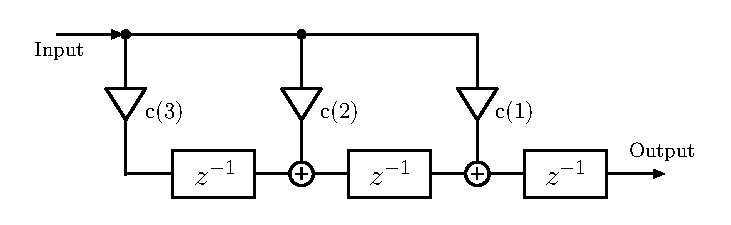
\includegraphics{fig/transflt.eps}
\end{center}
\begin{center}
(c)
\end{center}

\vspace{1mm}
\setlength{\unitlength}{0.9mm}
\begin{center}
\begin{picture}(80,20)(10,0)
  \thicklines
  \put(15,0){\framebox(32,16){$R_L(F_1(z))$}}
  \put(57,0){\framebox(32,16){$R_L(F_2(z))$}}
  \put(0,8){\vector(1,0){15}}
  \put(47,8){\vector(1,0){10}}
  \put(89,8){\vector(1,0){15}}
  \put(0,10){\makebox(0,0)[lb]{Input}}
  \put(91,10){\makebox(0,0)[lb]{Output}}
\end{picture}
\end{center}
\begin{center}
(d)
\end{center}

\caption{\protect\parbox[t]{8cm}{
	(a)~~$R_L(F(z))\simeq D(z)$~~~$L=4$ \protect\\
	(d)~~2 level cascade realization\protect\\
        \hspace*{5mm} $R_L(F_1(z))\cdot R_L(F_2(z))\simeq D(z)$
}}
\label{fig:lmadflt_LMA}

\end{figure}

\setcounter{table}{0}
\begin{table}
        \caption{The values for the coefficients $A_{L,l}$}
        \label{tbl:lmadflt_coef}
        \setlength{\arrayrulewidth}{0.5pt}
        \renewcommand{\arraystretch}{1.2}
        \begin{center}
        \begin{tabular}{|c|c|c|} \hline
        $l$     & $A_{4,l}$			& $A_{5,l}$ \\ \hline
        1       & $4.999273\times 10^{-1}$	& $4.999391\times 10^{-1}$\\
        2       & $1.067005\times 10^{-1}$      & $1.107098\times 10^{-1}$\\
        3       & $1.170221\times 10^{-2}$      & $1.369984\times 10^{-2}$\\
        4       & $5.656279\times 10^{-4}$      & $9.564853\times 10^{-4}$\\
        5       &                               & $3.041721\times 10^{-5}$\\
      \hline
        \end{tabular}
        \end{center}
\label{tbl:lmadflt_pade}
\end{table}

\end{qsection}


\begin{options}
	\argm{m}{M}{order of cepstrum}{25}
	\argm{p}{P}{frame period}{100}
	\argm{i}{I}{interpolation period}{1}
	\argm{P}{Pa}{order of the Pad\'e approximation\\
                     $Pa$ should be $4$ or $5$}{4}
	\argm{k}{}{filtering without gain}{FALSE}
	\argm{v}{}{inverse filter}{FALSE}
	\argm{t}{}{transpose filter}{FALSE}
        \desc[1ex]{(level 2)}
        \argm{B}{B1~B2~$\ldots$~Bn}{block size of cascaded filter,\\
        	                     where $(|B1|+\ldots+|Bn|)=m$}{FALSE}
\end{options}

\begin{qsection}{EXAMPLE}
In this example, the excitation is generated from
the pitch data read in float format from {\em data.pitch},
passed through an LMA filter obtained from cepstrum file
{\em data.cep}, and the synthesized speech is written to
{\em data.syn}.
\begin{quote}
 \verb!excite < data.pitch | lmadf -m 15 data.cep > data.syn!
\end{quote} 
If one wants to divide the filter into several blocks, the -B option
can be used to specify the block size of each filter.
For example, when dividing 15-dimentional filter into 3 sub-parts(4,
5, and 6), the corresponding command line is below.
\begin{quote}
 \verb!excite < data.pitch | lmadf -m 15 -B 4 5 6 data.cep > data.syn!
\end{quote}
If the block size value assigned by the -B option is negative, the
block is not used.
\begin{quote}
 \verb!excite < data.pitch | lmadf -m 15 -B 4 -5 6 data.cep > data.syn!
\end{quote}

\end{qsection}

\begin{qsection}{NOTICE}
$Pa$ = 4 or 5.\\
\end{qsection}

\begin{qsection}{SEE ALSO}
\hyperlink{uels}{uels},
\hyperlink{acep}{acep},
\hyperlink{poledf}{poledf},
\hyperlink{ltcdf}{ltcdf},
\hyperlink{glsadf}{glsadf},
\hyperlink{mlsadf}{mlsadf},
\hyperlink{mglsadf}{mglsadf}
\end{qsection}

%  ---------------------------------------------------------------  %
%            Speech Signal Processing Toolkit (SPTK)                %
%                      SPTK Working Group                           %
%                                                                   %
%                  Department of Computer Science                   %
%                  Nagoya Institute of Technology                   %
%                               and                                 %
%   Interdisciplinary Graduate School of Science and Engineering    %
%                  Tokyo Institute of Technology                    %
%                                                                   %
%                     Copyright (c) 1984-2007                       %
%                       All Rights Reserved.                        %
%                                                                   %
%  Permission is hereby granted, free of charge, to use and         %
%  distribute this software and its documentation without           %
%  restriction, including without limitation the rights to use,     %
%  copy, modify, merge, publish, distribute, sublicense, and/or     %
%  sell copies of this work, and to permit persons to whom this     %
%  work is furnished to do so, subject to the following conditions: %
%                                                                   %
%    1. The source code must retain the above copyright notice,     %
%       this list of conditions and the following disclaimer.       %
%                                                                   %
%    2. Any modifications to the source code must be clearly        %
%       marked as such.                                             %
%                                                                   %
%    3. Redistributions in binary form must reproduce the above     %
%       copyright notice, this list of conditions and the           %
%       following disclaimer in the documentation and/or other      %
%       materials provided with the distribution.  Otherwise, one   %
%       must contact the SPTK working group.                        %
%                                                                   %
%  NAGOYA INSTITUTE OF TECHNOLOGY, TOKYO INSTITUTE OF TECHNOLOGY,   %
%  SPTK WORKING GROUP, AND THE CONTRIBUTORS TO THIS WORK DISCLAIM   %
%  ALL WARRANTIES WITH REGARD TO THIS SOFTWARE, INCLUDING ALL       %
%  IMPLIED WARRANTIES OF MERCHANTABILITY AND FITNESS, IN NO EVENT   %
%  SHALL NAGOYA INSTITUTE OF TECHNOLOGY, TOKYO INSTITUTE OF         %
%  TECHNOLOGY, SPTK WORKING GROUP, NOR THE CONTRIBUTORS BE LIABLE   %
%  FOR ANY SPECIAL, INDIRECT OR CONSEQUENTIAL DAMAGES OR ANY        %
%  DAMAGES WHATSOEVER RESULTING FROM LOSS OF USE, DATA OR PROFITS,  %
%  WHETHER IN AN ACTION OF CONTRACT, NEGLIGENCE OR OTHER TORTUOUS   %
%  ACTION, ARISING OUT OF OR IN CONNECTION WITH THE USE OR          %
%  PERFORMANCE OF THIS SOFTWARE.                                    %
%                                                                   %
%  ---------------------------------------------------------------  %
%
\hypertarget{lpc}{}
\name{lpc}{LPC analysis using Levinson-Durbin method}{signal processing}

\begin{synopsis}
\item [lpc] [ --l $L$ ] [ --m $M$ ] [ {\em infile} ] 
\end{synopsis}

\begin{qsection}{DESCRIPTION}
{\em lpc} calculates linear prediction coefficients (LPC) 
from $L$-length framed windowed data from {\em infile} (or standard input), 
sending the result to standard output.

For each $L$-length input vector
\begin{displaymath}
  x(0),x(1),\ldots,x(L-1), 
\end{displaymath}
the autocorrelation function is calculated (see \hyperlink{acorr}{acorr}),
then the gain $K$ and the linear prediction coefficients 
$a(k) (1 \leq k \leq M)$ 
\begin{displaymath}
  K, a(1), \ldots, a(M)
\end{displaymath}
are calculated using the Levinson-Durbin algorithm. 

Input and output data are in float format.
\end{qsection}

\begin{options}
	\argm{l}{L}{frame length}{256}
	\argm{m}{M}{order of LPC}{25}
\end{options}

\begin{qsection}{EXAMPLE}
In this example, the 20-th order linear prediction analysis is applied
to input read from {\em data.f} in float format,
and the linear prediction coefficients are written to
{\em data.lpc}:
\begin{quote}
 \verb!frame +f < data.f | window | lpc -m 20 > data.lpc!
\end{quote} 
\end{qsection}

\begin{qsection}{SEE ALSO}
\hyperlink{acorr}{acorr},
\hyperlink{levdur}{levdur},
\hyperlink{lpc2par}{lpc2par},
\hyperlink{par2lpc}{par2lpc},
\hyperlink{lpc2c}{lpc2c},
\hyperlink{lpc2lsp}{lpc2lsp},
\hyperlink{lsp2lpc}{lsp2lpc}
\hyperlink{ltcdf}{ltcdf},
\hyperlink{lspdf}{lspdf}
\end{qsection}

% ----------------------------------------------------------------
%       Speech Signal Processing Toolkit (SPTK): version 3.0
%                      SPTK Working Group
% 
%                Department of Computer Science
%                Nagoya Institute of Technology
%                             and
%   Interdisciplinary Graduate School of Science and Engineering
%                Tokyo Institute of Technology
%                   Copyright (c) 1984-2000
%                     All Rights Reserved.
% 
% Permission is hereby granted, free of charge, to use and
% distribute this software and its documentation without
% restriction, including without limitation the rights to use,
% copy, modify, merge, publish, distribute, sublicense, and/or
% sell copies of this work, and to permit persons to whom this
% work is furnished to do so, subject to the following conditions:
% 
%   1. The code must retain the above copyright notice, this list
%      of conditions and the following disclaimer.
% 
%   2. Any modifications must be clearly marked as such.
%                                                                        
% NAGOYA INSTITUTE OF TECHNOLOGY, TOKYO INSITITUTE OF TECHNOLOGY,
% SPTK WORKING GROUP, AND THE CONTRIBUTORS TO THIS WORK DISCLAIM
% ALL WARRANTIES WITH REGARD TO THIS SOFTWARE, INCLUDING ALL
% IMPLIED WARRANTIES OF MERCHANTABILITY AND FITNESS, IN NO EVENT
% SHALL NAGOYA INSTITUTE OF TECHNOLOGY, TOKYO INSITITUTE OF
% TECHNOLOGY, SPTK WORKING GROUP, NOR THE CONTRIBUTORS BE LIABLE
% FOR ANY SPECIAL, INDIRECT OR CONSEQUENTIAL DAMAGES OR ANY
% DAMAGES WHATSOEVER RESULTING FROM LOSS OF USE, DATA OR PROFITS,
% WHETHER IN AN ACTION OF CONTRACT, NEGLIGENCE OR OTHER TORTIOUS
% ACTION, ARISING OUT OF OR IN CONNECTION WITH THE USE OR
% PERFORMANCE OF THIS SOFTWARE.
% ----------------------------------------------------------------
%
\name{lpc2c}{LPC$B%1%W%9%H%i%`(B}{$B2;@<%Q%i%a!<%?JQ49(B}

\begin{synopsis}
 \item[lpc2c] [ --m $M_1$ ] [ --M $M_2$ ] [ {\em infile} ]
\end{synopsis}
\begin{qsection}{DESCRIPTION}
{\em lpc2c} $B$O!$;XDj$5$l$?%U%!%$%k$+$i(BLPC$B78?t$rFI$_(B
$B9~$_!$(BLPC$B%1%W%9%H%i%`$r=PNO$7$^$9!%(B
$B$D$^$j!$F~NO?tNs$r(B
\[ \sigma, a(1), a(2), \cdots, a(p) \]
$B$H$7$F!$(B
\[
c(n) =\left\{
\begin{array}{lc}
 ln(h),&n=0\\
\displaystyle -a(n)=-\sum^{n-1}_{k=1}\frac{k}{n}c(k) a(n-k),&1\leq n\leq P\\
\displaystyle -\sum_{k=n-P}^{n-1}\frac{k}{n}c(k) a(n-k),& n>P
\end{array}
\right.
\]
$BC"$7!$(B
\[
H(z)=\frac{\sigma}{A(z)}=\frac{\sigma}{\displaystyle 1+\sum_{k=1}^P a(k) z^{-k}}
\]
$B$r7W;;$7!$(B
\[ c(0), c(1), \cdots, c(M) \]
$B$r=PNO$7$^$9!%(B
$B%G!<%?7A<0$OF~=PNO$H$b(B float $B7A<0$G$9!%(B
\end{qsection}

\begin{options}
	\argm{m}{M_1}{LPC $B$N<!?t!%(B}{25}
	\argm{M}{M_2}{$B%1%W%9%H%i%`$N<!?t!%(B}{25}
\end{options}

\begin{qsection}{EXAMPLE}
float$B7A<0$N2;@<%G!<%?(B {\em data.f} $B$KAk3]$1$7$?%G!<%?$N(B10$B<!$N(B
LPC$B78?t$r5a$a!$$5$i$K(B15$B<!$N(BLPC$B%1%W%9%H%i%`$r5a$a!$(B{\em data.cep} $B$K=PNO$9$k(B:
\begin{quote}
 \verb!frame < data.f | window | lpc -m 10 |\!\\
 \verb!lpc2c -m 10 -M 15 > data.cep!
\end{quote}
\end{qsection}

\begin{qsection}{SEE ALSO}
lpc, gc2gc, mgc2mgc, freqt
\end{qsection}

%  ---------------------------------------------------------------  %
%            Speech Signal Processing Toolkit (SPTK)                %
%                      SPTK Working Group                           %
%                                                                   %
%                  Department of Computer Science                   %
%                  Nagoya Institute of Technology                   %
%                               and                                 %
%   Interdisciplinary Graduate School of Science and Engineering    %
%                  Tokyo Institute of Technology                    %
%                                                                   %
%                     Copyright (c) 1984-2007                       %
%                       All Rights Reserved.                        %
%                                                                   %
%  Permission is hereby granted, free of charge, to use and         %
%  distribute this software and its documentation without           %
%  restriction, including without limitation the rights to use,     %
%  copy, modify, merge, publish, distribute, sublicense, and/or     %
%  sell copies of this work, and to permit persons to whom this     %
%  work is furnished to do so, subject to the following conditions: %
%                                                                   %
%    1. The source code must retain the above copyright notice,     %
%       this list of conditions and the following disclaimer.       %
%                                                                   %
%    2. Any modifications to the source code must be clearly        %
%       marked as such.                                             %
%                                                                   %
%    3. Redistributions in binary form must reproduce the above     %
%       copyright notice, this list of conditions and the           %
%       following disclaimer in the documentation and/or other      %
%       materials provided with the distribution.  Otherwise, one   %
%       must contact the SPTK working group.                        %
%                                                                   %
%  NAGOYA INSTITUTE OF TECHNOLOGY, TOKYO INSTITUTE OF TECHNOLOGY,   %
%  SPTK WORKING GROUP, AND THE CONTRIBUTORS TO THIS WORK DISCLAIM   %
%  ALL WARRANTIES WITH REGARD TO THIS SOFTWARE, INCLUDING ALL       %
%  IMPLIED WARRANTIES OF MERCHANTABILITY AND FITNESS, IN NO EVENT   %
%  SHALL NAGOYA INSTITUTE OF TECHNOLOGY, TOKYO INSTITUTE OF         %
%  TECHNOLOGY, SPTK WORKING GROUP, NOR THE CONTRIBUTORS BE LIABLE   %
%  FOR ANY SPECIAL, INDIRECT OR CONSEQUENTIAL DAMAGES OR ANY        %
%  DAMAGES WHATSOEVER RESULTING FROM LOSS OF USE, DATA OR PROFITS,  %
%  WHETHER IN AN ACTION OF CONTRACT, NEGLIGENCE OR OTHER TORTUOUS   %
%  ACTION, ARISING OUT OF OR IN CONNECTION WITH THE USE OR          %
%  PERFORMANCE OF THIS SOFTWARE.                                    %
%                                                                   %
%  ---------------------------------------------------------------  %
%
\hypertarget{lpc2lsp}{}
\name{lpc2lsp}{transform LPC to LSP}{speech parameter transformation}

\begin{synopsis}
\item [lpc2lsp] [ --m $M$ ] [ --s $S$ ] [ --k ] [ --l ] [ --o $O$ ] [ --n $N$ ]
		[ --p $P$ ] [ --q $Q$ ] [ --d $D$ ] 
\item [\ ~~~~~~~~] [ {\em infile} ] 
\end{synopsis}

\begin{qsection}{DESCRIPTION}
{\em lpc2lsp} calculates line spectral pair (LSP) coefficients 
from $M$-th order linear prediction (LPC) coefficients 
from {\em infile} (or standard input),
sending the result to standard output.

The gain $K$ is included in the LPC input vectors
\begin{displaymath}
  K, a(1), \dots, a(M)
\end{displaymath}
but $K$ is not used in the calculation of the LSP coefficients.

The $M$-th order polynomial linear prediction equation $A(z)$ is
\begin{displaymath}
  A_M(z) = 1 + \sum_{m=1}^M a(m) z^{-m}
\end{displaymath}
The PARCOR coefficients satisfy the following equations.
\begin{align}
  A_m(z) &= A_{m-1}(z) - k(m) B_{m-1}(z) \notag \\
  B_m(z) &= z^{-1} (B_{m-1}(z) - k(m) A_{m-1}(z)) \notag
\end{align}
Also, the initial conditions are set as follows,
\begin{displaymath}
  A_0(z) = 1, \qquad B_0(z) = z^{-1}
\end{displaymath}
When we are given the linear prediction polynomial equation
of $M$-th order $A_M(z)$, and when the evaluation of $A_{M+1}(z)$
is obtained with the value of $k(M+1)$ equal to $1$ or $-1$, 
$P(z)$ and $Q(z)$ are defined as follow.
\begin{align}
  P(z) &= A_M(z) - B_M(z) \notag \\
  Q(z) &= A_M(z) + B_M(z) \notag
\end{align}
Making $k(M+1)$ equal to $\pm 1$ is means that,
with respect PARCOR coefficients,
the boundary condition for the glottis of the fixed vocal tract model
satisfies a perfect reflection characteristic.
Also, $A_M(z)$ can be expressed as
\begin{displaymath}
  A_M(z) = ( P(z) + Q(z) ) / 2.
\end{displaymath}
When we express $A_M(z)$ in this way,
$A_M(z)$ is stable.
That is for the roots of $A_M(z)=0$ to be all inside
the unit circle a necessary and sufficient condition is given
in the following.
\begin{itemize}
\item All of the roots of $P(z)=0$ and $Q(z)=0$ are on the unit circle
      line.
\item the roots of $P(z)=0$ and $Q(z)=0$ should be above the unit
      circle line and intercalate.
\end{itemize}
In other words, if  the roots of $P(z)=0$ and $Q(z)=0$ satisfy the
above condition, then $A_M(z)$ is stable.
\par
If we assume that $M$ is a even number, then
$P(z)$ and $Q(z)$ can be factorized as follows.
\begin{align}
  P(z) &= ( 1 - z^{-1} ) \prod_{i=2,4,\dots,M}
          ( 1 - 2 z^{-1} \cos \omega_i + z^{-2} ) \notag \\
  Q(z) &= ( 1 + z^{-1} ) \prod_{i=1,3,\dots,M-1}
          ( 1 - 2 z^{-1} \cos \omega_i + z^{-2} ) \notag
\end{align}
Also, the values of $\omega_i$ satisfy the following ordering condition.
\begin{displaymath}
  0 < \omega_1 < \omega_2 < \dots < \omega_{M-1} < \omega_M < \pi
\end{displaymath}
In the case, $M$ is odd number solution can be found in a similar way.
The coefficients $\omega_i$ obtained through factorization are called
LSP coefficients.
\end{qsection}

\begin{options}
	\argm{m}{M}{order of LPC}{25}
	\argm{s}{S}{sampling frequency (kHz)}{10}
	\argm{k}{}{output gain}{TRUE}
	\argm{l}{}{output log gain instead of linear gain}{FALSE}
	\argm{o}{O}{output format \\
		\begin{tabular}{ll} \\[-1ex]
			$0$ & normalized frequency $(0 \dots \pi)$ \\
			$1$ & normalized frequency $(0 \dots 0.5)$ \\
			$2$ & frequency (kHz) \\
			$3$ & frequency (Hz)  \\
		\end{tabular}\\\hspace*{\fill}}{0}
	\desc[0.6ex]{Usually, the options below do not need to be assigned.}
	\argm{n}{N}{split number of unit circle}{128}
	\argm{p}{P}{maximum number of interpolation for $P(z)$}{4}
	\argm{q}{Q}{maximum number of interpolation for $Q(z)$}{15}
	\argm{d}{D}{end condition of interpolation}{1e-06}
\end{options}

\begin{qsection}{EXAMPLE}
In the following example, speech data is read in float format from
{\em data.f}, 10-th order LPC coefficients are calculated,
and the LSP coefficients are evaluated and written to {\em data.lsp}:
\begin{quote}
\verb!frame < data.f | window | lpc -m 10 |\!\\
\verb!lpc2lsp -m 10 > data.lsp!
\end{quote}
\end{qsection}

\begin{qsection}{SEE ALSO}
\hyperlink{lpc}{lpc},
\hyperlink{lsp2lpc}{lsp2lpc},
\hyperlink{lspdf}{lspdf}
\end{qsection}

\name{lpc2par}{$B@~7AM=B,78?t$+$iH?<M78?t$r5a$a$k(B}

\begin{synopsis}
\item [lpc2par] [ --m $M$ ] [ --g $G$ ] [ --s ] [ {\em infile} ] 
\end{synopsis}

\begin{qsection}{DESCRIPTION}
$B@~7AM=B,78?t$+$iH?<M78?t(B(PARCOR)$B$r5a$a$^$9!%(B
$B;XDj$5$l$?%U%!%$%k$+$i(B $M$ $B<!$N@~7AM=B,78?t(B
\begin{displaymath}
  K, a(1),\ldots, a(M)
\end{displaymath}
$B$rFI$_9~$_!$H?<M78?t(B
\begin{displaymath}
  K, k(1),\ldots, k(M)
\end{displaymath}
$B$rI8=`=PNO$K=PNO$7$^$9!%(B
$B$^$?!$(B --s $B%*%W%7%g%s$r;XDj$7$?>l9g$K$O!$0BDj@-$NH=JL$r9T$$!$0BDj$N>l9g$K$O(B
0$B!$IT0BDj$N>l9g$K$O(B1$B$,I8=`=PNO$K=PNO$5$l$^$9!%(B
\par
$B%G!<%?7A<0$OF~NO!$=PNO$H$b(Bfloat $B7A<0$G$9!%(B
\par
$B@~7AM=B,78?t$+$iH?<M78?t$r5a$a$kJQ49$O!$(B
\begin{eqnarray*} 
k(m) &=& a^{(m)}(m) \\
a^{(m-1)}(i) &=& \frac{a^{(m)}(i)+a^{(m)}(m)a^{(m)}(m-i)}{1-k^2(m)},
~~~~~1 \leq i \leq m-1
\end{eqnarray*}
$B$r(B $m=p, p-1, \ldots, 1$ $B$N=g$K7+$jJV$7$^$9!%$3$3$G!$=i4|>r7o$O(B
\begin{displaymath}
a^{(M)}(m) = a(m), ~~~~~1 \leq m \leq M
\end{displaymath}
$B$G$9!%(B
--g$B%*%W%7%g%s$r;XDj$7$?>l9g!$$Y$-%Q%i%a!<%?$r(B$\gamma$$B$H$9$k(B
$B@55,2=0lHL2=%1%W%9%H%i%`$rF~NO$H$7$F!$H?<M78?t$r5a$a$^$9!%(B
$B$3$N>l9gF~NO(B
\begin{displaymath}
K,c_\gamma'(1),\ldots,c_\gamma'(M)
\end{displaymath}
$B$rFI$_9~$_!$(B
\begin{displaymath}
a^{(M)}(m) = \gamma c_\gamma'(M), ~~~~~1 \leq m \leq M
\end{displaymath}
$B$H$7$F!$7W;;$7$^$9!%(B

$B$^$?!$0BDj@-$NH=JL$9$k:]$K$O!$H?<M78?t$,$9$Y$F(B
\begin{displaymath}
-1 < k(m) < 1
\end{displaymath}
$B$H$$$&>r7o$rK~$?$7$F$$$k$+D4$Y$F$$$^$9!%(B

\end{qsection}

\newpage
\begin{options}
	\argm{m}{M}{LPC$B$N<!?t!%(B}{25}
	\argm{g}{G}{$B0lHL2=%1%W%9%H%i%`$N$Y$-%Q%i%a!<%?(B $\gamma$$B!%(B\\
			 $B$?$@$7!$(B$G>1.0$ $B$N$H$-$O(B $\gamma=-1/G$$B!%(B}{1}
	\argm{s}{}{$B0BDj@-$rH=JL$7!$0BDj$J$i$P(B0$B!$IT0BDj$J$i$P(B1$B$r=PNO!%(B}{FALSE}
\end{options}

\begin{qsection}{EXAMPLE}
float$B7A<0$N%U%!%$%k(B {\em data.f} $B$r@~7AM=B,J,@O$7!$@~7AM=B,78?t$r(B
$BH?<M78?t$KJQ49$7!$(B{\em data.rc} $B$K=PNO$9$k(B:
\begin{quote}
 \verb!frame < data.f | window | lpc | lpc2par > data.rc!
\end{quote} 
\end{qsection}

\begin{qsection}{SEE ALSO}
 acorr, levdur, lpc, par2lpc, ltcdf
\end{qsection}

\name{lsp2lpc}{LSP $B$+$i(B LPC $B$KJQ49(B}{none}

\begin{synopsis}
\item [lsp2lpc] [ --m $M$ ] [ --s $S$ ] [ --k ] [ --i $I$ ] [ {\em infile} ] 
\end{synopsis}

\begin{qsection}{DESCRIPTION}
 {\em lsp2lpc}$B$O!$(Blsp $B78?t$r@~7AM=B,78?t$KJQ49$7$^$9!%(B
 $B%2%$%s9`$rF~=PNO$7$J$$>l9g$O%2%$%s9`$r(B1$B$H$7$?(BLPC$B78?t(B
\begin{displaymath}
	K = 1,a(1),\ldots,a(M)
 \end{displaymath}
$B$r=PNO$7$^$9!%(B
\end{qsection}

\begin{options}
	\argm{m}{M}{LPC $B$N<!?t!%(B}{25}
	\argm{s}{S}{$B%5%s%W%j%s%0<~GH?t(B (kHz)$B!%(B}{10}
	\argm{k}{}{$B%2%$%s$NF~=PNO(B}{TRUE}
	\argm{i}{I}{$BF~NO7A<0!%(B \\
		\begin{tabular}{ll} \\[-1zh]
			$0$ & $B5,3J2=<~GH?t(B $(0 \ldots \pi)$ \\
			$1$ & $B5,3J2=<~GH?t(B $(0 \ldots 0.5)$ \\
			$2$ & $B<~GH?t(B (kHz) \\
			$3$ & $B<~GH?t(B (Hz)  \\
		\end{tabular}\\\hspace*{\fill}}{0}
\end{options}

\begin{qsection}{EXAMPLE}
float$B7A<0$N(B10$B<!$N(Blsp$B78?t%U%!%$%k(B{\em data.lsp}$B$+$i@~7AM=B,78?t$r5a$a!$(B
{\em data.lpc} $B$K=PNO$9$k(B:
\begin{quote}
\verb! lsp2lpc -m 10 < data.lsp > data.lpc!
\end{quote}
\end{qsection}

\begin{qsection}{SEE ALSO}
lpc, lpc2lsp
\end{qsection}

% ----------------------------------------------------------------- %
%             The Speech Signal Processing Toolkit (SPTK)           %
%             developed by SPTK Working Group                       %
%             http://sp-tk.sourceforge.net/                         %
% ----------------------------------------------------------------- %
%                                                                   %
%  Copyright (c) 1984-2007  Tokyo Institute of Technology           %
%                           Interdisciplinary Graduate School of    %
%                           Science and Engineering                 %
%                                                                   %
%                1996-2015  Nagoya Institute of Technology          %
%                           Department of Computer Science          %
%                                                                   %
% All rights reserved.                                              %
%                                                                   %
% Redistribution and use in source and binary forms, with or        %
% without modification, are permitted provided that the following   %
% conditions are met:                                               %
%                                                                   %
% - Redistributions of source code must retain the above copyright  %
%   notice, this list of conditions and the following disclaimer.   %
% - Redistributions in binary form must reproduce the above         %
%   copyright notice, this list of conditions and the following     %
%   disclaimer in the documentation and/or other materials provided %
%   with the distribution.                                          %
% - Neither the name of the SPTK working group nor the names of its %
%   contributors may be used to endorse or promote products derived %
%   from this software without specific prior written permission.   %
%                                                                   %
% THIS SOFTWARE IS PROVIDED BY THE COPYRIGHT HOLDERS AND            %
% CONTRIBUTORS "AS IS" AND ANY EXPRESS OR IMPLIED WARRANTIES,       %
% INCLUDING, BUT NOT LIMITED TO, THE IMPLIED WARRANTIES OF          %
% MERCHANTABILITY AND FITNESS FOR A PARTICULAR PURPOSE ARE          %
% DISCLAIMED. IN NO EVENT SHALL THE COPYRIGHT OWNER OR CONTRIBUTORS %
% BE LIABLE FOR ANY DIRECT, INDIRECT, INCIDENTAL, SPECIAL,          %
% EXEMPLARY, OR CONSEQUENTIAL DAMAGES (INCLUDING, BUT NOT LIMITED   %
% TO, PROCUREMENT OF SUBSTITUTE GOODS OR SERVICES; LOSS OF USE,     %
% DATA, OR PROFITS; OR BUSINESS INTERRUPTION) HOWEVER CAUSED AND ON %
% ANY THEORY OF LIABILITY, WHETHER IN CONTRACT, STRICT LIABILITY,   %
% OR TORT (INCLUDING NEGLIGENCE OR OTHERWISE) ARISING IN ANY WAY    %
% OUT OF THE USE OF THIS SOFTWARE, EVEN IF ADVISED OF THE           %
% POSSIBILITY OF SUCH DAMAGE.                                       %
% ----------------------------------------------------------------- %
\hypertarget{lsp2sp}{}
\name{lsp2sp}{transform LSP to spectrum}
{speech parameter transformation}

\begin{synopsis}
\item[lsp2sp] [ --m $M$ ] [ --s $S$ ] [ --l $L$ ] [ --L ] [ --k ] [ --q $Q$ ] [ --o $O$ ] [ {\em infile} ]
\end{synopsis}

\begin{qsection}{DESCRIPTION}
{\em lsp2sp} calculates the spectrum from the line spectral pairs (LSP)
from {\em infile} (or standard input),
sending the result to standard output.

Input and output data are in float format.

The LSP input format is
 \begin{displaymath}
  [ K ], l(1), \dots, l(M).
 \end{displaymath}
The spectrum can be obtained by
  \begin{displaymath}
   \mid H(\mathrm{e}^{-j\omega}) \mid = \frac{K}{\mid A_p(\mathrm{e}^{-j\omega}) \mid}.
  \end{displaymath}
where $\mid A_p(\mathrm{e}^{-j\omega}) \mid$ is given as follows:

When the order of LSP is even, 
  \begin{displaymath}
   \mid A_p(\mathrm{e}^{-j\omega}) \mid = \sqrt{ 2^M \left\{ \cos^2 \frac{\omega}{2}\prod_{i=1,3,\cdots,M-1}(\cos \omega - \cos l(i))^2 + \sin^2 \frac{\omega}{2}\prod_{i=2,4,\cdots,M}(\cos \omega - \cos l(i))^2 \right\} }.
  \end{displaymath}
When the order of LSP is odd,
 \begin{displaymath}
  \mid A_p(\mathrm{e}^{-j\omega}) \mid = \sqrt{ 2^{M-1} \left\{ \prod_{i=1,3,\cdots,M}(\cos \omega - \cos l(i))^2 + \sin^2 \omega \prod_{i=2,4,\cdots,M-1}(\cos \omega - \cos l(i))^2 \right\} }.
 \end{displaymath}
\end{qsection}

\begin{options}
 \argm{m}{M}{order of LSP}{10}
 \argm{s}{S}{sampling frequency (kHz)}{10.0}
	\argm{l}{L}{frame length}{256}
 \argm{L}{}{regard input log gain as linear one}{FALSE}
	\argm{q}{Q}{input format\\
        \begin{tabular}{ll} \\[-1ex]
            $0$ & normalized frequency $(0 \dots \pi)$ \\
            $1$ & normalized frequency $(0 \dots 0.5)$ \\
            $2$ & frequency (kHz) \\
            $3$ & frequency (Hz)  \\
        \end{tabular}\\\hspace*{\fill}}{0}
	\argm{o}{O}{output format\\
 \begin{tabular}{ll} \\[-1ex]
  $0$ & $20 \times \log |H(z)|$ \\
  $1$ & $\ln |H(z)|$ \\
  $2$ & $|H(z)|$ \\
  $3$ & $|H(z)|^{2}$ \\[1ex]
 \end{tabular}\\\hspace*{\fill}}{0}
\end{options}

\begin{qsection}{EXAMPLE}
The example below takes the 15-th order LSP from the file
 {\em data.cep} in float format, evaluates the spectrum,
 and presents it in the screen:
\begin{quote}
 \verb! lsp2sp -m 15 data.lsp | glogsp | xgr ! 
\end{quote}
\end{qsection}

\begin{qsection}{SEE ALSO}
\hyperlink{lpc2lsp}{lpc2lsp},
\hyperlink{lspcheck}{lspcheck}
\end{qsection}

% ----------------------------------------------------------------- %
%             The Speech Signal Processing Toolkit (SPTK)           %
%             developed by SPTK Working Group                       %
%             http://sp-tk.sourceforge.net/                         %
% ----------------------------------------------------------------- %
%                                                                   %
%  Copyright (c) 1984-2007  Tokyo Institute of Technology           %
%                           Interdisciplinary Graduate School of    %
%                           Science and Engineering                 %
%                                                                   %
%                1996-2013  Nagoya Institute of Technology          %
%                           Department of Computer Science          %
%                                                                   %
% All rights reserved.                                              %
%                                                                   %
% Redistribution and use in source and binary forms, with or        %
% without modification, are permitted provided that the following   %
% conditions are met:                                               %
%                                                                   %
% - Redistributions of source code must retain the above copyright  %
%   notice, this list of conditions and the following disclaimer.   %
% - Redistributions in binary form must reproduce the above         %
%   copyright notice, this list of conditions and the following     %
%   disclaimer in the documentation and/or other materials provided %
%   with the distribution.                                          %
% - Neither the name of the SPTK working group nor the names of its %
%   contributors may be used to endorse or promote products derived %
%   from this software without specific prior written permission.   %
%                                                                   %
% THIS SOFTWARE IS PROVIDED BY THE COPYRIGHT HOLDERS AND            %
% CONTRIBUTORS "AS IS" AND ANY EXPRESS OR IMPLIED WARRANTIES,       %
% INCLUDING, BUT NOT LIMITED TO, THE IMPLIED WARRANTIES OF          %
% MERCHANTABILITY AND FITNESS FOR A PARTICULAR PURPOSE ARE          %
% DISCLAIMED. IN NO EVENT SHALL THE COPYRIGHT OWNER OR CONTRIBUTORS %
% BE LIABLE FOR ANY DIRECT, INDIRECT, INCIDENTAL, SPECIAL,          %
% EXEMPLARY, OR CONSEQUENTIAL DAMAGES (INCLUDING, BUT NOT LIMITED   %
% TO, PROCUREMENT OF SUBSTITUTE GOODS OR SERVICES; LOSS OF USE,     %
% DATA, OR PROFITS; OR BUSINESS INTERRUPTION) HOWEVER CAUSED AND ON %
% ANY THEORY OF LIABILITY, WHETHER IN CONTRACT, STRICT LIABILITY,   %
% OR TORT (INCLUDING NEGLIGENCE OR OTHERWISE) ARISING IN ANY WAY    %
% OUT OF THE USE OF THIS SOFTWARE, EVEN IF ADVISED OF THE           %
% POSSIBILITY OF SUCH DAMAGE.                                       %
% ----------------------------------------------------------------- %
\hypertarget{lspcheck}{}
\name{lspcheck}{check stability and rearrange LSP}{speech parameter transformation}

\begin{synopsis}
\item [lspcheck] [ --m $M$ ] [ --s $S$ ] [ --k ] [ --L ] [ --i $I$ ] [ --o $O$ ]
		[ --r $R$] [ --G $G$ ] [ --g ] [ {\em infile} ]
\end{synopsis}

\begin{qsection}{DESCRIPTION}
{\em lspcheck} tests the stability of the filter 
corresponding to the line spectral pair (LSP) coefficients 
from {\em infile} (or standard input), 
sending the result to standard output.

By default, the output is the same as the input.
When the --c option is given,
the output is LSP coefficients
that have been rearranged so the filter is stable.
If an frame is unstable, an ASCII report of the number of the frame
is sent to standard error.
\end{qsection}

\begin{options}
	\argm{m}{M}{order of LPC}{25}
	\argm{s}{S}{sampling frequency (kHz)}{10.0}
	\argm{k}{}{input \& output gain}{TRUE}
    \argm{L}{}{regard input as log gain}{FALSE}
	\argm{i}{I}{input format}{0}
	\argm{o}{O}{output format \\
		\begin{tabular}{ll} \\[-1ex]
			$0$ & normalized frequency $(0 \ldots \pi)$ \\
			$1$ & normalized frequency $(0 \ldots 0.5)$ \\
			$2$ & frequency (kHz) \\
			$3$ & frequency (Hz)  \\
		\end{tabular}\\\hspace*{\fill}}{$I$}
	\argm{c}{}{rearrange LSP\\
check the distance between two consecutive LSPs\\
and extend the distance (if it is smaller than $R\times \pi/M$)}{N/A}
	\argm{r}{R}{threshold of rearrangement of LSP\\
    $s.t.\hspace{0.5cm} 0 \leq R \leq 1$}{0.0}
    \argm{G}{G}{minimum value of gain\\
                $G$ must be greater than $0$.}{1e-10}
    \argm{g}{}{modify gain value if gain is less than $G$.}{FALSE}
\end{options}

\begin{qsection}{EXAMPLE}
In the following example, 10-th order LSP coefficients are
read from {\em data.lsp} in float format,
stability is checked, the unstable coefficients are rearranged
so that they become stable, and the distance between two
consecutive LSPs are extended to $\pi /1000$ if
 it is smaller than $\pi /1000$, and the
 rearranged LSP coefficients are written to {\em data.lspr}:
\begin{quote}
\verb!lspcheck -m 10 -c -r 0.01 < data.lsp > data.lspr!
\end{quote}
\end{qsection}

\begin{qsection}{SEE ALSO}
\hyperlink{lpc}{lpc},
\hyperlink{lpc2lsp}{lpc2lsp},
\hyperlink{lsp2lpc}{lsp2lpc}
\end{qsection}

% ----------------------------------------------------------------
%       Speech Signal Processing Toolkit (SPTK): version 3.0
%                      SPTK Working Group
% 
%                Department of Computer Science
%                Nagoya Institute of Technology
%                             and
%   Interdisciplinary Graduate School of Science and Engineering
%                Tokyo Institute of Technology
%                   Copyright (c) 1984-2000
%                     All Rights Reserved.
% 
% Permission is hereby granted, free of charge, to use and
% distribute this software and its documentation without
% restriction, including without limitation the rights to use,
% copy, modify, merge, publish, distribute, sublicense, and/or
% sell copies of this work, and to permit persons to whom this
% work is furnished to do so, subject to the following conditions:
% 
%   1. The code must retain the above copyright notice, this list
%      of conditions and the following disclaimer.
% 
%   2. Any modifications must be clearly marked as such.
%                                                                        
% NAGOYA INSTITUTE OF TECHNOLOGY, TOKYO INSITITUTE OF TECHNOLOGY,
% SPTK WORKING GROUP, AND THE CONTRIBUTORS TO THIS WORK DISCLAIM
% ALL WARRANTIES WITH REGARD TO THIS SOFTWARE, INCLUDING ALL
% IMPLIED WARRANTIES OF MERCHANTABILITY AND FITNESS, IN NO EVENT
% SHALL NAGOYA INSTITUTE OF TECHNOLOGY, TOKYO INSITITUTE OF
% TECHNOLOGY, SPTK WORKING GROUP, NOR THE CONTRIBUTORS BE LIABLE
% FOR ANY SPECIAL, INDIRECT OR CONSEQUENTIAL DAMAGES OR ANY
% DAMAGES WHATSOEVER RESULTING FROM LOSS OF USE, DATA OR PROFITS,
% WHETHER IN AN ACTION OF CONTRACT, NEGLIGENCE OR OTHER TORTIOUS
% ACTION, ARISING OUT OF OR IN CONNECTION WITH THE USE OR
% PERFORMANCE OF THIS SOFTWARE.
% ----------------------------------------------------------------
%
\name{lspdf}{$B2;@<9g@.$N$?$a$N(BLSP $B%G%#%8%?%k%U%#%k%?(B}%
{$B2;@<9g@.MQ%U%#%k%?(B}

\begin{synopsis}
\item [lspdf] [ --m $M$ ] [ --p $P$ ] [ --i $I$ ] [ --s $S$ ] [ --o $O$ ] 
              [ --k ] {\em lspfile} [ {\em infile} ] 
\end{synopsis}

\begin{qsection}{DESCRIPTION}
 {\em lspdf}$B$O!$F~NO%G!<%?$r(B{\em lspfile}$B$N(B lsp $B78?t(B
$K, f(1),\ldots,f(M)$ $B$r$b$D(B lsp $B9g@.%U%#%k%?(B
$B$K$h$j%U%#%k%?%j%s%0$7!$I8=`=PNO$K=PNO$7$^$9!%(B
\par
$B%G!<%?7A<0$OF~NO!$=PNO$H$b(Bfloat $B7A<0$G$9!%(B
\end{qsection}

\begin{options}
	\argm{m}{M}{lsp$B78?t$N<!?t!%(B}{25}
	\argm{p}{P}{$B%U%l!<%`<~4|(B}{100}
	\argm{i}{I}{$BJd4V<~4|!%(B}{1}
	\argm{s}{S}{$B%5%s%W%j%s%0<~GH?t(B (kHz).}{10}
	\argm{o}{O}{$BF~NO7A<0!%(B \\
		\begin{tabular}{ll} \\[-1zh]
			$0$ & $B5,3J2=<~GH?t(B $(0 \ldots \pi)$ \\
			$1$ & $B5,3J2=<~GH?t(B $(0 \ldots 0.5)$ \\
			$2$ & $B<~GH?t(B (kHz) \\
			$3$ & $B<~GH?t(B (Hz)  \\
		\end{tabular}\\\hspace*{\fill}}{0}
	\argm{k}{}{$B%2%$%s$r=|$$$?%7%9%F%`4X?t$G%U%#%k%?%j%s%0$9$k(B}{FALSE}
\end{options}

\begin{qsection}{EXAMPLE}
float$B7A<0$N%T%C%A%G!<%?(B {\em data.pitch} $B$+$iNe?68;$r:n@.$7!$(B
lsp$B%U%!%$%k(B {\em data.lsp} $B$K$h$j(Blsp$B9g@.%U%#%k%?$r6nF0$7!$(B
$B9g@.2;@<$r(B {\em data.syn} $B$K=PNO$9$k(B:
\begin{quote}
\verb! excite < data.pitch | lspdf data.lsp > data.syn!
\end{quote}
\end{qsection}

\begin{qsection}{SEE ALSO}
 lps, lpc2lsp
\end{qsection}

\name{ltcdf}{all-pole lattice digital filter for speech synthesis}%
{filters for speech synthesis}

\begin{synopsis}
\item [ltcdf] [ --m $M$ ] [ --p $P$ ] [ --i $I$ ] [ --k ] {\em rcfile} 
	      [ {\em infile} ] 
\end{synopsis}

\begin{qsection}{DESCRIPTION}
The {\em ltcdf} command reads excitation information from
{\em infile},  passes it through a lattice filter
obtained from the PARCOR coefficients read from {\em rcfile},
and sends the results to the standard output.
\par
Input and output data are in float format.
\end{qsection}

\begin{options}
	\argm{m}{M}{order of coefficients}{25}
	\argm{p}{P}{frame period}{100}
	\argm{i}{I}{interpolation period}{1}
	\argm{k}{}{filtering without gain}{FALSE}
\end{options}

\begin{qsection}{EXAMPLE}
In the example below, excitation is generated from
pitch information given in {\em data.pitch} in float format,
this excitation is passed through the lattice filter
constructed from the LPC file {\em data.rc},
and the synthesized speech is written to {\em data.syn}:
\begin{quote}
 \verb!excite < data.pitch | ltcdf data.k > data.syn!
\end{quote} 
\end{qsection}

\begin{qsection}{SEE ALSO}
 lpc, acorr, levdur, lpc2par, par2lpc, poledf, zerodf, lspdf
\end{qsection}

% ----------------------------------------------------------------
%       Speech Signal Processing Toolkit (SPTK): version 3.0
%                      SPTK Working Group
% 
%                Department of Computer Science
%                Nagoya Institute of Technology
%                             and
%   Interdisciplinary Graduate School of Science and Engineering
%                Tokyo Institute of Technology
%                   Copyright (c) 1984-2000
%                     All Rights Reserved.
% 
% Permission is hereby granted, free of charge, to use and
% distribute this software and its documentation without
% restriction, including without limitation the rights to use,
% copy, modify, merge, publish, distribute, sublicense, and/or
% sell copies of this work, and to permit persons to whom this
% work is furnished to do so, subject to the following conditions:
% 
%   1. The code must retain the above copyright notice, this list
%      of conditions and the following disclaimer.
% 
%   2. Any modifications must be clearly marked as such.
%                                                                        
% NAGOYA INSTITUTE OF TECHNOLOGY, TOKYO INSITITUTE OF TECHNOLOGY,
% SPTK WORKING GROUP, AND THE CONTRIBUTORS TO THIS WORK DISCLAIM
% ALL WARRANTIES WITH REGARD TO THIS SOFTWARE, INCLUDING ALL
% IMPLIED WARRANTIES OF MERCHANTABILITY AND FITNESS, IN NO EVENT
% SHALL NAGOYA INSTITUTE OF TECHNOLOGY, TOKYO INSITITUTE OF
% TECHNOLOGY, SPTK WORKING GROUP, NOR THE CONTRIBUTORS BE LIABLE
% FOR ANY SPECIAL, INDIRECT OR CONSEQUENTIAL DAMAGES OR ANY
% DAMAGES WHATSOEVER RESULTING FROM LOSS OF USE, DATA OR PROFITS,
% WHETHER IN AN ACTION OF CONTRACT, NEGLIGENCE OR OTHER TORTIOUS
% ACTION, ARISING OUT OF OR IN CONNECTION WITH THE USE OR
% PERFORMANCE OF THIS SOFTWARE.
% ----------------------------------------------------------------
%
\name{mc2b}{$B%a%k%1%W%9%H%i%`78?t$+$i(BMLSA$B%U%#%k%?$N78?t$r5a$a$k(B}%
{$B2;@<%Q%i%a!<%?JQ49(B}

\begin{synopsis}
 \item [mc2b] [ --a $A$ ] [ --m $M$ ] [ {\em infile} ]
\end{synopsis}

\begin{qsection}{DESCRIPTION}
$B%a%k%1%W%9%H%i%`78?t(B $c_\alpha(m)$ $B$+$i(BMLSA$B%U%#%k%?$N78?t(B $b(m)$ $B$r5a$a!$(B
$BI8=`=PNO$K=PNO$7$^$9!%(B
\par
$B%G!<%?7A<0$OF~NO!$=PNO$H$b(Bfloat $B7A<0$G$9!%(B
\par
$B%a%k%1%W%9%H%i%`78?t(B $c_\alpha(m)$ $B$+$i78?t(B $b(m)$ $B$X$NJQ49<0$O(B
\begin{displaymath}
b(m) = \left\{
	\begin{array}{ll}
	  c_\alpha(M), & m=M \\
	  c_\alpha(m) - \alpha b(m+1), & 0 \leq m < M \\
	\end{array} \right.
\end{displaymath}
$B$GM?$($i$l!$$3$N78?t(B $b(m)$ $B$rD>@\(BMLSA$B%U%#%k%?$N78?t$H$7$F(B
$BMQ$$$k$3$H$,=PMh$^$9!%$3$NJQ49<0$O(B b2mc $B$N5UJQ49$H$J$j$^$9!%(B
\end{qsection}

\begin{options}
	\argm{a}{A}{$B<~GH?t05=L%Q%i%a!<%?(B $\alpha$$B!%(B}{0.35}
	\argm{m}{M}{$B%a%k%1%W%9%H%i%`$N<!?t!%(B}{25}
\end{options}

\begin{qsection}{EXAMPLE}
float$B7A<0$N2;@<%U%!%$%k(B {\em data.f} $B$r(B12$B<!$G%a%k%1%W%9%H%i%`J,@O$7!$F@$i$l$?(B
$B%a%k%1%W%9%H%i%`$r(BMLSA$B%U%#%k%?$N78?t$KJQ49$7!$78?t(B $b(m)$ $B$r(B {\em data.b}
$B$K=PNO$9$k(B:
\begin{quote}
 \verb!frame < data.f | window | mcep -m 12 | mc2b -m 12 > data.b!
\end{quote} 
\end{qsection}

\begin{qsection}{SEE ALSO}
 mlsadf, mglsadf, b2mc, mcep, mgcep, amcep
\end{qsection}

\name[ref:mcep-IEICE,ref:amcep-ICASSP92]{mcep}{mel cepstral analysis}%
{speech analysis}

\begin{synopsis}
\item [mcep] [ --a $A$ ] [ --m $M$ ] [ --l $L$ ] [ --i $I$ ] [ --j $J$ ] 
	     [ --d $D$ ] [ --e $E$ ] [ {\em infile} ]
\end{synopsis}

\begin{qsection}{DESCRIPTION}
This command undertakes the mel-cepstrum analysis,
and sends mel-cepstrum coefficients $c_{\alpha}(m)$ 
to the standard output.
When input signal has length $L$,
then the time sequence is given by
\begin{displaymath}
  x(0),x(1),\ldots,x(L-1).
\end{displaymath}
\par
Input and output data are in float format.
\par
In the mel-cepstrum analysis, the spectrum of the speech signal
is modeled by $M$ order mel-cepstrum coefficients $c_{\alpha}(m)$
as follows.
\begin{displaymath}
H(z) = \exp \sum_{m=0}^M c_{\alpha}(m) \tilde{z}^{-m} 
\end{displaymath}
For this command ``mcep'', it is applied a cost function
based on the unbiased estimation log spectrum method.
The valiable $\tilde{z}^{-1}$ can be expressed as the following
first order all-pass function
\begin{displaymath}
\tilde{z}^{-1} = \frac{z^{-1}-\alpha}{1-\alpha z^{-1}}.
\end{displaymath}
The phase characteristic is given by the valiable $\alpha$.
For a sampling rate 10kHz, $\alpha$ is made equal to $0.35$.
For a smmpling rate 8kHz, $\alpha$ is mde equal to $0.31$.
By making these choices for $\alpha$,
the mel-scale becomes the good approximation to human
sensitivity to the roudness speech sound.
\par
The Newton-Raphson method is used to minimize the cost function
when evaluating mel-cepstrum coefficients.
\end{qsection}

\begin{options}
	\argm{a}{A}{all-pass constant $\alpha$}{0.35}
	\argm{m}{M}{order of mel cepstrum}{25}
	\argm{l}{L}{frame length}{256}
	\desc[1zh]{Usually, the options below do not need to be assigned.}
	\argm{i}{I}{minimum iteration of Newton-Raphson method}{2}
	\argm{j}{J}{maximum iteration of Newton-Raphson method}{30}
	\argm{d}{D}{end condition of Newton-Raphson}{0.001}
	\argm{e}{E}{small value added to periodgram}{0.0}
\end{options}

\begin{qsection}{EXAMPLE}
Speech data is read in float format from {\em data.f} and 
analyzed, and mel-cepstrum coefficients are written to {\em data.mcep}:
\begin{quote}
 \verb!frame < data.f | window | mcep > data.mcep !
\end{quote}
\end{qsection}

\begin{qsection}{SEE ALSO}
 uels, gcep, mgcep, mlsadf
\end{qsection}

\name{merge}{$B%U%l!<%`$X$N%G!<%?$NA^F~(B}{$B%G!<%?A`:n(B}

\begin{synopsis}
 \item[merge] [ --s $S$ ] [ --l $L_1$ ] [ --n $N_1$ ] [ --L $L_2$ ]
 [ --N $N_2$ ] [ --o ] [ +{\em type} ] {\em file1} [ {\em infile} ] 
\end{synopsis}

\begin{qsection}{DESCRIPTION}
$BI8=`F~NO$+$iF~NO$5$l$?%G!<%?$N%U%l!<%`Kh$K!$;XDj$5$l$?%U%!%$%k$N%U%l!<%`$r(B
$BA^F~$9$k$+!$$=$N%U%l!<%`$G=q$-49$($^$9!%(B


\hspace{1cm}\epsffile{fig/merge.eps}
\end{qsection}

\begin{options}
	\argm{s}{S}{$B%U%l!<%`$N@hF,$+$i$NA^F~3+;OE@!$Kt$O=q$-49$(3+;OE@!%(B}{0}
	\argm{l}{L_1}{$BF~NO%G!<%?$N%U%l!<%`D9!%(B}{25}
	\argm{n}{N_1}{$BF~NO%G!<%?$N<!?t!%F~NO%G!<%?$N%U%l!<%`D9$O(B $N_1+1$ $B$K$J$j$^$9(B.}{$L_1-1$}
	\argm{L}{L_2}{$BA^F~$9$k%G!<%?$N%U%l!<%`D9!%(B}{10}
	\argm{N}{N_2}{$BA^F~%G!<%?$N<!?t!%A^F~%G!<%?$N%U%l!<%`D9$O(B $N_2+1$ $B$K$J$j$^$9(B.}{$L_2-1$}
	\argm{o}{}{$B>e=q$-(B($B=q$-49$((B)$B%b!<%I!%(B}{FALSE}
	\argp{t}{$BF~NO%G!<%?$N7A<0!%(B\\ 
		\begin{tabular}{llcll} \\[-1zh]
			c & char$B7?(B (1byte) & \quad &
			s & short$B7?(B (2bytes) \\
			i & int$B7?(B (4bytes) & \quad &
			l & long$B7?(B (4bytes) \\
			f & float$B7?(B (4bytes) & \quad &
			d & double$B7?(B (8bytes) \\
		\end{tabular}\\\hspace*{\fill}}{f}
\end{options}


\begin{qsection}{EXAPMLE}
short$B7?$N%U%!%$%k(B {\em data.f1}$B$N%U%l!<%`D9(B3$B$N3F%U%l!<%`$N(B3$BHVL\$+$i!$(B
short$B7?$N%U%!%$%k(B{\em data.f2}$B$N(B
$B%G!<%?$r(B2$B8D$E$DA^F~$7$F(B{\em data.merge}$B$K=PNO$9$k(B:
\begin{quote}
 \verb!merge -s 2 -l 3 -L 2 +s data.f2 < data.f1 > data.merge!
\end{quote}
$BNc$($P!$%U%!%$%k(B{\em data.f1}$B$K(B $1,1,1,2,2,2,\cdots$$B!$%U%!%$%k(B{\em data.f2}$B$K(B
$2,3,5,6,\cdots$ $B$,$=$l$>$lF~$C$F$$$?>l9g!$%U%!%$%k(B{\em data.merge}$B$NCf$K$O!$(B
\[ 1,1,2,3,1,~ 2,2,5,6,2,\cdots \] 
$B$,F@$i$l$^$9!#(B\\

long$B7?$N%U%!%$%k(B {\em data.f1} $B$N%U%l!<%`D9(B4$B$N3F%U%l!<%`$N(B2$BHVL\$+$i$r!$(B
long$B7?$N%U%!%$%k(B {\em data.f2} $B$N%G!<%?$G(B2$B8D$E$D=q$-49$($F(B
{\em data.merge} $B$K=PNO$9$k(B:
\begin{quote}
 \verb!merge -s 2 -l 5 -L 2 +l -o data.f2 < data.f1 > data.merge!
\end{quote}
$BNc$($P!$%U%!%$%k(B{\em data.f1}$B$K(B $1,1,1,1,2,2,2,2,\cdots$$B!$(B
$B%U%!%$%k(B{\em data.f2}$B$K(B$3,4,5,6,\cdots$ $B$,$=$l$>$lF~$C$F$$$?>l9g!$(B
$B%U%!%$%k(B{\em data.merge}$B$NCf$K$O(B
\[ 1,3,4,1,~ 2,5,6,2,\cdots \]
$B$,F@$i$l$^$9!%(B\\
\end{qsection}

% ----------------------------------------------------------------- %
%             The Speech Signal Processing Toolkit (SPTK)           %
%             developed by SPTK Working Group                       %
%             http://sp-tk.sourceforge.net/                         %
% ----------------------------------------------------------------- %
%                                                                   %
%  Copyright (c) 1984-2007  Tokyo Institute of Technology           %
%                           Interdisciplinary Graduate School of    %
%                           Science and Engineering                 %
%                                                                   %
%                1996-2011  Nagoya Institute of Technology          %
%                           Department of Computer Science          %
%                                                                   %
% All rights reserved.                                              %
%                                                                   %
% Redistribution and use in source and binary forms, with or        %
% without modification, are permitted provided that the following   %
% conditions are met:                                               %
%                                                                   %
% - Redistributions of source code must retain the above copyright  %
%   notice, this list of conditions and the following disclaimer.   %
% - Redistributions in binary form must reproduce the above         %
%   copyright notice, this list of conditions and the following     %
%   disclaimer in the documentation and/or other materials provided %
%   with the distribution.                                          %
% - Neither the name of the SPTK working group nor the names of its %
%   contributors may be used to endorse or promote products derived %
%   from this software without specific prior written permission.   %
%                                                                   %
% THIS SOFTWARE IS PROVIDED BY THE COPYRIGHT HOLDERS AND            %
% CONTRIBUTORS "AS IS" AND ANY EXPRESS OR IMPLIED WARRANTIES,       %
% INCLUDING, BUT NOT LIMITED TO, THE IMPLIED WARRANTIES OF          %
% MERCHANTABILITY AND FITNESS FOR A PARTICULAR PURPOSE ARE          %
% DISCLAIMED. IN NO EVENT SHALL THE COPYRIGHT OWNER OR CONTRIBUTORS %
% BE LIABLE FOR ANY DIRECT, INDIRECT, INCIDENTAL, SPECIAL,          %
% EXEMPLARY, OR CONSEQUENTIAL DAMAGES (INCLUDING, BUT NOT LIMITED   %
% TO, PROCUREMENT OF SUBSTITUTE GOODS OR SERVICES; LOSS OF USE,     %
% DATA, OR PROFITS; OR BUSINESS INTERRUPTION) HOWEVER CAUSED AND ON %
% ANY THEORY OF LIABILITY, WHETHER IN CONTRACT, STRICT LIABILITY,   %
% OR TORT (INCLUDING NEGLIGENCE OR OTHERWISE) ARISING IN ANY WAY    %
% OUT OF THE USE OF THIS SOFTWARE, EVEN IF ADVISED OF THE           %
% POSSIBILITY OF SUCH DAMAGE.                                       %
% ----------------------------------------------------------------- %
\hypertarget{mfcc}{}
\name{mfcc}{mel-frequency cepstral analysis}{speech analysis}

\begin{synopsis}
\item[mfcc] [ --a $A$ ] [ --e $E$ ] [ --l $L_1$ ] [ --L $L_2$ ] [ --f $F$ ] [ --m $M$ ]
\item[\ ~~~][ --n $N$ ] [ --f $F$ ] [ --w $W$] [ --d ] [ -- E ] [ --0 ][ {\em infile} ] 
\end{synopsis}

\begin{qsection}{DESCRIPTION}
{\em mfcc} uses mel-frequency cepstral analysis to calculate 
mel-frequency cepstrum from  $L_1$-length framed data from {\em infile} (or
standard input), sending the result to standard output.Since {\em
  mfcc} can apply a window function to input data in the function, it is
not necessary to use windowed data as input. The input time domain 
sequence of length $L_1$ is of the form:
\begin{displaymath}
  x(0),x(1),\dots,x(L_1-1)
\end{displaymath}
Also, note that the input and output data are in float format, and
that the output data cannot be used for speech synthesis through
the MLSA filter.
\end{qsection}

\begin{options}
	\argm{a}{A}{preemphasise coefficient}{0.97}
	\argm{c}{C}{liftering coefficient}{22}
	\argm{e}{E}{flooring value for calculating $\log(x)$ in filterbank
        analysis \\
        if $x < E$ then rerurn $x = E$}{1.0}
	\argm{l}{L_1}{frame length of input}{256}
	\argm{L}{L_2}{frame length for fft. default value $2^n$
          satisfies $L_1 \leq 2^n$ }{$2^n$}
	\argm{m}{M}{order of mfcc}{12}
	\argm{n}{N}{order of channnel for mel-filter bank}{20}
	\argm{f}{F}{sampling rate}{16000}
	\argm{w}{W}{type of window\\
			\begin{tabular}{ll}\\ [-1ex]
			 0 & Hamming \\
			 1 & Do not use a window function\\
			\end{tabular}\\\hspace*{\fill}}{0}
	\argm{d}{}{use dft (without using fft) for dct}{FALSE}
	\argm{E}{}{output energy}{FALSE}
	\argm{0}{}{output $0$'th static coefficient}{FALSE}
        \desc{if the -E or -0 option is given, energy $E$ or $0$'th
          static coefficient $C0$ is outputted as follows.
        \begin{displaymath}
          mc(0),mc(1),\dots,mc(m-1),E (C0)
        \end{displaymath}
          Also, if both -E and -0 option are given, the output is as folows.
        \begin{displaymath}
          mc(0),mc(1),\dots,mc(m-1),C0,E 
        \end{displaymath}
}
\end{options}

\begin{qsection}{EXAMPLE}
In the example below, speech data in float format is read from
{\em data.f}. 
Here, we specify tge frame length, frame shift and sampling rate as
40ms, 10ms and 16kHz, respectivelly. The 12 order mel-frequency
cepstral coefficients, together with the energy component, are
outputted to {\em data.mfc}.
\begin{quote}
  \verb!frame -l 640 -p 160  data.f |\                        ! \\
  \verb!mfcc -l 640 -m 12 -f 16000 -E > data.mfc                  ! \\
\end{quote}

Also, in case we want to calculate the coefficients the same way as in
HTK, following the conditions:
\begin{quote}
  \verb!SOURCEFORMAT = NOHEAD! \\
  \verb!SOURCEKIND = WAVEFORM ! \\
  \verb!SOURCERATE = 625      # Sampling rate (1 / 16000 * 10^7)!\\
  \verb!TARGETKIND = MFCC_D_A_E ! \\
  \verb!TARGETRATE = 100000   # Frame shift (ns)! \\
  \verb!WINDOWSIZE = 400000   # Frame length (ns)! \\
  \verb!DELTAWINDOW = 1       # Delta widndow size! \\
  \verb!ACCWINDOW = 1         # Accelaration widndow size! \\
  \verb!ENORMALISE = FALSE ! \\
\end{quote}
We have to use the following command in SPTK. Below, because of the difference of the
calcuration method of regression coefficients between SPTK and HTK,
differencial coefficients are specified directly using -d option in
{\em delta} command. 
\begin{quote}
  \verb!frame -l 640 -p 160  data.f |\                        ! \\
  \verb!mfcc -l 640 -m 12 -f 16000 -E > data.mfc                  ! \\
  \verb!delta -m 12 -d -0.5 0 0.5 |\ ! \\
  \verb!-d 0.25 0 -0.5 0 0.25 data.mfc > data.mfc.diff! \\
\end{quote}
Here, because of the difference in the calculation method of
regression coefficients between SPTK and HTK, differencial
coefficients are specified directly using the --d option in {\em
  delta} dommand.
The correspondence between the option of SPTK's command option and the
HTK's configuration for extracting mel-frequency cepstrum is shown in Table
\ref{tbl:mfcc_config}. Please, refer to the HTKBook for more
information on extracting mel-frequency cepstrum with HTK.

\setcounter{table}{1}
\begin{table}
        \caption{Configuration for extracting MFCC}
        \label{tbl:mfcc_config}
        \setlength{\arrayrulewidth}{0.5pt}
        \renewcommand{\arraystretch}{1.2}
        \begin{center}
        \begin{tabular}{|c||c|c|} \hline
        Settings                          & SPTK  & HTK \\ \hline\hline
        pre-emphasis coefficient             & -a (at {\em mfcc} command)& PREEMCOEF \\ \hline
        liftering coefficient                & -c (at {\em mfcc} command) & CEPLIFTER \\ \hline
        small value for calculating log()    & -e (at {\em mfcc} command)& N/A \\ \hline
        sampling rate                        & -f (at {\em mfcc} command)& SOURCERATE \\ \hline
        frame shift                          & -p (at {\em frame} command) & TARGETRATE \\ \hline
        frame length of input                & -l (at {\em frame} command) & WINDOWSIZE \\ 
                                             & -l (at {\em mfcc} command)&  \\ \hline
        frame length for fft                 & -L (at {\em mfcc} command)& N/A \\
                                             &    & (automatically calculated) \\ \hline
        order of cepstrum                    & -m (at {\em mfcc} command)& NUMCEPS \\ \hline
        order of channel for mel-filter bank & -n (at {\em mfcc} command)& NUMCHANS \\ \hline
        use hamming window                   & -w (at {\em mfcc} command)& USEHAMMING \\ \hline
        use dft                              & -d (at {\em mfcc} command)& N/A \\ \hline
        output energy                        & -E (at {\em mfcc} command)& TARGETKIND \\ \hline
        output $0$'th static coefficient     & -0 (at {\em mfcc} command)& TARGETKIND \\ \hline 
        delta window size                    & -r (at {\em delta} command)& DELTAWINDOW \\ \hline
        acceleration window size             & -r (at {\em delta} command)& ACCWINDOW \\ \hline
        Normalize log energy                 & N/A & ENORMALISE \\  
        \hline
        \end{tabular}
        \end{center}
\label{tbl:mfcc_config}
\end{table}
\end{qsection}

\begin{qsection}{SEE ALSO}
\hyperlink{frame}{frame},
\hyperlink{gcep}{gcep},
\hyperlink{mcep}{mcep},
\hyperlink{mgcep}{mgcep},
\hyperlink{spec}{spec}
\end{qsection}

% ----------------------------------------------------------------- %
%             The Speech Signal Processing Toolkit (SPTK)           %
%             developed by SPTK Working Group                       %
%             http://sp-tk.sourceforge.net/                         %
% ----------------------------------------------------------------- %
%                                                                   %
%  Copyright (c) 1984-2007  Tokyo Institute of Technology           %
%                           Interdisciplinary Graduate School of    %
%                           Science and Engineering                 %
%                                                                   %
%                1996-2017  Nagoya Institute of Technology          %
%                           Department of Computer Science          %
%                                                                   %
% All rights reserved.                                              %
%                                                                   %
% Redistribution and use in source and binary forms, with or        %
% without modification, are permitted provided that the following   %
% conditions are met:                                               %
%                                                                   %
% - Redistributions of source code must retain the above copyright  %
%   notice, this list of conditions and the following disclaimer.   %
% - Redistributions in binary form must reproduce the above         %
%   copyright notice, this list of conditions and the following     %
%   disclaimer in the documentation and/or other materials provided %
%   with the distribution.                                          %
% - Neither the name of the SPTK working group nor the names of its %
%   contributors may be used to endorse or promote products derived %
%   from this software without specific prior written permission.   %
%                                                                   %
% THIS SOFTWARE IS PROVIDED BY THE COPYRIGHT HOLDERS AND            %
% CONTRIBUTORS "AS IS" AND ANY EXPRESS OR IMPLIED WARRANTIES,       %
% INCLUDING, BUT NOT LIMITED TO, THE IMPLIED WARRANTIES OF          %
% MERCHANTABILITY AND FITNESS FOR A PARTICULAR PURPOSE ARE          %
% DISCLAIMED. IN NO EVENT SHALL THE COPYRIGHT OWNER OR CONTRIBUTORS %
% BE LIABLE FOR ANY DIRECT, INDIRECT, INCIDENTAL, SPECIAL,          %
% EXEMPLARY, OR CONSEQUENTIAL DAMAGES (INCLUDING, BUT NOT LIMITED   %
% TO, PROCUREMENT OF SUBSTITUTE GOODS OR SERVICES; LOSS OF USE,     %
% DATA, OR PROFITS; OR BUSINESS INTERRUPTION) HOWEVER CAUSED AND ON %
% ANY THEORY OF LIABILITY, WHETHER IN CONTRACT, STRICT LIABILITY,   %
% OR TORT (INCLUDING NEGLIGENCE OR OTHERWISE) ARISING IN ANY WAY    %
% OUT OF THE USE OF THIS SOFTWARE, EVEN IF ADVISED OF THE           %
% POSSIBILITY OF SUCH DAMAGE.                                       %
% ----------------------------------------------------------------- %
\hypertarget{mgc2mgc}{}
\name{mgc2mgc}{frequency and generalized cepstral transformation}%
{speech parameter transformation}

\begin{synopsis}
 \item [mgc2mgc] [ --m $M_1$ ] [ --a $A_1$ ] [ --g $G_1$ ] [ --c
   $C_1$ ] [ --n ] [ --u ]
 \item [\ ~~~~~~~~~~~] [ --M $M_2$ ] [ --A $A_2$ ] [ --G $G_2$ ]
   [ --C $C_2$ ] [ --N ] [ --U ] [ {\em infile} ] 
\end{synopsis}

\begin{qsection}{DESCRIPTION}
{\em mgc2mgc} transforms mel-generalized cepstral coefficients
$c_{\alpha_1,\gamma_1}(0), \dots, c_{\alpha_1,\gamma_1}(M_1)$
from {\em infile} (or standard input) 
into a different set of mel-generalized cepstral coefficients
$c_{\alpha_2,\gamma_2}(0), \dots, c_{\alpha_2,\gamma_2}(M_2)$
sending the result to standard output.

$\alpha$ characterizes the frequency-warping transform,
while $\gamma$ characterizes the generalized log magnitude transform.

Input and output data are in float format.

First, a frequency transformation ($\alpha_1 \rightarrow \alpha_2$)
is undertaken in the input mel-generalized cepstral
coefficients $c_{\alpha_1,\gamma_1}(m)$,
and $c_{\alpha_2,\gamma_1}(m)$ is calculated as follows.
\begin{align} 
\alpha &= (\alpha_2-\alpha_1)/(1-\alpha_1\alpha_2) \notag \\
c_{\alpha_2,\gamma_1}^{(i)}(m) &= \begin{cases}
          \;\; c_{\alpha_1,\gamma_1}(-i)
            +\alpha\,c_{\alpha_2,\gamma_1}^{(i-1)}(0), &  m=0 \\
          \;\; (1-\alpha^2)\,c_{\alpha_2,\gamma_1}^{(i-1)}(0)
            +\alpha\,c_{\alpha_2,\gamma_1}^{(i-1)}(1), &  m=1 \\
          \;\; c_{\alpha_2,\gamma_1}^{(i-1)}(m-1) 
            +\alpha\, \left(c_{\alpha_2,\gamma_1}^{(i-1)}(m)
            -c_{\alpha_2,\gamma_1}^{(i)}(m-1)\right), &   m=2,\dots,M_2
         \end{cases} \notag \\
&\hspace{70mm} i = -M_1,\dots,-1,0 \notag
\end{align}

Then the gain is normalized and $c_{\alpha_2,\gamma_1}'(m)$ 
is evaluated.
\begin{align}
K_{\alpha_2} &= 
        s_{\gamma_1}^{-1}\left(c_{\alpha_2,\gamma_1}^{(0)}(0)\right), \notag \\ 
c_{\alpha_2,\gamma_1}'(m) &=
          c_{\alpha_2,\gamma_1}^{(0)}(m)/\left(1+\gamma_1\,
          c_{\alpha_2,\gamma_1}^{(0)}(0)\right), \qquad m = 1,2,\dots, M_2 \notag
\end{align}

Afterwards, $c_{\alpha_2,\gamma_1}'(m)$ is transformed into 
$c_{\alpha_2,\gamma_2}'(m)$ through a generalized log transformation
( $\gamma_1 \rightarrow \gamma_2$ ).
\begin{align}
c_{\alpha_2,\gamma_2}'(m) &=
        c_{\alpha_2,\gamma_1}'(m)+\sum_{k=1}^{m-1} \frac{k}{m}
          \left\{ \gamma_2\,c_{\alpha_2,\gamma_1}(k)\,
          c_{\alpha_2,\gamma_2}'(m-k) 
 -\gamma_1\,c_{\alpha_2,\gamma_2}(k)\,
          c_{\alpha_2,\gamma_1}'(m-k) \right\},  \notag \\
          &\hspace{70mm} m = 1, 2, \dots, M_2 \notag
\end{align}

Finally, the gain is inversely normalized and $c_{\alpha_2,\gamma_2}(m)$
is calculated.
\begin{align}
c_{\alpha_2,\gamma_2}(0) &= 
        s_{\gamma_2}\left(K_{\alpha_2}\right), \notag \\
c_{\alpha_2,\gamma_2}(m) &= 
          c_{\alpha_2,\gamma_2}'(m)\,\left(1+\gamma_2\, 
          c_{\alpha_2,\gamma_2}(0)\right), 
          \qquad m = 1,2,\dots, M_2 \notag
\end{align}

In case we represent input and output with $\gamma$,
if the coefficients $c_{\alpha,\gamma}(m)$ are not normalized, then
the following representation is assumed
\begin{displaymath}
1+\gamma c_{\alpha,\gamma}(0), \gamma c_{\alpha,\gamma}(1), \dots, \gamma c_{\alpha,\gamma}(M),
\end{displaymath}
if they are normalized, then
the following representation is assumed
\begin{displaymath}
K_\alpha,\gamma c_{\alpha,\gamma}'(1),\dots, \gamma c_{\alpha,\gamma}'(M).
\end{displaymath}

\end{qsection}

\begin{options}
        \argm{m}{M_1}{order of mel-generalized cepstrum (input)}{25}
        \argm{a}{A_1}{alpha of mel-generalized cepstrum (input)}{0}
        \argm{g}{G_1}{gamma of mel-generalized cepstrum (input)\\
                        $\gamma_1 = G_1$}{0}
        \argm{c}{C_1}{gamma of mel-generalized cepstrum (input)\\
                        $\gamma_1 =-1 / $(int)$ C_1$\\
                        $C_1$ must be $C_1 \geq 1$}{}
        \argm{n}{}{regard input as normalized mel-generalized cepstrum}{FALSE}
        \argm{u}{}{regard input as multiplied by gamma}{FALSE}
        \argm{M}{M_2}{order of mel-generalized cepstrum (output)}{25}
        \argm{A}{A_2}{alpha of mel-generalized cepstrum (output)}{0}
        \argm{G}{G_2}{gamma of mel-generalized cepstrum (output)\\
                        $\gamma_2 = G_2$}{1}
        \argm{C}{C_2}{gamma of mel-generalized cepstrum (output)\\
                        $\gamma_2 =-1 / $(int)$ G_2$\\
                        $C_2$ must be $C_2 \geq 1$}{}
        \argm{N}{}{regard output as normalized mel-generalized cepstrum}{FALSE}
        \argm{U}{}{regard input as multiplied by gamma}{FALSE}
\end{options}

\begin{qsection}{EXAMPLE}
In the example below, 12-th order LPC coefficients are read in
float format from {\em data.lpc}, and 30-th order mel-cepstral
coefficients are calculated and written to {\em data.mcep}:
\begin{quote}
 \verb!mgc2mgc -m 12 -a 0 -g -1 -M 30 -A 0.31 -G 0!\\
 \verb!                     < data.lpc > data.mcep!
\end{quote} 
\end{qsection}

\begin{qsection}{NOTICE}
Value of $C_1$ and $C_2$ must be $C_1 \geq 1$, $C_2 \geq 1$.
\end{qsection}

\begin{qsection}{SEE ALSO}
\hyperlink{uels}{uels},
\hyperlink{gcep}{gcep},
\hyperlink{mcep}{mcep},
\hyperlink{mgcep}{mgcep},
\hyperlink{gc2gc}{gc2gc},
\hyperlink{freqt}{freqt},
\hyperlink{lpc2c}{lpc2c}
\end{qsection}

% ----------------------------------------------------------------- %
%             The Speech Signal Processing Toolkit (SPTK)           %
%             developed by SPTK Working Group                       %
%             http://sp-tk.sourceforge.net/                         %
% ----------------------------------------------------------------- %
%                                                                   %
%  Copyright (c) 1984-2007  Tokyo Institute of Technology           %
%                           Interdisciplinary Graduate School of    %
%                           Science and Engineering                 %
%                                                                   %
%                1996-2016  Nagoya Institute of Technology          %
%                           Department of Computer Science          %
%                                                                   %
% All rights reserved.                                              %
%                                                                   %
% Redistribution and use in source and binary forms, with or        %
% without modification, are permitted provided that the following   %
% conditions are met:                                               %
%                                                                   %
% - Redistributions of source code must retain the above copyright  %
%   notice, this list of conditions and the following disclaimer.   %
% - Redistributions in binary form must reproduce the above         %
%   copyright notice, this list of conditions and the following     %
%   disclaimer in the documentation and/or other materials provided %
%   with the distribution.                                          %
% - Neither the name of the SPTK working group nor the names of its %
%   contributors may be used to endorse or promote products derived %
%   from this software without specific prior written permission.   %
%                                                                   %
% THIS SOFTWARE IS PROVIDED BY THE COPYRIGHT HOLDERS AND            %
% CONTRIBUTORS "AS IS" AND ANY EXPRESS OR IMPLIED WARRANTIES,       %
% INCLUDING, BUT NOT LIMITED TO, THE IMPLIED WARRANTIES OF          %
% MERCHANTABILITY AND FITNESS FOR A PARTICULAR PURPOSE ARE          %
% DISCLAIMED. IN NO EVENT SHALL THE COPYRIGHT OWNER OR CONTRIBUTORS %
% BE LIABLE FOR ANY DIRECT, INDIRECT, INCIDENTAL, SPECIAL,          %
% EXEMPLARY, OR CONSEQUENTIAL DAMAGES (INCLUDING, BUT NOT LIMITED   %
% TO, PROCUREMENT OF SUBSTITUTE GOODS OR SERVICES; LOSS OF USE,     %
% DATA, OR PROFITS; OR BUSINESS INTERRUPTION) HOWEVER CAUSED AND ON %
% ANY THEORY OF LIABILITY, WHETHER IN CONTRACT, STRICT LIABILITY,   %
% OR TORT (INCLUDING NEGLIGENCE OR OTHERWISE) ARISING IN ANY WAY    %
% OUT OF THE USE OF THIS SOFTWARE, EVEN IF ADVISED OF THE           %
% POSSIBILITY OF SUCH DAMAGE.                                       %
% ----------------------------------------------------------------- %
\hypertarget{mgc2mgclsp}{}
\name{mgc2mgclsp}{transform MGC to MGC-LSP}{speech parameter transformation}

\begin{synopsis}
\item [mgc2mgclsp] [ --m $M$ ] [ --a $A$] [ --g $G$ ] [ --c $C$ ] [ --o $O$ ]
 [ --s $S$ ] [ --k ] [ --L ] [ {\em infile} ]
\end{synopsis}

\begin{qsection}{DESCRIPTION}
{\em mgc2mgclsp} transforms mel-generalized cepstral coefficients
$c_{\alpha,\gamma}(0), \dots, c_{\alpha,\gamma}(M)$
from {\em infile} (or standard input)
into line spectral pair coefficients (MGC-LSPs) $K, l(1), \dots, l(M)$
sending the result to standard output.

$\alpha$ characterizes the frequency-warping transform,
while $\gamma$ characterizes the generalized log magnitude transform
and $K$ is the gain.

{\em mgc2mgclsp} does not check for stability of the MGC-LSPs.
One should use the command {\em lspcheck} to check the stability of the
MGC-LSPs.

\end{qsection}

\begin{options}
	\argm{m}{M}{order of mel-generalized cepstrum}{25}
	\argm{a}{A}{alpha of mel-generalized cepstrum}{0.35}
        \argm{g}{G_1}{gamma of mel-generalized cepstrum \\
                        $\gamma = G$}{-1}
        \argm{c}{C_1}{gamma of mel-generalized cepstrum (input)\\
                        $\gamma =-1 / $(int)$ C$\\
                        $C$ must be $C \geq 1$}{}
        \argm{o}{O}{output format \\
                \begin{tabular}{ll} \\[-1ex]
                        $0$ & normalized frequency $(0 \dots \pi)$ \\
                        $1$ & normalized frequency $(0 \dots 0.5)$ \\
                        $2$ & frequency (kHz) \\
                        $3$ & frequency (Hz)  \\
                \end{tabular}\\\hspace*{\fill}}{0}
	\argm{s}{S}{sampling frequency (kHz)}{10}
        \argm{k}{}{output gain}{TRUE}
        \argm{L}{}{output log gain instead of linear gain}{FALSE}
  	\desc[0.6ex]{Usually, the options below do not need to be assigned.}
	\argm{n}{N}{split number of unit circle}{128}
	\argm{p}{P}{maximum number of interpolation}{4}
	\argm{d}{D}{end condition of interpolation}{1e-06}
\end{options}

\begin{qsection}{EXAMPLE}
In the following example, speech data is read in float format from
{\em data.f}, analyzed with $\alpha = 0.35, \gamma = -1$
and the MGC-LSP coefficients are evaluated and written to {\em data.mgclsp}:
\begin{quote}
\verb!frame < data.f | window | mgcep -a 0.35 -g -1 |\!\\
\verb!mgc2mgclsp -a 0.35 -g -1 > data.mgclsp!
\end{quote}
Also, the stability of the MGC-LSPs can be checked by using the following:
\begin{quote}
\verb!frame < data.f | window | mgcep -a 0.35 -g -1 |\!\\
\verb!mgc2mgclsp -a 0.35 -g -1 | lspcheck -r 0.01 > data.mgclsp !
\end{quote}
\end{qsection}

\begin{qsection}{SEE ALSO}
\hyperlink{lpc}{lpc},
\hyperlink{lsp2lpc}{lsp2lpc},
\hyperlink{lspcheck}{lspcheck},
\hyperlink{mgc2mgc}{mgc2mgc},
\hyperlink{mgcep}{mgcep}
\end{qsection}

\name{mgc2sp}{transform mel-generalized cepstrum to spectrum}%
{speech parameter transformation}

\begin{synopsis}
\item[mgc2sp] [ --a $A$ ] [ --g $G$ ] [ --m $M$ ]
	       [ --n ] [ --u ] [ --l $L$ ] [ --p ]
\item[\ ~~~~~] [ --o $O$ ] [ {\em infile} ]
\end{synopsis}

\begin{qsection}{DESCRIPTION}
This command reads mel-generalized cepstrum coefficients
$c_{\alpha, \gamma}(m)$ and evaluated the log magnitude
spectrum.
\par
Input and output data are in float format.
\par
The mel-generalized cepstrum coefficients $c_{\alpha, \gamma}(m)$
are transformed into mel-generalized log cepstrum coefficients
(refer to mgc2mgc)
and then the log magnitude spectrum is calculated(refer to spec).

When the input data is normalized by the gain,
then it can be represented as follows.
\begin{eqnarray*}
\hspace{-15mm}&&K_{\alpha} = 
	s_{\gamma}^{-1}\left(c_{\alpha,\gamma}^{(0)}(0)\right), 
	  \qquad\qquad \\ 
\hspace{-15mm}&&c_{\alpha,\gamma}'(m) =
          c_{\alpha,\gamma}^{(0)}(m)/\left(1+\gamma\,
	  c_{\alpha,\gamma}^{(0)}(0)\right), \quad m = 1,2,\ldots, M 
\end{eqnarray*}

In case we represent input with $\gamma$,
if the coefficients $c_{\alpha,\gamma}(m)$ are not normalized, then
the following representation is assumed
\begin{displaymath}
1+\gamma c_{\alpha,\gamma}(0), \gamma c_{\alpha,\gamma}(1), \ldots, \gamma c_{\alpha,\gamma}(M)
\end{displaymath}
if they are normalized, then
the following representation is assumed
\begin{displaymath}
K_\alpha,\gamma c_{\alpha,\gamma}'(1),\ldots, \gamma c_{\alpha,\gamma}'(M)
\end{displaymath}

\end{qsection}

\begin{options}
       -o o  : output format                       [0]
                 0 (20*log|H(z)|)
                 1 (ln|H(z)|)
                 2 (|H(z)|)
             -p option is specified
                 0 (arg|H(z)|/pi     [pi rad])
                 1 (arg|H(z)|        [rad])
                 2 (arg|H(z)|*180/pi [deg])

	\argm{a}{A}{alpha $\alpha$}{0}
	\argm{g}{G}{power parameter $\gamma$ of mel-generalized cepstrum\\
			 if $G>1.0$ then $\gamma = -1/G$.}{0}
	\argm{m}{M}{order of mel-genralized cepstrum}{25}
	\argm{n}{}{regard input as normalized cepstrum}{FALSE}
	\argm{u}{}{regard input as multiplied by $\gamma$}{FALSE}
	\argm{l}{L}{FFT length}{256}
	\argm{p}{}{output phase}{FALSE}
	\argm{o}{O}{output format \\
                    if the --p option is assigned, scale of output spectrum
                    can be assinged.\\
		\begin{tabular}{ll} \\[-1zh]
			$O=0$ & $20 \times \log |H(z)|$ \\
			$O=1$ & $\ln |H(z)|$ \\
			$O=2$ & $|H(z)|$ \\[1zh]
		\end{tabular} \\
		    if the --p option is not assigned, unit of output phase
                    can be assigned.\\
		\begin{tabular}{ll} \\[-1zh]
			$O=0$ & $\arg |H(z)| \div \pi \quad [\pi \; rad.]$ \\
			$O=1$ & $\arg |H(z)| \quad [rad.]$ \\
			$O=2$ & $\arg |H(z)| \times180\div\pi\quad[deg.]$ \\
		\end{tabular}\\\hspace*{\fill}}{0}

\end{options}

\begin{qsection}{EXAMPLE}
In the following example, mel-generalized cepstrum coefficients
in float format are read from {\em data.mgcep}
($M=12, \alpha=0.35, \gamma=-0.5$)
and the log magnitude spectrum is evaluated and plotted:
\begin{quote}
 \verb!mgc2sp -m 12 -a 0.35 -r -0.5 < data.mgcep | glogsp | xgr!
\end{quote} 
\end{qsection}

\begin{qsection}{SEE ALSO}
c2sp, mgc2mgc, gc2gc, freqt, gnorm, lpc2c, c2lpc
\end{qsection}

\name[ref:mgcep-IEICE,ref:mgcep-ICSLP94]{mgcep}%
{$B%a%k0lHL2=%1%W%9%H%i%`J,@O(B}{$B2;@<J,@O(B}

\begin{synopsis}
\item[mgcep]   [ --a $A$ ] [ --g $G$ ] [ --m $M$ ] [ --l $L$ ] 
	       [ --o $O$ ]
\item[\ ~~~~~~~] [ --i $I$ ] [ --j $J$ ] [ --d $D$ ] [ --p $P$ ] [ -- e $E$ ] 
		 [ {\em infile} ]
\end{synopsis}

\begin{qsection}{DESCRIPTION}
$B%a%k0lHL2=%1%W%9%H%i%`J,@O$r9T$$$^$9!%(B
$BJ,@O7k2L$O!$(B{\bf --o} $B%*%W%7%g%s$N;XDj$K=>$C$?7A<0$G!$(B
$BI8=`=PNO$K=PNO$7$^$9!%(B
$BF~NO$OAk3]$1$5$l$?D9$5(B $L$ $B$N;~7ONs(B
\begin{displaymath}
  x(0),x(1),\ldots,x(L-1)
\end{displaymath}
$B$G$9!%(B
\par
$B%G!<%?7A<0$OF~NO!$=PNO$H$b(Bfloat $B7A<0$G$9!%(B
\par
$B%a%k0lHL2=%1%W%9%H%i%`J,@O$G$O!$2;@<$N%9%Z%/%H%k$r(B $M$ $B<!$N(B
$B%a%k0lHL2=%1%W%9%H%i%`(B $c_{\alpha, \gamma}(m)$ $B$K$h$j(B
\begin{eqnarray*}
H(z) &=& s_\gamma^{-1}\left(
	\sum_{m=0}^M c_{\alpha, \gamma}(m)z^{-m} \right) \\
     &=& \left\{ \begin{array}{ll} \displaystyle
	\left( 1+\gamma\sum_{m=1}^M c_{\alpha, \gamma}(m)\tilde{z}^{-m}
		\right)^{1/\gamma}, & -1 \leq \gamma < 0 \\
	\displaystyle \exp \sum_{m=1}^M c_{\alpha, \gamma}(m)\tilde{z}^{-m}, 
		& \gamma=0
	\end{array} \right.
\end{eqnarray*}
$B$H%b%G%k2=$7!$BP?t%9%Z%/%H%k$NITJP?dDjK!(B
$B$K$*$1$kI>2A4X?t$rE,MQ$7$^$9!%(B
$B$3$3$G!$(B $\tilde{z}^{-1}$ $B$O(B1$B<!$N%*!<%k%Q%94X?t(B
\begin{displaymath}
\tilde{z}^{-1} = \frac{z^{-1}-\alpha}{1-\alpha z^{-1}}
\end{displaymath}
$B$G$"$j!$$=$N0LAjFC@-$OI8K\2=<~GH?t(B10kHz$B$N>l9g(B $\alpha=0.35$ $B!$(B
$BI8K\2=<~GH?t(B8kHz$B$N>l9g(B $\alpha=0.31$ $B$HA*$Y$P!$(B
$B?M4V$N2;$N9b$5$KBP$9$kD03PFC@-$rI=$9%a%k<\EY$r$h$/6a;w$7$^$9!%(B
\par
$B$3$3$G$O!$I>2A4X?t$r:G>.$K$9$k%a%k0lHL2=%1%W%9%H%i%`$r5a$a$k$?$a$K!$(B
Newton--Raphson$BK!$,MQ$$$i$l$F$$$^$9!%(B
\par
$B%a%k0lHL2=%1%W%9%H%i%`J,@O$O!$(B$\alpha$ $B5Z$S(B $\gamma$ $B$NCM$K$h$j!$(B
$BB>$N$$$/$D$+$N2;@<J,@OK!$rFCJL$J>l9g$H$7$F4^$_$^$9!%(B
$B$3$l$i$N4X78$O?^(B \ref{fig:mgcep_overview} $B$N$h$&$KI=$9$3$H$,$G$-$^$9(B.

\setcounter{figure}{0}
\begin{figure}
\begin{center}
  \setlength{\unitlength}{1mm}
  \begin{picture}(140,100)
    \thicklines
    \put(70,47.5){\oval(140,95)[b]}
    \put(45,47.5){\oval(90,95)[tl]}
    \put(95,47.5){\oval(90,95)[tr]}
    \put(70,95){\makebox(0,0){$|\alpha|<1,\hspace{1em}-1\leq\gamma\leq 0$}}
    \put(42.5,47.5){\oval(65,75)[b]}
    \put(35,47.5){\oval(50,75)[tl]}
    \put(50,47.5){\oval(50,75)[tr]}
    \put(42.5,85){\makebox(0,0){$\alpha=0$}}
    \put(75,55){\oval(110,20)[b]}
    \put(90,55){\oval(140,20)[tl]}
    \put(110,55){\oval(40,20)[tr]}
    \put(100,65){\makebox(0,0){$\gamma=-1$}}
    \put(75,30){\oval(110,20)[b]}
    \put(90,30){\oval(140,20)[tl]}
    \put(110,30){\oval(40,20)[tr]}
    \put(100,40){\makebox(0,0){$\gamma=0$}}
    \put(42.5,75){\makebox(0,0){{\gt $B0lHL2=%1%W%9%H%i%`J,@O(B}}}
    \put(47.5,55){\makebox(0,0){{\gt $B@~7AM=B,K!(B}}}
    \put(47.5,30){\makebox(0,0){
      \shortstack{{\gt $BBP?t%9%Z%/%H%k$N(B}\\{\gt $BITJP?dDjK!(B}}}}
    \put(107.5,80){\makebox(0,0){
	\underline{\gt $B%a%k0lHL2=%1%W%9%H%i%`J,@O(B}}}
    \put(102.5,55){\makebox(0,0){{\gt $B%a%k@~7AM=B,K!(B}}}
    \put(102.5,30){\makebox(0,0){
			{\gt $B%a%k%1%W%9%H%i%`J,@O(B}}}
  \end{picture}
\caption{$B%a%k0lHL2=%1%W%9%H%i%`J,@O$HB><jK!$H$N4X78(B}
\label{fig:mgcep_overview}
\end{center}
\end{figure}
\end{qsection}

\newpage
\begin{options}
	\argm{a}{A}{$B<~GH?t05=L%Q%i%a!<%?(B $\alpha$ $B!%(B}{0.35}
	\argm{g}{G}{$B0lHL2=%1%W%9%H%i%`$N$Y$-%Q%i%a!<%?(B $\gamma$$B!%(B\\
			 $B$?$@$7!$(B$G>1.0$ $B$N$H$-$O(B $\gamma=-1/G$$B!%(B}{0}
	\argm{m}{M}{$BJ,@O<!?t!%(B}{25}
	\argm{l}{L}{FFT $B$NE@?t!%(B2 $B$N$Y$->h?t$G;XDj!%(B}{256}
	\argm{o}{O}{$O = 0$ $B$N$H$-(B
			\begin{displaymath}
			  c_{\alpha, \gamma}(0), c_{\alpha, \gamma}(1), 
			  \ldots, c_{\alpha, \gamma}(M)
			\end{displaymath}
			$O = 1$ $B$N$H$-(B
			\begin{displaymath}
			  b_\gamma(0), b_\gamma(1), \ldots, b_\gamma(M)
			\end{displaymath}
			$O = 2$ $B$N$H$-(B
			\begin{displaymath}
			  K_\alpha, c_{\alpha, \gamma}'(1), 
			  \ldots, c_{\alpha, \gamma}'(M)
			\end{displaymath}
			$O = 3$ $B$N$H$-(B
			\begin{displaymath}
			  K, b_\gamma'(1), \ldots, b_\gamma'(M)
			\end{displaymath}
			$O = 4$ $B$N$H$-(B
			\begin{displaymath}
			  K_\alpha, \gamma\,c_{\alpha, \gamma}'(1), \ldots,
			\gamma\,c_{\alpha, \gamma}'(M)
			\end{displaymath}
			$O = 5$ $B$N$H$-(B
			\begin{displaymath}
			  K, \gamma\,b_\gamma'(1), \ldots, 
			  \gamma\,b_\gamma'(M)
			\end{displaymath}
			$B$,I8=`=PNO$K=PNO$5$l$^$9!%(B}{0}
	\desc[1zh]{$BDL>o!$0J2<$N%*%W%7%g%s$N;XDj$OI,MW$"$j$^$;$s!%(B}
	\argm{i}{I}{Newton-Raphson$BK!$N:G>.H?I|2s?t!%(B}{2}
	\argm{j}{J}{Newton-Raphson$BK!$N:GBgH?I|2s?t!%(B}{30}
	\argm{d}{D}{Newton-Raphson $BK!$N=*N;>r7o!%(B
			$B%G%U%)%k%H$O(B$D=0.001$ $B$G!$(B
			$B$3$N$H$-(B$\varepsilon^{(i)}$ $B$N7+$jJV$7$K$h$kJQ2=N($,(B
			$0.001$ $B$D$^$j(B$0.1\%$ $B0JFb$K$J$C$?$H$-=*N;$7$^$9!%(B
			}{0.001}
	\argm{p}{P}{$B:F5"<0$NBG$A@Z$j<!?t!%(B
			$BFC$K!$=hM};~4V$rC;$/$7$?$$>l9g0J30!$(B$P$ $B$N;XDj$OI,MW$"$j$^$;$s!%(B
			}{$L-1$}
	\argm{e}{E}{$B%T%j%*%I%0%i%`$KB-$79~$`>.$5$JCM(B}{0}	
\end{options}

\begin{qsection}{EXAMPLE}
float $B7A<0$N2;@<%G!<%?(B{\em data.f} $B$r(B$\gamma=0$, $\alpha=0$
 ($B$D$^$jBP?t%9%Z%/%H%k$NITJP?dDjK!(B)$B$GJ,@O$7!$(B{\em data.cep} $B$K(B
$B%1%W%9%H%i%`78?t$rF@$k(B:
\begin{quote}
  \verb!frame < data.f | window | mgcep > data.cep !
\end{quote}
\par
$BF1MM$K%a%k%1%W%9%H%i%`78?t$r(B{\em data.mcep} $B$KF@$k(B:
\begin{quote}
 \verb!frame < data.f | window | mgcep -a 0.35 > data.mcep !
\end{quote}
\par
$BF1MM$K@~7AM=B,78?t$r(B{\em data.lpc} $B$KF@$k(B:
\begin{quote}
  \verb!frame < data.f | window | mgcep -g -1 -o 5 > data.lpc !
\end{quote}
$B$3$N:]!$M=B,78?t$O!$(B
\begin{displaymath}
  K, a(1), a(2), \ldots, a(M)
\end{displaymath}
$B$N7A<0$GF@$i$l$^$9!%(B
\end{qsection}

\begin{qsection}{SEE ALSO}
 uels, gcep, mcep, freqt, gc2gc, mgc2mgc, gnorm, mglsadf
\end{qsection}

% ----------------------------------------------------------------- %
%             The Speech Signal Processing Toolkit (SPTK)           %
%             developed by SPTK Working Group                       %
%             http://sp-tk.sourceforge.net/                         %
% ----------------------------------------------------------------- %
%                                                                   %
%  Copyright (c) 1984-2007  Tokyo Institute of Technology           %
%                           Interdisciplinary Graduate School of    %
%                           Science and Engineering                 %
%                                                                   %
%                1996-2012  Nagoya Institute of Technology          %
%                           Department of Computer Science          %
%                                                                   %
% All rights reserved.                                              %
%                                                                   %
% Redistribution and use in source and binary forms, with or        %
% without modification, are permitted provided that the following   %
% conditions are met:                                               %
%                                                                   %
% - Redistributions of source code must retain the above copyright  %
%   notice, this list of conditions and the following disclaimer.   %
% - Redistributions in binary form must reproduce the above         %
%   copyright notice, this list of conditions and the following     %
%   disclaimer in the documentation and/or other materials provided %
%   with the distribution.                                          %
% - Neither the name of the SPTK working group nor the names of its %
%   contributors may be used to endorse or promote products derived %
%   from this software without specific prior written permission.   %
%                                                                   %
% THIS SOFTWARE IS PROVIDED BY THE COPYRIGHT HOLDERS AND            %
% CONTRIBUTORS "AS IS" AND ANY EXPRESS OR IMPLIED WARRANTIES,       %
% INCLUDING, BUT NOT LIMITED TO, THE IMPLIED WARRANTIES OF          %
% MERCHANTABILITY AND FITNESS FOR A PARTICULAR PURPOSE ARE          %
% DISCLAIMED. IN NO EVENT SHALL THE COPYRIGHT OWNER OR CONTRIBUTORS %
% BE LIABLE FOR ANY DIRECT, INDIRECT, INCIDENTAL, SPECIAL,          %
% EXEMPLARY, OR CONSEQUENTIAL DAMAGES (INCLUDING, BUT NOT LIMITED   %
% TO, PROCUREMENT OF SUBSTITUTE GOODS OR SERVICES; LOSS OF USE,     %
% DATA, OR PROFITS; OR BUSINESS INTERRUPTION) HOWEVER CAUSED AND ON %
% ANY THEORY OF LIABILITY, WHETHER IN CONTRACT, STRICT LIABILITY,   %
% OR TORT (INCLUDING NEGLIGENCE OR OTHERWISE) ARISING IN ANY WAY    %
% OUT OF THE USE OF THIS SOFTWARE, EVEN IF ADVISED OF THE           %
% POSSIBILITY OF SUCH DAMAGE.                                       %
% ----------------------------------------------------------------- %
\hypertarget{mgclsp2mgc}{}
\name{mgclsp2mgc}{transform MGC-LSP to MGC}{speech parameter transformation}

\begin{synopsis}
\item [mgclsp2mgc] [ --a $A$ ] [ --g $G$ ] [ --m $M$ ] [ --i $I$ ]
 [ --s $S$ ] [ --l] [ {\em infile} ]
\end{synopsis}

\begin{qsection}{DESCRIPTION}
{\em mgclsp2mgc} transforms
$M$-th order line spectral pair coefficients (MGC-LSPs)
 \begin{displaymath}
  K, l(1), \ldots, l(M)
 \end{displaymath}
 read from {\em infile} (or standard input)
into mel-generalized cepstrum coefficients
 \begin{displaymath}
 c_{\alpha,\gamma}(0), \dots, c_{\alpha,\gamma}(M),a
 \end{displaymath}
sending the result to standard output.

$\alpha$ characterizes the frequency-warping transform,
 while $\gamma$ characterizes the generalized log magnitude transform
and $K$ represents the gain.

Also, {\em mgclsp2mgc} does not check the stability of MGC-LSPs.
 If it is necessary to use the {\em lspcheck} command
for checking the stability of the input MGC-LSPs and then
 generating the mel-generalized cepstrum coefficients.
\end{qsection}

\begin{options}
	\argm{a}{A}{alpha of mel-generalized cepstrum}{0.35}
        \argm{g}{G_1}{gamma of mel-generalized cepstrum \\
                        $\gamma = G$}{-1}
        \argm{c}{C_1}{gamma of mel-generalized cepstrum (input)\\
                        $\gamma =-1 / $(int)$ C$\\
                        $C$ must be $C \geq 1$}{}
	\argm{m}{M}{order of mel-generalized cepstrum}{25}
        \argm{i}{I}{input format\\
                \begin{tabular}{ll} \\[-1ex]
                        $0$ & normalized frequency $(0 \dots \pi)$ \\
                        $1$ & normalized frequency $(0 \dots 0.5)$ \\
                        $2$ & frequency (kHz) \\
                        $3$ & frequency (Hz)  \\
                \end{tabular}\\\hspace*{\fill}}{0}
	\argm{s}{S}{sampling frequency (kHz)}{10}
        \argm{l}{}{regard input as log gain and output linear gain}{FALSE}
\end{options}

\begin{qsection}{EXAMPLE}
 In the following example, MGC-LSP is read in float format from
 {\em data.mgclsp}, and analyzed with $\alpha = 0.35, \gamma = -1$. The
 mel-generalized cepstrum coefficients are evaluated and written
 to {\em data.mgc}:
\begin{quote}
\verb!mgclsp2mgc -a 0.35 -g -1 data.mgclsp > data.mgc!
\end{quote}
Also, stability of MGC-LSP's can be checked using the following command:
\begin{quote}
\verb!lspcheck -r 0.01 data.mgclsp | \ ! \\
\verb!mgclsp2mgc -a 0.35 -g -1 > data.mgc!
\end{quote}
\end{qsection}

\begin{qsection}{SEE ALSO}
\hyperlink{lpc}{lpc},
\hyperlink{lsp2lpc}{lsp2lpc},
\hyperlink{lspcheck}{lspcheck},
\hyperlink{mgc2mgc}{mgc2mgc},
\hyperlink{mgcep}{mgcep}
\end{qsection}

\name[ref:MGLSA-IECE]{mglsadf}{MGLSA digital filter for speech synthesis}%
{filters for speech synthesis}

\begin{synopsis}
\item [mglsadf] [ --m $M$ ] [ --a $A$ ] [ --g $G$ ] [ --p $P$ ]
		[ --i $I$ ]  [ --t ] [ --k ]
\item [\ ~~~~~~~~] {\em mgcfile}  [ {\em infile} ]
\end{synopsis}

\begin{qsection}{DESCRIPTION}
This command read mel-generalized cepstrum coefficients
$c_{\alpha, \gamma}(m)$ from {\em mgcfile},
passes the excitation built from {\em infile} through
the corrsponding MGLSA filter, and sends the results to the standard
output.
\par
Input and output data are in float format.
\par
The transfer function $H(z)$ related to the synthesis filter
is obtained from the $M$ order mel-generalized cepstrum coefficients
$c_{\alpha, \gamma}(m)$ as follows.
\begin{eqnarray*}
H(z) &=& s_\gamma^{-1} \left( 
	   \sum_{m=0}^M c_{\alpha, \gamma}(m) \tilde{z}^{-m} \right) \\
     &=& \left\{ 
	   \begin{array}{ll} \displaystyle
              \left( 1+\gamma\sum_{m=0}^M c_{\alpha, \gamma}(m) \tilde{z}^{-m}
		\right)^{1/\gamma}, & 0<\gamma\leq -1 \\ \displaystyle
	    \exp \sum_{m=0}^M c_{\alpha, \gamma}(m) \tilde{z}^{-m}, & \gamma=0
	  \end{array} \right.
\end{eqnarray*}
where
\begin{displaymath}
\tilde{z}^{-1} = \frac{z^{-1}-\alpha}{1-\alpha z^{-1}}
\end{displaymath}
The transfer function $H(z)$ can be rewritten as
\begin{eqnarray*}
H(z) &=& s_\gamma^{-1} \left( \sum_{m=0}^M b_\gamma'(m) 
		{\it\Phi}_m(z) \right)\\
     &=& K \cdot D(z) 
\end{eqnarray*}
where
\begin{displaymath}
{\it\Phi}_m(z) = \left\{ 
	\begin{array}{ll}
	  1, & m=0 \\ \displaystyle
	  \frac{\displaystyle (1-\alpha^2)z^{-1}}
	    {\displaystyle 1-\alpha z^{-1}}
	    \tilde{z}^{-(m-1)},& m\geq 1
	\end{array} \right.
\end{displaymath}
and
\begin{eqnarray*}
K    &=& s_\gamma^{-1}(b_\gamma(0)) \\
D(z) &=& s_\gamma^{-1} \left( \sum_{m=1}^M b_\gamma(m) {\it\Phi}_m(z) \right)
\end{eqnarray*}
Also, the coefficients $b'_\gamma(m)$ are obtained from
the coefficients $c_{\alpha, \gamma}(m)$ by normalizing
(refer to ``gnorm''), and applying linear transformation
(refer to ``mc2b'' and ``b2mc'').
Here we are considering only cases where power parameter
is $\gamma=-1/G$ ($G$:natural number).
In this case the filter $D(z)$ is realized as shown in figure 
\ref{fig:mglsadflt_MGLSA}(b),
where each filter of the $G$ level cascaded filter is realized as shown in
figure \ref{fig:mglsadflt_MGLSA}(a), 
and can be expressed as
\begin{eqnarray*}
\frac{1}{B(\tilde{z})} = \frac{1}{\displaystyle 1+\gamma 
	\sum_{m=1}^M b_\gamma'(m) {\it\Phi}_m(z)}
\end{eqnarray*}
\setcounter{figure}{0}
\begin{figure}[t]
\begin{center}
\begin{picture}(270,170)(0,0)
\setlength{\unitlength}{0.3mm}
\thicklines

%%% input %%%
\put(0,85){\vector(1,0){26}}
\put(30,85){\makebox(0,0){$+$}}
\put(30,85){\circle{8}}
\put(5,95){\makebox(0,0){Input}}

\put(34,85){\line(1,0){11}}
\put(45,77.5){\line(0,1){15}}
\put(45,77.5){\line(2,1){15}}
\put(45,92.5){\line(2,-1){15}}
\put(60,85){\vector(1,0){21}}
\put(85,85){\makebox(0,0){$+$}}
\put(85,85){\circle{8}}
\put(55,100){\makebox(0,0){$1-\alpha^2$}}

%%% output %%%
\put(30,89){\vector(0,1){50}}
\put(30,145){\makebox(0,0){Output}}

%%% z^-1 %%%

\put(89,85){\line(1,0){6}}
\put(95,75){\framebox(25,20){$z^{-1}$}}
\put(130,85){\line(0,1){30}}
\put(130,85){\circle*{4}}
\put(130,115){\line(-1,0){15}}
\put(115,107.5){\line(0,1){15}}
\put(115,107.5){\line(-2,1){15}}
\put(115,122.5){\line(-2,-1){15}}
\put(100,115){\line(-1,0){15}}
\put(85,115){\vector(0,-1){26}}
\put(100,125){\makebox(0,0){$\alpha$}}

\put(120,85){\line(1,0){33}}

%%% z^-2 %%%
\put(153,75){\framebox(25,20){$z^{-1}$}}
\put(178,85){\vector(1,0){18}}
\put(200,85){\makebox(0,0){$+$}}
\put(200,85){\circle{8}}
\put(204,85){\line(1,0){19}}

%%% z^-3 %%%
\put(223,75){\framebox(25,20){$z^{-1}$}}
\put(248,85){\vector(1,0){18}}
\put(270,85){\makebox(0,0){$+$}}
\put(270,85){\circle{8}}
\put(274,85){\line(1,0){19}}
%%% z^-4 %%%
\put(293,75){\framebox(25,20){$z^{-1}$}}
\put(318,85){\vector(1,0){18}}

%%% b(1) %%%
\put(145,85){\circle*{4}}
\put(145,85){\line(0,-1){30}}
\put(137.5,55){\line(1,0){15}}
\put(137.5,55){\line(1,-2){7.5}}
\put(152.5,55){\line(-1,-2){7.5}}
\put(145,40){\vector(0,-1){26}}
\put(145,10){\makebox(0,0){$+$}}
\put(145,10){\circle{8}}
\put(125,40){\makebox(0,0){$b_\gamma'(1)$}}

%%% b(2) %%%
\put(215,85){\circle*{4}}
\put(215,85){\line(0,-1){30}}
\put(207.5,55){\line(1,0){15}}
\put(207.5,55){\line(1,-2){7.5}}
\put(222.5,55){\line(-1,-2){7.5}}
\put(215,40){\vector(0,-1){26}}
\put(215,10){\makebox(0,0){$+$}}
\put(215,10){\circle{8}}
\put(195,40){\makebox(0,0){$b_\gamma'(2)$}}

%%% b(3) %%%
\put(285,85){\circle*{4}}
\put(285,85){\line(0,-1){30}}
\put(277.5,55){\line(1,0){15}}
\put(277.5,55){\line(1,-2){7.5}}
\put(292.5,55){\line(-1,-2){7.5}}
\put(285,40){\vector(0,-1){26}}
\put(285,10){\makebox(0,0){$+$}}
\put(285,10){\circle{8}}
\put(265,40){\makebox(0,0){$b_\gamma'(3)$}}

%%% alpha1 %%%
\put(200,150){\makebox(0,0){$+$}}
\put(200,150){\circle{8}}
\put(200,146){\line(0,-1){21}}
\put(192.5,125){\line(1,0){15}}
\put(192.5,125){\line(1,-2){7.5}}
\put(207.5,125){\line(-1,-2){7.5}}
\put(200,110){\vector(0,-1){21}}
\put(190,110){\makebox(0,0){$\alpha$}}

%%% alpha2 %%%
\put(270,150){\makebox(0,0){$+$}}
\put(270,150){\circle{8}}
\put(270,146){\line(0,-1){21}}
\put(262.5,125){\line(1,0){15}}
\put(262.5,125){\line(1,-2){7.5}}
\put(277.5,125){\line(-1,-2){7.5}}
\put(270,110){\vector(0,-1){21}}
\put(260,110){\makebox(0,0){$\alpha$}}

%%% right-up %%%
\put(145,85){\line(0,1){15}}
\put(145,100){\vector(1,1){50}}
\put(190,155){\makebox(0,0){$-$}}

\put(215,85){\line(0,1){15}}
\put(215,100){\vector(1,1){50}}
\put(260,155){\makebox(0,0){$-$}}

\put(285,85){\line(0,1){15}}
\put(285,100){\vector(1,1){50}}
\put(330,155){\makebox(0,0){$-$}}

%%% left-up %%%
\put(255,85){\circle*{4}}
\put(255,85){\line(0,1){15}}
\put(255,100){\vector(-1,1){50}}

\put(325,85){\circle*{4}}
\put(325,85){\line(0,1){15}}
\put(325,100){\vector(-1,1){50}}

%%% gamma %%%
\put(325,10){\vector(-1,0){36}}
\put(281,10){\vector(-1,0){62}}
\put(211,10){\vector(-1,0){62}}
\put(141,10){\line(-1,0){41}}
\put(100,17.5){\line(0,-1){15}}
\put(100,17.5){\line(-2,-1){15}}
\put(100,2.5){\line(-2,1){15}}
\put(85,10){\line(-1,0){55}}
\put(30,10){\vector(0,1){71}}
\put(85,20){\makebox(0,0){$\gamma$}}
\put(20,75){\makebox(0,0){$-$}}
\end{picture}
\end{center}
\begin{center}
(a)~~Structure of filter $1/B(z)$
\end{center}

\vspace{5mm}

\begin{center}
\begin{picture}(270,50)(0,0)
\setlength{\unitlength}{0.3mm}
\thicklines
\put(40,10){\framebox(50,40){\Large $\frac{1}{B(\tilde{z})}$}}
\put(110,10){\framebox(50,40){\Large $\frac{1}{B(\tilde{z})}$}}
\put(240,10){\framebox(50,40){\Large $\frac{1}{B(\tilde{z})}$}}

\thinlines
\put(10,30){\vector(1,0){30}}
\put(90,30){\line(1,0){20}}
\put(160,30){\line(1,0){20}}
\put(220,30){\line(1,0){20}}
\put(290,30){\vector(1,0){30}}

\put(200,30){\makebox(0,0){������}}
\put(10,40){\makebox(0,0){Input}}
\put(320,40){\makebox(0,0){Output}}
\put(60,65){\makebox(0,0){\bf 1st stage}}
\put(140,65){\makebox(0,0){\bf 2nd stage}}
\put(270,65){\makebox(0,0){\bf $G$th stage}}
\end{picture}
\end{center}
\begin{center}
(b)~~$G$ level cascaded filter $1/B(z)$  
\end{center}
\label{fig:mglsadflt_MGLSA}
\caption{Realization synthesys filter $D(z)$}
\end{figure}
\end{qsection}

\newpage
\begin{options}
	\argm{m}{M}{order of mel-generalized cepstrum}{25}
	\argm{a}{A}{alpha}{0.35}
	\argm{g}{G}{power parameter $\gamma=-1/G$ of generalized cepstrum }{1}
	\argm{p}{P}{frame period}{100}
	\argm{i}{I}{interpolation period}{1}
	\argm{t}{}{transpose filter}{FALSE}
	\argm{k}{}{filtering without gain}{FALSE}
\end{options}

\begin{qsection}{EXAMPLE}
In the following example,
the excitation is constructed from pitch data
read in float format from {\em data.pitch},
passed through a MGLSA filter 
built from the mel-generalized cepstrum in
{\em data.mgcep},
and the synthesized speech is written to {\em data.syn}:
\begin{quote}
 \verb!excite < data.pitch | mglsadf data.mgcep > data.syn!
\end{quote} 
\end{qsection}

\begin{qsection}{BUGS}
It only works when $n$ is a natural number for $\gamma = -1/n$.
\end{qsection}

\begin{qsection}{SEE ALSO}
 mgcep, poledf, zerodf, ltcdf, lmadf, mlsadf, glsadf
\end{qsection}

\name{minmax}{$B:G>.CM!&:GBgCM$r5a$a$k(B}{none}
\begin{synopsis}
 \item [minmax] [ --l $L$ ] [ --n $N$ ] [ --b $B$ ] [ --d ] [ {\em infile} ]
\end{synopsis}

\begin{qsection}{DESCRIPTION}
$B%U%!%$%k(B{\em infile}$B!J>JN,;~$OI8=`F~NO!K$+$iFI$_9~$s$@!$%U%l!<%`Kh$N(B
$B:G>.CM$H:GBgCM$rI8=`=PNO$K=PNO$7$^$9!%(B
$B>e0L(B $B$ $B8D$N7k2L$r=PNO$7$^$9!%(B

$B%U%l!<%`$ND9$5(B $L$ $B$,(B1$B$N;~$K$O!$%U%!%$%kCf$N%G!<%?A4BN$N:G>.CM$H:GBgCM$r(B
$B=PNO$7$^$9!%(B

$B%G!<%?7A<0$OF~NO$O(Bfloat$B7A<0$G!$(B
$B=PNO$O!$%G!<%?HV9f$r=PNO$9$k>l9g$O(Bascii$B7A<0!$(B
$BCM$N$_$r=PNO$9$k>l9g$O(Bfloat$B7A<0$H$J$j$^$9!%(B
$B%G!<%?HV9f$r=PNO$9$k>l9g$O!$(B
\begin{displaymath}
value:position_0,position_1,\ldots
\end{displaymath}
$B$N7A<0$G(Bn$B8D$N:G>.CM!$(Bn$B8D$N:GBgCM$r=PNO$7$^$9!%(B
\end{qsection}

\begin{options}
	\argm{l}{L}{$B%Y%/%H%k$ND9$5!%(B}{1}
	\argm{n}{N}{$B%Y%/%H%k$N<!?t!%(B}{L-1}
	\argm{b}{B}{N-Best$B$NCM$r=PNO(B}{1}
	\argm{d}{}{$B:GBg:G>.$N%G!<%?HV9f$N=PNO(B}{FALSE}
\end{options}

\begin{qsection}{EXAMPLE}
float$B7A<0$N%U%!%$%k(B {\em data.f} $B$N%G!<%?$,(B
\[1,1,2,3,4,5,6,7,8,9,9,10\]
$B$N;~!$(B
\begin{quote}
 \verb!minmax data.f -l 5 > data.m!
\end{quote}
$B$H$9$k$H!$%U%!%$%k(B{\em data.m}$BCf$K!$(B
\[1,5,6,10\]
$B$,F@$i$l$^$9!%$^$?!$(B
\begin{quote}
 \verb!minmax -n 2 -d data.f!
\end{quote}
$B$H$9$k$H!$(B
\begin{quote}
 \verb!1:0,1!\\
 \verb!2:2!\\
 \verb!10:11!\\
 \verb!9:9,10!
\end{quote}
$B$,=PNO$5$l$^$9!%(B
\end{qsection}

% ----------------------------------------------------------------
%       Speech Signal Processing Toolkit (SPTK): version 3.0
%                      SPTK Working Group
% 
%                Department of Computer Science
%                Nagoya Institute of Technology
%                             and
%   Interdisciplinary Graduate School of Science and Engineering
%                Tokyo Institute of Technology
%                   Copyright (c) 1984-2000
%                     All Rights Reserved.
% 
% Permission is hereby granted, free of charge, to use and
% distribute this software and its documentation without
% restriction, including without limitation the rights to use,
% copy, modify, merge, publish, distribute, sublicense, and/or
% sell copies of this work, and to permit persons to whom this
% work is furnished to do so, subject to the following conditions:
% 
%   1. The code must retain the above copyright notice, this list
%      of conditions and the following disclaimer.
% 
%   2. Any modifications must be clearly marked as such.
%                                                                        
% NAGOYA INSTITUTE OF TECHNOLOGY, TOKYO INSITITUTE OF TECHNOLOGY,
% SPTK WORKING GROUP, AND THE CONTRIBUTORS TO THIS WORK DISCLAIM
% ALL WARRANTIES WITH REGARD TO THIS SOFTWARE, INCLUDING ALL
% IMPLIED WARRANTIES OF MERCHANTABILITY AND FITNESS, IN NO EVENT
% SHALL NAGOYA INSTITUTE OF TECHNOLOGY, TOKYO INSITITUTE OF
% TECHNOLOGY, SPTK WORKING GROUP, NOR THE CONTRIBUTORS BE LIABLE
% FOR ANY SPECIAL, INDIRECT OR CONSEQUENTIAL DAMAGES OR ANY
% DAMAGES WHATSOEVER RESULTING FROM LOSS OF USE, DATA OR PROFITS,
% WHETHER IN AN ACTION OF CONTRACT, NEGLIGENCE OR OTHER TORTIOUS
% ACTION, ARISING OUT OF OR IN CONNECTION WITH THE USE OR
% PERFORMANCE OF THIS SOFTWARE.
% ----------------------------------------------------------------
%
\name[ref:synHMM-ASJ,ref:synHMM-EUROSPEECH95]{mlpg}%
{$BJ,I[Ns$+$i:GL`%Q%i%a!<%?Ns$r@8@.(B}{$B%Q%i%a!<%?@8@.(B}

\def\bmath#1{\mbox{\boldmath{$#1$}}}
\def\bc{\bmath{c}}
\def\bo{\bmath{o}}
\def\bC{\bmath{C}}
\def\bO{\bmath{O}}
\def\bU{\bmath{U}}
\def\bmu{\bmath{\mu}}

\begin{synopsis}
	\item [mlpg] [ --l $L$ ] [ --m $M$ ] 
		[--d ($fn$ $|$ $d_0$ [$d_1$ $\ldots$]) ]
		[--r $N_R$ $W_1$ [$W_2$] ]
	\item [\ ~~~~] [ --i $I$ ] [ --s $S$ ] [ {\em infile} ] 
\end{synopsis}

\begin{qsection}{DESCRIPTION}
	{\em mlpg}$B$O!$;XDj$5$l$?%U%!%$%k$+$i(B($BBP3Q6&J,;6(B)$B%,%&%9J,I[$NNs!$(B
	$B$D$^$j!$J?6Q%Y%/%H%k$H6&J,;69TNs$NBP3Q@.J,$NNs(B
 \begin{eqnarray}
	&& \ldots, \mu_t(0), \ldots, \mu_t(M),
		\mu^{(1)}_t(0), \ldots, \mu^{(1)}_t(M),
		\ldots, \mu^{(N)}_t(M),
		\nonumber\\
	&& ~~~~~~\sigma^2_t(0), \ldots, \sigma^2_t(M),
		{\sigma^{(1)}}^2_t(0), \ldots, {\sigma^{(1)}}^2_t(M),
		\ldots, {\sigma^{(N)}}^2_t(M),
		\ldots \nonumber
 \end{eqnarray}
	$B$rFI$_9~$_!$(B
	$BM?$($i$l$?J,I[Ns$KBP$7$F(B
	$B:G$bL`EY$N9b$$%Q%i%a!<%?Ns$r5a$a$FI8=`=PNO$K=PNO$7$^$9!%(B

	$B%G!<%?7A<0$OF~NO!$=PNO$H$b(B float $B7A<0$G$9!%(B

	$B%U%l!<%`(B $t$ $B$K$*$1$k2;@<%Q%i%a!<%?%Y%/%H%k(B $\bo_t$ $B$,!$(B
	$B@EE*FCD'%Y%/%H%k(B
 \begin{displaymath}
	\bc_t = [c_t(0), c_t(1), \ldots, c_t(M)]'
 \end{displaymath}
	$B$H$=$NF0E*FCD'%Y%/%H%k(B
	\ $\Delta^{(1)}\bc_t, \ldots, \Delta^{(N)}\bc_t$ $B$+$i$J$k!$(B
	$B$D$^$j(B
 \begin{displaymath}
	\bo_t = [\bc_t', \Delta^{(1)}\bc_t', \ldots, \Delta^{(N)}\bc_t']'
 \end{displaymath}
	$B$H$7$^$9!%(B
	$B$3$3$G!$(B
	$BF0E*FCD'%Y%/%H%k(B $\Delta^{(n)}\bc_t$ $B$O(B
	$B@EE*FCD'%Y%/%H%k$H<!<0$G4X78$E$1$i$l$F$$$^$9!%(B
 \begin{displaymath}
	\Delta^{(n)}\bc_t 
	= \sum_{\tau=-L^{(n)}}^{L^{(n)}} w^{(n)}(\tau)\bc_{t+\tau}
 \end{displaymath}
	$B$3$N>r7o$N2<$G!$(B
	$BM?$($i$l$?J,I[Ns(B
	$\left((\bmu_1, \bU_1), (\bmu_2, \bU_2), \ldots, (\bmu_T, \bU_T)
	\right)$$B!$(B
	$B$?$@$7(B
 \begin{eqnarray}
	\bmu_t 
	& = & [\bmu^{\prime(0)}_t, \bmu^{\prime(1)}_t, 
		\ldots, \bmu^{\prime(N)}_t]'
		\nonumber\\
	\bU_t 
	& = & \mbox{diag}[\bU^{(0)}_t, \bU^{(1)}_t, \ldots, \bU^{(1)}_t]
		\nonumber
 \end{eqnarray}
	$B$KBP$7$F:G$bL`EY$N9b$$%Q%i%a!<%?Ns(B
	\ $(\bo_1, \bo_2, \ldots, \bo_T)$
	\ $B$r5a$a!$(B
	$BF@$i$l$?%Q%i%a!<%?%Y%/%H%k(B $\bo_t$ $B$N$&$A$N(B
	$B@EE*FCD'%Y%/%H%k(B $\bc_t$ $B$NNs(B
	\ $(\bc_1, \bc_2, \ldots, \bc_T)$
	\ $B$r=PNO$7$^$9!%(B
	$B$3$3$G!$(B
	$\bmu^{(0)}, \bU^{(0)}$ $B$O@EE*FCD'%Y%/%H%k$KBP$9$k(B
	$BJ?6Q%Y%/%H%k$H6&J,;69TNs!$(B
	$\bmu^{(n)}, \bU^{(n)}$ $B$O(B $n$ $B<!$NF0E*FCD'%Y%/%H%k$KBP$9$k(B
	$BJ?6Q%Y%/%H%k$H6&J,;69TNs$G$9!%(B
\end{qsection}

\begin{options}
	\argm{l}{L}{$B%Q%i%a!<%?$ND9$5!%(B}{26}
	\argm{m}{M}{$B%Q%i%a!<%?$N<!?t!%%Q%i%a!<%?$ND9$5$O(B$M+1$$B$K$J$j$^$9!%(B}{$L-1$}
	\argm{d}{(fn~|~d_0~[d_1~\ldots])}{$fn$ $B$O(B
		$B%G%k%?%Q%i%a!<%?$r7W;;$9$k:]$N(B
		$B78?t$N%U%!%$%k(B(float $B7A<0(B)$B$N%U%!%$%kL>!%(B
		$B78?t$O:81&$ND9$5$,F1$8$G$"$k$H2>Dj$7$F$$$k$?$a!$(B
		$B:81&$ND9$5$,0[$J$k>l9g$OC;$$J}$K(B 0 $B$r2C$($kI,MW$,$"$k!%(B
		$BNc$($P!$(B
	 \begin{displaymath}
		w(-1), w(0), w(1), w(2), w(3)
	 \end{displaymath}
		$B$H$$$&78?t$rMQ$$$k>l9g$O!$:8B&$K(B 0 $B$r2C$(!$(B
	 \begin{displaymath}
		0, 0, w(-1), w(0), w(1), w(2), w(3)
	 \end{displaymath}
		$B$H$9$k!%(B
		$B%U%!%$%kL>(B $fn$ $B$r;XDj$9$kBe$o$j$K(B
		$B78?t(B($B%U%!%$%k(B $fn$ $B$NFbMF(B)$B$r(B
		$BD>@\%3%^%s%I%i%$%s$K=q$$$F$bNI$$!%(B
		$BJ#?t$N%G%k%?%Q%i%a!<%?$rMQ$$$k>l9g$O7+$jJV$7;XDj$9$k!%(B\\
		--r $B%*%W%7%g%s$H$NJ;MQ$OIT2D!%(B}{N/A}
	\argm{r}{N_R~W_1~[W_2]}{
		$B%G%k%?%Q%i%a!<%?$H$7$F(B $N_R$ $B<!$^$G$N2s5"78?t$r;HMQ$9$k(B
		($N_R = 1$ $B$^$?$O(B $2$)$B!%(B
		$W_1$$B!$(B$W_2$ $B$O0l<!$^$?$OFs<!$N2s5"78?t$r5a$a$k(B
		$B:]$N(B($BJRB&$N(B)$BI}$rI=$9!%(B
		$B;~9o(B $t$ $B$K$*$1$k0l<!2s5"78?t(B $\Delta\bc_t$ $B$O!$(B
	 \begin{displaymath}
		\Delta\bc_t
		= \frac{\sum_{\tau=-W_1}^{W_1}\tau \bc_{t+\tau}}%
			{\sum_{\tau=-W_1}^{W_1}\tau^2}
	 \end{displaymath}
		$BFs<!2s5"78?t(B $\Delta^2\bc_t$ $B$O!$(B
		$a_2 = \sum_{\tau=-W_2}^{W_2} \tau^4$$B!$(B
		$a_1 = \sum_{\tau=-W_2}^{W_2} \tau^2$$B!$(B
		$a_0 = \sum_{\tau=-W_2}^{W_2} 1$ $B$H$7$F(B
	 \begin{displaymath}
		\Delta^2\bc_t
		= \frac{\sum_{\tau=-W_2}^{W_2}
				(a_0\tau^2 - a_1) \bc_{t+\tau}}
			{2(a_2a_0-a_1^2)}
	 \end{displaymath}
		$B$K$h$j7W;;$5$l$k!%(B\\
		--d $B%*%W%7%g%s$H$NJ;MQ$OIT2D!%(B}{N/A}
	\argm{i}{I}{$BF~NO$N%?%$%W$r;XDj!%(B\\
	  \begin{tabular}{l@{\hspace{2\tabcolsep}$($}l@{ }l@{$)$}}
		$I = 0$ & $\bmu,$         & $\bU$ \\
		$I = 1$ & $\bmu,$         & $\bU^{-1}$ \\
		$I = 2$ & $\bmu\bU^{-1},$ & $\bU^{-1}$ \\[1zh]
	  \end{tabular}
		}{0}
	\argm{s}{S}{$B$"$k%U%l!<%`$N%Q%i%a!<%?$,1F6A$r5Z$\$9%U%l!<%`$NHO0O!%(B}{30}
\end{options}

\begin{qsection}{EXAMPLE}
	$B%Q%i%a!<%?$N<!?t$,(B 15$B!$(B
	$BAkI}(B 1 $B$N0l<!$*$h$SFs<!$N2s5"78?t$rMQ$$$k>l9g$K!$(B
	$BJ,I[Ns$+$i%Q%i%a!<%?Ns$r5a$a$k!%(B
 \begin{quote}
	\verb!mlpg -m 15 -r 2 1 1 data.pdf > data.par!
 \end{quote}
	$B$^$?$O!$(B
 \begin{quote}
	\verb!echo "-0.5 0 0.5" | x2x +af > delta! \\
	\verb!echo "0.25 -0.5 0.25" | x2x +af > accel! \\
	\verb!mlpg -m 15 -d delta -d accel data.pdf > data.par!
 \end{quote}
\end{qsection}

%\begin{qsection}{SEE ALSO}
%\end{qsection}

% ----------------------------------------------------------------- %
%             The Speech Signal Processing Toolkit (SPTK)           %
%             developed by SPTK Working Group                       %
%             http://sp-tk.sourceforge.net/                         %
% ----------------------------------------------------------------- %
%                                                                   %
%  Copyright (c) 1984-2007  Tokyo Institute of Technology           %
%                           Interdisciplinary Graduate School of    %
%                           Science and Engineering                 %
%                                                                   %
%                1996-2012  Nagoya Institute of Technology          %
%                           Department of Computer Science          %
%                                                                   %
% All rights reserved.                                              %
%                                                                   %
% Redistribution and use in source and binary forms, with or        %
% without modification, are permitted provided that the following   %
% conditions are met:                                               %
%                                                                   %
% - Redistributions of source code must retain the above copyright  %
%   notice, this list of conditions and the following disclaimer.   %
% - Redistributions in binary form must reproduce the above         %
%   copyright notice, this list of conditions and the following     %
%   disclaimer in the documentation and/or other materials provided %
%   with the distribution.                                          %
% - Neither the name of the SPTK working group nor the names of its %
%   contributors may be used to endorse or promote products derived %
%   from this software without specific prior written permission.   %
%                                                                   %
% THIS SOFTWARE IS PROVIDED BY THE COPYRIGHT HOLDERS AND            %
% CONTRIBUTORS "AS IS" AND ANY EXPRESS OR IMPLIED WARRANTIES,       %
% INCLUDING, BUT NOT LIMITED TO, THE IMPLIED WARRANTIES OF          %
% MERCHANTABILITY AND FITNESS FOR A PARTICULAR PURPOSE ARE          %
% DISCLAIMED. IN NO EVENT SHALL THE COPYRIGHT OWNER OR CONTRIBUTORS %
% BE LIABLE FOR ANY DIRECT, INDIRECT, INCIDENTAL, SPECIAL,          %
% EXEMPLARY, OR CONSEQUENTIAL DAMAGES (INCLUDING, BUT NOT LIMITED   %
% TO, PROCUREMENT OF SUBSTITUTE GOODS OR SERVICES; LOSS OF USE,     %
% DATA, OR PROFITS; OR BUSINESS INTERRUPTION) HOWEVER CAUSED AND ON %
% ANY THEORY OF LIABILITY, WHETHER IN CONTRACT, STRICT LIABILITY,   %
% OR TORT (INCLUDING NEGLIGENCE OR OTHERWISE) ARISING IN ANY WAY    %
% OUT OF THE USE OF THIS SOFTWARE, EVEN IF ADVISED OF THE           %
% POSSIBILITY OF SUCH DAMAGE.                                       %
% ----------------------------------------------------------------- %
\hypertarget{mlsacheck}{}
\name{mlsacheck}%
{check stability of MLSA filter}{speech parameter transformation}

\begin{synopsis}
\item [mlsacheck] [ --m $M$ ] [ --a $A$ ] [ --r ] [ --R ]
 [--P $Pa$ ] [ {\em infile} ]
\end{synopsis}

\begin{qsection}{DESCRIPTION}
 {\em mlsacheck} tests the stability of
 the Mel Log Spectral Approximation (MLSA) digital filter
 of the mel-cepstrum coefficients in {\em infile} (or standard input),
 sending the result to standard output.

 Both input and output are in float format.

 As described in \hyperlink{mlsadf}{mlsadf},
 the transfer function $H(z)$ is expressed as
\begin{align}
H(z) &= \exp \sum_{m=0}^M b(m) {\it\Phi}_m(z) \notag \\
     &= K \cdot D(z)\notag
\end{align}
where
\begin{displaymath}
{\it\Phi}_m(z) = \begin{cases}
	  \;\;1, & m=0 \\ \;\;\displaystyle
	  \frac{\displaystyle (1-\alpha^2)z^{-1}}
	    {\displaystyle 1-\alpha z^{-1}}
	    \tilde{z}^{-(m-1)},& m\geq 1
	\end{cases}
\end{displaymath}
and
\begin{align}
\tilde{z}^{-1} &= \frac{z^{-1}-\alpha}{1-\alpha z^{-1}}, \notag \\
K    &= \exp b(0) \notag, \\
D(z) &= \exp \sum_{m=1}^M b(m) {\it\Phi}_m(z).  \notag
\end{align}
To construct the exponential transfer function $H(z)$,
 Pad\'e approximation is used to approximate complex exponential function
 $\exp\:w$
 by a following rational function:
  \begin{displaymath}
   \exp\:w \simeq  R_L(w) = \frac{1+\sum_{l=1}^{L}A_{L,l}w^{l}}{1+\sum_{l=1}^{L}A_{L,l}(-w)^{l}}
  \end{displaymath}
 Then $D(z)$ is approximated by
  \begin{displaymath}
   D(z) = \exp(F(z)) \simeq R_{L}(F(z))
  \end{displaymath}
 where
  \begin{displaymath}
   F(z) = \sum_{m=0}^{M}b(m)\tilde{z}^{-m}.
  \end{displaymath}

 The stability of the MLSA synthesis filter
 is related to the accuracy of the approximation.
 When \begin{math} |F(e^{j\omega})| < r = 4.5 \end{math} and
 \begin{math} L = 4 \end{math}
 for \begin{math} R_{L}(w)\end{math},
 the log approximation error does not exceed 0.24 dB.
 The corresponding synthesis filter
 \begin{math} R_{L}(F(z))\simeq \exp(F(z))=D(z)\end{math}
 is stable when \begin{math} |F(e^{j\omega})| < r_{max} = 6.2 \end{math}.
 Also, the log approximation error does not exceed 0.2735 dB
 when \begin{math} r = 6.0 \end{math} and
 \begin{math}L = 5 \end{math}.
 The corresponding synthesis filter is stable
 when \begin{math}r_{max} = 7.65 \end{math}.

 In spite of whether specifying --c option or not,
 {\em mlsacheck} tests the stability and sends
 an ASCII report of the number of unstable frame to standard error.
 When specifying --c option,
 {\em mlsacheck} modifies the filter coefficients
 if unstable frame is found.
 When specifying --r option,
 the stable condition can be selected as follows:
 When '--r 0', {\em mlsacheck} keeps the log approximation
 not exceeding 0.24 dB ($Pa=4$) or 0.2735 dB ($Pa=5$),
 where $Pa$ is the order of Pad\'e approximation.
 When '--r 1', {\em mlsacheck} keeps the MLSA filter stable
 although the accuracy of log approximation is lost.
\end{qsection}

\begin{options}
 \argm{m}{M}{order of mel-cepstrum}{25}
 \argm{a}{A}{all-pass constant $\alpha$}{0.35}
 \argm{l}{L}{FFT length}{256}
 \argm{c}{C}{modify MLSA filter coefficients of unstable frames \\
            \begin{tabular}{ll} \\[-1ex]
	     $0$ & no modification \\
	     $1$ & clipping \\
	     $2$ & scaling \\
	    \end{tabular}\\
            \hspace*{\fill}}{0}
 \argm{r}{R}{stable condition for MLSA filter\\
            \begin{tabular}{ll} \\[-1ex]
             $0$ & keep log approximation error not exceeding\\
             & 0.24 dB ($Pa = 4$) or 0.2735 dB ($Pa = 5$) \\
             $1$ & keep MLSA filter stable\\
            \end{tabular}\\
            \hspace*{\fill}}{0}
 \argm{P}{Pa}{order of the Pad\'e approximation\\
                     $Pa$ should be $4$ or $5$}{4}
 \argm{R}{R}{threshold value for modification \\
             if this option wasn't specified,\\
            \begin{tabular}{ll} \\[-1ex]
             $r=0,P=4$ & $R=4.5$ \\
	     $r=1,P=4$ & $R=6.2$ \\
	     $r=0,P=5$ & $R=6.0$ \\
	     $r=1,P=5$ & $R=7.65$ \\
            \end{tabular}\\
            \hspace*{\fill}}{N/A}

\end{options}

\begin{qsection}{EXAMPLE}
In the following example,
39-th order mel-cepstrum coefficients are
read from {\em data.mcep} in float format,
then the stability of MLSA filter is checked,
 and the results are written to {\em data.mlsachk}.
\begin{quote}
 \verb! mlsacheck -a 0.48 -m 39 -c data.mcep > data.mlsachk !
\end{quote}
 Also, in the following example, the stability of MLSA filter of 49-th order
 mel-cepstrum coefficients read from {\em data.mcep} is checked
 under the condition that
 frequency warping is 0.55, Pad\'e order is 5, and FFT length is 4096.
 In this example, the coefficients are modified in unstable frames by -r option.
\begin{quote}
 \verb! mlsacheck -m 49 -a 0.55 -P 5 -l 4096 -c -r 1 data.mcep | \ !\\
 \verb! > data.mlsachk!
\end{quote}
\end{qsection}

\begin{qsection}{SEE ALSO}
\hyperlink{mcep}{mcep},
\hyperlink{amcep}{amcep},
\hyperlink{poledf}{poledf},
\hyperlink{zerodf}{zerodf},
\hyperlink{ltcdf}{ltcdf},
\hyperlink{lmadf}{lmadf},
\hyperlink{glsadf}{glsadf},
\hyperlink{mglsadf}{mglsadf}
\end{qsection}

% ----------------------------------------------------------------
%       Speech Signal Processing Toolkit (SPTK): version 3.0
%                      SPTK Working Group
% 
%                Department of Computer Science
%                Nagoya Institute of Technology
%                             and
%   Interdisciplinary Graduate School of Science and Engineering
%                Tokyo Institute of Technology
%                   Copyright (c) 1984-2000
%                     All Rights Reserved.
% 
% Permission is hereby granted, free of charge, to use and
% distribute this software and its documentation without
% restriction, including without limitation the rights to use,
% copy, modify, merge, publish, distribute, sublicense, and/or
% sell copies of this work, and to permit persons to whom this
% work is furnished to do so, subject to the following conditions:
% 
%   1. The code must retain the above copyright notice, this list
%      of conditions and the following disclaimer.
% 
%   2. Any modifications must be clearly marked as such.
%                                                                        
% NAGOYA INSTITUTE OF TECHNOLOGY, TOKYO INSITITUTE OF TECHNOLOGY,
% SPTK WORKING GROUP, AND THE CONTRIBUTORS TO THIS WORK DISCLAIM
% ALL WARRANTIES WITH REGARD TO THIS SOFTWARE, INCLUDING ALL
% IMPLIED WARRANTIES OF MERCHANTABILITY AND FITNESS, IN NO EVENT
% SHALL NAGOYA INSTITUTE OF TECHNOLOGY, TOKYO INSITITUTE OF
% TECHNOLOGY, SPTK WORKING GROUP, NOR THE CONTRIBUTORS BE LIABLE
% FOR ANY SPECIAL, INDIRECT OR CONSEQUENTIAL DAMAGES OR ANY
% DAMAGES WHATSOEVER RESULTING FROM LOSS OF USE, DATA OR PROFITS,
% WHETHER IN AN ACTION OF CONTRACT, NEGLIGENCE OR OTHER TORTIOUS
% ACTION, ARISING OUT OF OR IN CONNECTION WITH THE USE OR
% PERFORMANCE OF THIS SOFTWARE.
% ----------------------------------------------------------------
%
\name[ref:MLSA-IECE,ref:amcep-ICASSP92]{mlsadf}%
{$B2;@<9g@.$N$?$a$N(BMLSA$B%U%#%k%?(B}{$B2;@<9g@.MQ%U%#%k%?(B}

\begin{synopsis}
\item [mlsadf] [ --m $M$ ] [ --a $A$ ] [ --p $P$ ] [ --i $I$ ] [ --b ] 
               [--P $Pa$ ] [ --k ]
\item [\ ~~~~~~~] {\em mcfile}  [ {\em infile} ]
\end{synopsis}

\begin{qsection}{DESCRIPTION}
$BF~NO%G!<%?$r(B{\em mcfile}$B$N%a%k%1%W%9%H%i%`(B
$B78?t(B $c_\alpha(0),c_\alpha(1),\ldots,c_\alpha(M)$ $B$r$b$D(B
MLSA$B%U%#%k%?$K$h$j%U%#%k%?%j%s%0$7!$I8=`=PNO$K=PNO$7$^$9!%(B
\par
$B%G!<%?7A<0$OF~NO!$=PNO$H$b(Bfloat $B7A<0$G$9!%(B
\par
MLSA$B%U%#%k%?$O!$(B$M$ $B<!$N%a%k%1%W%9%H%i%`(B $c_\alpha(m)$ $B$GI=8=$5$l$?(B
$B;X?t7AEAC#4X?t(B
\begin{displaymath}
H(z) = \exp \sum_{m=0}^M c_\alpha(m) \tilde{z}^{-m}
\end{displaymath}
$B$?$@$7!"(B
\begin{displaymath}
\tilde{z}^{-1} = \frac{z^{-1}-\alpha}{1-\alpha z^{-1}}
\end{displaymath}
$B$r9b@:EY$K6a;w$7$^$9!%$3$3$G!$EAC#4X?t(B $H(z)$ $B$+$i%2%$%s(B $K$ $B$r(B
\begin{eqnarray*}
H(z) &=& \exp \sum_{m=0}^M b(m) {\it\Phi}_m(z) \\
     &=& K \cdot D(z)
\end{eqnarray*}
$B$?$@$7!$(B
\begin{displaymath}
{\it\Phi}_m(z) = \left\{ 
	\begin{array}{ll}
	  1, & m=0 \\ \displaystyle
	  \frac{\displaystyle (1-\alpha^2)z^{-1}}
	    {\displaystyle 1-\alpha z^{-1}}
	    \tilde{z}^{-(m-1)},& m\geq 1
	\end{array} \right.
\end{displaymath}
$B$*$h$S!$(B
\begin{eqnarray*}
K    &=& \exp b(0) \\
D(z) &=& \exp \sum_{m=1}^M b(m) {\it\Phi}_m(z) 
\end{eqnarray*}
$B$N$h$&$K$/$/$j=P$7$^$9!%$^$?!$78?t(B $b(m)$ $B$O(B $c_\alpha(m)$ $B$H@~7AJQ49$N(B
$B4X78$K$"$j$^$9(B(mc2b, b2mc$B;2>H(B)$B!%(B
\setcounter{figure}{0}
\begin{figure}[t]
\begin{center}
\setlength{\unitlength}{1.5mm}
\begin{picture}(60,28)(-3,-12)
  \thicklines
  \put(0,0){\line(0,1){4}}              %right triangle
  \put(0,0){\line(3,2){3}}
  \put(0,4){\line(3,-2){3}}
  \put(2,6){\makebox(0,0){$1-\alpha ^2$}}
  
  \put(13.5,7){\line(0,1){4}}           %left triangle
  \put(13.5,7){\line(-3,2){3}}
  \put(13.5,11){\line(-3,-2){3}}
  \put(12.5,9){\makebox(0,0){\small $\alpha$}}

  \put(31,10){\line(1,0){4}}            %down triangle
  \put(31,10){\line(2,-3){2}}
  \put(35,10){\line(-2,-3){2}}
  \put(33,9){\makebox(0,0){\small $\alpha$}}

  \put(45,10){\line(1,0){4}}            %down triangle
  \put(45,10){\line(2,-3){2}}
  \put(49,10){\line(-2,-3){2}}
  \put(47,9){\makebox(0,0){\small $\alpha$}}

  \put(20,-3){\line(1,0){4}}            %down triangle b(1)
  \put(20,-3){\line(2,-3){2}}
  \put(24,-3){\line(-2,-3){2}}
  \put(20,-5){\makebox(0,0)[r]{$b(1)$}}

  \put(34,-3){\line(1,0){4}}            %down triangle b(2)
  \put(34,-3){\line(2,-3){2}}
  \put(38,-3){\line(-2,-3){2}}
  \put(34,-5){\makebox(0,0)[r]{$b(2)$}}

  \put(48,-3){\line(1,0){4}}            %down triangle b(3)
  \put(48,-3){\line(2,-3){2}}
  \put(52,-3){\line(-2,-3){2}}
  \put(48,-5){\makebox(0,0)[r]{$b(3)$}}

  \put(10,0){\framebox(4,4){$z^{-1}$}}
  \put(24,0){\framebox(4,4){$z^{-1}$}}
  \put(38,0){\framebox(4,4){$z^{-1}$}}
  \put(52,0){\framebox(4,4){$z^{-1}$}}

  \put(-4,-3){\makebox(0,0)[lb]{\small Input}}
  \put(-4,2){\line(1,0){4}}
  \put(3,2){\vector(1,0){2.5}}
  \put(6.5,2){\circle{2}}
  \put(6.5,2){\makebox(0,0){\scriptsize $+$}}
%  \put(5,0.5){\makebox(0,0){\scriptsize $+$}}
%  \put(5,3.5){\makebox(0,0){\scriptsize $+$}}
  \put(7.5,2){\line(1,0){2.5}}
  \put(14,2){\line(1,0){10}}
  \put(17.5,2){\line(0,1){7}}
  \put(17.5,9){\line(-1,0){4}}
  \put(10.5,9){\line(-1,0){4}}
  \put(6.5,9){\vector(0,-1){6}}

  \put(17.5,2){\circle*{0.7}}
  \put(22,2){\circle*{0.7}}

  \put(28,2){\vector(1,0){4}}
  \put(34,2){\line(1,0){4}}
  \put(33,2){\circle{2}}
  \put(33,2){\makebox(0,0){\scriptsize $+$}}
%  \put(31.5,0.5){\makebox(0,0){\scriptsize $+$}}
%  \put(31.5,3.5){\makebox(0,0){\scriptsize $+$}}
  \put(36,2){\circle*{0.5}}

  \put(42,2){\vector(1,0){4}}
  \put(48,2){\line(1,0){4}}
  \put(47,2){\circle{2}}
  \put(47,2){\makebox(0,0){\scriptsize $+$}}
%  \put(45.5,0.5){\makebox(0,0){\scriptsize $+$}}
%  \put(45.5,3.5){\makebox(0,0){\scriptsize $+$}}
  \put(44,2){\circle*{0.7}}
  \put(50,2){\circle*{0.7}}

  \put(22,2){\line(0,1){2}}
  \put(22,4){\vector(1,1){10.2}}
  \put(33,14){\line(0,-1){4}}
  \put(33,7){\vector(0,-1){4}}
  \put(44,2){\line(0,1){2}}
  \put(44,4){\vector(-1,1){10.2}}
  \put(33,15){\circle{2}}
  \put(33,15){\makebox(0,0){\scriptsize $+$}}
  \put(31,15){\makebox(0,0){\scriptsize $-$}}
%  \put(35,15){\makebox(0,0){\scriptsize $+$}}
  
  \put(36,2){\line(0,1){2}}
  \put(36,4){\vector(1,1){10.2}}
  \put(47,14){\line(0,-1){4}}
  \put(47,7){\vector(0,-1){4}}
  \put(58,2){\line(0,1){2}}
  \put(58,4){\vector(-1,1){10.2}}
  \put(47,15){\circle{2}}
  \put(47,15){\makebox(0,0){\scriptsize $+$}}
  \put(45,15){\makebox(0,0){\scriptsize $-$}}
%  \put(49,15){\makebox(0,0){\scriptsize $+$}}
  \put(50,2){\line(0,1){2}}
  \put(50,4){\vector(1,1){10.2}}
  \put(56,2){\vector(1,0){5}}

  \put(58,2){\circle*{0.7}}

  \put(22,2){\line(0,-1){5}}
  \put(36,2){\line(0,-1){5}}
  \put(50,2){\line(0,-1){5}}

  \put(22,-6){\line(0,-1){5}}
  \put(22,-11){\vector(1,0){13}}
  \put(36,-6){\vector(0,-1){4}}
  \put(37,-11){\vector(1,0){12}}
  \put(36,-11){\circle{2}}
  \put(36,-11){\makebox(0,0){\scriptsize $+$}}
  \put(50,-6){\vector(0,-1){4}}

  \put(51,-11){\line(1,0){2.5}}
  \multiput(54,-11)(1,0){4}{\line(1,0){0.5}}
  \put(58,-11){\vector(1,0){3}}

  \put(50,-11){\circle{2}}
  \put(50,-11){\makebox(0,0){\scriptsize $+$}}
  \put(57,-10){\makebox(0,0)[lb]{\small Output}}
\end{picture}
\end{center}
\begin{center}
  (a)~~Basic filter $F(z)$
\end{center}

\setlength{\unitlength}{0.77mm}
\begin{center}
\begin{picture}(120,50)(-4,3)
  \thicklines
  \multiput(20,30)(20,0){4}{\framebox(14,8){$F(z)$}}
  \multiput(34,34)(20,0){3}{\line(1,0){6}}
  \multiput(37,34)(20,0){3}{\circle*{1.4}}
  \put(94,34){\line(1,0){3}}
%  \multiput(37,34)(20,0){4}{\line(0,-1){10}}
%  \multiput(34,24)(20,0){4}{\line(1,0){6}}     %down triangle (old)
%  \multiput(34,24)(20,0){4}{\line(2,-3){3}}
%  \multiput(40,24)(20,0){4}{\line(-2,-3){3}}
  \multiput(37,34)(20,0){4}{\line(0,-1){8}}
  \multiput(33,26)(20,0){4}{\line(1,0){8}}      %down triangle 
  \multiput(33,26)(20,0){4}{\line(2,-3){4}}
  \multiput(41,26)(20,0){4}{\line(-2,-3){4}}
  \put(10,34){\circle{4}}
  \put(10,34){\makebox(0,0){\scriptsize $+$}}
  \put(-6,34){\vector(1,0){14}}
  \put(-6,36){\makebox(0,0)[lb]{\small Input}}
  \put(12,34){\line(1,0){8}}
  \put(16,34){\circle*{1.4}}
  \put(16,34){\line(0,1){10}}
  \put(16,44){\vector(1,0){92}}
  \put(110,44){\circle{4}}
  \put(110,44){\makebox(0,0){\scriptsize $+$}}
  \put(112,44){\vector(1,0){14}}
  \put(112,46){\makebox(0,0)[lb]{\small Output}}
  \put(25,22){\makebox(0,0)[l]{$A_{4,1}$}}
  \put(45,22){\makebox(0,0)[l]{$A_{4,2}$}}
  \put(65,22){\makebox(0,0)[l]{$A_{4,3}$}}
  \put(85,22){\makebox(0,0)[l]{$A_{4,4}$}}

  \put(8.4,26){\makebox(0,0)[l]{\tiny $-$}}
  \put(16.4,26){\makebox(0,0)[l]{\tiny $-$}}

  \put(37,20){\line(0,-1){8}}
  \put(57,20){\line(0,-1){11}}
  \put(77,20){\line(0,-1){14}}
  \put(97,20){\line(0,-1){17}}

  \multiput(37,12)(20,-3){4}{\circle*{1.4}}
  \multiput(4,12)(4,-3){4}{\line(1,0){100}}

  \put(4,26){\line(0,-1){14}}
  \put(8,26){\line(0,-1){17}}
  \put(12,26){\line(0,-1){20}}
  \put(16,26){\line(0,-1){23}}

  \put(4,26){\vector(3,4){4.8}}
  \put(8,26){\vector(1,4){1.5}}
  \put(12,26){\vector(-1,4){1.5}}
  \put(16,26){\vector(-3,4){4.8}}

  \put(104,36){\line(0,-1){24}}
  \put(108,36){\line(0,-1){27}}
  \put(112,36){\line(0,-1){30}}
  \put(116,36){\line(0,-1){33}}

  \put(104,36){\vector(3,4){4.8}}
  \put(108,36){\vector(1,4){1.5}}
  \put(112,36){\vector(-1,4){1.5}}
  \put(116,36){\vector(-3,4){4.8}}
\end{picture}
\end{center}
\begin{center}
  (b)~~$R_L(F(z))\simeq D(z)$~~~$L=4$
\end{center}
\vspace{2mm}

\begin{center}
\setlength{\unitlength}{0.8mm}
\begin{picture}(120,20)(-8,0)
  \thicklines
  \put(15,0){\framebox(32,16){$R_4(F_1(z))$}}
  \put(57,0){\framebox(32,16){$R_4(F_2(z))$}}
  \put(0,8){\vector(1,0){15}}
  \put(47,8){\vector(1,0){10}}
  \put(89,8){\vector(1,0){15}}
  \put(2,10){\makebox(0,0)[lb]{$x(n)$}}
  \put(93,10){\makebox(0,0)[lb]{$e(n)$}}
\end{picture}
\end{center}
\begin{center}
  (c)~~\parbox[t]{6cm}{
        Two-stage cascade structure \\
        $R_4(F_1(z))\cdot R_4(F_2(z))\simeq D(z)$}
\end{center}
\caption{$B;X?t7AEAC#4X?t(B $1/D(z)$ $B$N<B8=(B}
\label{fig:mlsadflt_MLSA}
\end{figure}

\par
$B%U%#%k%?(B $D(z)$ $B$O<!<0$N(BIIR$B%U%#%k%?(B
\begin{displaymath}
F(z) = \sum_{m=1}^M b(m) {\it\Phi}_m(z) \\
\end{displaymath}
$B$r4pAC%U%#%k%?$H$7$F(B($B?^(B\ref{fig:mlsadflt_MLSA}(a))$B!$(B
$B?^(B\ref{fig:mlsadflt_MLSA}(b)$B$N$h$&$K<B8=$9$k$3$H$,$G$-$^$9!%(B
$B$3$3$G!$4pAC%U%#%k%?$r?^(B\ref{fig:mlsadflt_MLSA}(c)$B$N$h$&$K(B
\begin{displaymath}
F(z) = F_1(z) + F_2(z)
\end{displaymath}
$B$?$@$7!$(B
\begin{eqnarray*}
F_1(z) &=& b(1) z^{-1} \\
F_2(z) &=& \sum_{m=2}^M b(m) {\it\Phi}_m(z)
\end{eqnarray*}
$B$HJ,3d$9$k$3$H$K$h$j!$6a;w@:EY$r>e$2$F$$$^$9!%(B
\par
$B$^$?!$?^(B\ref{fig:mlsadflt_MLSA}(b)$B$N78?t(B $A_{4,l}$
$B$O(BLMA$B%U%#%k%?$HF1$8CM$rMQ$$$F$$$^$9(B(lmadf $B;2>H(B)$B!%(B
\end{qsection}

\begin{options}
	\argm{m}{M}{$B%a%k%1%W%9%H%i%`$N<!?t!%(B}{25}
	\argm{a}{A}{$B<~GH?t05=L%Q%i%a!<%?(B $\alpha$$B!%(B}{0.35}
	\argm{p}{P}{$B78?t$N99?7<~4|!%(B}{100}
	\argm{i}{I}{$B78?t$NJd4V<~4|!%(B}{1}
	\argm{b}{}{$B78?t%U%!%$%k$,(B $b(m)$ ($B%a%k%1%W%9%H%i%`$r@~7AJQ49$7$?78?t(B)
		   $B$G$"$k$3$H$r;XDj!%(B}{FALSE}
	\argm{P}{Pa}{$B%Q%G6a;w<!?t!%(B\\Pa $B$O(B4$BKt$O(B5$B$r;XDj$G$-$^$9!%(B}{4}
	\argm{k}{}{$B%2%$%s$r=|$$$?%7%9%F%`4X?t$G%U%#%k%?%j%s%0$9$k(B}{FALSE}
\end{options}

\begin{qsection}{EXAMPLE}
float$B7A<0$N%T%C%A%G!<%?(B {\em data.pitch} $B$+$iNe?68;$r:n@.$7!$(B
$B%a%k%1%W%9%H%i%`%U%!%$%k(B {\em data.mcep} $B$K$h$j(BMLSA$B%U%#%k%?$r6nF0$7!$(B
$B9g@.2;@<$r(B {\em data.syn} $B$K=PNO$9$k(B:
\begin{quote}
 \verb!excite < data.pitch | mlsadf data.mcep > data.syn!
\end{quote} 
\end{qsection}

\begin{qsection}{SEE ALSO}
 mcep, amcep, poledf, zerodf, ltcdf, lmadf, glsadf, mglsadf
\end{qsection}

\name{msvq}{$BB?CJ%Y%/%H%kNL;R2=(B}{none}

\begin{synopsis}
\item [msvq] [ --l $L$ ] [ --s $S \;$ {\em cbfile} ] [ --q ] [ {\em infile} ]
\end{synopsis}

\begin{qsection}{DESCRIPTION}
{\em msvq}$B$O!$;XDj$5$l$?%U%!%$%k$KBP$7!$B?CJ%Y%/%H%kNL;R2=$r9T$$$^$9!%(B
-s$B%*%W%7%g%s$O%9%F!<%8$NCJ?t2s7+$jJV$7$F;XDj$7$^$9!%(B
\par
$B%G!<%?7A<0$OF~NO$O(B float $B7A<0!$=PNO$O(B int $B7A<0$G$9!%(B
\end{qsection}

\begin{options}
	\argm{l}{L}{$B%Y%/%H%kD9!%(B}{10}
	\argm{s}{S \; cbfile}{$B%3!<%I%V%C%/$N;XDj!%(B\\
		\begin{tabular}{ll}\\ [-1zh]
		$S$ & $B%3!<%I%V%C%/%5%$%:(B\\
		$cbfile$ & $B%3!<%I%V%C%/%U%!%$%k(B\\
		\end{tabular}\\\hspace*{\fill}}{N/A N/A}
	\argm{q}{}{$BNL;R2=$5$l$?%3!<%I%Y%/%H%k$r=PNO!%(B}{FALSE}
\end{options}

\begin{qsection}{EXAMPLE}
$B%3!<%I%V%C%/%5%$%:(B 256 $B$N%3!<%I%V%C%/(B{\em cbfile1}$B$H(B{\em cbfile2}$B$K$h$k(B
2 $BCJ(B VQ $B$G!$(B{\em data.f}$B$rNL;R2=$7!$(B{\em data.vq} $B$K=PNO$7$^$9(B:
\begin{quote}
\verb! msvq -s 256 cbfile1 -s 256 cbfile2 < data.f > data.vq!
\end{quote} 
\end{qsection}

\begin{qsection}{SEE ALSO}
 imsvq, vq, ivq, lbg
\end{qsection}

\name{nan}{$B%G!<%?$N%A%'%C%/(B}

\begin{synopsis}
\item[nan] [ --d ] [ infile ]
\end{synopsis}

\begin{qsection}{DESCRIPTION}

{\em nan} $B$O!$F~NO%G!<%?Cf$N(B Nan $B$^$?$O(B Infty \& Indefinite Value
	$B$NB8:_$r%A%'%C%/$7!$B8:_$9$k>l9g$O%G!<%?HV9f$r=PNO$7$^$9!%(B
	-d $B%*%W%7%g%s$r;XDj$7$J$$>l9g$O!$F~NO%G!<%?7?$O(Bfloat$B7?$G$9!%(B
\end{qsection}

\begin{options}
	\argm{d}{}{$BF~NO%G!<%?$r(Bdouble$B7?$K$9$k!%(B}{False}
\end{options}

\begin{qsection}{EXAMPLE}
float$B7?$N%G!<%?(B {\em data.f} $B$r%A%'%C%/$9$k(B:
\begin{quote}
  \verb!nan data.f!
\end{quote}
\end{qsection}

% ----------------------------------------------------------------
%       Speech Signal Processing Toolkit (SPTK): version 3.0
%                      SPTK Working Group
% 
%                Department of Computer Science
%                Nagoya Institute of Technology
%                             and
%   Interdisciplinary Graduate School of Science and Engineering
%                Tokyo Institute of Technology
%                   Copyright (c) 1984-2000
%                     All Rights Reserved.
% 
% Permission is hereby granted, free of charge, to use and
% distribute this software and its documentation without
% restriction, including without limitation the rights to use,
% copy, modify, merge, publish, distribute, sublicense, and/or
% sell copies of this work, and to permit persons to whom this
% work is furnished to do so, subject to the following conditions:
% 
%   1. The code must retain the above copyright notice, this list
%      of conditions and the following disclaimer.
% 
%   2. Any modifications must be clearly marked as such.
%                                                                        
% NAGOYA INSTITUTE OF TECHNOLOGY, TOKYO INSITITUTE OF TECHNOLOGY,
% SPTK WORKING GROUP, AND THE CONTRIBUTORS TO THIS WORK DISCLAIM
% ALL WARRANTIES WITH REGARD TO THIS SOFTWARE, INCLUDING ALL
% IMPLIED WARRANTIES OF MERCHANTABILITY AND FITNESS, IN NO EVENT
% SHALL NAGOYA INSTITUTE OF TECHNOLOGY, TOKYO INSITITUTE OF
% TECHNOLOGY, SPTK WORKING GROUP, NOR THE CONTRIBUTORS BE LIABLE
% FOR ANY SPECIAL, INDIRECT OR CONSEQUENTIAL DAMAGES OR ANY
% DAMAGES WHATSOEVER RESULTING FROM LOSS OF USE, DATA OR PROFITS,
% WHETHER IN AN ACTION OF CONTRACT, NEGLIGENCE OR OTHER TORTIOUS
% ACTION, ARISING OUT OF OR IN CONNECTION WITH THE USE OR
% PERFORMANCE OF THIS SOFTWARE.
% ----------------------------------------------------------------
%
\name{norm0}{normalize coefficients}{signal processing}

\begin{synopsis}
\item[norm0] [ --m $M$ ] [ {\em infile} ]
\end{synopsis}

\begin{qsection}{DESCRIPTION}
Assume that the input data sequance read from the standard input
is
\begin{displaymath}
x(0), x(1), \ldots, x(M).
\end{displaymath}
The normalization taken from 0 order coefficients is evaluated as
\begin{displaymath}
1/x(0), x(1)/x(0), \ldots, x(M)/x(0)
\end{displaymath}
and sent to the output.
\par
Input and output data are in float format.
\end{qsection}

\begin{options}
        \argm{m}{M}{order of input data}{25}
\end{options}

\begin{qsection}{EXAMPLE}
Speech data is read from {\em data.f} in float format,
the 15-order autocorrelation coefficients are evaluated
and normalized, and the results is written to {\em data.nacorr}:
\begin{quote}
  \verb!frame < data.f | window | acorr -m 15 |\ !\\
  \verb!norm0 -m 15 > data.nacorr!
\end{quote}
\end{qsection}

\begin{qsection}{SEE ALSO}
 linear\_intpl
\end{qsection}

\name{nrand}{generate normal distributed random value}{signal generation}

\begin{synopsis}
\item[nrand] [ --l $L$ ] [ --s $S$ ]
\end{synopsis}

\begin{qsection}{DESCRIPTION}
{\em nrand} �ϡ�����������ȯ������ɸ����Ϥ˽��Ϥ��ޤ���
�����Ǥ�nrand��srnd��ȤäƤ��ޤ���
\par
Output data is in float format.
\end{qsection}

\begin{options}
	\argm{l}{L}{output length\\
			if $L \le 0$ then ̵�¤��������ޤ���}{256}
	\argm{s}{S}{seed for nrand}{1}
\end{options}

\begin{qsection}{EXAMPLE}
Ĺ��100���������������ȯ���� {\em data.rnd} �˽��Ϥ���:
\begin{quote}
\verb!nrand -l 100 -s 3 > data.rnd!
\end{quote}
\end{qsection}

% ----------------------------------------------------------------
%       Speech Signal Processing Toolkit (SPTK): version 3.0
%                      SPTK Working Group
% 
%                Department of Computer Science
%                Nagoya Institute of Technology
%                             and
%   Interdisciplinary Graduate School of Science and Engineering
%                Tokyo Institute of Technology
%                   Copyright (c) 1984-2000
%                     All Rights Reserved.
% 
% Permission is hereby granted, free of charge, to use and
% distribute this software and its documentation without
% restriction, including without limitation the rights to use,
% copy, modify, merge, publish, distribute, sublicense, and/or
% sell copies of this work, and to permit persons to whom this
% work is furnished to do so, subject to the following conditions:
% 
%   1. The code must retain the above copyright notice, this list
%      of conditions and the following disclaimer.
% 
%   2. Any modifications must be clearly marked as such.
%                                                                        
% NAGOYA INSTITUTE OF TECHNOLOGY, TOKYO INSITITUTE OF TECHNOLOGY,
% SPTK WORKING GROUP, AND THE CONTRIBUTORS TO THIS WORK DISCLAIM
% ALL WARRANTIES WITH REGARD TO THIS SOFTWARE, INCLUDING ALL
% IMPLIED WARRANTIES OF MERCHANTABILITY AND FITNESS, IN NO EVENT
% SHALL NAGOYA INSTITUTE OF TECHNOLOGY, TOKYO INSITITUTE OF
% TECHNOLOGY, SPTK WORKING GROUP, NOR THE CONTRIBUTORS BE LIABLE
% FOR ANY SPECIAL, INDIRECT OR CONSEQUENTIAL DAMAGES OR ANY
% DAMAGES WHATSOEVER RESULTING FROM LOSS OF USE, DATA OR PROFITS,
% WHETHER IN AN ACTION OF CONTRACT, NEGLIGENCE OR OTHER TORTIOUS
% ACTION, ARISING OUT OF OR IN CONNECTION WITH THE USE OR
% PERFORMANCE OF THIS SOFTWARE.
% ----------------------------------------------------------------
%
\name{par2lpc}{$BH?<M78?t$+$i(BLPC$B$KJQ49(B}{$B2;@<%Q%i%a!<%?JQ49(B}

\begin{synopsis}
\item [par2lpc] [ --m $M$ ] [ {\em infile} ] 
\end{synopsis}

\begin{qsection}{DESCRIPTION}
$BH?<M78?t!J(BPARCOR$B78?t!K$+$i@~7AM=B,78?t$r5a$a$^$9!%(B
$B;XDj$5$l$?%U%!%$%k$+$i(B $M$ $B<!$NH?<M78?t(B
\begin{displaymath}
  K, k(1),\ldots, k(M)
\end{displaymath}
$B$rFI$_9~$_!$@~7AM=B,78?t(B
\begin{displaymath}
  K, a(1),\ldots, a(M)
\end{displaymath}
$B$rI8=`=PNO$K=PNO$7$^$9!%(B
\par
$B%G!<%?7A<0$OF~NO!$=PNO$H$b(Bfloat $B7A<0$G$9!%(B
\par
$BH?<M78?t$+$i@~7AM=B,78?t$r5a$a$kJQ49$O!$(B
$B%@!<%S%s$N2rK!$N0lIt$G$"$k<0(B
\begin{eqnarray*} 
a^{(m)}(m) &=& k(m) \\
a^{(m)}(i) &=& a^{(m-1)}(i) + k(m) a^{(m-1)}(m-i), ~~~~~1\leq i \leq m
\end{eqnarray*}
$B$r;H$C$F!$(B $m=1, 2, \ldots, p$$B$N=g$K7+$jJV$7$^$9!%$3$3$G!"=i4|>r7o$O(B
\begin{displaymath}
a^{(M)}(m) = a(m), ~~~~~1 \leq m \leq M
\end{displaymath}
$B$G$9!%(B
\end{qsection}

\begin{options}
	\argm{m}{M}{LPC$B$N<!?t!%(B}{25}
\end{options}

\begin{qsection}{EXAMPLE}
float$B7A<0$NH?<M78?t%U%!%$%k(B {\em data.rc} $B$r@~7AM=B,78?t$KJQ49$7!"(B 
{\em data.lpc} $B$K=PNO$9$k(B:
\begin{quote}
 \verb!par2lpc < data.rc > data.lpc!
\end{quote} 
\end{qsection}

\begin{qsection}{SEE ALSO}
acorr, levdur, lpc, lpc2par
\end{qsection}

% ----------------------------------------------------------------
%       Speech Signal Processing Toolkit (SPTK): version 3.3
%                      SPTK Working Group
% 
%                Department of Computer Science
%                Nagoya Institute of Technology
%                             and
%   Interdisciplinary Graduate School of Science and Engineering
%                Tokyo Institute of Technology
%                   Copyright (c) 1984-2000
%                     All Rights Reserved.
% 
% Permission is hereby granted, free of charge, to use and
% distribute this software and its documentation without
% restriction, including without limitation the rights to use,
% copy, modify, merge, publish, distribute, sublicense, and/or
% sell copies of this work, and to permit persons to whom this
% work is furnished to do so, subject to the following conditions:
% 
%   1. The code must retain the above copyright notice, this list
%      of conditions and the following disclaimer.
% 
%   2. Any modifications must be clearly marked as such.
%                                                                        
% NAGOYA INSTITUTE OF TECHNOLOGY, TOKYO INSITITUTE OF TECHNOLOGY,
% SPTK WORKING GROUP, AND THE CONTRIBUTORS TO THIS WORK DISCLAIM
% ALL WARRANTIES WITH REGARD TO THIS SOFTWARE, INCLUDING ALL
% IMPLIED WARRANTIES OF MERCHANTABILITY AND FITNESS, IN NO EVENT
% SHALL NAGOYA INSTITUTE OF TECHNOLOGY, TOKYO INSITITUTE OF
% TECHNOLOGY, SPTK WORKING GROUP, NOR THE CONTRIBUTORS BE LIABLE
% FOR ANY SPECIAL, INDIRECT OR CONSEQUENTIAL DAMAGES OR ANY
% DAMAGES WHATSOEVER RESULTING FROM LOSS OF USE, DATA OR PROFITS,
% WHETHER IN AN ACTION OF CONTRACT, NEGLIGENCE OR OTHER TORTIOUS
% ACTION, ARISING OUT OF OR IN CONNECTION WITH THE USE OR
% PERFORMANCE OF THIS SOFTWARE.
% ----------------------------------------------------------------
%
\name{pca}{principal component analysis}{data processing}
\def\Vec#1{\mbox{\boldmath $#1$}}

\begin{synopsis}
 \item[pca] [ --l $L$ ] [ --n $N$] [ --i $I$] [ --e $e$]
 [ --v ]  [ --V $fn$ ] [ {\em infile} ] 
\end{synopsis}

\begin{qsection}{DESCRIPTION}
 {\em pca} carries out principal component analysis
 from {\em infile} (or standard input) with jacobi method,
 sending the result to standard output.
 {\em pca} can also calculate contribution ratio with the eigen values.

 In {\em infile},
 the input training data set consists of $L$-dimension vectors:
 \[
 \Vec{x}(0), \Vec{x}(1), \Vec{x}(2), \Vec{x}(3), \cdots \;\;\;
 where\;\;\Vec{x}(i) = (x_{i}(1), x_{i}(2), \cdots, x_{i}(L))
 \]

Input and output data are in float format. 
\end{qsection}

\begin{options}
 \argm{l}{L}{dimentionality of vector}{3}
 \argm{n}{N}{number of output principal components}{2}
 \argm{i}{I}{limit of iteration on jacobi method}{10000}
 \argm{e}{e}{threshold of convergence on jacobi method}{0.000001}
 \argm{v}{}{output eigen vectors and mean vector of the training data}{FALSE}
 \argm{V}{fn}{output eigen values and contribution rate (output filename = fn)}{FALSE}
\end{options}

\begin{qsection}{EXAMPLE}
 In the example below,
 the eigen vectors and the eigen values are
 calculated  from {\em data.f}
 which contains three-dimentional training vectors.
 The mean vectors and eigen vectors are sent to
 {\em pca.dat}, and the eigen values are sent to {\em eigen.dat}.
\begin{quote}
  \verb!pca data.f -n 2 -l 3 -v -V eigen.dat > pca.dat!
\end{quote} 
In the {\em pca.dat}, the mean vector is in the front of
eigen vectors.
In the {\em eigen.dat}, 
the eigen values and their contribution ratio are bound per
the same principal component and ordered according to the
magnitude of the eigen values.
\end{qsection} 
\begin{qsection}{SEE ALSO}
 \hyperlink{pcap}{pcap}
\end{qsection}

% ----------------------------------------------------------------- %
%             The Speech Signal Processing Toolkit (SPTK)           %
%             developed by SPTK Working Group                       %
%             http://sp-tk.sourceforge.net/                         %
% ----------------------------------------------------------------- %
%                                                                   %
%  Copyright (c) 1984-2007  Tokyo Institute of Technology           %
%                           Interdisciplinary Graduate School of    %
%                           Science and Engineering                 %
%                                                                   %
%                1996-2010  Nagoya Institute of Technology          %
%                           Department of Computer Science          %
%                                                                   %
% All rights reserved.                                              %
%                                                                   %
% Redistribution and use in source and binary forms, with or        %
% without modification, are permitted provided that the following   %
% conditions are met:                                               %
%                                                                   %
% - Redistributions of source code must retain the above copyright  %
%   notice, this list of conditions and the following disclaimer.   %
% - Redistributions in binary form must reproduce the above         %
%   copyright notice, this list of conditions and the following     %
%   disclaimer in the documentation and/or other materials provided %
%   with the distribution.                                          %
% - Neither the name of the SPTK working group nor the names of its %
%   contributors may be used to endorse or promote products derived %
%   from this software without specific prior written permission.   %
%                                                                   %
% THIS SOFTWARE IS PROVIDED BY THE COPYRIGHT HOLDERS AND            %
% CONTRIBUTORS "AS IS" AND ANY EXPRESS OR IMPLIED WARRANTIES,       %
% INCLUDING, BUT NOT LIMITED TO, THE IMPLIED WARRANTIES OF          %
% MERCHANTABILITY AND FITNESS FOR A PARTICULAR PURPOSE ARE          %
% DISCLAIMED. IN NO EVENT SHALL THE COPYRIGHT OWNER OR CONTRIBUTORS %
% BE LIABLE FOR ANY DIRECT, INDIRECT, INCIDENTAL, SPECIAL,          %
% EXEMPLARY, OR CONSEQUENTIAL DAMAGES (INCLUDING, BUT NOT LIMITED   %
% TO, PROCUREMENT OF SUBSTITUTE GOODS OR SERVICES; LOSS OF USE,     %
% DATA, OR PROFITS; OR BUSINESS INTERRUPTION) HOWEVER CAUSED AND ON %
% ANY THEORY OF LIABILITY, WHETHER IN CONTRACT, STRICT LIABILITY,   %
% OR TORT (INCLUDING NEGLIGENCE OR OTHERWISE) ARISING IN ANY WAY    %
% OUT OF THE USE OF THIS SOFTWARE, EVEN IF ADVISED OF THE           %
% POSSIBILITY OF SUCH DAMAGE.                                       %
% ----------------------------------------------------------------- %
\name{pcas}{calculate principal component scores}{data processing}
\def\Vec#1{\mbox{\boldmath $#1$}}

\begin{synopsis}
 \item[pcas] [ --l $L$ ] [ --n $N$] {\em pcafile} [ {\em infile} ] 
\end{synopsis}

\begin{qsection}{DESCRIPTION}
 {\em pcas} calculates principal component scores
 from {\em infile} (or standard input) ,
 sending the result to standard output.

 The input data set must be composed of $L$-dimension,
 mean vector $\Vec{m}$ and eigen vectors $\Vec{e}(i)$:
\[
 \Vec{m}, \Vec{e}(0), \Vec{e}(1), \Vec{e}(2), \cdots
 \]
 \[
 where\;\;\Vec{m} = (m(1), m(2), \cdots, m(L))\;\;and\;\;
 \Vec{e}(i) = (e_{i}(1), e_{i}(2), \cdots, e_{i}(L))
\]

Input and output data are in float format. 
\end{qsection}

\begin{options}
 \argm{l}{L}{dimentionality of vector}{3}
 \argm{n}{N}{number principal components for output}{2}
\end{options}


\begin{qsection}{EXAMPLE}
 In the example below,
 the principal component scores are calculated
 from {\em test.dat} and sent to {\em score.dat},
 using {\em pca.dat}
 in which the mean vectors and the eigen vectors
 are contained.
\begin{quote}
  \verb!pcas pca.dat -l 3 -n 2 < test.dat > score.dat!
\end{quote} 
In the {\em pca.dat}, the mean vector must be in the front of
eigen vectors.
\end{qsection} 
\begin{qsection}{SEE ALSO}
 \hyperlink{pca}{pca}
\end{qsection}

% ----------------------------------------------------------------
%       Speech Signal Processing Toolkit (SPTK): version 3.0
%                      SPTK Working Group
% 
%                Department of Computer Science
%                Nagoya Institute of Technology
%                             and
%   Interdisciplinary Graduate School of Science and Engineering
%                Tokyo Institute of Technology
%                   Copyright (c) 1984-2000
%                     All Rights Reserved.
% 
% Permission is hereby granted, free of charge, to use and
% distribute this software and its documentation without
% restriction, including without limitation the rights to use,
% copy, modify, merge, publish, distribute, sublicense, and/or
% sell copies of this work, and to permit persons to whom this
% work is furnished to do so, subject to the following conditions:
% 
%   1. The code must retain the above copyright notice, this list
%      of conditions and the following disclaimer.
% 
%   2. Any modifications must be clearly marked as such.
%                                                                        
% NAGOYA INSTITUTE OF TECHNOLOGY, TOKYO INSITITUTE OF TECHNOLOGY,
% SPTK WORKING GROUP, AND THE CONTRIBUTORS TO THIS WORK DISCLAIM
% ALL WARRANTIES WITH REGARD TO THIS SOFTWARE, INCLUDING ALL
% IMPLIED WARRANTIES OF MERCHANTABILITY AND FITNESS, IN NO EVENT
% SHALL NAGOYA INSTITUTE OF TECHNOLOGY, TOKYO INSITITUTE OF
% TECHNOLOGY, SPTK WORKING GROUP, NOR THE CONTRIBUTORS BE LIABLE
% FOR ANY SPECIAL, INDIRECT OR CONSEQUENTIAL DAMAGES OR ANY
% DAMAGES WHATSOEVER RESULTING FROM LOSS OF USE, DATA OR PROFITS,
% WHETHER IN AN ACTION OF CONTRACT, NEGLIGENCE OR OTHER TORTIOUS
% ACTION, ARISING OUT OF OR IN CONNECTION WITH THE USE OR
% PERFORMANCE OF THIS SOFTWARE.
% ----------------------------------------------------------------
%
\name{phase}{transform real sequence to phase}{signal processing}

\begin{synopsis}
\item[phase] [ --l $L$ ] [ --p {\em pfile} ] [ --z {\em zfile} ]
             [ --m $M$ ] [ --n $N$ ] [ {\em infile} ]
\end{synopsis}

\begin{qsection}{DESCRIPTION}
{\em phase} calculates the phase of the spectrum of a real sequence 
from {\em infile} (or standard input), 
sending the result to standard output.
Assume that the input sequence is
\begin{displaymath}
  x(0), x(1), \dots, x(L-1)
\end{displaymath}
and the FFT is
\begin{align}
  X_k &= X(e^{j\omega}) \left|
	\begin{array}{c}
	\\
        \omega=\frac{2\pi k}{L}
	\end{array}
    \right. \notag \\
         &= \sum_{m=0}^{L-1}x(m)e^{-j\omega m} \left|
	\begin{array}{c}
	\\
        \omega=\frac{2\pi\, k}{L}
	\end{array}
    \right.,\qquad k=0,1,\dots,L-1 \notag
\end{align}
Then the output is given by
\begin{displaymath}
  Y_k=\arg X_k, \qquad k=0,1,\dots,L/2
\end{displaymath}
In this case the phase is written in continuous form.
The output data angular frequency varies from $0\sim \pi$.
Input and output data are in float format.
\par
If the {\bf --p, --z} options are assigned
then the phase of the corresponding filter related to
the assigned coefficients is calculated
\footnote{
In this case the phase is not evaluated from the filter
impulse response, the phase is evaluated from
the difference between the numerator and denominator phases}.
\end{qsection}

\begin{options}
	\argm{l}{L}{frame length power of 2}{256}
	\argm{p}{pfile}{numerator coefficients file\\
			The {\em pfile} should follow this structure in
                        float format:\\
			\hspace*{2ex}$K, a(1), \dots, a(M)$\\[-1ex]}{NULL}
	\argm{z}{zfile}{denominator coefficients file\\
			The {\em zfile} should follow this structure in
                        float format:\\
			\hspace*{2ex}$b(0), b(1), \dots, b(N)$\\
			The contents of {\em pfile} and {\em zfile}
                        should be in a similar form to that used in
                        command {\em dfs}.
			When only the {\bf --p} option is assigned
                        then the denominator is made equal to 1.
                        When only the {\bf --z} option is assigned
                        then the numerator and the gain $K$ are made
                        equal to 1.
                        If neither {\bf --p} nor {\bf --z} are
                        assigned, data is read from the standard input.}{NULL}
	\argm{m}{M}{order of denominator polynomial\\
			In the case where the number of input data
                        values is less then $M+1$, then $M$ is made
                        equal to the number of input data values $-1$.
                        If the input data should not be analyzed in blocks of
                        size $M+1$, then it is not necessary to assign
                        a value to $M$.}{$L-1$}
	\argm{n}{N}{order of numerator polynomial\\
                        Similarly to the --m option,
			in the case where the number of input data
                        values is less then $N+1$, then $N$ is made
                        equal to the number of input data values $-1$.
                        If the input data should not be analyzed in blocks of
                        size $N+1$, then it is not necessary to assign
                        a value to $N$.}{$L-1$}
	\argm{u}{}{unlapping}{TRUE}
\end{options}

\begin{qsection}{EXAMPLE}
In the example below, the phase characteristic of a digital filter
with coefficients assigned by the files {\em data.p, data.z} 
in float format is displayed:
\begin{quote}
  \verb!phase -p data.p -z data.z | fdrw | xgr !
\end{quote}
If the filter defined by {\em data.p}, {\em data.z} is stable
then the following command gives rise to a similar result:
\begin{quote}
  \verb!impulse | dfs -p data.p -z data.z | phase | fdrw | xgr !
\end{quote}
\end{qsection}

\begin{qsection}{SEE ALSO}
  spec, fft, fftr, dfs
\end{qsection}

\begin{qsection}{BUGS}
When the sample interval between FFT points is large
(the value assigned by the --l option is small),
when the phase characteristic includes steep angles
(when zeros and/or poles are close to the unit circle in the $z$
 domain), then sometimes phase is not properly drawn in continuous form.
\end{qsection}

% ----------------------------------------------------------------- %
%             The Speech Signal Processing Toolkit (SPTK)           %
%             developed by SPTK Working Group                       %
%             http://sp-tk.sourceforge.net/                         %
% ----------------------------------------------------------------- %
%                                                                   %
%  Copyright (c) 1984-2007  Tokyo Institute of Technology           %
%                           Interdisciplinary Graduate School of    %
%                           Science and Engineering                 %
%                                                                   %
%                1996-2010  Nagoya Institute of Technology          %
%                           Department of Computer Science          %
%                                                                   %
% All rights reserved.                                              %
%                                                                   %
% Redistribution and use in source and binary forms, with or        %
% without modification, are permitted provided that the following   %
% conditions are met:                                               %
%                                                                   %
% - Redistributions of source code must retain the above copyright  %
%   notice, this list of conditions and the following disclaimer.   %
% - Redistributions in binary form must reproduce the above         %
%   copyright notice, this list of conditions and the following     %
%   disclaimer in the documentation and/or other materials provided %
%   with the distribution.                                          %
% - Neither the name of the SPTK working group nor the names of its %
%   contributors may be used to endorse or promote products derived %
%   from this software without specific prior written permission.   %
%                                                                   %
% THIS SOFTWARE IS PROVIDED BY THE COPYRIGHT HOLDERS AND            %
% CONTRIBUTORS "AS IS" AND ANY EXPRESS OR IMPLIED WARRANTIES,       %
% INCLUDING, BUT NOT LIMITED TO, THE IMPLIED WARRANTIES OF          %
% MERCHANTABILITY AND FITNESS FOR A PARTICULAR PURPOSE ARE          %
% DISCLAIMED. IN NO EVENT SHALL THE COPYRIGHT OWNER OR CONTRIBUTORS %
% BE LIABLE FOR ANY DIRECT, INDIRECT, INCIDENTAL, SPECIAL,          %
% EXEMPLARY, OR CONSEQUENTIAL DAMAGES (INCLUDING, BUT NOT LIMITED   %
% TO, PROCUREMENT OF SUBSTITUTE GOODS OR SERVICES; LOSS OF USE,     %
% DATA, OR PROFITS; OR BUSINESS INTERRUPTION) HOWEVER CAUSED AND ON %
% ANY THEORY OF LIABILITY, WHETHER IN CONTRACT, STRICT LIABILITY,   %
% OR TORT (INCLUDING NEGLIGENCE OR OTHERWISE) ARISING IN ANY WAY    %
% OUT OF THE USE OF THIS SOFTWARE, EVEN IF ADVISED OF THE           %
% POSSIBILITY OF SUCH DAMAGE.                                       %
% ----------------------------------------------------------------- %
\hypertarget{pitch}{}
\name{pitch}{pitch extraction}{signal processing,speech analysis and synthesis}

\begin{synopsis}
\item[pitch] [ --s $S$ ] [ --l $L$ ] [ --t $T$ ]
 [ --L $Lo$ ] [ --H $Hi$ ] [ --e $E$ ]
\item[\ ~~~~~] [ --i $I$ ] [ --j $J$ ] [ --d $D$ ] [ {\em infile} ] 
\end{synopsis}

\begin{qsection}{DESCRIPTION}
{\em pitch} uses the cepstrum method to calculate the pitch period values
corresponding to frames of input data of length $L$ 
from {\em infile} (or standard input), 
sending the result to standard output. 
For unvoiced frames, the output value is 0.0. 
For voiced frames, the output value is proportional to the pitch period.

Input and output data are in float format.

To discriminate between voiced and unvoiced sounds,
the unbiased estimation of log spectrum method is applied
to evaluate $(S/10 \times 25)$-th order cepstrum.
Then from these coefficients, the magnitude of log spectrum
$\hat{g}_i(\Omega_k)$ is evaluated.
Finally the mean value $v_i$ for every band is calculated.
\begin{displaymath}
v_i = \frac{1}{14 n}\sum_{k = 4 n}^{17 n}\hat{g}_i(\Omega_k),\qquad (\Omega_k = \frac{2 \pi k}{N},n = N /256)
\end{displaymath}

Here the FFT size $N$ is square number greater then $L$.

If the speech sound is voiced $(v_i > T)$,
then the FFT cepstral coefficients $c(m)$ are transformed
into $c(m) \times m$,
and the peak frequency between $Lo$ (Hz) and $Hi$ (Hz)
is the pitch.
If the speech sound is unvoiced $(v_i < T)$
then $0$ is output.

\end{qsection}

\begin{options}
	\argm{s}{S}{sampling frequency (kHz)}{10}
	\argm{l}{L}{frame length}{400}
	\argm{t}{T}{voiced/unvoiced threshold}{6.0}
	\argm{L}{Lo}{minimum fundamental
                     frequency to search for (Hz)}{60}
	\argm{H}{Hi}{minimum fundamental
                     frequency to search for (Hz)}{240}
	\argm{e}{E}{small value for calculate
                    log-spectral envelope}{0.0}
        \desc[1ex]{Usually, the options below do not need to be assigned.}
	\argm{i}{I}{minimum number of iteration}{2}
	\argm{j}{J}{maximum number of iteration}{30}
	\argm{d}{D}{end condition}{0.1}
\end{options}

\begin{qsection}{EXAMPLE}
Speech data with sampling rate 10kHz is read in float format
from {\em data.f}, the pitch is evaluated, and
the output is written to {\em data.pitch}:
\begin{quote}
  \verb!frame +f -l 400 < data.f | window -l 400 |\ !\\
  \verb!pitch -l 400 > data.pitch!
\end{quote}
\end{qsection}

\begin{qsection}{SEE ALSO}
\hyperlink{excite}{excite}
\end{qsection}

% ----------------------------------------------------------------- %
%             The Speech Signal Processing Toolkit (SPTK)           %
%             developed by SPTK Working Group                       %
%             http://sp-tk.sourceforge.net/                         %
% ----------------------------------------------------------------- %
%                                                                   %
%  Copyright (c) 1984-2007  Tokyo Institute of Technology           %
%                           Interdisciplinary Graduate School of    %
%                           Science and Engineering                 %
%                                                                   %
%                1996-2016  Nagoya Institute of Technology          %
%                           Department of Computer Science          %
%                                                                   %
% All rights reserved.                                              %
%                                                                   %
% Redistribution and use in source and binary forms, with or        %
% without modification, are permitted provided that the following   %
% conditions are met:                                               %
%                                                                   %
% - Redistributions of source code must retain the above copyright  %
%   notice, this list of conditions and the following disclaimer.   %
% - Redistributions in binary form must reproduce the above         %
%   copyright notice, this list of conditions and the following     %
%   disclaimer in the documentation and/or other materials provided %
%   with the distribution.                                          %
% - Neither the name of the SPTK working group nor the names of its %
%   contributors may be used to endorse or promote products derived %
%   from this software without specific prior written permission.   %
%                                                                   %
% THIS SOFTWARE IS PROVIDED BY THE COPYRIGHT HOLDERS AND            %
% CONTRIBUTORS "AS IS" AND ANY EXPRESS OR IMPLIED WARRANTIES,       %
% INCLUDING, BUT NOT LIMITED TO, THE IMPLIED WARRANTIES OF          %
% MERCHANTABILITY AND FITNESS FOR A PARTICULAR PURPOSE ARE          %
% DISCLAIMED. IN NO EVENT SHALL THE COPYRIGHT OWNER OR CONTRIBUTORS %
% BE LIABLE FOR ANY DIRECT, INDIRECT, INCIDENTAL, SPECIAL,          %
% EXEMPLARY, OR CONSEQUENTIAL DAMAGES (INCLUDING, BUT NOT LIMITED   %
% TO, PROCUREMENT OF SUBSTITUTE GOODS OR SERVICES; LOSS OF USE,     %
% DATA, OR PROFITS; OR BUSINESS INTERRUPTION) HOWEVER CAUSED AND ON %
% ANY THEORY OF LIABILITY, WHETHER IN CONTRACT, STRICT LIABILITY,   %
% OR TORT (INCLUDING NEGLIGENCE OR OTHERWISE) ARISING IN ANY WAY    %
% OUT OF THE USE OF THIS SOFTWARE, EVEN IF ADVISED OF THE           %
% POSSIBILITY OF SUCH DAMAGE.                                       %
% ----------------------------------------------------------------- %
\hypertarget{poledf}{}
\name{poledf}{all pole digital filter for speech synthesis}%
{filters for speech synthesis}

\begin{synopsis}
\item[poledf] [ --m $M$ ] [ --p $P$ ] [ --i $I$ ] [ --t ] [ --k ]
              {\em afile} [ {\em infile} ]
\end{synopsis}

\begin{qsection}{DESCRIPTION}
{\em poledf} derives an all pole standard form digital filter 
from the linear prediction (LPC) coefficients 
$K,a(1),\dots,a(M)$ in {\em afile} 
and uses it to filter an excitation sequence 
from {\em infile} (or standard input) to synthesize speech data, 
sending the result to standard output.

Input and output data are in float format.

The transfer function $H(z)$ of an all pole standard form
filter is
\begin{displaymath}
H(z) = \frac{K}{\displaystyle 1+\sum_{m=1}^M a(m) z^{-m}}
\end{displaymath}
\end{qsection}

\begin{options}
	\argm{m}{M}{order of coefficients}{25}
	\argm{p}{P}{frame period}{100}
	\argm{i}{I}{interpolation period}{1}
	\argm{t}{}{transpose filter}{FALSE}
	\argm{k}{}{filtering without gain}{FALSE}
\end{options}

\begin{qsection}{EXAMPLE}
In the example below, the excitation is generated
from the pitch information read from {\em data.pitch} in
float format. It is then passed through the standard form synthesis
filter built from the linear prediction coefficients file
{\em data.lpc}, and the synthesized speech is output to
{\em data.syn}:
\begin{quote}
  \verb!excite < data.pitch | poledf data.lpc > data.syn!
\end{quote}
\end{qsection}

\begin{qsection}{SEE ALSO}
\hyperlink{lpc}{lpc},
\hyperlink{acorr}{acorr},
\hyperlink{ltcdf}{ltcdf},
\hyperlink{lmadf}{lmadf},
\hyperlink{zerodf}{zerodf}
\end{qsection}

% ----------------------------------------------------------------- %
%             The Speech Signal Processing Toolkit (SPTK)           %
%             developed by SPTK Working Group                       %
%             http://sp-tk.sourceforge.net/                         %
% ----------------------------------------------------------------- %
%                                                                   %
%  Copyright (c) 1984-2007  Tokyo Institute of Technology           %
%                           Interdisciplinary Graduate School of    %
%                           Science and Engineering                 %
%                                                                   %
%                1996-2009  Nagoya Institute of Technology          %
%                           Department of Computer Science          %
%                                                                   %
% All rights reserved.                                              %
%                                                                   %
% Redistribution and use in source and binary forms, with or        %
% without modification, are permitted provided that the following   %
% conditions are met:                                               %
%                                                                   %
% - Redistributions of source code must retain the above copyright  %
%   notice, this list of conditions and the following disclaimer.   %
% - Redistributions in binary form must reproduce the above         %
%   copyright notice, this list of conditions and the following     %
%   disclaimer in the documentation and/or other materials provided %
%   with the distribution.                                          %
% - Neither the name of the SPTK working group nor the names of its %
%   contributors may be used to endorse or promote products derived %
%   from this software without specific prior written permission.   %
%                                                                   %
% THIS SOFTWARE IS PROVIDED BY THE COPYRIGHT HOLDERS AND            %
% CONTRIBUTORS "AS IS" AND ANY EXPRESS OR IMPLIED WARRANTIES,       %
% INCLUDING, BUT NOT LIMITED TO, THE IMPLIED WARRANTIES OF          %
% MERCHANTABILITY AND FITNESS FOR A PARTICULAR PURPOSE ARE          %
% DISCLAIMED. IN NO EVENT SHALL THE COPYRIGHT OWNER OR CONTRIBUTORS %
% BE LIABLE FOR ANY DIRECT, INDIRECT, INCIDENTAL, SPECIAL,          %
% EXEMPLARY, OR CONSEQUENTIAL DAMAGES (INCLUDING, BUT NOT LIMITED   %
% TO, PROCUREMENT OF SUBSTITUTE GOODS OR SERVICES; LOSS OF USE,     %
% DATA, OR PROFITS; OR BUSINESS INTERRUPTION) HOWEVER CAUSED AND ON %
% ANY THEORY OF LIABILITY, WHETHER IN CONTRACT, STRICT LIABILITY,   %
% OR TORT (INCLUDING NEGLIGENCE OR OTHERWISE) ARISING IN ANY WAY    %
% OUT OF THE USE OF THIS SOFTWARE, EVEN IF ADVISED OF THE           %
% POSSIBILITY OF SUCH DAMAGE.                                       %
% ----------------------------------------------------------------- %
\hypertarget{psgr}{}
\name{psgr}{XY-plotter simulator for EPSF}{plotting graphs}

\begin{synopsis}
 \item[psgr] [ --t {\em title} ] [ --s $S$ ] [ --c $C$ ] [ --x $X$ ]
[ --y $Y$ ] [ --p P ] [ --r $R$ ] [ --b ] 
\item[\ ~~~~~][ --T $T$ ] [ --B $B$ ]
[ --L $L$ ] [ --R $R$ ] [ --P ] [ {\em infile} ]
\end{synopsis}

\begin{qsection}{DESCRIPTION}
{\em psgr} converts FP5301 plotter commands 
from {\em infile} (or standard input) to PostScript (EPSF or PS), 
sending the result to standard output.
\end{qsection}

\begin{options}
	\argm{t}{title}{title of figure}{NULL}
	\argm{s}{S}{shrink}{1.0}
	\argm{c}{C}{number of copy}{1}
	\argm{x}{X}{x offset (mm)}{0}
	\argm{y}{Y}{y offset (mm)}{0}
	\argm{p}{P}{paper (Letter, A3, A4, A5, B4, B5)}{A4}
	\argm{l}{}{landscape}{FALSE}
	\argm{r}{R}{resolution (dpi)}{600}
	\argm{b}{}{bold font mode}{FALSE}
	\argm{T}{T}{top margin (mm)}{0}
	\argm{B}{B}{bottom margin (mm)}{0}
	\argm{L}{L}{left margin (mm)}{0}
	\argm{R}{R}{right margin (mm)}{0}
	\argm{P}{}{output Postscript code}{FALSE}
\end{options}

\begin{qsection}{EXAMPLE}
This example sends to a printer a figure file {\em data.fig}
written through the fig command:
\begin{quote}
 \verb!fig data.fig | psgr | lpr!
\end{quote}
\end{qsection}

\begin{qsection}{BUGS}
\begin{itemize}
\item There is possibility that a part of the Y axis label
is not properly output. In this case the user can 
change the margin to solve this problem.

\item In the case that the size of the figure is modified,
and included in a \TeX file, there is possibility that
it dose not appear correctly.
To solve this problem, please use \TeX options for including 
pictures and corresponding sizes.
\end{itemize}
\end{qsection}

\begin{qsection}{SEE ALSO}
\hyperlink{fig}{fig},
\hyperlink{fdrw}{fdrw},
\hyperlink{xgr}{xgr}
\end{qsection}

% ----------------------------------------------------------------
%       Speech Signal Processing Toolkit (SPTK): version 3.0
%                      SPTK Working Group
% 
%                Department of Computer Science
%                Nagoya Institute of Technology
%                             and
%   Interdisciplinary Graduate School of Science and Engineering
%                Tokyo Institute of Technology
%                   Copyright (c) 1984-2000
%                     All Rights Reserved.
% 
% Permission is hereby granted, free of charge, to use and
% distribute this software and its documentation without
% restriction, including without limitation the rights to use,
% copy, modify, merge, publish, distribute, sublicense, and/or
% sell copies of this work, and to permit persons to whom this
% work is furnished to do so, subject to the following conditions:
% 
%   1. The code must retain the above copyright notice, this list
%      of conditions and the following disclaimer.
% 
%   2. Any modifications must be clearly marked as such.
%                                                                        
% NAGOYA INSTITUTE OF TECHNOLOGY, TOKYO INSITITUTE OF TECHNOLOGY,
% SPTK WORKING GROUP, AND THE CONTRIBUTORS TO THIS WORK DISCLAIM
% ALL WARRANTIES WITH REGARD TO THIS SOFTWARE, INCLUDING ALL
% IMPLIED WARRANTIES OF MERCHANTABILITY AND FITNESS, IN NO EVENT
% SHALL NAGOYA INSTITUTE OF TECHNOLOGY, TOKYO INSITITUTE OF
% TECHNOLOGY, SPTK WORKING GROUP, NOR THE CONTRIBUTORS BE LIABLE
% FOR ANY SPECIAL, INDIRECT OR CONSEQUENTIAL DAMAGES OR ANY
% DAMAGES WHATSOEVER RESULTING FROM LOSS OF USE, DATA OR PROFITS,
% WHETHER IN AN ACTION OF CONTRACT, NEGLIGENCE OR OTHER TORTIOUS
% ACTION, ARISING OUT OF OR IN CONNECTION WITH THE USE OR
% PERFORMANCE OF THIS SOFTWARE.
% ----------------------------------------------------------------
%
\name{ramp}{$B%i%s%WNs$rH/@8$9$k(B}{$B?.9f@8@.(B}

\begin{synopsis}
\item[ramp] [ --l $L$ ] [ --n $N$ ] [ --s $S$ ] [ --e $E$ ] [ --t $T$ ]
\end{synopsis}

\begin{qsection}{DESCRIPTION}
$B%i%s%WNs$rI8=`=PNO$K=PNO$7$^$9!%$D$^$j!$(B
\begin{displaymath}
\underbrace{S, S+T, S+2T,  \ldots, S+(L-1)T}_{L}
\end{displaymath}
$B$r=PNO$7$^$9!%(B
\par
$B=PNO%G!<%?$O!$(Bfloat $B7A<0$G$9!%(B
$B:G=*CM$r;XDj$7$?>l9g$O!$(B
\begin{displaymath}
\underbrace{S, S+T, S+2T,  \ldots, E}_{(E-S)/T}
\end{displaymath}
\par
$B$H$J$j$^$9!%(B
-l$B%*%W%7%g%s$H(B-e$B%*%W%7%g%s$H(B-n$B%*%W%7%g%s$r(B2$B$D0J>eF1;~$K;XDj$7$?>l9g$O!$(B
$B8e$G;XDj$7$?$b$N$K=>$$$^$9!%(B
\end{qsection}

\begin{options}
	\argm{l}{L}{$B%i%s%WNs$ND9$5!%(B\\
			$B$?$@$7!$(B$L \le 0$$B$N;~$OL58B$K@8@.$9$k!%(B}{256}
	\argm{n}{N}{$B%i%s%WNs$N<!?t!%(B}{L-1}
	\argm{s}{S}{$B=i4|CM!%(B}{0}
	\argm{e}{E}{$B:G=*CM!%(B}{N/A}
	\argm{t}{T}{$B%9%F%C%W%5%$%:!%(B}{1}
\end{options}

\begin{qsection}{EXAMPLE}
$B?tNs(B
\begin{displaymath}
  y(n)=\exp(-n)
\end{displaymath}
$B$r=PNO$9$k(B:
\begin{quote}
\verb!ramp | sopr -m -1 -E | dmp!
\end{quote}
\end{qsection}

\begin{qsection}{SEE ALSO}
  impulse, step, train, sin
\end{qsection}

% ----------------------------------------------------------------- %
%             The Speech Signal Processing Toolkit (SPTK)           %
%             developed by SPTK Working Group                       %
%             http://sp-tk.sourceforge.net/                         %
% ----------------------------------------------------------------- %
%                                                                   %
%  Copyright (c) 1984-2007  Tokyo Institute of Technology           %
%                           Interdisciplinary Graduate School of    %
%                           Science and Engineering                 %
%                                                                   %
%                1996-2014  Nagoya Institute of Technology          %
%                           Department of Computer Science          %
%                                                                   %
% All rights reserved.                                              %
%                                                                   %
% Redistribution and use in source and binary forms, with or        %
% without modification, are permitted provided that the following   %
% conditions are met:                                               %
%                                                                   %
% - Redistributions of source code must retain the above copyright  %
%   notice, this list of conditions and the following disclaimer.   %
% - Redistributions in binary form must reproduce the above         %
%   copyright notice, this list of conditions and the following     %
%   disclaimer in the documentation and/or other materials provided %
%   with the distribution.                                          %
% - Neither the name of the SPTK working group nor the names of its %
%   contributors may be used to endorse or promote products derived %
%   from this software without specific prior written permission.   %
%                                                                   %
% THIS SOFTWARE IS PROVIDED BY THE COPYRIGHT HOLDERS AND            %
% CONTRIBUTORS "AS IS" AND ANY EXPRESS OR IMPLIED WARRANTIES,       %
% INCLUDING, BUT NOT LIMITED TO, THE IMPLIED WARRANTIES OF          %
% MERCHANTABILITY AND FITNESS FOR A PARTICULAR PURPOSE ARE          %
% DISCLAIMED. IN NO EVENT SHALL THE COPYRIGHT OWNER OR CONTRIBUTORS %
% BE LIABLE FOR ANY DIRECT, INDIRECT, INCIDENTAL, SPECIAL,          %
% EXEMPLARY, OR CONSEQUENTIAL DAMAGES (INCLUDING, BUT NOT LIMITED   %
% TO, PROCUREMENT OF SUBSTITUTE GOODS OR SERVICES; LOSS OF USE,     %
% DATA, OR PROFITS; OR BUSINESS INTERRUPTION) HOWEVER CAUSED AND ON %
% ANY THEORY OF LIABILITY, WHETHER IN CONTRACT, STRICT LIABILITY,   %
% OR TORT (INCLUDING NEGLIGENCE OR OTHERWISE) ARISING IN ANY WAY    %
% OUT OF THE USE OF THIS SOFTWARE, EVEN IF ADVISED OF THE           %
% POSSIBILITY OF SUCH DAMAGE.                                       %
% ----------------------------------------------------------------- %
\hypertarget{raw2wav}{}
\name{raw2wav}{raw to wav (RIFF)}{data operation}

\begin{synopsis}
\item[raw2wav] [ --swab ][ --s $S$ ] [ --d $D$ ] [ --n ] [ --N ] [ +{\em type} ] [ {\em infile} ]
\end{synopsis}

\begin{qsection}{DESCRIPTION}
{\em raw2wav} converts file format from raw to wav.

\end{qsection}

\begin{options}
	\argm{swab}{}{change endian}{FALSE}
	\argm{s}{S}{sampling frequency}{16000}
	\argm{d}{D}{destination directory}{N/A}
	\argm{n}{}{normalization with the maximum value\\
if max $>$= 32767}{FALSE}
	\argm{N}{}{normalization}{FALSE}
	\argp{type1}{input data type}{s}
	\argp{type2}{output data type\\ 
		\begin{tabular}{llcll} \\[-1ex]
         c & char (1 byte) & \quad &
         C & unsigned char (1 byte) \\
         s & short (2 bytes) & \quad &
                     S & unsigned short (2 bytes) \\
         i3 & int (3 bytes) & \quad &
                     I3 & unsigned int (3 bytes) \\
         i & int (4 bytes) & \quad &
                     I & unsigned int (4 bytes) \\
         l & long (4 bytes) & \quad &
                     L & unsigned long (4 bytes) \\
         le & long long (8 bytes) & \quad &
                     LE & unsigned long long (8 bytes) \\
         f & float (4 bytes) & \quad &
                     d & double (8 bytes) \\
		\end{tabular}}{s}
\end{options}

\begin{qsection}{EXAMPLE}
In the following command, the file {\em file.raw},
 in raw format is converted to the wav format file {\em data.wav}
 and saved to the same directory of the input file.
 Here, the --s option specifies the sampling frequency of the input file.
 One can also specify a different directory for the output file
 by using the --d option.
\begin{quote}
  \verb!raw2wav -s 8000 data.raw!
\end{quote}
\end{qsection}

\begin{qsection}{SEE ALSO}
\hyperlink{swab}{swab},
\hyperlink{minmax}{minmax}
\end{qsection}

\name{reverse}{reverse the order of data in each block}{data}

\begin{synopsis}
\item[reverse] [ --l $L$ ] [ --n $N$ ] [ {\em infile} ]
\end{synopsis}

\begin{qsection}{DESCRIPTION}

{\em reverse} �ϡ�float����Ϳ������ǡ������ɸ�����Ϥ����ɤ߹��ߡ���
�ץ����ǻ��ꤵ���֥��å�Ĺ�˶��ڤäƥǡ������ȿž������ɸ����Ϥ˽�
�Ϥ��ޤ����֥��å�Ĺ����ꤷ�ʤ��ä����ϥǥե���Ȥǥե��������Τ�����
����ޤ����ե��������ΤΥ��������֥��å�Ĺ�����ٳ���ڤ�ʤ�����;���
�֥��å���̵�뤵�졤���Ϥ⤵��ޤ���

\end{qsection}

\begin{options}
	\argm{l}{L}{length of block}{EOF}
	\argm{n}{N}{order of block}{EOF-1}
\end{options}

\begin{qsection}{EXAMPLE}
float�����Υե�����{\em data.in}�ˤϰʲ��Υǡ��������äƤ���Ȥ���.
\begin{displaymath}
 \underbrace{0.0, ~1.0, ~2.0}, ~
 \underbrace{3.0, ~4.0, ~5.0}, ~
 \underbrace{6.0, ~7.0, ~8.0}, ~9.0
\end{displaymath}
������
\begin{quote}
\verb!reverse -l 3 data.in > data.out!
\end{quote}
�Ȥ���ȥե�����{\em data.out}�ˤϰʲ��Υǡ���������.
\begin{displaymath}
 \underbrace{2.0, ~1.0, ~0.0}, ~
 \underbrace{5.0, ~4.0, ~3.0}, ~
 \underbrace{8.0, ~7.0, ~6.0}
\end{displaymath}
\end{qsection}

% ----------------------------------------------------------------- %
%             The Speech Signal Processing Toolkit (SPTK)           %
%             developed by SPTK Working Group                       %
%             http://sp-tk.sourceforge.net/                         %
% ----------------------------------------------------------------- %
%                                                                   %
%  Copyright (c) 1984-2007  Tokyo Institute of Technology           %
%                           Interdisciplinary Graduate School of    %
%                           Science and Engineering                 %
%                                                                   %
%                1996-2009  Nagoya Institute of Technology          %
%                           Department of Computer Science          %
%                                                                   %
% All rights reserved.                                              %
%                                                                   %
% Redistribution and use in source and binary forms, with or        %
% without modification, are permitted provided that the following   %
% conditions are met:                                               %
%                                                                   %
% - Redistributions of source code must retain the above copyright  %
%   notice, this list of conditions and the following disclaimer.   %
% - Redistributions in binary form must reproduce the above         %
%   copyright notice, this list of conditions and the following     %
%   disclaimer in the documentation and/or other materials provided %
%   with the distribution.                                          %
% - Neither the name of the SPTK working group nor the names of its %
%   contributors may be used to endorse or promote products derived %
%   from this software without specific prior written permission.   %
%                                                                   %
% THIS SOFTWARE IS PROVIDED BY THE COPYRIGHT HOLDERS AND            %
% CONTRIBUTORS "AS IS" AND ANY EXPRESS OR IMPLIED WARRANTIES,       %
% INCLUDING, BUT NOT LIMITED TO, THE IMPLIED WARRANTIES OF          %
% MERCHANTABILITY AND FITNESS FOR A PARTICULAR PURPOSE ARE          %
% DISCLAIMED. IN NO EVENT SHALL THE COPYRIGHT OWNER OR CONTRIBUTORS %
% BE LIABLE FOR ANY DIRECT, INDIRECT, INCIDENTAL, SPECIAL,          %
% EXEMPLARY, OR CONSEQUENTIAL DAMAGES (INCLUDING, BUT NOT LIMITED   %
% TO, PROCUREMENT OF SUBSTITUTE GOODS OR SERVICES; LOSS OF USE,     %
% DATA, OR PROFITS; OR BUSINESS INTERRUPTION) HOWEVER CAUSED AND ON %
% ANY THEORY OF LIABILITY, WHETHER IN CONTRACT, STRICT LIABILITY,   %
% OR TORT (INCLUDING NEGLIGENCE OR OTHERWISE) ARISING IN ANY WAY    %
% OUT OF THE USE OF THIS SOFTWARE, EVEN IF ADVISED OF THE           %
% POSSIBILITY OF SUCH DAMAGE.                                       %
% ----------------------------------------------------------------- %
\hypertarget{rmse}{}
\name{rmse}{calculation of root mean squared error}{data processing}

\begin{synopsis}
\item [rmse] [ --l $L$ ] {\em file1} [ {\em infile} ]
\end{synopsis}

\begin{qsection}{DESCRIPTION}
{\em rmse} calculates RMSE (Root Mean Square Error) of input data sequences 
from {\em infile} (or standard input) and {\em file1}, 
sending the results to standard output.

From given two files, $L$-length time series 
\begin{displaymath}
  \underbrace{x_1(0),x_1(1),\dots,x_1(L-1)},\underbrace{x_2(0),x_2(1),\dots}
\end{displaymath}
and
\begin{displaymath}
  \underbrace{y_1(0),y_1(1),\dots,y_1(L-1)},\underbrace{y_2(0),y_2(1),\dots}
\end{displaymath}
are read,
and then RMSE of these two series are calculated and output
\begin{displaymath}
\mathrm{RMSE}_j = \sqrt{\sum_{m=0}^{L-1} (x_j(m)-y_j(m))^2/L}
\end{displaymath}

Input and output data are in float format.
\end{qsection}

\begin{options}
        \argm{l}{L}{data length to calculate RMSE.\\
                    If $L=0$, RMSE of whole input data is output.}{0}
\end{options}

\begin{qsection}{EXAMPLE}
This example calculates the RMSE of input data files {\em data.f1} and {\em
data.f2}, and output its maximum and minimum values:
\begin{quote}
 \verb!rmse -l 26 data.f1 data.f2 | minmax | dmp +f!
\end{quote}
\end{qsection}

\begin{qsection}{SEE ALSO}
\hyperlink{histogram}{histogram},
\hyperlink{minmax}{minmax}
\end{qsection}

% ----------------------------------------------------------------- %
%             The Speech Signal Processing Toolkit (SPTK)           %
%             developed by SPTK Working Group                       %
%             http://sp-tk.sourceforge.net/                         %
% ----------------------------------------------------------------- %
%                                                                   %
%  Copyright (c) 1984-2007  Tokyo Institute of Technology           %
%                           Interdisciplinary Graduate School of    %
%                           Science and Engineering                 %
%                                                                   %
%                1996-2016  Nagoya Institute of Technology          %
%                           Department of Computer Science          %
%                                                                   %
% All rights reserved.                                              %
%                                                                   %
% Redistribution and use in source and binary forms, with or        %
% without modification, are permitted provided that the following   %
% conditions are met:                                               %
%                                                                   %
% - Redistributions of source code must retain the above copyright  %
%   notice, this list of conditions and the following disclaimer.   %
% - Redistributions in binary form must reproduce the above         %
%   copyright notice, this list of conditions and the following     %
%   disclaimer in the documentation and/or other materials provided %
%   with the distribution.                                          %
% - Neither the name of the SPTK working group nor the names of its %
%   contributors may be used to endorse or promote products derived %
%   from this software without specific prior written permission.   %
%                                                                   %
% THIS SOFTWARE IS PROVIDED BY THE COPYRIGHT HOLDERS AND            %
% CONTRIBUTORS "AS IS" AND ANY EXPRESS OR IMPLIED WARRANTIES,       %
% INCLUDING, BUT NOT LIMITED TO, THE IMPLIED WARRANTIES OF          %
% MERCHANTABILITY AND FITNESS FOR A PARTICULAR PURPOSE ARE          %
% DISCLAIMED. IN NO EVENT SHALL THE COPYRIGHT OWNER OR CONTRIBUTORS %
% BE LIABLE FOR ANY DIRECT, INDIRECT, INCIDENTAL, SPECIAL,          %
% EXEMPLARY, OR CONSEQUENTIAL DAMAGES (INCLUDING, BUT NOT LIMITED   %
% TO, PROCUREMENT OF SUBSTITUTE GOODS OR SERVICES; LOSS OF USE,     %
% DATA, OR PROFITS; OR BUSINESS INTERRUPTION) HOWEVER CAUSED AND ON %
% ANY THEORY OF LIABILITY, WHETHER IN CONTRACT, STRICT LIABILITY,   %
% OR TORT (INCLUDING NEGLIGENCE OR OTHERWISE) ARISING IN ANY WAY    %
% OUT OF THE USE OF THIS SOFTWARE, EVEN IF ADVISED OF THE           %
% POSSIBILITY OF SUCH DAMAGE.                                       %
% ----------------------------------------------------------------- %
\hypertarget{root_pol}{}
\name{root\_pol}{calculate roots of a polynomial equation}{signal processing}

\begin{synopsis}
\item [root\_pol] [ --m $M$ ] [ --n $N$ ] [ --e $E$ ] [ --i ]
 [ --s ] [ --r ] [ {\em infile} ]
\end{synopsis}

\begin{qsection}{DESCRIPTION}
{\em root\_pol} finds root values of a polynomial equation
from {\em infile} (or standard input), 
and sends the result to standard output.

For a given input file, the coefficients
\begin{displaymath}
  a_0, a_1, \dots, a_n
\end{displaymath}
of an $n$-th order polynomial equation of the form:
\begin{displaymath}
  P(x) = a_0x^n + a_1x^{n-1} + \dots + a_{n-1}x + a_n,
\end{displaymath}
are first read from the file and then the roots of the polynomial
 are calculated by the  Durand-Kerner-Aberth method.
\par
If roots of $P(x)$ are $z_i$, 
the result is sent to standard output 
in complex form as
\begin{displaymath}
   \begin{matrix}
   \mathrm{Re}[z_0], & \mathrm{Im}[z_0] \\
   \mathrm{Re}[z_1], & \mathrm{Im}[z_1] \\
   \vdots            &                  \\
   \mathrm{Re}[z_{n-1}], & \mathrm{Im}[z_{n-1}] \\
   \end{matrix}
\end{displaymath}
or polar form as
\begin{displaymath}
   \begin{matrix}
   |z_0|, & \arg[z_0] \\
   |z_1|, & \arg[z_1] \\
   \vdots &           \\
   |z_{n-1}|, & \arg[z_{n-1}] \\
   \end{matrix}
\end{displaymath}
\par
Both input and output data are in float format.
\end{qsection}

\begin{options}
        \argm{m}{M}{order of polynomial equation}{32}
        \argm{n}{N}{maximum iteration to search roots}{1000}
        \argm{e}{E}{error margin for roots $\varepsilon$}{$10^{-14}$}
        \argm{i}{}{set $a_0 = 1$}{FALSE}
        \argm{s}{}{reverse order of coefficients}{FALSE}
        \argm{r}{}{output results in polar form}{complex form}
\end{options}

\begin{qsection}{EXAMPLE}
The following command calculates roots of the polynomial equation
 specified in the file {\em data.z}.
The results are output in polar form:
\begin{quote}
 \verb!root_pol -r < data.z | x2x +a 2!
\end{quote}
\end{qsection}

%\begin{qsection}{SEE ALSO}
% 
%\end{qsection}

\name{sin}{generate sinusoidal sequence}{signal generation}

\begin{synopsis}
\item[sin] [ --l $L$ ] [ --p $P$ ] [ --m $M$ ]
\end{synopsis}

\begin{qsection}{DESCRIPTION}
This command sends to the standard output
discrete sin wave sequence of
period $P$, length $L$ and magnitude $M$:
\begin{displaymath}
  x(n) = M\,\sin (\frac{2\pi}{P}\,n)
\end{displaymath}
\par
Output data is in float format.
\end{qsection}

\begin{options}
	\argm{l}{L}{length\\
                        In the case $L \le 0$ then sin values will be
                        generated indefinitely.}{256}
	\argm{p}{P}{period}{10.0}
	\argm{m}{M}{magnitude}{1.0}
\end{options}

\begin{qsection}{EXAMPLE}
The following example passes sin wave sequence through
Blackman window and displays the results in the screen:
\begin{quote}
\verb!sin -p 12.3 | window | fdrw | xgr!
\end{quote}
\end{qsection}

\begin{qsection}{SEE ALSO}
  impulse, step, train, ramp
\end{qsection}

\name[ref:smcep-IEICE]{smcep}{2$B<!%*!<%k%Q%94X?t$rMQ$$$?%a%k%1%W%9%H%i%`J,@O(B}

\begin{synopsis}
\item [smcep] [ --a $A$ ] [ --t $T$ ] [ --m $M$ ] [ --l $L$ ]
	      [ --i $I$ ] [ --j $J$ ] [ --d $D$ ] [ --e $E$ ] [ {\em infile} ]
\end{synopsis}

\begin{qsection}{DESCRIPTION}
2$B<!%*!<%k%Q%94X?t$r(B1/2$B>h$7$?%7%9%F%`4X?t(B $A(z)$
\begin{displaymath}
A(z)=
\left(
\frac{z^{-2}-2\alpha \cos \theta z^{-1}+\alpha^2}
	{1-2\alpha \cos \theta z^{-1}+\alpha^2 z^{-2}}
\right)^{\frac{1}{2}}
\tilde{z}^{-1} = \frac{z^{-1}-\alpha}{1-\alpha z^{-1}}
\end{displaymath}
$B$rMQ$$$?%a%k%1%W%9%H%i%`J,@O$r9T$$!$(B
$B%a%k%1%W%9%H%i%`78?t(B $c(m)$ $B$rI8=`=PNO$K=PNO$7$^$9!%(B
$BF~NO$OD9$5(B$L$ $B$N;~7ONs(B
\begin{displaymath}
  x(0),x(1),\ldots,x(L-1)
\end{displaymath}
$B$G$9!%(B
\par
$B%G!<%?7A<0$OF~NO!$=PNO$H$b(Bfloat $B7A<0$G$9!%(B
\par
2$B<!%*!<%k%Q%94X?t$rMQ$$$?%a%k%1%W%9%H%i%`J,@O$G$O!$(B
$B2;@<$N%9%Z%/%H%k$r(B $M$ $B<!$N(B
$B%a%k%1%W%9%H%i%`(B $c(m)$ $B$K$h$j0J2<$N$h$&$K%b%G%k2=$7$^$9!%(B
\begin{displaymath}
H(z) = \exp \sum_{m=0}^{M} c(m)\,B_m(e^{j\omega})
\end{displaymath}
$B$?$@$7!$(B
\begin{displaymath}
\mbox{Re}\left[B_m(e^{j\omega})\right]
	=\left\{A^m(e^{j\omega})+A^m(e^{-j\omega})\right\}/2
\end{displaymath}
$B$G$9!%(B
\par
$B$3$3$G$O!$I>2A4X?t$r:G>.$K$9$k%a%k%1%W%9%H%i%`$r5a$a$k$?$a$K!$(B
Newton--Raphson$BK!$,MQ$$$i$l$F$$$^$9!%(B
\end{qsection}

\newpage
\begin{options}
	\argm{a}{A}{$B<~GH?t05=L%Q%i%a!<%?(B $\alpha$$B!%(B}{0.35}
	\argm{t}{T}{$B6/D4$9$k<~GH?t0LCV(B $\theta*\pi$(rad)$B!%(B}{0}
	\argm{m}{M}{$BJ,@O<!?t!%(B}{25}
	\argm{l}{L}{$B%U%l!<%`D9!%(B}{256}
	\desc[1zh]{$BDL>o!$0J2<$N%*%W%7%g%s$N;XDj$OI,MW$"$j$^$;$s!%(B}
	\argm{i}{I}{Newton-Raphson $BK!$N:G>.H?I|2s?t!%(B}{2}
	\argm{j}{J}{Newton-Raphson $BK!$N:GBgH?I|2s?t!%(B}{30}
	\argm{d}{D}{Newton-Raphson $BK!$N=*N;>r7o!%(B\\
		    $\varepsilon^{(i)}$ $B$N7+$jJV$7$K$h$kJQ2=N($,(B
		    $D$ $B0JFb$K$J$C$?$H$-$K=*N;!%(B}{0.001}
	\argm{e}{E}{$B%T%j%*%I%0%i%`$KB-$79~$`>.$5$JCM!%(B}{0.0}
\end{options}

\begin{qsection}{EXAMPLE}
float $B7A<0$N2;@<%G!<%?(B {\em data.f} $B$rJ,@O$7!$(B{\em data.mcep} $B$K(B
$B%a%k%1%W%9%H%i%`78?t$rF@$k(B:
\begin{quote}
 \verb!frame < data.f | window | smcep > data.mcep !
\end{quote}
\end{qsection}

\begin{qsection}{SEE ALSO}
 uels, gcep, mcep, mgcep, mlsadf
\end{qsection}

% ----------------------------------------------------------------- %
%             The Speech Signal Processing Toolkit (SPTK)           %
%             developed by SPTK Working Group                       %
%             http://sp-tk.sourceforge.net/                         %
% ----------------------------------------------------------------- %
%                                                                   %
%  Copyright (c) 1984-2007  Tokyo Institute of Technology           %
%                           Interdisciplinary Graduate School of    %
%                           Science and Engineering                 %
%                                                                   %
%                1996-2012  Nagoya Institute of Technology          %
%                           Department of Computer Science          %
%                                                                   %
% All rights reserved.                                              %
%                                                                   %
% Redistribution and use in source and binary forms, with or        %
% without modification, are permitted provided that the following   %
% conditions are met:                                               %
%                                                                   %
% - Redistributions of source code must retain the above copyright  %
%   notice, this list of conditions and the following disclaimer.   %
% - Redistributions in binary form must reproduce the above         %
%   copyright notice, this list of conditions and the following     %
%   disclaimer in the documentation and/or other materials provided %
%   with the distribution.                                          %
% - Neither the name of the SPTK working group nor the names of its %
%   contributors may be used to endorse or promote products derived %
%   from this software without specific prior written permission.   %
%                                                                   %
% THIS SOFTWARE IS PROVIDED BY THE COPYRIGHT HOLDERS AND            %
% CONTRIBUTORS "AS IS" AND ANY EXPRESS OR IMPLIED WARRANTIES,       %
% INCLUDING, BUT NOT LIMITED TO, THE IMPLIED WARRANTIES OF          %
% MERCHANTABILITY AND FITNESS FOR A PARTICULAR PURPOSE ARE          %
% DISCLAIMED. IN NO EVENT SHALL THE COPYRIGHT OWNER OR CONTRIBUTORS %
% BE LIABLE FOR ANY DIRECT, INDIRECT, INCIDENTAL, SPECIAL,          %
% EXEMPLARY, OR CONSEQUENTIAL DAMAGES (INCLUDING, BUT NOT LIMITED   %
% TO, PROCUREMENT OF SUBSTITUTE GOODS OR SERVICES; LOSS OF USE,     %
% DATA, OR PROFITS; OR BUSINESS INTERRUPTION) HOWEVER CAUSED AND ON %
% ANY THEORY OF LIABILITY, WHETHER IN CONTRACT, STRICT LIABILITY,   %
% OR TORT (INCLUDING NEGLIGENCE OR OTHERWISE) ARISING IN ANY WAY    %
% OUT OF THE USE OF THIS SOFTWARE, EVEN IF ADVISED OF THE           %
% POSSIBILITY OF SUCH DAMAGE.                                       %
% ----------------------------------------------------------------- %
\hypertarget{snr}{}
\name{snr}{evaluate SNR and segmental SNR}{data processing}

\begin{synopsis}
\item [snr] [ --l $L$ ] [ --o $O$ ] {\em file1} [ {\em infile} ] 
\end{synopsis}

\begin{qsection}{DESCRIPTION}
{\em srn} calculates the SNR (Signal to Noise Ratio) 
and the $\mathrm{SNR}_{\mathrm{seg}}$ (segmental SNR) 
between corresponding $L$-length frames
of {\em file1} and {\em infile} (or standard input), 
sending the result to standard output.
The output format is specified by the --o option.

The SNR and $\mathrm{SNR}_{\mathrm{seg}}$ are calculated
through the following equations.
\begin{displaymath}
\mathrm{SNR} = 10~\log \frac{\displaystyle\sum_{n} \left\{ x(n) \right\}^{2}}
{\displaystyle\sum_{n} \left\{ e(n) \right\}^{2}} \quad \mathrm{[dB]}
\end{displaymath}
\begin{displaymath}
\mathrm{SNR}_{\mathrm{seg}} = \frac{1}{N_{i}} \sum_{i = 1}^{N_{i}}
\mathrm{SNR}_{i} \quad \mathrm{[dB]}
\end{displaymath}
where
\begin{displaymath}
e(n) = x_1(n) - x_2(n)
\end{displaymath}
The number of frames is represented by $N_i$.
For signals with small amplitudes, such as consonant sounds,
the segmental SNR represents a better subjective measure than the SNR.
\end{qsection}

\newpage
\begin{options}
        \argm{l}{L}{frame length}{256}
        \argm{o}{O}{output data format\\
                        \begin{tabular}{ll} \\[-1ex]
                          0 & SNR and SNRseg\\
                          1 & SNR and SNRseg in detail\\
                          2 & SNR\\
                          3 & SNRseg
                        \end{tabular}\\\hspace*{\fill}\\
                        if 0 or 1 are assigned\\
                        the output data is written in ASCII format.\\
                        if 2 or 3 are assigned\\
                        the output data is written in float format}{0}
\end{options}

\begin{qsection}{EXAMPLE}
The following command reads the input files {\em data.f1}
and {\em data.f2}, evaluates the SNR and
segmental SNR, and sends the results to the standard output:
\begin{quote}
 \verb!snr data.f1 data.f2!
\end{quote} 
\end{qsection}

\begin{qsection}{SEE ALSO}
\hyperlink{histogram}{histogram},
\hyperlink{average}{average},
\hyperlink{rmse}{rmse}
\end{qsection}

\name{sopr}{$B%9%+%i1i;;$r9T$&(B}{$B?tCM1i;;(B}

\begin{synopsis}
\item[sopr]   [ --a $A$ ] [ --s $S$ ] [ --m $M$ ] [ --d $D$ ] [ --ABS ] [ --INV ]
\item[\ ~~~~]  [ --P ] [ --R ] [ --SQRT ] [ --LN ] [ --LOG10 ] [ --EXP ] [ --POW10 ] 
\item[\ ~~~~] [ --FIX ] [ --UNIT ] [ --CLIP ] [ --SIN ] [ --COS ] [ --TAN ] 
\item[\ ~~~~] [ --ATAN ] [ {\em infile} ]
\end{synopsis}

\begin{qsection}{DESCRIPTION}
$B;XDj$5$l$?%U%!%$%k$+$iF~NO(B$x$ $B$rFI$_9~$_!$(B
$B;XDj$5$l$?1i;;$N<B9T7k2L$rI8=`=PNO$K=PNO$7$^$9!%(B
{\em infile} $B$N;XDj$,$J$$$H$-$K$O!$I8=`F~NO$+$i%G!<%?$,FI$_9~$^$l$^$9!%(B
\par
$B%G!<%?7A<0$OF~NO!$=PNO$H$b(Bfloat $B7A<0$G$9!%(B
\par
$B1i;;$OM?$($i$l$?=gHV$K<B9T$7$^$9!%(B
\end{qsection}

\begin{options}
	\argm{a}{A}{$B2C;;!%(B$y=x+A$$B!%(B}{FALSE}
	\argm{s}{S}{$B8:;;!%(B$y=x-S$$B!%(B}{FALSE}
	\argm{m}{M}{$B>h;;!%(B$y=x\ast M$$B!%(B}{FALSE}
	\argm{d}{D}{$B=|;;!%(B$y=x/D$$B!%(B}{FALSE}
	\desc[1zh]{$B1i;;%*%W%7%g%s$N0z?t$H$7$F(B
		``{\em dB}''$B$r;XDj$9$k$H(B $20/\log_e10$ $B$NCM$,@_Dj$5$l$^$9!%(B
		$B$^$?!$F1MM$K(B``{\em pi}''$B$r;XDj$9$k$H(B $\pi$ $B$NCM$,@_Dj$5$l$^$9!%(B}
	\argm[1zh]{ABS}{}{$B@dBPCM!%(B$y=|x|$$B!%(B}{FALSE}
	\argm{INV}{}{$B5U?t!%(B$y=1/x$$B!%(B}{FALSE}
	\argm{P}{}{$BFs>h!%(B$y=x^2$$B!%(B}{FALSE}
	\argm{R}{}{$BJ?J}:,!%(B$y=\sqrt{x}$$B!%(B}{FALSE}
	\argm{SQRT}{}{$BJ?J}:,!%(B$y=\sqrt{x}$$B!%(B}{FALSE}
	\argm{LN}{}{$B<+A3BP?t!%(B$y=\log{x}$$B!%(B}{FALSE}
	\argm{LOG10}{}{$B>oMQBP?t!%(B$y=\log_{10}{x}$$B!%(B}{FALSE}
	\argm{EXP}{}{$B;X?t!%(B$y=\exp{x}$$B!%(B}{FALSE}
	\argm{POW10}{}{10$B$N$Y$->h!%(B$y=10^x$$B!%(B}{FALSE}
	\argm{FIX}{}{$B>.?tE@0J2<$N@Z<N$F!%(B$(int)x$$B!%(B}{FALSE}
	\argm{CLIP}{}{$B%/%j%C%T%s%0!%(B$x \ast u(x)$}{FALSE}
	\argm{UNIT}{}{$B%f%K%C%H%9%F%C%W!%(B$u(x)$}{FALSE}
	\argm{SIN}{}{$B@589!%(B$y=\sin(x)$}{FALSE}
	\argm{COS}{}{$BM>89!%(B$y=\cos(x)$}{FALSE}
	\argm{TAN}{}{$B@5@\!%(B$y=\tan(x)$}{FALSE}
	\argm{ATAN}{}{$B5U@5@\!%(B$y=\atan(x)$}{FALSE}
\end{options}

\begin{qsection}{EXAMPLE}
$B%i%s%W4X?t(B($0,1,2,\ldots$) $B$r(B2 $BG\(B($0,2,4,\ldots$) $B$7$F$+$i!$(B
$1$ $B$rB-$7$F(B($1,3,5,\ldots$) $B=PNO$9$k(B:
\begin{quote}
  \verb!ramp | sopr -m 2 -a 1 | dmp!
\end{quote}
\par
foat$B7A<0$N%U%!%$%k(B{\em data.f1} $B$N%G!<%?$H(Bfloat$B7A<0$N%U%!%$%k(B{\em data.f2}
$B$N%G!<%?$NJ?6Q$r%U%!%$%k(B{\em data.avrg} $B$K=PNO$9$k(B:
\begin{quote}
  \verb!vopr -a data.f1 data.f2 | sopr -d 2 > data.avrg!
\end{quote}
\par
float$B7A<0$N%U%!%$%k(B {\em data.f} $B$+$i%G!<%?$rFI$_9~$_!$(B
dB $BC10L$KJQ49$7$?7k2L$r=PNO$9$k(B:
\begin{quote}
  \verb!sopr data.f -L -m dB | dmp!
\end{quote}
$B$3$NNc$O!$(B
\begin{quote}
  \verb!sopr data.f -LOG10 -m 20 | dmp!
\end{quote}
$B$H$7$F$b7k2L$OF1$8$G$9!%(B
\end{qsection}

\begin{qsection}{SEE ALSO}
  vopr, vsum
\end{qsection}

\name{spec}{$BBP?t%9%Z%/%H%k$r5a$a$k(B}{$B?.9f=hM}(B}

\begin{synopsis}
 \item[spec]   [ --l $L$ ] [ --m $M$ ] [ --n $N$ ] [ --z {\em zfile} ]
               [ --p {\em pfile} ]
 \item[\ ~~~~] [ --y $Y$ ] [ {\em infile} ]
\end{synopsis}

\begin{qsection}{DESCRIPTION}
$BI8=`F~NO$+$iF~NO$5$l$?<B?tNs$NBP?t?6I}%9%Z%/%H%k$r7W;;$7$^$9!%(B
$B$D$^$j!$(B
$BF~NO?tNs$r(B
\begin{displaymath}
  x(0), x(1), \ldots, x(L-1)
\end{displaymath}
$B$H$7$F!$(B
\begin{eqnarray*}
  X_k &=& X(e^{j\omega}) \left|
	\begin{array}{c}
	\\
        \omega=\frac{2\pi k}{L}
	\end{array}
    \right. \nonumber \\
          &=& \sum_{m=0}^{L-1}x(m)e^{-j\omega m} \left|
	\begin{array}{c}
	\\
        \omega=\frac{2\pi\, k}{L}
	\end{array}
    \right.,~~~~ k=0,1,\ldots,L-1
\end{eqnarray*}
$B$r(BFFT $B$K$h$j7W;;$7!$(B{\bf --y} $B%*%W%7%g%s$N;XDj$K=>$C$F!$(B
\begin{displaymath}
  Y_k=20\,\log_{10}\,|X_k|,~~~~ k=0,1,\ldots,L/2
\end{displaymath}
$B$J$I$r=PNO$7$^$9!%(B
$B=PNO$5$l$k%G!<%?$O!$3Q<~GH?t(B$0\sim \pi$ $B$KBP1~$7$^$9!%(B
$B%G!<%?7A<0$OF~NO!$=PNO$H$b(Bfloat $B7A<0$G$9!%(B
\par
{\bf --p, --z} $B%*%W%7%g%s$,;XDj$5$l$?$H$-$K$O!$(B
$B;XDj$5$l$?%U%!%$%k$r78?t$H$7$F$b$D%G%#%8%?%k%U%#%k%?$N<~GH?tFC@-$r!$(B
$BF1MM$K=PNO$7$^$9(B\footnote{
$B$3$N:]!"%U%#%k%?$N%$%s%Q%k%91~Ez$+$i?6I}FC@-$r5a$a$k$N$G$O$J$/!$(B
$BJ,;R78?t!$J,Jl78?t$+$iJL!9$K?6I}FC@-$r5a$a!$(B
$B$=$N>&$K$h$C$F!$A4BN$NFC@-$r5a$a$F$$$^$9!%(B}$B!%(B
\end{qsection}

\begin{options}
	\argm{l}{L}{FFT $B$NE@?t!%(B2 $B$N$Y$->h?t$r;XDj!%(B}{256}
	\argm{m}{M}{$BEAC#4X?t$NJ,;RB?9`<0$N<!?t!%(B
			$B<B:]$KF~NO$5$l$?%G!<%??t$,!$(B
			$M+1$ $B$h$j>/$J$+$C$?>l9g$K$O!$(B
			$M=(\mbox{$B<B:]$NF~NO%G!<%??t(B})-1$ $B$H$J$k$N$G!$(B
			$BD9$5(B$M+1$ $B$N%G!<%?$r2?AH$+B3$1$FF~NO$9$k>l9g0J30$O!$(B
			$M$ $B$N;XDj$OI,MW$"$j$^$;$s!%(B}{L-1}
	\argm{n}{N}{$BEAC#4X?t$NJ,JlB?9`<0$N<!?t!%(B
			{\bf --m} $B%*%W%7%g%s$HF1MM!$(B
			$B<B:]$KF~NO$5$l$?%G!<%??t$,!$(B
			$N+1$ $B$h$j>/$J$+$C$?>l9g$K$O!$(B
			$N=(\mbox{$B<B:]$NF~NO%G!<%??t(B})-1$ $B$H$J$k$N$G!$(B
			$BD9$5(B$N+1$ $B$N%G!<%?$r2?AH$+B3$1$FF~NO$9$k>l9g0J30$O!$(B
			$N$ $B$N;XDj$OI,MW$"$j$^$;$s!%(B}{L-1}
	\argm{z}{zfile}{$BEAC#4X?t$NJ,;RB?9`<0$N78?t$,=q$+$l$?%U%!%$%k!%(B
			$B%U%!%$%k$NFbMF$O(Bfloat $B7A<0$G<!$N$h$&$KM?$($^$9!%(B\\
			\hspace*{2zw}$b(0), b(1), \ldots, b(N)$\\[-1zh]}{NULL}
	\argm{p}{pfile}{$BEAC#4X?t$NJ,JlB?9`<0$N78?t$,=q$+$l$?%U%!%$%k!%(B
			$B%U%!%$%kFbMF$O(Bfloat $B7A<0$G<!$N$h$&$KM?$($^$9!%(B\\
			\hspace*{2zw}$K, a(1), \ldots, a(M)$\\[-1zh]}{NULL}
	\argm{y}{Y}{$B=PNO$9$k%9%Z%/%H%k$N%9%1!<%k$r;XDj!%(B\\
			\begin{tabular}{lll} \\[-1zh]
			$Y=0$ & ~~~$20\times\log |X_k|$ & $k=0,1,\ldots,L/2$\\
			$Y=1$ & ~~~$\ln |X_k|$ & $k=0,1,\ldots,L/2$\\
			$Y=2$ & ~~~$|X_k|$ & $k=0,1,\ldots,L/2$\\
			\end{tabular} \\\hspace*{\fill}}{0}
	\desc{
{\em pfile}, {\em zfile} $B$NFbMF$O!$(B{\em dfs} $B$N>l9g$HF1$8$G$9!%(B\\
{\bf --p}$B!$(B{\bf --z} $B%*%W%7%g%s$NFb!$(B
{\bf --p} $B%*%W%7%g%s$@$1$,;XDj$5$l$?>l9g!$(B
$BJ,;RB?9`<0$O(B1 $B$H$7$F07$o$l!"(B
{\bf --z} $B%*%W%7%g%s$@$1$,;XDj$5$l$?>l9g$K$O!$(B
$BJ,JlB?9`<0!$%2%$%s(B$K$ $B$H$b(B1 $B$H$7$F07$o$l$^$9!%(B
{\bf --p}$B!$(B{\bf --z} $B%*%W%7%g%s$$$:$l$b>JN,$5$l$?>l9g$K$O!$(B
$B%G!<%?$OI8=`F~NO$+$iFI$^$l$^$9!%(B }
\end{options}

\begin{qsection}{EXAMPLE}
$B%Q%k%9Ns$GNe?6$7$?%G%#%8%?%k%U%#%k%?$N=PNO$K%V%i%C%/%^%sAk$r$+$1!$(B
$B$=$NBP?t?6I}%9%Z%/%H%k$rI=<($9$k(B:
\begin{quote}
  \verb!train -t 50 | dfs -a 1 0.9 | window | spec | fdrw | xgr !
\end{quote}
\par
float$B7A<0$N%U%!%$%k(B{\em data.p, data.z} $B$G;XDj$5$l$?78?t$r$b$D(B
$B%G%#%8%?%k%U%#%k%?$N<~GH?tFC@-$rI=<($9$k(B:
\begin{quote}
  \verb!spec -p data.p -z data.z | fdrw | xgr !
\end{quote}
{\em data.p}, {\em data.z} $B$NI=$9%U%#%k%?$,0BDj$J>l9g$K$O!$(B
\begin{quote}
  \verb!impulse | dfs -p data.p -z data.z | spec | fdrw | xgr !
\end{quote}
$B$H$7$F$b$[$\F1MM$N7k2L$,F@$i$l$^$9!%(B
\end{qsection}

\begin{qsection}{SEE ALSO}
  phase, fft, fftr, dfs
\end{qsection}

\name{step}{$B%f%K%C%H%9%F%C%WNs$rH/@8$9$k(B}{$B?.9f@8@.(B}

\begin{synopsis}
\item[step] [ --l $L$ ] [ --n $N$ ]
\end{synopsis}

\begin{qsection}{DESCRIPTION}
$BD9$5(B$L$ $B$^$?$O<!?t(B$N$$B$N%f%K%C%H%9%F%C%W$rI8=`=PNO$K=PNO$7$^$9!%$D$^$j!$(B
\begin{displaymath}
\underbrace{1, 1, 1, \ldots, 1}_{L}
\end{displaymath}
\par
$B=PNO%G!<%?$O!$(Bfloat $B7A<0$G$9!%(B
\end{qsection}

\begin{options}
	\argm{l}{L}{$B%9%F%C%WNs$ND9$5!%(B $ L \le 0 $$B$N>l9g!$L58B$K%9%F%C%WNs$r@8@.!%(B}{256}
	\argm{n}{N}{$B%9%F%C%WNs$N<!?t!%(B}{255}
\end{options}

\begin{qsection}{EXAMPLE}
$BI8=`7A$N%G%#%8%?%k%U%#%k%?$K%f%K%C%H%9%F%C%WNs$r2C$($k(B:
\begin{quote}
\verb!step | dfs -a 1 -0.8 | dmp!
\end{quote}
\end{qsection}

\begin{qsection}{SEE ALSO}
  impulse, train, ramp, sin
\end{qsection}

\name{swab}{swap bytes}{data operation}

\begin{synopsis}
\item [swab] [ --S $S_1$ ] [ --s $S_2$ ] [ --E $E_1$ ] [ --e $E_2$ ] 
 	    [ +$type$ ] [ {\em infile} ] 
\end{synopsis}

\begin{qsection}{DESCRIPTION}
The command {\em swab} transforms the byte order from
little endian to big endian, and vice versa(byte swap).
If input file is not assigned, then data is read from
the standard input.
\par
The range where the swap is undertaken can be assigned by
the option {\bf --S, --E} or {\bf --s, --e}.
\par
Input and output data formats are assigned by +$type$.
\end{qsection}

\begin{options}
	\argm{S}{S_1}{start address}{0}
	\argm{s}{S_2}{start offset number}{0}
	\argm{E}{E_1}{end address}{EOF}
	\argm{e}{E_2}{end offset number}{0}
	\argp{type}{Input and output data format\\
		\begin{tabular}{llcll} \\[-1zh]
			s & short (2bytes) & \quad &
			l & long (4bytes) \\
			f & float (4bytes) & \quad &
			d & double (8bytes) \\
		\end{tabular}\\\hspace*{\fill}}{s}
\end{options}

\begin{qsection}{EXAMPLE}
In the example below the byte order of the file {\em data.f} in
float format is changed and written to {\em data.swab}:
\begin{quote}
 \verb!swab +f data.f > data.swab!
\end{quote} 
\end{qsection}

%\begin{qsection}{SEE ALSO}
% 
%\end{qsection}

% ----------------------------------------------------------------- %
%             The Speech Signal Processing Toolkit (SPTK)           %
%             developed by SPTK Working Group                       %
%             http://sp-tk.sourceforge.net/                         %
% ----------------------------------------------------------------- %
%                                                                   %
%  Copyright (c) 1984-2007  Tokyo Institute of Technology           %
%                           Interdisciplinary Graduate School of    %
%                           Science and Engineering                 %
%                                                                   %
%                1996-2015  Nagoya Institute of Technology          %
%                           Department of Computer Science          %
%                                                                   %
% All rights reserved.                                              %
%                                                                   %
% Redistribution and use in source and binary forms, with or        %
% without modification, are permitted provided that the following   %
% conditions are met:                                               %
%                                                                   %
% - Redistributions of source code must retain the above copyright  %
%   notice, this list of conditions and the following disclaimer.   %
% - Redistributions in binary form must reproduce the above         %
%   copyright notice, this list of conditions and the following     %
%   disclaimer in the documentation and/or other materials provided %
%   with the distribution.                                          %
% - Neither the name of the SPTK working group nor the names of its %
%   contributors may be used to endorse or promote products derived %
%   from this software without specific prior written permission.   %
%                                                                   %
% THIS SOFTWARE IS PROVIDED BY THE COPYRIGHT HOLDERS AND            %
% CONTRIBUTORS "AS IS" AND ANY EXPRESS OR IMPLIED WARRANTIES,       %
% INCLUDING, BUT NOT LIMITED TO, THE IMPLIED WARRANTIES OF          %
% MERCHANTABILITY AND FITNESS FOR A PARTICULAR PURPOSE ARE          %
% DISCLAIMED. IN NO EVENT SHALL THE COPYRIGHT OWNER OR CONTRIBUTORS %
% BE LIABLE FOR ANY DIRECT, INDIRECT, INCIDENTAL, SPECIAL,          %
% EXEMPLARY, OR CONSEQUENTIAL DAMAGES (INCLUDING, BUT NOT LIMITED   %
% TO, PROCUREMENT OF SUBSTITUTE GOODS OR SERVICES; LOSS OF USE,     %
% DATA, OR PROFITS; OR BUSINESS INTERRUPTION) HOWEVER CAUSED AND ON %
% ANY THEORY OF LIABILITY, WHETHER IN CONTRACT, STRICT LIABILITY,   %
% OR TORT (INCLUDING NEGLIGENCE OR OTHERWISE) ARISING IN ANY WAY    %
% OUT OF THE USE OF THIS SOFTWARE, EVEN IF ADVISED OF THE           %
% POSSIBILITY OF SUCH DAMAGE.                                       %
% ----------------------------------------------------------------- %
\hypertarget{symmetrize}{}
\name{symmetrize}{symmetrize the sequence of data}{data operation}

\begin{synopsis}
\item[symmetrize] [ --l $L$ ] [ --o $o$ ] [ {\em infile} ]
\end{synopsis}

\begin{qsection}{DESCRIPTION}
{\em symmetrize} symmetrizes the sequence of $L/2$-length
of input data from {\em infile} (or standard input) and 
sends the result to standard output.
The value of $L$ must be even number.
The output format is specified by the -o option.
If the file length is not a multiple of $L/2$, 
leftover values are discarded as shown in the example below.
\begin{displaymath}
\begin{array}{ll}
\mbox{Input sequence} & x(0),~x(1),~\ldots,~x(L/2-1)
\end{array}
\end{displaymath}
\end{qsection}

\begin{options}
	\argm{l}{L}{frame length}{256}
	\argm{o}{o}{output format\\
 \begin{tabular}{ll} \\[-1ex]
                        $o=0$ & $x(0),~x(1), ~\ldots, ~x(L/2-1), ~x(L/2-2), ~\ldots, ~x(2), ~x(1)$ \\
                        $o=1$ & $x(L/2-1), ~x(L/2-2), ~\ldots, ~x(1), ~x(0), ~x(1), ~\ldots, ~x(L/2-1)$ \\
                        $o=2$ & $x(L/2-1)/2, ~x(L/2-2), ~\ldots, ~x(1), ~x(0), ~x(1), ~\ldots, ~x(L/2-1)/2$ \\[1ex]
                \end{tabular} \\\hspace*{\fill}}{0}
\end{options}
\begin{qsection}{EXAMPLE}
Let's assume that the following data
is read from {\em data.in} file in float format.
\begin{displaymath}
 \underbrace{0.0, ~1.0, ~2.0, 3.0}, ~4.0
\end{displaymath}
The command
\begin{quote}
\verb!symmetrize -l 8 -o 1 data.in > data.out!
\end{quote}
will write the following output to {\em data.out}.
\begin{displaymath}
 \underbrace{3.0, ~2.0, ~1.0, ~0.0, ~1.0, ~2.0, ~3.0}
\end{displaymath}
\end{qsection}

\begin{qsection}{NOTICE}
\begin{itemize}
\item value of $L$ must be even number.
\item value of $L$ must be $L \geq 4$.
\item value of $L$ must be $L \geq 6$ (if $o==0$).
\end{itemize}
\end{qsection}

\name{train}{generate pulse sequence}{signal generation}

\begin{synopsis}
\item[train] [ --l $L$ ] [ --p $P$ ]
\end{synopsis}

\begin{qsection}{DESCRIPTION}
Ĺ�� $L$������ $P$ �Υѥ륹�󡤤��뤤��M�����ɸ����Ϥ˽��Ϥ��ޤ���
Output data is in float format.
\par
M����� $\pm 1$ ���ͤ����ޤ���
\end{qsection}

\begin{options}
	\argm{l}{L}{frame length}{256}
	\argm{p}{P}{frame period\\
                    if $P=0$ then M sequence is generated.}{0}
	\argm{n}{N}{type of normalization\\
                    When $x(n)$ is impulse sequence\\
			\begin{tabular}{ll}\\ [-1zh]
			 0 & no-normalization\\
			 1 & normalization as 
                             $\displaystyle \sum_{n=0}^{L-1} x^2(n) = 1$\\
			 2 & normalization  as 
                             $\displaystyle \sum_{n=0}^{L-1} x(n) = 1$\\
			 \end{tabular}\\\hspace*{\fill}}{1}
\end{options}

\begin{qsection}{EXAMPLE}
�ǥ�������ե��륿��M������忶�������ϤΥ��ڥ��ȥ�򸫤�:
\begin{quote}
\verb!train | dfs -b 1 0.9 | window | spec | fdrw | xgr!
\end{quote}
\end{qsection}

\begin{qsection}{SEE ALSO}
  impulse, sin, step, ramp
\end{qsection}



% ----------------------------------------------------------------- %
%             The Speech Signal Processing Toolkit (SPTK)           %
%             developed by SPTK Working Group                       %
%             http://sp-tk.sourceforge.net/                         %
% ----------------------------------------------------------------- %
%                                                                   %
%  Copyright (c) 1984-2007  Tokyo Institute of Technology           %
%                           Interdisciplinary Graduate School of    %
%                           Science and Engineering                 %
%                                                                   %
%                1996-2012  Nagoya Institute of Technology          %
%                           Department of Computer Science          %
%                                                                   %
% All rights reserved.                                              %
%                                                                   %
% Redistribution and use in source and binary forms, with or        %
% without modification, are permitted provided that the following   %
% conditions are met:                                               %
%                                                                   %
% - Redistributions of source code must retain the above copyright  %
%   notice, this list of conditions and the following disclaimer.   %
% - Redistributions in binary form must reproduce the above         %
%   copyright notice, this list of conditions and the following     %
%   disclaimer in the documentation and/or other materials provided %
%   with the distribution.                                          %
% - Neither the name of the SPTK working group nor the names of its %
%   contributors may be used to endorse or promote products derived %
%   from this software without specific prior written permission.   %
%                                                                   %
% THIS SOFTWARE IS PROVIDED BY THE COPYRIGHT HOLDERS AND            %
% CONTRIBUTORS "AS IS" AND ANY EXPRESS OR IMPLIED WARRANTIES,       %
% INCLUDING, BUT NOT LIMITED TO, THE IMPLIED WARRANTIES OF          %
% MERCHANTABILITY AND FITNESS FOR A PARTICULAR PURPOSE ARE          %
% DISCLAIMED. IN NO EVENT SHALL THE COPYRIGHT OWNER OR CONTRIBUTORS %
% BE LIABLE FOR ANY DIRECT, INDIRECT, INCIDENTAL, SPECIAL,          %
% EXEMPLARY, OR CONSEQUENTIAL DAMAGES (INCLUDING, BUT NOT LIMITED   %
% TO, PROCUREMENT OF SUBSTITUTE GOODS OR SERVICES; LOSS OF USE,     %
% DATA, OR PROFITS; OR BUSINESS INTERRUPTION) HOWEVER CAUSED AND ON %
% ANY THEORY OF LIABILITY, WHETHER IN CONTRACT, STRICT LIABILITY,   %
% OR TORT (INCLUDING NEGLIGENCE OR OTHERWISE) ARISING IN ANY WAY    %
% OUT OF THE USE OF THIS SOFTWARE, EVEN IF ADVISED OF THE           %
% POSSIBILITY OF SUCH DAMAGE.                                       %
% ----------------------------------------------------------------- %
\hypertarget{transpose}{}
\name{transpose}{transpose a matrix}{data operation}

\begin{synopsis}
\item[transpose] [ --m $m$ ] [ --n $n$ ] [ {\em infile} ]
\end{synopsis}

\begin{qsection}{DESCRIPTION}
{\em transpose} assumes the input data from {\em infile} (or standard
input) as $m \times n$ matrix and transposes the matrix to
$n \times m$ matrix.
Then, sends the result to standard output. 
You have to define the number of rows and columns and
if the file length is not a multiple of $m \times n$, 
leftover values are discarded as shown in the example below.

\mbox{Input sequence}
\begin{center}
\begin{tabular}{cccccccc}
$x(0,0)$&$,$&$x(0,1)$&$,$&$\ldots$&$,$&$x(0,n-1)$&,\\
$x(1,0)$&$,$&$x(1,1)$&$,$&$\ldots$&$,$&$x(1,n-1)$&,\\
$\vdots$&   &$\vdots$&   &        &   &$\vdots$& \\
$x(m-1,0)$&$,$&$x(m-1,1)$&$,$&$\ldots$&$,$&$x(m-1,n-1)$&
\end{tabular}
\end{center}

\mbox{Output sequence}
\begin{center}
\begin{tabular}{cccccccc}
$x(0,0)$&$,$&$x(1,0)$&$,$&$\ldots$&$,$&$x(m-1,0)$&,\\
$x(0,1)$&$,$&$x(1,1)$&$,$&$\ldots$&$,$&$x(m-1,1)$&,\\
$\vdots$&   &$\vdots$&   &        &   &$\vdots$& \\
$x(0,n-1)$&$,$&$x(1,n-1)$&$,$&$\ldots$&$,$&$x(m-1,n-1)$&
\end{tabular}
\end{center}

\end{qsection}

\begin{options}
	\argm{m}{m}{number of rows}{N/A}
	\argm{n}{n}{number of columns}{N/A}
\end{options}

\begin{qsection}{EXAMPLE}
Let's assume that the following data
is read from {\em data.in} file in float format.
\begin{displaymath}
 \underbrace{0.0, ~1.0, ~2.0}, ~
 \underbrace{3.0, ~4.0, ~5.0}, ~6.0
\end{displaymath}
The command
\begin{quote}
\verb!transpose -m 2 -n 3 data.in > data.out!
\end{quote}
will write the following output to {\em data.out}.
\begin{displaymath}
 \underbrace{0.0, ~3.0}, ~
 \underbrace{1.0, ~4.0}, ~
 \underbrace{2.0, ~5.0}
\end{displaymath}
\end{qsection}

% ----------------------------------------------------------------- %
%             The Speech Signal Processing Toolkit (SPTK)           %
%             developed by SPTK Working Group                       %
%             http://sp-tk.sourceforge.net/                         %
% ----------------------------------------------------------------- %
%                                                                   %
%  Copyright (c) 1984-2007  Tokyo Institute of Technology           %
%                           Interdisciplinary Graduate School of    %
%                           Science and Engineering                 %
%                                                                   %
%                1996-2010  Nagoya Institute of Technology          %
%                           Department of Computer Science          %
%                                                                   %
% All rights reserved.                                              %
%                                                                   %
% Redistribution and use in source and binary forms, with or        %
% without modification, are permitted provided that the following   %
% conditions are met:                                               %
%                                                                   %
% - Redistributions of source code must retain the above copyright  %
%   notice, this list of conditions and the following disclaimer.   %
% - Redistributions in binary form must reproduce the above         %
%   copyright notice, this list of conditions and the following     %
%   disclaimer in the documentation and/or other materials provided %
%   with the distribution.                                          %
% - Neither the name of the SPTK working group nor the names of its %
%   contributors may be used to endorse or promote products derived %
%   from this software without specific prior written permission.   %
%                                                                   %
% THIS SOFTWARE IS PROVIDED BY THE COPYRIGHT HOLDERS AND            %
% CONTRIBUTORS "AS IS" AND ANY EXPRESS OR IMPLIED WARRANTIES,       %
% INCLUDING, BUT NOT LIMITED TO, THE IMPLIED WARRANTIES OF          %
% MERCHANTABILITY AND FITNESS FOR A PARTICULAR PURPOSE ARE          %
% DISCLAIMED. IN NO EVENT SHALL THE COPYRIGHT OWNER OR CONTRIBUTORS %
% BE LIABLE FOR ANY DIRECT, INDIRECT, INCIDENTAL, SPECIAL,          %
% EXEMPLARY, OR CONSEQUENTIAL DAMAGES (INCLUDING, BUT NOT LIMITED   %
% TO, PROCUREMENT OF SUBSTITUTE GOODS OR SERVICES; LOSS OF USE,     %
% DATA, OR PROFITS; OR BUSINESS INTERRUPTION) HOWEVER CAUSED AND ON %
% ANY THEORY OF LIABILITY, WHETHER IN CONTRACT, STRICT LIABILITY,   %
% OR TORT (INCLUDING NEGLIGENCE OR OTHERWISE) ARISING IN ANY WAY    %
% OUT OF THE USE OF THIS SOFTWARE, EVEN IF ADVISED OF THE           %
% POSSIBILITY OF SUCH DAMAGE.                                       %
% ----------------------------------------------------------------- %
\hypertarget{uels}{}
\name[ref:UELS-IEICE,ref:UELS-SignalProcessingIV]{uels}%
{unbiased estimation of log spectrum}{speech analysis}

\begin{synopsis}
\item [uels] [ --m $M$ ] [ --l $L$ ] [ --q $Q$ ] [ --i $I$ ] 
	     [ --j $J$ ] [ --d $D$ ] [ --e $E$ ] [ {\em infile} ]
\end{synopsis}

\begin{qsection}{DESCRIPTION}
{\em uels} uses the unbiased estimation of log spectrum method 
to calculate cepstral coefficients $c(m)$ 
from $L$-length framed windowed input data
from {\rm infile} (or standard input), 
sending the result to standard output.

Input and output data are in float format.

Until the proposition of the unbiased estimation of
log spectrum method, the conventional methods had
two main problems.
Firstly the importance of smoothing of the log spectrum
was not clear.
Secondly it could not be guaranteed that
the bias of the estimated value would be sufficiently small.

The evaluation procedure to obtain the unbiased estimation
log spectrum values is similar to other improved methods to
calculate cepstral coefficients.
The main difference is that in UELS method a non-linear smoothing
is used to guaranty that the estimation will be unbiased.
\end{qsection}

\begin{options}
	\argm{m}{M}{order of cepstrum}{25}
	\argm{l}{L}{frame length}{256}
    \argm{q}{Q}{input data style\\
        \begin{tabular}{ll} \\[-1ex]
            $Q=0$ & windowed data sequence \\
            $Q=1$ & $20 \times \log |f(w)|$ \\
            $Q=2$ & $\ln |f(w)|$ \\
            $Q=3$ & $|f(w)|$ \\
            $Q=4$ & $|f(w)|^2$ \\[1ex]
        \end{tabular}\\\hspace*{\fill}}{0}
	\desc[1ex]{Usually, the options below do not need to be assigned.}
	\argm{i}{I}{minimum iteration}{2}
	\argm{j}{J}{maximum iteration}{30}
	\argm{d}{D}{end condition}{0.001}
	\argm{e}{E}{small value added to periodgram}{0.0}
\end{options}

\begin{qsection}{EXAMPLE}
The example below reads data in float format,
evaluates 15-th order log spectrum through UELS method,
and sends spectrum coefficients to {\em data.cep}:
\begin{quote}
 \verb!frame +f < data.f | window | uels -m 15 > data.cep!
\end{quote} 
\end{qsection}

\begin{qsection}{SEE ALSO}
\hyperlink{gcep}{gcep},
\hyperlink{mcep}{mcep},
\hyperlink{mgcep}{mgcep},
\hyperlink{lmadf}{lmadf}
\end{qsection}

% ----------------------------------------------------------------- %
%             The Speech Signal Processing Toolkit (SPTK)           %
%             developed by SPTK Working Group                       %
%             http://sp-tk.sourceforge.net/                         %
% ----------------------------------------------------------------- %
%                                                                   %
%  Copyright (c) 1984-2007  Tokyo Institute of Technology           %
%                           Interdisciplinary Graduate School of    %
%                           Science and Engineering                 %
%                                                                   %
%                1996-2016  Nagoya Institute of Technology          %
%                           Department of Computer Science          %
%                                                                   %
% All rights reserved.                                              %
%                                                                   %
% Redistribution and use in source and binary forms, with or        %
% without modification, are permitted provided that the following   %
% conditions are met:                                               %
%                                                                   %
% - Redistributions of source code must retain the above copyright  %
%   notice, this list of conditions and the following disclaimer.   %
% - Redistributions in binary form must reproduce the above         %
%   copyright notice, this list of conditions and the following     %
%   disclaimer in the documentation and/or other materials provided %
%   with the distribution.                                          %
% - Neither the name of the SPTK working group nor the names of its %
%   contributors may be used to endorse or promote products derived %
%   from this software without specific prior written permission.   %
%                                                                   %
% THIS SOFTWARE IS PROVIDED BY THE COPYRIGHT HOLDERS AND            %
% CONTRIBUTORS "AS IS" AND ANY EXPRESS OR IMPLIED WARRANTIES,       %
% INCLUDING, BUT NOT LIMITED TO, THE IMPLIED WARRANTIES OF          %
% MERCHANTABILITY AND FITNESS FOR A PARTICULAR PURPOSE ARE          %
% DISCLAIMED. IN NO EVENT SHALL THE COPYRIGHT OWNER OR CONTRIBUTORS %
% BE LIABLE FOR ANY DIRECT, INDIRECT, INCIDENTAL, SPECIAL,          %
% EXEMPLARY, OR CONSEQUENTIAL DAMAGES (INCLUDING, BUT NOT LIMITED   %
% TO, PROCUREMENT OF SUBSTITUTE GOODS OR SERVICES; LOSS OF USE,     %
% DATA, OR PROFITS; OR BUSINESS INTERRUPTION) HOWEVER CAUSED AND ON %
% ANY THEORY OF LIABILITY, WHETHER IN CONTRACT, STRICT LIABILITY,   %
% OR TORT (INCLUDING NEGLIGENCE OR OTHERWISE) ARISING IN ANY WAY    %
% OUT OF THE USE OF THIS SOFTWARE, EVEN IF ADVISED OF THE           %
% POSSIBILITY OF SUCH DAMAGE.                                       %
% ----------------------------------------------------------------- %
\hypertarget{ulaw}{}
\name{ulaw}{$\mu$-law compress/decompress}{signal processing}

\begin{synopsis}
\item[ulaw] [ --v $V$ ] [ --u $U$ ] [ --c ] [ --d ] [ {\em infile} ]
\end{synopsis}

\begin{qsection}{DESCRIPTION}
{\em ulaw} converts data between 8-bit $\mu$-law and 16-bit linear formats.
The input data is {\rm infile} (or standard input),
and the output is sent to standard output.

If the input is $x(n)$, the output is $y(n)$,
the largest value of input data is $V$, the compression coefficients vector is $U$,
then the compression will be performed using made through the following equation.
\begin{displaymath}
y(n) = sgn(x(n)) V \frac{\log(1 + U \frac{|x(n)|}{V} )}{\log(1+U)}
\end{displaymath}
Likewise, the decompression can be performed by applying the following:
\begin{displaymath}
y(n) = sgn(x(n)) V \frac{(1+u)^{|x(n)|/V} - 1}{U}
\end{displaymath}
\end{qsection}

\begin{options}
	\argm{v}{V}{maximum value of input}{32768}
	\argm{u}{U}{compression ratio}{256}
	\argm{c}{}{coder mode}{TRUE}
	\argm{d}{}{decoder mode}{FALSE}
\end{options}

\begin{qsection}{EXAMPLE}
In the following, 16-bit data read from {\em data.s}
is compressed to 8-bit ulaw format, and output to {\em data.ulaw}
\begin{quote}
  \verb!x2x +sf data.s | ulaw | sopr -d 256 | x2x +fc -r > data.ulaw!
\end{quote}
\end{qsection}

%\begin{qsection}{SEE ALSO}
%none
%\end{qsection}

\name{us}{sampling rate convert}%
{sampling rate convertion}

\begin{synopsis}
\item [us] [ --s $S$ ] [ --c {\em file} ] [ --u $U$ ] [ --d $D$ ] [ {\em infile} ]
\end{synopsis}

\begin{qsection}{DESCRIPTION}
 {\em us}���åץ���ץ�󥰤�Ԥ��ޤ���
\par
Input and output data are in float format.
�ե��륿�����ϼ��Τ�Τ��Ѥ����ޤ���

\begin{tabular}{ll} \\[-1zh]
	$S=23F$ & \$SPTK/lib/lpfcoef.2to3f \\
	$S=23S$ & \$SPTK/lib/lpfcoef.2to3s \\
	$S=34$ & \$SPTK/lib/lpfcoef.3to4 \\
	$S=45$ & \$SPTK/lib/lpfcoef.4to5 \\
	$S=57$ & \$SPTK/lib/lpfcoef.5to7 \\
	$S=58$ & \$SPTK/lib/lpfcoef.5to8 \\
               &(\$SPTK�ϥ��󥹥ȡ��뤷���ǥ��쥯�ȥ�)
\end{tabular}

{\bf --u��--d}���ץ����ǡ����åץ���ץ�󥰤ȥ����󥵥�ץ�󥰤���
Ψ���ѹ����뤳�Ȥ��Ǥ��ޤ����ե��륿�����Υե��������ꤹ����ϡ�
{\bf --u��--d}���ץ�����Ʊ���˻��ꤷ�ޤ���

�ʤ����ե����륿�����Υե������ASCII�����ȤʤäƤ��ޤ���
\end{qsection}

\begin{options}
	\argm{s}{S}{conversion type\\
		\begin{tabular}{ll} \\[-1zh]
			$S=23F$ & up sampling by $2 : 3$\\
			$S=23S$ & up sampling by $2 : 3$\\
			$S=34$ & up sampling by $3 : 4$\\
			$S=45$ & up sampling by $4 : 5$\\
			$S=57$ & up sampling by $5 : 7$\\
			$S=58$ & up sampling by $5 : 8$
		\end{tabular}\\}{58}
	\argm{c}{\mbox{\em file}}{filename of low pass filter coefficients}{Default}
	\argm{u}{U}{up sampling ratio}{N/A}
	\argm{d}{D}{down sampling ratio}{N/A}
\end{options}

\begin{qsection}{EXAMPLE}
float ������ɸ�ܲ����ȿ� 16kHz �β����ǡ����ե����� {\em data.16} ��ɸ��
�����ȿ� 44.1kHz �˥��åץ���ץ�󥰤���{\em data.44} �˽��Ϥ���:
\begin{quote}
\verb!us -s 23F data.16 | us -s 23S | us -s 57 | \! \\
\verb!us -c /usr/local/SPTK/lib/lpfcoef.5to7 -u 7 -d 8 > data.44! \\[5mm]
��:~~
$\displaystyle\frac{44100}{16000} = 
	\frac{3\times3\times7\times7\times100}{2\times2\times5\times8\times100}$
\end{quote}
\end{qsection}

%\begin{qsection}{BUGS}
%none
%\end{qsection}

%\begin{qsection}{SEE ALSO}
%none
%\end{qsection}

\name{us16}{$B%5%s%W%j%s%0%l!<%HJQ49!J(B16kHz$B$X$N%"%C%W%5%s%W%j%s%0!K(B}%
{$B%5%s%W%j%s%0%l!<%HJQ49(B}

\begin{synopsis}
\item [us16] [ --s $S$ ] [ +{\em type} ] [ {\em infile} ] [ {\em outfile} ]
\item [us16] [ --s $S$ ] [ +{\em type} ] {\em infile1} $\cdots$ [ {\em infileN}] {\em outdir} 
\end{synopsis}

\begin{qsection}{DESCRIPTION}
 {\em us}$B$O!$(B10$B!$(B12kHz $B$+$i(B 16kHz $B$X$N%"%C%W%5%s%W%j%s%0$r9T$$$^$9!%F~(B
 $BNO%U%!%$%k!$=PNO%U%!%$%k$N;XDj$,L5$$>l9g$O!$$=$l$>$lI8=`F~NO$+$iFI$_(B
 $B9~$_!$I8=`=PNO$X=q$-9~$^$l$^$9!%(B
 $B$^$?!$J#?t$N%U%!%$%k$rF1;~$K;XDj$9$k$3$H$b2DG=$G$9!%(B
 $B$3$N>l9g!$F~NO%U%!%$%kL>$N%5%U%#%C%/%9$,JQ498e$NI8K\2=<~GH?t$KCV$-49(B
 $B$($i$l!$(B{\em outdir} $B0J2<$K=PNO$5$l$^$9!%(B
\par
\end{qsection}

\begin{options}
	\argm{s}{S}{$BF~NO%G!<%?$NI8K\2=<~GH?t!%!J(B10$B!$(B12 kHz$B!K(B}{$10$}
	\argp{t}{$BF~NO%G!<%?$N7A<0!%(B\\
		\begin{tabular}{ll} \\[-1zh]
			s & short$B7?(B (2bytes) \\
			f & float$B7?(B (4bytes)
		\end{tabular}\\}{s}
\end{options}

\begin{qsection}{EXAMPLE}
short $B7A<0$NI8K\2=<~GH?t(B 10kHz $B$N2;@<%G!<%?%U%!%$%k(B {\em data.10} $B$rI8K\(B
$B2=<~GH?t(B 16kHz $B$K%"%C%W%5%s%W%j%s%0$7!$(B{\em data.16} $B$K=PNO$9$k(B:
\begin{quote}
\verb!us16 -s 10 < data.10 > data.16!
\end{quote}
\end{qsection}

%\begin{qsection}{BUGS}
%none
%\end{qsection}

%\begin{qsection}{SEE ALSO}
%none
%\end{qsection}

\name{uscd}{sampling rate conversion from
8|10|12|16kHz to 11.025|22.05|44.1kHz}{sampling rate transformation}

\begin{synopsis}
\item [uscd] [ --s $S$ $S$] [ +{\em type} ] [ {\em infile} ] [ {\em outfile} ]
\item [uscd] [ --s $S$ $S$] [ +{\em type} ] {\em infile1} $\cdots$ [ {\em infileN}] {\em outdir} 
\end{synopsis}

\begin{qsection}{DESCRIPTION}
The command {\em uscd} converts from
8, 10, 12, 16kHz to 11.025, 22.05, 44.1kHz sampling rate.
If input and/or output files are not assigned,
then the standard input and/or output are used, respectively.
Also, several files can be assigned at same time.
In this case the output is automatically written in the assigned
{\em outdir} directory for every input file
changing the corresponding suffix.

Also, the assignment the following sampling rates 11.025��22.05��44.1kHz
can be done by 11, 22, 44, respectively.
\par
\end{qsection}

\begin{options}
	\argm{s}{S1~S2}{input/output sampling frequency\\
		\begin{tabular}{lll} \\[-1zh]
			S1 & $8|10|12|16$ & sampling rate of input data\\
			S2 & $11.025|22.05|44.1$ & sampling rate of output data
		\end{tabular}
                where the assignment the following sampling rates 11.025��
                22.05��44.1kHz can be done by 11, 22, 44, respectively.}
                {$10~11.025$}
	\argp{t}{input data format\\
		\begin{tabular}{ll} \\[-1zh]
			s & short (2bytes) \\
			f & float (4bytes)
		\end{tabular}\\}{s}
\end{options}

\begin{qsection}{EXAMPLE}
In the example below, speech data sampled at 16kHz in short format
is read from {\em data.16}, up sampling to 22.05kHz is undertaken,
and the results are written to {data.22}:
\begin{quote}
\verb!uscd -s 16 22.05 < data.16 > data.22!
\end{quote}
\end{qsection}

%\begin{qsection}{BUGS}
%none
%\end{qsection}

%\begin{qsection}{SEE ALSO}
%none
%\end{qsection}

\name{vopr}{$B%Y%/%H%k1i;;$r9T$&(B}{$B?tCM1i;;(B}

\begin{synopsis}
\item[vopr]
[ --l $L$ ] [ --n $N$ ] [ --i ] [ --a ] [ --s ] [ --m ] [ --d ] [ {\em file1} ] [ {\em infile} ]
\end{synopsis}

\begin{qsection}{DESCRIPTION}
$BF~NO%G!<%?$KBP$7%Y%/%H%k1i;;$r9T$$$^$9!%(B
$B$D$^$j!$(B
\begin{description}
\itemb{\em file1}
$BHo1i;;%Y%/%H%k%U%!%$%k(B($B>JN,;~$O(Bstdin)
\itemb{\em infile}
$B1i;;%Y%/%H%k%U%!%$%k(B($B>JN,;~$O(Bstdin)
\end{description}
$B$H$7$F1i;;%Y%/%H%k(B{\bf a}$B!"Ho1i;;%Y%/%H%k(B{\bf b} $B$rFI$_9~$_!$(B
$B%*%W%7%g%s$G;XDj$5$l$?1i;;$r9T$$7k2L$rI8=`=PNO$K=PNO$7$^$9!%(B
\par
$B%G!<%?7A<0$OF~NO!$=PNO$H$b(Bfloat $B7A<0$G$9!%(B
\par
$B;XDj%U%!%$%k?t$H%Y%/%H%k$ND9$5$N(B
$BAH$_9g$o$;$K$h$jF0:n$,0[$J$j$^$9!%(B
\par
$B%U%!%$%k$r(B2$B8D;XDj$7$?>l9g!J(B{\em file1} $B$H$7$F(Bstdin $B$rA[Dj$7$?>l9g!$(B
$B$D$^$j(B{\bf --i} $B%*%W%7%g%s$J$7$G(B{\em infile} $B$@$1;XDj$7$?>l9g$b4^$_$^$9!K$K$O!$(B
$B%Y%/%H%k$ND9$5$NCM$K$h$j<!$N$h$&$JF0:n$r$7$^$9!%(B
\begin{description}
\item{$L=1$ $B$N$H$-(B}~\\
\begin{tabular}{l|c|c|c|c|c} \cline{2-6}
{\em file1} (stdin)	& {$a_1$} & {$a_2$} & {\dots}
			& {$a_i$} & {\dots} \\ \cline{2-6}
\multicolumn{6}{c}{}	\\[-10pt] \cline{2-6}
{\em infile}		& {$b_1$} & {$b_2$} & {\dots}
			& {$b_i$} & {\dots} \\ \cline{2-6}
\multicolumn{6}{c}{}	\\[-10pt] \cline{2-6}
{\em Output} (stdout)	& {$y_1$} & {$y_2$} & {\dots}
			& {$y_i$} & {\dots} \\ \cline{2-6}
\end{tabular}
\par
$B3F%U%!%$%k$N%G!<%?$,(B1 $BBP(B1 $B$KBP1~$7$^$9!%(B
\item{$L\geq 2$ $B$N$H$-(B}~\\
\begin{tabular}{l|c|c|c|l} \cline{2-5}
{\em file1} (stdin)	& {$a_{11}$,\dots,$a_{1L}$}
			& {$a_{21}$,\dots,$a_{2L}$}
			& {$a_{31}$,\dots,$a_{3L}$}
			& {$a_{41}$,\dots} \\ \cline{2-5}
\multicolumn{5}{c}{}	\\[-10pt]
			\cline{2-2}
{\em infile}		& {$b_{1}$,\dots,$b_{L}$}
			& \multicolumn{3}{c}{} \\ \cline{2-2}
\multicolumn{5}{c}{}	\\[-10pt]
			\cline{2-5}			
{\em Output} (stdout)	& {$y_{11}$,\dots,$y_{1L}$}
			& {$y_{21}$,\dots,$y_{2L}$}
			& {$y_{31}$,\dots,$y_{3L}$}
			& {$y_{41}$,\dots} \\ \cline{2-5}
\end{tabular}
\par
$B1i;;%Y%/%H%k$O(B{\em infile}$B$+$i(B1$B2s$@$1FI$_9~$^$l!$(B
$B7+$jJV$7Ho1i;;%Y%/%H%k$KBP$7$F:nMQ$7$^$9!%(B
\end{description}
\par
$B%U%!%$%k$r(B1 $B8D$@$1;XDj$7$?>l9g!J$D$^$j!$%U%!%$%kL>$r$R$H$D$@$15-=R$7!$(B
{\bf --i} $B%*%W%7%g%s$K$h$j(B{\em infile=file1} $B$H;XDj$7$?>l9g!$(B
$B$^$?%U%!%$%k$r$R$H$D$b5-=R$;$:(B{\em file1=infile=stdin} $B$H;XDj$7$?>l9g!K$K$O!$(B
$B%Y%/%H%k$ND9$5$K$h$i$:<!$N$h$&$JF0:n$r$7$^$9!%(B
\begin{description}
\item{$L\geq 1$ $B$N$H$-(B}~\\
\begin{tabular}{l|c|c|c|c|l} \cline{2-6}
{\em file} (stdin)	& {$a_{11}$,\dots,$a_{1L}$}
			& {$b_{11}$,\dots,$b_{1L}$}
			& {$a_{21}$,\dots,$a_{2L}$}
			& {$b_{21}$,\dots,$b_{2L}$}
			& ~~~ \\ \cline{2-6}
%			& {$a_{31}$,\dots} \\ \cline{2-6}
\multicolumn{6}{c}{}	\\[-10pt]
			\cline{2-2} \cline{4-4} \cline{6-6}
{\em Output} (stdout)	& {$y_{11}$,\dots,$y_{1L}$} &
			& {$y_{21}$,\dots,$y_{2L}$} &
			& ~~~ \\
%			& {$y_{31}$,\dots} \\
			\cline{2-2} \cline{4-4} \cline{6-6}
\end{tabular}
\par
$B1i;;%Y%/%H%k!$Ho1i;;%Y%/%H%k$H$b(B
$BF1$8%U%!%$%k$+$iFI$_9~$^$l$^$9!%(B
\end{description}
\end{qsection}

\begin{options}
	\argm{l}{L}{$B%Y%/%H%k$ND9$5!%(B}{1}
	\argm{n}{N}{$B%Y%/%H%k$N<!?t!%(B}{L-1}
	\argm{i}{}{$B%U%!%$%k$r(B1$B8D$7$+;XDj$7$J$+$C$?>l9g!$$=$N%U%!%$%k$r(B
			$BHo1i;;%Y%/%H%k$H1i;;%Y%/%H%k$NN>J}$r4^$s$@(B
			$B%U%!%$%k$H$_$J$9!%(B}{FALSE}
	\argm{a}{}{$B2C;;!%(B$y_i=a_i+b_i$$B!%(B}{FALSE}
	\argm{s}{}{$B8:;;!%(B$y_i=a_i-b_i$$B!%(B}{FALSE}
	\argm{m}{}{$B>h;;!%(B$y_i=a_i*b_i$$B!%(B}{FALSE}
	\argm{d}{}{$B=|;;!%(B$y_i=a_i/b_i$$B!%(B}{FALSE}
%\itemb{--i}
%$B%U%!%$%k$r(B1$B8D$7$+;XDj$7$J$+$C$?>l9g!$(B
%$B$=$N%U%!%$%k$,Ho1i;;%Y%/%H%k$G$"$k$3$H$r<($7$^$9!%(B
%$B%G%U%)%k%H$G$O1i;;%Y%/%H%k!%(B

\end{options}

\begin{qsection}{EXAMPLE}
float$B7A<0$N%U%!%$%k(B{\em data.a} $B$H%U%!%$%k(B{\em data.b} $B$NOB$r(B
$B%U%!%$%k(B{\em data.c} $B$K=PNO$9$k(B:
\begin{quote}
  \verb!vopr -a data.a data.b > data.c !
\end{quote}
\par
$B%U%!%$%k(B{\em data.w} $B$KF~$C$F$$$kE,Ev$JAk(B( $BAkD9(B256) $B$rMQ$$$F!$(B
$B@589GH$KAk$+$1$r9T$&!%(B
\begin{quote}
  \verb!sin -t 30 -l 1000 | vopr data.w -l 256 -m | fdrw | xgr!
\end{quote}
$B$3$l$O!$%U%!%$%k(B{\em data.w} $B$K%V%i%C%/%^%sAk$,F~$C$F$$$?$H$9$l$P!$(B
\begin{quote}
  \verb!sin -t 30 -l 1000 | window | fdrw | xgr!
\end{quote}
$B$KEy2A$G$9!%(B
\end{qsection}

\begin{qsection}{SEE ALSO}
  sopr, vsum
\end{qsection}

\name{vq}{$B%Y%/%H%kNL;R2=(B}{none}

\begin{synopsis}
\item [vq] [ --l $L$ ] [ --n $N$ ] [ --q ] {\em cbfile} [{\em infile}]
\end{synopsis}

\begin{qsection}{DESCRIPTION}
$B;XDj$5$l$?%U%!%$%k$+$iD9$5(B $L$ $B$N;~7ONs(B
\begin{displaymath}
  x(0),x(1),\ldots,x(L-1)
\end{displaymath}
$B$rFI$_9~$_!$%3!<%I%V%C%/%U%!%$%k(B{\em cbfile}$BCf$N3F%3!<%I%Y%/%H%k$H$N(B
$B%f!<%/%j%C%I5wN%(B $d_i$
\begin{displaymath}
d_i = \frac{1}{L}\sum_{m=0}^{L-1} (x(m)-c_i(m))^2
\end{displaymath}
$B$,:G>.$K$J$k%$%s%G%C%/%9(B$i$$B$r=PNO$7$^$9!%(B
-q $B%*%W%7%g%s$,;XDj$5$l$?>l9g$K$O!$(B
$B%3!<%I%Y%/%H%k(B $[c_i(0), c_i(1), \cdots, c_i(L-1)]$$B$r(B
$B=PNO$7$^$9!%(B
\par
$B%G!<%?7A<0$OF~NO$O(B float $B7A<0!$=PNO$O(B int $B7A<0$G$9!%(B
$B$?$@$7(B, -q $B%*%W%7%g%s$,;XDj$5$l$?>l9g$K$O(B, $B=PNO$O(B float 
$B7A<0$K$J$j$^$9!%(B
\end{qsection}

\begin{options}
	\argm{l}{L}{$B%Y%/%H%k$N%5%$%:!%(B}{26}
	\argm{n}{N}{$B%Y%/%H%k$N<!?t!%(B}{25}
	\argm{q}{}{$BNL;R2=$5$l$?%3!<%I%Y%/%H%k$r=PNO!%(B}{FALSE}
\end{options}

\begin{qsection}{EXAMPLE}
float$B7A<0$N(B25$B<!$N%Y%/%H%kNs$N%U%!%$%k(B {\em data.f} $B$KBP$7!$(B
$B%3!<%I%V%C%/(B {\em cbfile} $B$G(BVQ $B$r9T$$(B {\em data.vq} $B$K=PNO$9$k(B:
\begin{quote}
 \verb!vq -q cbfile < data.f > data.vq!
\end{quote} 
\end{qsection}

\begin{qsection}{SEE ALSO}
ivq, msvq, imsvq, lbg
\end{qsection}

% ----------------------------------------------------------------- %
%             The Speech Signal Processing Toolkit (SPTK)           %
%             developed by SPTK Working Group                       %
%             http://sp-tk.sourceforge.net/                         %
% ----------------------------------------------------------------- %
%                                                                   %
%  Copyright (c) 1984-2007  Tokyo Institute of Technology           %
%                           Interdisciplinary Graduate School of    %
%                           Science and Engineering                 %
%                                                                   %
%                1996-2016  Nagoya Institute of Technology          %
%                           Department of Computer Science          %
%                                                                   %
% All rights reserved.                                              %
%                                                                   %
% Redistribution and use in source and binary forms, with or        %
% without modification, are permitted provided that the following   %
% conditions are met:                                               %
%                                                                   %
% - Redistributions of source code must retain the above copyright  %
%   notice, this list of conditions and the following disclaimer.   %
% - Redistributions in binary form must reproduce the above         %
%   copyright notice, this list of conditions and the following     %
%   disclaimer in the documentation and/or other materials provided %
%   with the distribution.                                          %
% - Neither the name of the SPTK working group nor the names of its %
%   contributors may be used to endorse or promote products derived %
%   from this software without specific prior written permission.   %
%                                                                   %
% THIS SOFTWARE IS PROVIDED BY THE COPYRIGHT HOLDERS AND            %
% CONTRIBUTORS "AS IS" AND ANY EXPRESS OR IMPLIED WARRANTIES,       %
% INCLUDING, BUT NOT LIMITED TO, THE IMPLIED WARRANTIES OF          %
% MERCHANTABILITY AND FITNESS FOR A PARTICULAR PURPOSE ARE          %
% DISCLAIMED. IN NO EVENT SHALL THE COPYRIGHT OWNER OR CONTRIBUTORS %
% BE LIABLE FOR ANY DIRECT, INDIRECT, INCIDENTAL, SPECIAL,          %
% EXEMPLARY, OR CONSEQUENTIAL DAMAGES (INCLUDING, BUT NOT LIMITED   %
% TO, PROCUREMENT OF SUBSTITUTE GOODS OR SERVICES; LOSS OF USE,     %
% DATA, OR PROFITS; OR BUSINESS INTERRUPTION) HOWEVER CAUSED AND ON %
% ANY THEORY OF LIABILITY, WHETHER IN CONTRACT, STRICT LIABILITY,   %
% OR TORT (INCLUDING NEGLIGENCE OR OTHERWISE) ARISING IN ANY WAY    %
% OUT OF THE USE OF THIS SOFTWARE, EVEN IF ADVISED OF THE           %
% POSSIBILITY OF SUCH DAMAGE.                                       %
% ----------------------------------------------------------------- %
\hypertarget{vstat}{}
\name{vstat}{vector statistics calculation}{data processing}

\begin{synopsis}
\item[vstat] [ --l $L$ ] [ --n $N$ ] [ --t $T$ ] [ --o $O$ ] [ --c $C$ ] 
  [ --d ] [ --i ] [ --r ] [ {\em infile} ]
\end{synopsis}

\begin{qsection}{DESCRIPTION}
{\em vstat} calculates the mean and covariance of groups of vectors 
from {\em infile} (or standard input), 
sending the result to standard output.

For each group of $T$ input vectors of length $L$, 
{\em vstat} calculates the mean vector of length $L$ 
and the $L\times L$ covariance matrix. 
In other words, if the input data is:
\begin{displaymath}
\overbrace{
  \overbrace{x_1(1),\dots,x_1(L)}^{L},
  \overbrace{x_2(1),\dots,x_2(L)}^{L},\dots,
  \overbrace{x_N(1),\dots,x_N(L)}^{L}
}^{T \times L},\dots
\end{displaymath}
then the output will be given by:
\begin{displaymath}
  \overbrace{\mu(1),\dots,\mu(L)}^L, 
  \overbrace{
    \overbrace{\sigma(11),\dots,\sigma(1L)}^L, \dots
    \overbrace{\sigma(L1),\dots,\sigma(LL)}^L
  }^{L\times L}, \dots
\end{displaymath}
and the values of $\bmu$, $\bSigma$ can be obtained through the following:
\begin{displaymath}
  \bmu = \frac{1}{N}\sum_{k=1}^{N} \bx
\end{displaymath}
\begin{displaymath}
  \bSigma = \frac{1}{N}\sum_{k=1}^{N}
	\bx \bx'
	- \bmu \bmu'
\end{displaymath}
If the --d option is given, 
the length $L$ diagonal of the covariance matrix is outputted 
instead of the entire $L\times L$ matrix.

If the --o 3 option is specified, {\em vstat} also calculates the confidence
interval of the mean via Student's t-distribution for each dimension,
i.e. for each dimension, the confidence interval can be estimated
at the confidence level $\alpha$ (\%) satisfying the following condition:
 \begin{displaymath}
  t(\alpha, \phi) \geq
  \left| \frac{\mu(i) -m(i)}{\sqrt{\hat{\sigma(i)}^{2} / L} }\right|
  ,   \;\;\;\; i = 1,  2, \dots, L
 \end{displaymath}
where $t(\alpha, \phi)$ is the upper $0.5(100 - \alpha)$-th percentile
of the t-distribution with $\phi$ degrees of freedom,
$m(i)$ is the population mean, $\hat{\sigma(i)^{2}}$ is the unbiased variance.
The confidence level $\alpha$ can be specified by the --c option.
The upper and lower bounds $u(i)$ and $l(i)$ can be written as
 \begin{displaymath}
  u(i) = \mu(i) + t(\alpha, L - 1) \sqrt{\frac{\hat{\sigma(i)}^{2}}{L}},
 \end{displaymath}
 \begin{displaymath}
  l(i) = \mu(i) - t(\alpha, L - 1) \sqrt{\frac{\hat{\sigma(i)}^{2}}{L}}.
 \end{displaymath}
The order of the output is as follows.
 \begin{displaymath}
  \overbrace{\mu(1),\dots,\mu(L)}^L, \; \overbrace{u(1),\dots,u(L)}^L,
    \;\overbrace{l(1),\dots,l(L)}^L
 \end{displaymath}

If the --o 4 option is specified, {\em vstat} outputs the median of 
input vectors of length $L$.
If the number of vectors is even number, {\em vstat} outputs the 
arithmetic mean of two vectors of center.
 

Also, input and output data are in float format.
\end{qsection}

\begin{options}
	\argm{l}{L}{length of vector}{1}
	\argm{n}{N}{order of vector}{L-1}
	\argm{t}{T}{number of vector}{N/A}
	\argm{o}{O}{output format\\
		\begin{tabular}{ll} \\[-1ex]
                        $O=0$ & mean \& covariance\\
                        $O=1$ & mean\\
                        $O=2$ & covariance\\
                        $O=3$ & mean \& upper / lower bound of confidence interval\\
                                &via Student's t-distribution\\
                        $O=4$ & median\\[1ex]
                \end{tabular}\\\hspace*{\fill}}{0}
	\argm{c}{C}{confidence level of confidence interval (\%)}{95.00}
	\argm{d}{}{diagonal covariance}{FALSE}
	\argm{i}{}{output inverse covariance instead of covariance}{FALSE}
	\argm{r}{}{output correlation instead of covariance}{FALSE}
\end{options}

\begin{qsection}{EXAMPLE}
The output file {\em data.stat} contains the mean and covariance matrix
taken from the whole data in {\em data.f} read in float format.
\begin{quote}
  \verb!vstat data.f > data.stat!
\end{quote}

In the example below, the mean of 15-th order coefficients vector is taken
for every group of 3 frames and sent to {\em data.av}:
\begin{quote}
  \verb!vstat -l 15 -t 3 -o 1 data.f > data.av!
\end{quote}

The output file {\em data.stat} contains the mean and upper / lower
bound of the confidence interval (90\%) calculated via Student's t-distribution.
\begin{quote}
  \verb!vstat -C 90.0 -o 3 data.f > data.stat!
\end{quote}
\end{qsection}

\begin{qsection}{NOTICE}
If --d is specified, off-diagonal elements are suppressed.
\end{qsection}

\begin{qsection}{SEE ALSO}
\hyperlink{average}{average},
\hyperlink{vsum}{vsum}
\end{qsection}

\name{vsum}{summation of vector}{data processing}

\begin{synopsis}
\item[vsum] [ --l $L$ ] [ --n $N$ ] [ {\em infile} ]
\end{synopsis}

\begin{qsection}{DESCRIPTION}
This command reads $L$ dimension vectors from the assigned file,
evaluates their summations for every $N$ vectors and sends the
results to the standard output.
That is, if the input data is given by
\begin{displaymath}
\overbrace{
  \overbrace{a_1(1),\ldots,a_1(L)}^{L},
  \overbrace{a_2(1),\ldots,a_2(L)}^{L},\ldots,
  \overbrace{a_N(1),\ldots,a_N(L)}^{L}
}^{N \cdot L},\ldots
\end{displaymath}
then the output is 
\begin{displaymath}
  \overbrace{s(1),\ldots,s(L)}^{L},\ldots
\end{displaymath}
where $s(n)$ is
\begin{displaymath}
  s(n)=\sum_{k=1}^{N} a_k(n)
\end{displaymath}
\par
If the input file is omitted, then data is read from the standard input.
\par
Input and output data are in float format.
\end{qsection}

\begin{options}
	\argm{l}{L}{order of vector}{1}
	\argm{n}{N}{number of vector}{EOD}
\end{options}

\begin{qsection}{EXAMPLE}
The output file {\em data.sum} contains the summation for
the whole data in file {\em data.f} read in float format:
\begin{quote}
  \verb!vsum data.f > data.sum!
\end{quote}
\par
In this example, the norm of 10 order vectors are
evaluated and written to {\em data.n}:
\begin{quote}
  \verb!sopr data.f -P | vsum -n 10 | sopr -R > data.n!
\end{quote}
\par
In the next example, 15 order coefficents vectors are read
from {\em data.f}, the average for every 3 frame is evaluated,
and outputed to {\em data.av}:
\begin{quote}
  \verb!vsum -l 15 -n 3 data.f | sopr -d 3 > data.av!
\end{quote}
\end{qsection}

\begin{qsection}{SEE ALSO}
  sopr
\end{qsection}

% ----------------------------------------------------------------- %
%             The Speech Signal Processing Toolkit (SPTK)           %
%             developed by SPTK Working Group                       %
%             http://sp-tk.sourceforge.net/                         %
% ----------------------------------------------------------------- %
%                                                                   %
%  Copyright (c) 1984-2007  Tokyo Institute of Technology           %
%                           Interdisciplinary Graduate School of    %
%                           Science and Engineering                 %
%                                                                   %
%                1996-2016  Nagoya Institute of Technology          %
%                           Department of Computer Science          %
%                                                                   %
% All rights reserved.                                              %
%                                                                   %
% Redistribution and use in source and binary forms, with or        %
% without modification, are permitted provided that the following   %
% conditions are met:                                               %
%                                                                   %
% - Redistributions of source code must retain the above copyright  %
%   notice, this list of conditions and the following disclaimer.   %
% - Redistributions in binary form must reproduce the above         %
%   copyright notice, this list of conditions and the following     %
%   disclaimer in the documentation and/or other materials provided %
%   with the distribution.                                          %
% - Neither the name of the SPTK working group nor the names of its %
%   contributors may be used to endorse or promote products derived %
%   from this software without specific prior written permission.   %
%                                                                   %
% THIS SOFTWARE IS PROVIDED BY THE COPYRIGHT HOLDERS AND            %
% CONTRIBUTORS "AS IS" AND ANY EXPRESS OR IMPLIED WARRANTIES,       %
% INCLUDING, BUT NOT LIMITED TO, THE IMPLIED WARRANTIES OF          %
% MERCHANTABILITY AND FITNESS FOR A PARTICULAR PURPOSE ARE          %
% DISCLAIMED. IN NO EVENT SHALL THE COPYRIGHT OWNER OR CONTRIBUTORS %
% BE LIABLE FOR ANY DIRECT, INDIRECT, INCIDENTAL, SPECIAL,          %
% EXEMPLARY, OR CONSEQUENTIAL DAMAGES (INCLUDING, BUT NOT LIMITED   %
% TO, PROCUREMENT OF SUBSTITUTE GOODS OR SERVICES; LOSS OF USE,     %
% DATA, OR PROFITS; OR BUSINESS INTERRUPTION) HOWEVER CAUSED AND ON %
% ANY THEORY OF LIABILITY, WHETHER IN CONTRACT, STRICT LIABILITY,   %
% OR TORT (INCLUDING NEGLIGENCE OR OTHERWISE) ARISING IN ANY WAY    %
% OUT OF THE USE OF THIS SOFTWARE, EVEN IF ADVISED OF THE           %
% POSSIBILITY OF SUCH DAMAGE.                                       %
% ----------------------------------------------------------------- %
\hypertarget{wav2raw}{}
\name{wav2raw}{wav (RIFF) to raw}{data operation}

\begin{synopsis}
\item[wav2raw] [ --swab ] [ --d $D$ ] [ --n ] [ --N ] [ --L ] [ --R ] [ {\em +type} ] [ {\em infile} ]
\end{synopsis}

\begin{qsection}{DESCRIPTION}
{\em wav2raw} converts file format from wav to raw.

\end{qsection}

\begin{options}
	\argm{swab}{}{change endian}{FALSE}
	\argm{d}{D}{destination directory}{N/A}
	\argm{n}{}{normalization with the maximum value\\
                   according to bit/sample of the wav file \\
                   if max $>$= 255 (8bit), 32767 (16bit), \\
                   8388067 (24bit) or 2147483647 (32bit)}{FALSE}
	\argm{N}{}{normalization with the maximum value}{FALSE}
	\argm{L}{L}{convert left sound from stereo wav file}{FALSE}
	\argm{R}{R}{convert right sound from stereo wav file}{FALSE}
	\argp{type}{output data type\\ 
		\begin{tabular}{llcll} \\[-1ex]
         c & char (1 byte) & \quad &
         C & unsigned char (1 byte) \\
         s & short (2 bytes) & \quad &
                     S & unsigned short (2 bytes) \\
         i3 & int (3 bytes) & \quad &
                     I3 & unsigned int (3 bytes) \\
         i & int (4 bytes) & \quad &
                     I & unsigned int (4 bytes) \\
         l & long (4 bytes) & \quad &
                     L & unsigned long (4 bytes) \\
         f & float (4 bytes) & \quad &
                     d & double (8 bytes) \\
			a & ascii & \quad & & \\
		 \end{tabular}}{f}
\end{options}

\begin{qsection}{EXAMPLE}
 In the following example, the file {\em data.wav} is converted
 to {\em data.raw}
 and normalized with the maximum value.
 The output will be saved in the same directory as {\em data.wav}
 unless the {\em -d} option is given:
\begin{quote}
  \verb!wav2raw -N data.wav!
\end{quote}
\end{qsection}

\begin{qsection}{SEE ALSO}
\hyperlink{raw2wav}{raw2wav},
\hyperlink{swab}{swab}
\end{qsection}

% ----------------------------------------------------------------
%       Speech Signal Processing Toolkit (SPTK): version 3.0
%                      SPTK Working Group
% 
%                Department of Computer Science
%                Nagoya Institute of Technology
%                             and
%   Interdisciplinary Graduate School of Science and Engineering
%                Tokyo Institute of Technology
%                   Copyright (c) 1984-2000
%                     All Rights Reserved.
% 
% Permission is hereby granted, free of charge, to use and
% distribute this software and its documentation without
% restriction, including without limitation the rights to use,
% copy, modify, merge, publish, distribute, sublicense, and/or
% sell copies of this work, and to permit persons to whom this
% work is furnished to do so, subject to the following conditions:
% 
%   1. The code must retain the above copyright notice, this list
%      of conditions and the following disclaimer.
% 
%   2. Any modifications must be clearly marked as such.
%                                                                        
% NAGOYA INSTITUTE OF TECHNOLOGY, TOKYO INSITITUTE OF TECHNOLOGY,
% SPTK WORKING GROUP, AND THE CONTRIBUTORS TO THIS WORK DISCLAIM
% ALL WARRANTIES WITH REGARD TO THIS SOFTWARE, INCLUDING ALL
% IMPLIED WARRANTIES OF MERCHANTABILITY AND FITNESS, IN NO EVENT
% SHALL NAGOYA INSTITUTE OF TECHNOLOGY, TOKYO INSITITUTE OF
% TECHNOLOGY, SPTK WORKING GROUP, NOR THE CONTRIBUTORS BE LIABLE
% FOR ANY SPECIAL, INDIRECT OR CONSEQUENTIAL DAMAGES OR ANY
% DAMAGES WHATSOEVER RESULTING FROM LOSS OF USE, DATA OR PROFITS,
% WHETHER IN AN ACTION OF CONTRACT, NEGLIGENCE OR OTHER TORTIOUS
% ACTION, ARISING OUT OF OR IN CONNECTION WITH THE USE OR
% PERFORMANCE OF THIS SOFTWARE.
% ----------------------------------------------------------------
%
\name{window}{$BAk$r$+$1$k(B}{$B?.9f=hM}(B,$B2;@<J,@O9g@.4XO"(B}

\begin{synopsis}
\item[window] [ --l $L_1$ ] [ --L $L_2$] [ --n $N$ ] [ --w $W$ ] [ {\em infile} ]
\end{synopsis}

\begin{qsection}{DESCRIPTION}
$BI8=`F~NO$+$iF~NO$5$l$k(B
$B<B?tNs$K%*%W%7%g%s$G;XDj$5$l$?Ak$r$+$1$^$9!%(B
$B$D$^$j!$(B
$BF~NO?tNs$r(B
\begin{displaymath}
  x(0), x(1), \ldots, x(L_1-1)
\end{displaymath}
$BAk$r(B
\begin{displaymath}
  w(0), w(1), \ldots, w(L_1-1)
\end{displaymath}
$B$H$7$F!$(B
\begin{displaymath}
  x(0)\cdot w(0),\,x(1)\cdot w(1),\,\ldots,\,x(L_1-1)\cdot w(L_1-1)
\end{displaymath}
$B$,=PNO$5$l$^$9!%(B
$L_2$$B$,(B$L_1$$B$h$jBg$-$$>l9g$O(B0$B$,IU2C$5$l!$(B
\begin{displaymath}
  \underbrace{x(0)\cdot w(0),\,x(1)\cdot w(1),\,\ldots,\,x(L_1-1)\cdot w(L_1-1),0,\ldots,0}_{L_2}
\end{displaymath}
$B$,=PNO$5$l$^$9!%(B

$B%G!<%?7A<0$OF~NO!$=PNO$H$b(Bfloat $B7A<0$G$9!%(B
\end{qsection}

\begin{options}
	\argm{l}{L_1}{$BAk$ND9$5!%(B $(L\leq 2048)$}{256}
	\argm{L}{L_2}{$B=PNO$ND9$5!%(B}{$L_1$}
	\argm{n}{N}{$B@55,2=!%(B \\
			\begin{tabular}{ll}\\ [-1zh]
			 0 & $B@55,2=$7$J$$!%(B\\
			 1 & $BAk$N?6I}$r(B $\displaystyle \sum_{n=0}^{L-1} w^2(n) = 1$ $B$H$J$k$h$&$K@55,2=!%(B\\
			 2 & $BAk$N?6I}$r(B $\displaystyle \sum_{n=0}^{L-1} w(n) = 1$$B$H$J$k$h$&$K@55,2=!%(B\\
			 \end{tabular}\\\hspace*{\fill}}{1}
	\argm{w}{W}{$BAk$N7A!%(B\\
			\begin{tabular}{ll}\\ [-1zh]
			 0 & blackman \\
			 1 & hamming \\
			 2 & hanning \\
			 3 & bartlett \\
			 4 & trapezoid \\
			 5 & rectangular \\
			\end{tabular}\\\hspace*{\fill}}{0}
\end{options}

\begin{qsection}{EXAMPLE}
$B<~4|(B20$B$N@589GH$K!$%V%i%C%/%^%sAk$r$+$1$?GH7A$rI=<($9$k(B:
\begin{quote}
  \verb!sin -p 20 | window | fdrw | xgr !
\end{quote}
\par
$B%Q%k%9Ns$GNe?6$7$?%G%#%8%?%k%U%#%k%?$N=PNO$KAkD9(B256$BE@$N%V%i%C%/%^%sAk$r$+$1!$(B
$B$=$NBP?t?6I}%9%Z%/%H%k$r(B512$BE@$N(BFFT$B$K$h$C$F7W;;$7I=<($9$k(B:
\begin{quote}
\verb!train -p 50 | dfs -a 1 0.9 | window -l 50 -L 512 |\! \\
\verb!spec -l 512 | fdrw | xgr!
\end{quote}
\end{qsection}

\begin{qsection}{SEE ALSO}
  fftr, spec
\end{qsection}

\name{x2x}{data type transformation}{data}

\begin{synopsis}
\item[x2x] [ +$type1$ ] [ +$type2$ ] [ $\%format$ ] [ +$a$ A ] [ --r ]
\end{synopsis}

\begin{qsection}{DESCRIPTION}
{\em x2x} �ϡ�
ɸ�����Ϥ����ɤ߹��ޤ줿�ǡ�������ꤵ�줿�ǡ����������Ѵ�����
ɸ����Ϥ˽��Ϥ��ޤ���
\par
���ϥǡ����η����ϡ�+$type1$ ���ץ����ǡ�
���ϥǡ����η����ϡ�+$type2$ ���ץ����ǡ�
���ꤷ�ޤ���
\end{qsection}

\begin{options}
	\argp{type1}{input data type}{f}
	\argp{type2}{output data type\\
	���ץ���� $type1, type2$ �Ȥ�ˡ��ʲ��Τ����줫�ǻ��ꤷ�ޤ���\\
                \begin{tabular}{llcll} \\[-1zh]
                        c & char (1byte) & \quad &
                        C & unsigned char (1byte) \\
                        s & short (2bytes) & \quad &
                        S & unsigned short (2bytes) \\
                        i & int (4bytes) & \quad &
                        I & unsigned int (4bytes) \\
                        l & long (4bytes) & \quad &
                        L & unsigned long (4bytes) \\
                        f & float (4bytes) & \quad &
                        d & double (8bytes) \\
                        a & ascii \\ [1zh] 
                \end{tabular} \\
                �ǡ����� $t_1$ ������ $t_2$ ���ط��Ѵ����ƽ��Ϥ��롥 $t_2$ ��
                ��ά���줿���� $t_2=t_1$ �Ȥߤʤ����Ѵ��ϹԤʤ�ʤ���}{type1}
	\argp{{\bf a} \qquad A}{column number}{1}
	\argm{r}{}{specify rounding off when a real number
                 is substituted for a integer}{FALSE}
	\argh{format}{}{specify output format similar to 'printf()', 
                        if $type2$ is ascii.}{$\%g$}
\end{options}

\begin{qsection}{EXAMPLE}
ascii�����Ǥ����줿�ǡ����ե�����{\em data.asc} ��
float�����Υե�����{\em data.f}���Ѵ�����:
\begin{quote}
  \verb!x2x +af < data.asc > data.f!
\end{quote}
\par
float�����Υե�����{\em data.f} �ˤ���ǡ�����
ascii�������Ѵ��������̤˽��Ϥ���:
\begin{quote}
  \verb!x2x +fa < data.f!
\end{quote}
�㤨�С��ե�����{\em data.f} �ˡ�
float �����ο��ͥǡ���
\begin{displaymath}
  1, 2, 3, 4, 5, 6, 7
\end{displaymath}
�����äƤ�����硤
\begin{quote}
  \verb!1! \\
  \verb!2! \\
  \verb!3! \\
  \verb!4! \\
  \verb!5! \\
  \verb!6! \\
  \verb!7!
\end{quote}
�Ȳ��̡�ɸ����ϡˤ˽��Ϥ���ޤ���
\par
Ʊ���ǡ����򥫥�������ꤷ�ƽ��Ϥ���:
\begin{quote}
  \verb!x2x +fa 3 < data.f!
\end{quote}
���ξ�硤
\begin{quote}
  \verb!1       2        3! \\
  \verb!4       5        6! \\
  \verb!7!
\end{quote}
��ɽ������ޤ���
\par
���Ϥ�printf��\%e �ե����ޥåȤǹԤ�:
\begin{quote}
  \verb!x2x +fa %9.4e < data.f!
\end{quote}
������Ǥϡ���11 �� ���������ʲ�4 �����ꤷ�Ƥ��ꡤ
\begin{quote}
  \verb!1.0000e+000! \\
  \verb!2.0000e+000! \\
  \mbox{\hspace{2em}}$\vdots$ \\
  \verb!7.0000e+000!
\end{quote}
��ɽ������ޤ���
\end{qsection}

\begin{qsection}{SEE ALSO}
dmp
\end{qsection}

\name{xgr}{XY-plotter simulator for X-window system}{graph}

\begin{synopsis}
 \item[xgr]   [ --s {\em S} ] [ --l ] [ --rv ] [ --m ] [ --bg {\em BG} ]
              [ --hl {\em HL} ] [ --bd {\em BD} ] 
 \item[\ ~~~~] [ --ms {\em MS} ] [ --g {\em G} ] [ --d {\em D} ]
              [ --t {\em T} ] [ {\em infile} ]
\end{synopsis} 

\begin{qsection}{DESCRIPTION}
ɸ�����Ϥ��� �ץ��å����ޥ������ɤ߹��ߡ�����ս��Ϥ�X-Window���ɽ�����ޤ���
\begin{itemize}
\item ������ɥ��ޥ͡�����ε�ǽ�ˤ�ꥦ����ɥ����������Ѥ��ޤ�����
  ���۲��̾�˽񤫤�Ƥ��륰��տ޷���ɽ���ϥ����ߥ󥰤���ޤ���
\item ������ɥ������������۲��̤��⾮�������ˤϡ����۲��̤�
���������뤹�뤳�Ȥ��Ǥ��ޤ�����vi�������Х���ɡ�
\begin{quote}
		h: ������������\\
		j: ������������\\
		k: �她��������\\
		l: ������������
\end{quote}
\item ��λ�ϡ�"q"��"Ctrl-c"��"Ctrl-d" �Τ����줫�����Ϥ��Ʋ�������
\end{itemize}
\end{qsection}

\begin{options}
	\argm{s}{S}{shrink}{3.38667}
	\argm{l}{}{landscape}{FALSE}
	\argm{rv}{}{reverse mode}{FALSE}
	\argm{m}{}{monochrome display mode}{FALSE}
	\argm{bg}{BG}{background color}{white}
	\argm{hl}{HL}{highlight color}{blue}
	\argm{bd}{BD}{border color}{blue}
	\argm{ms}{MS}{mouse color}{red}
	\argm{g}{G}{geometry}{NULL}
	\argm{d}{D}{display}{NULL}
	\argm{t}{T}{window title}{xgr}
\end{options}
\begin{qsection}{EXAMPLE}
fdrw ���Ѥ��ƥե����� {\em data.f} �˴ޤޤ��ǡ����Υ���դ�������X-window��˽���:
\begin{quote}
 \verb!fdrw < data.f | xgr!
\end{quote}
\end{qsection}
\begin{qsection}{BUGS}
\begin{itemize}
\item �ǥ����ץ쥤�����Ф����Хå��󥰥��ȥ���ǽ����äƤ��ʤ����ˤ�
  �����̤�Ϫ�Ф����ݤ˲��̤κ����褬�Ԥʤ��ޤ���

\item  ɽ�����Ԥ����֤򸺤餹���ᡤ�ޤ���������������ɥ���˿޷���������
���۲��̤˥��ԡ����ƥ��᡼�����ݻ����ƺ���������Ԥʤ��ޤ��Τǡ�
"-g"���ץ����ǥ�����ɥ��������򾮤������᤮������
������˥�����ɥ��˱����̤��Ǥ����ɽ���Ǥ��ʤ���ʬ�������ޤ���
�ǽ餫�饦����ɥ��������򾮤������������ˤϡ�"-s"���ץ�����
ʻ�Ѥ������襵�����⾮�������Ƥ������Ȥ�����ޤ���
\end{itemize}
\end{qsection}
\begin{qsection}{SEE ALSO}
fig, fdrw
\end{qsection}


% ----------------------------------------------------------------- %
%             The Speech Signal Processing Toolkit (SPTK)           %
%             developed by SPTK Working Group                       %
%             http://sp-tk.sourceforge.net/                         %
% ----------------------------------------------------------------- %
%                                                                   %
%  Copyright (c) 1984-2007  Tokyo Institute of Technology           %
%                           Interdisciplinary Graduate School of    %
%                           Science and Engineering                 %
%                                                                   %
%                1996-2017  Nagoya Institute of Technology          %
%                           Department of Computer Science          %
%                                                                   %
% All rights reserved.                                              %
%                                                                   %
% Redistribution and use in source and binary forms, with or        %
% without modification, are permitted provided that the following   %
% conditions are met:                                               %
%                                                                   %
% - Redistributions of source code must retain the above copyright  %
%   notice, this list of conditions and the following disclaimer.   %
% - Redistributions in binary form must reproduce the above         %
%   copyright notice, this list of conditions and the following     %
%   disclaimer in the documentation and/or other materials provided %
%   with the distribution.                                          %
% - Neither the name of the SPTK working group nor the names of its %
%   contributors may be used to endorse or promote products derived %
%   from this software without specific prior written permission.   %
%                                                                   %
% THIS SOFTWARE IS PROVIDED BY THE COPYRIGHT HOLDERS AND            %
% CONTRIBUTORS "AS IS" AND ANY EXPRESS OR IMPLIED WARRANTIES,       %
% INCLUDING, BUT NOT LIMITED TO, THE IMPLIED WARRANTIES OF          %
% MERCHANTABILITY AND FITNESS FOR A PARTICULAR PURPOSE ARE          %
% DISCLAIMED. IN NO EVENT SHALL THE COPYRIGHT OWNER OR CONTRIBUTORS %
% BE LIABLE FOR ANY DIRECT, INDIRECT, INCIDENTAL, SPECIAL,          %
% EXEMPLARY, OR CONSEQUENTIAL DAMAGES (INCLUDING, BUT NOT LIMITED   %
% TO, PROCUREMENT OF SUBSTITUTE GOODS OR SERVICES; LOSS OF USE,     %
% DATA, OR PROFITS; OR BUSINESS INTERRUPTION) HOWEVER CAUSED AND ON %
% ANY THEORY OF LIABILITY, WHETHER IN CONTRACT, STRICT LIABILITY,   %
% OR TORT (INCLUDING NEGLIGENCE OR OTHERWISE) ARISING IN ANY WAY    %
% OUT OF THE USE OF THIS SOFTWARE, EVEN IF ADVISED OF THE           %
% POSSIBILITY OF SUCH DAMAGE.                                       %
% ----------------------------------------------------------------- %
\hypertarget{zcross}{}
\name{zcross}{zero cross}{signal processing}

\begin{synopsis}
\item[zcross] [ --l $L$ ] [ --n ] [ {\em infile} ]
\end{synopsis}

\begin{qsection}{DESCRIPTION}
{\em zcross} determines the number of zero crossings 
within each length $L$ input vector, 
sending the result to standard output 
as one float number for each input vector.

Input and output data are in float format.
\end{qsection}

\begin{options}
	\argm{l}{L}{frame length\\
                    if $L \le 0$ then no data output.}{256}
	\argm{n}{}{normalized by frame length}{FALSE}
\end{options}

\begin{qsection}{EXAMPLE}
Data in float format is read from {\em data.f},
a zero crossing rate is computed,
and the results are written to {\em data.zc}:
\begin{quote}
  \verb!zcross < data.f > data.zc!
\end{quote}
\end{qsection}

\begin{qsection}{SEE ALSO}
\hyperlink{frame}{frame},
\hyperlink{spec}{spec}
\end{qsection}

% ----------------------------------------------------------------- %
%             The Speech Signal Processing Toolkit (SPTK)           %
%             developed by SPTK Working Group                       %
%             http://sp-tk.sourceforge.net/                         %
% ----------------------------------------------------------------- %
%                                                                   %
%  Copyright (c) 1984-2007  Tokyo Institute of Technology           %
%                           Interdisciplinary Graduate School of    %
%                           Science and Engineering                 %
%                                                                   %
%                1996-2017  Nagoya Institute of Technology          %
%                           Department of Computer Science          %
%                                                                   %
% All rights reserved.                                              %
%                                                                   %
% Redistribution and use in source and binary forms, with or        %
% without modification, are permitted provided that the following   %
% conditions are met:                                               %
%                                                                   %
% - Redistributions of source code must retain the above copyright  %
%   notice, this list of conditions and the following disclaimer.   %
% - Redistributions in binary form must reproduce the above         %
%   copyright notice, this list of conditions and the following     %
%   disclaimer in the documentation and/or other materials provided %
%   with the distribution.                                          %
% - Neither the name of the SPTK working group nor the names of its %
%   contributors may be used to endorse or promote products derived %
%   from this software without specific prior written permission.   %
%                                                                   %
% THIS SOFTWARE IS PROVIDED BY THE COPYRIGHT HOLDERS AND            %
% CONTRIBUTORS "AS IS" AND ANY EXPRESS OR IMPLIED WARRANTIES,       %
% INCLUDING, BUT NOT LIMITED TO, THE IMPLIED WARRANTIES OF          %
% MERCHANTABILITY AND FITNESS FOR A PARTICULAR PURPOSE ARE          %
% DISCLAIMED. IN NO EVENT SHALL THE COPYRIGHT OWNER OR CONTRIBUTORS %
% BE LIABLE FOR ANY DIRECT, INDIRECT, INCIDENTAL, SPECIAL,          %
% EXEMPLARY, OR CONSEQUENTIAL DAMAGES (INCLUDING, BUT NOT LIMITED   %
% TO, PROCUREMENT OF SUBSTITUTE GOODS OR SERVICES; LOSS OF USE,     %
% DATA, OR PROFITS; OR BUSINESS INTERRUPTION) HOWEVER CAUSED AND ON %
% ANY THEORY OF LIABILITY, WHETHER IN CONTRACT, STRICT LIABILITY,   %
% OR TORT (INCLUDING NEGLIGENCE OR OTHERWISE) ARISING IN ANY WAY    %
% OUT OF THE USE OF THIS SOFTWARE, EVEN IF ADVISED OF THE           %
% POSSIBILITY OF SUCH DAMAGE.                                       %
% ----------------------------------------------------------------- %
\hypertarget{zerodf}{}
\name{zerodf}{all zero digital filter for speech synthesis}{filters for
speech synthesis}

\begin{synopsis}
\item[zerodf] [ --m $M$ ] [ --p $P$ ] [ --i $I$ ] [ --t ] [ --k ]
		{\em bfile} [ {\em infile} ]
\end{synopsis}

\begin{qsection}{DESCRIPTION}
{\em zerodf} derives a standard-form FIR (all-zero) digital filter 
from the coefficients \\ $b(0), b(1), \dots, b(M)$ in {\em bfile} 
and uses it to filter an excitation sequence 
from {\em infile} (or standard input) to synthesize speech data, 
sending the result to standard output.

Input and output data are in float format.

The transfer function $H(z)$ of an FIR filter in standard form is
\begin{displaymath}
H(z) = \sum_{m=0}^{M} b(m) z^{-m}
\end{displaymath}
\end{qsection}

\begin{options}
	\argm{m}{M}{order of coefficients}{25}
	\argm{p}{P}{frame period}{100}
	\argm{i}{I}{interpolation period}{1}
	\argm{t}{}{transpose filter}{FALSE}
	\argm{k}{}{filtering without gain}{FALSE}
\end{options}

\begin{qsection}{EXAMPLE}
In the following example,
Excitation is generated from pitch information read in float format
from {\em data.pitch}. It is then passed through a FIR filter with
coefficients read from {\em data.b},
and the synthesized speech is written to {\em data.syn}:
\begin{quote}
  \verb!excite < data.pitch  | zerodf data.b > data.syn!
\end{quote}
\end{qsection}

\begin{qsection}{SEE ALSO}
\hyperlink{poledf}{poledf},
\hyperlink{lmadf}{lmadf}
\end{qsection}

%END COMMANDS

\cleardoublepage
\pagestyle{headings}
% ----------------------------------------------------------------- %
%             The Speech Signal Processing Toolkit (SPTK)           %
%             developed by SPTK Working Group                       %
%             http://sp-tk.sourceforge.net/                         %
% ----------------------------------------------------------------- %
%                                                                   %
%  Copyright (c) 1984-2007  Tokyo Institute of Technology           %
%                           Interdisciplinary Graduate School of    %
%                           Science and Engineering                 %
%                                                                   %
%                1996-2009  Nagoya Institute of Technology          %
%                           Department of Computer Science          %
%                                                                   %
% All rights reserved.                                              %
%                                                                   %
% Redistribution and use in source and binary forms, with or        %
% without modification, are permitted provided that the following   %
% conditions are met:                                               %
%                                                                   %
% - Redistributions of source code must retain the above copyright  %
%   notice, this list of conditions and the following disclaimer.   %
% - Redistributions in binary form must reproduce the above         %
%   copyright notice, this list of conditions and the following     %
%   disclaimer in the documentation and/or other materials provided %
%   with the distribution.                                          %
% - Neither the name of the SPTK working group nor the names of its %
%   contributors may be used to endorse or promote products derived %
%   from this software without specific prior written permission.   %
%                                                                   %
% THIS SOFTWARE IS PROVIDED BY THE COPYRIGHT HOLDERS AND            %
% CONTRIBUTORS "AS IS" AND ANY EXPRESS OR IMPLIED WARRANTIES,       %
% INCLUDING, BUT NOT LIMITED TO, THE IMPLIED WARRANTIES OF          %
% MERCHANTABILITY AND FITNESS FOR A PARTICULAR PURPOSE ARE          %
% DISCLAIMED. IN NO EVENT SHALL THE COPYRIGHT OWNER OR CONTRIBUTORS %
% BE LIABLE FOR ANY DIRECT, INDIRECT, INCIDENTAL, SPECIAL,          %
% EXEMPLARY, OR CONSEQUENTIAL DAMAGES (INCLUDING, BUT NOT LIMITED   %
% TO, PROCUREMENT OF SUBSTITUTE GOODS OR SERVICES; LOSS OF USE,     %
% DATA, OR PROFITS; OR BUSINESS INTERRUPTION) HOWEVER CAUSED AND ON %
% ANY THEORY OF LIABILITY, WHETHER IN CONTRACT, STRICT LIABILITY,   %
% OR TORT (INCLUDING NEGLIGENCE OR OTHERWISE) ARISING IN ANY WAY    %
% OUT OF THE USE OF THIS SOFTWARE, EVEN IF ADVISED OF THE           %
% POSSIBILITY OF SUCH DAMAGE.                                       %
% ----------------------------------------------------------------- %
\begin{thebibliography}{99}

% improved cepstral analysis

\bibitem{ref:icep-IECE}
S. Imai and Y. Abe,
``Spectral envelope extraction by improved cepstral method,''
{\sl Journal of IEICE},
 Vol.J62-A, No.4, pp.217--223, Apr. 1987. ({\sl in Japanese})


% unbiased estimation of log spectrum

\bibitem{ref:UELS-IEICE}
S. Imai and C. Furuichi,
``Unbiased estimation of log spectrum,''
{\sl Journal of IEICE}, 
Vol.J70-A, No.3, pp.471--480, Mar. 1987. ({\sl in Japanese})

\bibitem{ref:UELS-SignalProcessingIV}
S. Imai and C. Furuichi,
``Unbiased estimator of log spectrum
  and its application to speech signal processing,''
{\sl Signal Processing IV: Theory and Applications},
  Vol.1, pp.203--206, Elsevier, North-Holland, 1988.

\bibitem{ref:acep-IEICE}
K. Tokuda, T. Kobayashi, S. Shiomoto, and S. Imai,
``Adaptive cepstral analysis --- Adaptive filtering based on cepstral representation ---,''
{\sl Journal of IEICE},
Vol.J73-A, No.7, pp.1207--1215, July 1990. ({\sl in Japanese})

\bibitem{ref:acep-IEEESP}
K. Tokuda, T. Kobayashi, and S. Imai,
``Adaptive cepstral analysis of speech,''
{\sl IEEE Trans. Speech and Audio Process.}, 
Vol.3, No.6, pp.481--488, Nov. 1995.


% generalized cepstral analysis

\bibitem{ref:gcep-IEICE}
K. Tokuda, T. Kobayashi, R. Yamamoto, and S. Imai,
``Spectral estimation of speech based on generalized cepstral representation,''
{\sl Journal of IEICE},
Vol.J72-A, No.3, pp.457--465, Mar. 1989. ({\sl in Japanese})

\bibitem{ref:gcep-IEEEASSP}
T. Kobayashi and S. Imai,
``Spectral analysis using generalized cepstrum,''
{\sl IEEE Trans. Acoust., Speech, Signal Process.},
  Vol.ASSP-32, No.5, pp.1087--1089, Oct. 1984.

\bibitem{ref:gcep-ICSLP90}
K. Tokuda, T. Kobayashi, and S. Imai,
``Generalized cepstral analysis of speech --- a unified approach to LPC and cepstral method,''
{\sl Proc. ICSLP-90}, % Kobe, Japan,
  pp.37--40, 
  Nov. 1990.

\bibitem{ref:agcep-IEICEtaikai90s}
T. Fukada, K. Tokuda, T. Kobayashi, and S. Imai,
``A study on adaptive generalized cepstral analysis,''
{\sl IEICE Spring National Convention},
A-150, p.150, Mar. 1990. ({\sl in Japanese})


% mel-cepstral analysis

\bibitem{ref:mcep-IEICE}
K. Tokuda, T. Kobayashi, T. Fukada, H. Saito, and S. Imai,
``Spectral estimation of speech based on mel-cepstral representation,''
{\sl Journal of IEICE},
Vol.J74-A, No.8, pp.1240--1248, Aug. 1991. ({\sl in Japanese})

\bibitem{ref:amcep-IEICE}
K. Tokuda, T. Kobayashi, T. Fukada, and S. Imai,
``Adaptive mel-cepstral analysis of speech,''
{\sl Journal of IEICE},
Vol.J74-A, No.8, pp.1249--1256, Aug. 1991. ({\sl in Japanese})

\bibitem{ref:amcep-ICASSP92}
T. Fukada, K. Tokuda, T. Kobayashi, and S. Imai, 
``An adaptive algorithm for mel-cepstral analysis of speech,''
{\sl Proc. ICASSP-92}, % San Francisco, USA, 
  pp.137--140, %
  Mar. 1992.


% mel-generalized cepstral analysis

\bibitem{ref:mgcep-IEICE}
K. Tokuda, T. Kobayashi, K. Chiba, and S. Imai,
``Spectral estimation of speech by mel-generalized cepstral analysis,''
{\sl Journal of IEICE},
Vol.J75-A, No.7, pp.1124--1134, July 1992. ({\sl in Japanese})

\bibitem{ref:mgcep-ICSLP94}
K. Tokuda, T. Kobayashi, T. Masuko, and S. Imai,
``Mel-generalized cepstral analysis --- a unified approach to speech spectral estimation,''
{\sl Proc. ICSLP-94}, 
pp.1043--1046, Sep. 1994.


% mel-cepstral analysis using a 2nd-order all-pass function

\bibitem{ref:smcep-IEICE}
T. Wakako, K. Tokuda, T. Masuko, T. Kobayashi, and T. Kitamura,
``Speech spectral estimation based on expansion of log spectrum by arbitrary basis functions,'',
{\sl Journal of IEICE},
Vol.J82-D-II, No.12, pp.2203--2211, Dec. 1999. ({\sl in Japanese})

\bibitem{ref:smcep-SPCOM}
C. Miyajima C, H. Watanabe, K. Tokuda, T. Kitamura, and S. Katagiri,
``A new approach to designing a feature extractor in speaker identification based on discriminative feature extraction,''
{\sl Speech Communication},
Vol.35, No.3, pp.203--218, Oct. 2001.


% LMA, GLSA, MLSA, MGLSA filters

\bibitem{ref:LMA-IECE}
S. Imai,
``Log magnitude approximation (LMA) filter,''
{\sl Journal of IEICE},
Vol.J63-A, No.12, pp.886--893, Dec. 1987. ({\sl in Japanese})

\bibitem{ref:GLSA-IEICEtaikai90s}
T. Chiba, K. Tokuda, T. Kobayashi, and S. Imai,
``Speech synthesis based on mel-generalized cepstral representation,''
{\sl IEICE Spring National Convention},
A-243, p.243, Mar. 1988. ({\sl in Japanese})

\bibitem{ref:MLSA-ICASSP}
S. Imai, 
``Cepstral analysis synthesis on the mel frequency scale,''
{\sl Proc. ICASSP-83},
pp.93--96, Apr. 1983.

\bibitem{ref:MLSA-IECE}
S. Imai, K. Sumita, and C. Furuichi,
``Mel log spectrum approximation (MLSA) filter for speech synthesis,''
{\sl Journal of IEICE},
Vol.J66-A, No.2, pp.122--129, Feb. 1983. ({\sl in Japanese})

\bibitem{ref:MGLSA-IECE}
T. Kobayashi, S. Imai, and Y. Fukuda, 
``Mel generalized-log spectrum approximation (MGLSA) filter,''
{\sl Journal of IEICE},
Vol.J68-A, No.6, pp.610--611, June 1985. ({\sl in Japanese})

\bibitem{ref:MGLSA-IEICE}
K. Koishida, G. Hirabayashi, K. Tokuda, and T. Kobayashi, 
``A 16kbit/s wideband CELP-based speech coder using mel-generalized cepstral analysis,'' 
{\sl IEICE Trans. Inf. and Syst.},
vol.E83-D, no.4, pp.876--883, Apr. 2000.

% parameter generation algorithm

\bibitem{ref:synHMM-EUROSPEECH95}
K. Tokuda, T. Masuko, T. Yamada, T. Kobayashi, and S. Imai,
``An algorithm for speech parameter generation
  from continuous mixture HMMs with dynamic features,''
{\sl Proc. EUROSPEECH-95}, pp.757--760, Sep. 1995.

% pitch extraction algorithm
\bibitem{ref:pitch-RAPT}
D. Talkin, ``A Robust Algorithm for Pitch Tracking (RAPT),''
in {\sl Speech Coding \& Synthesis}, W. B. Kleijn and K. K. Pailwal
(Eds.), Elsevier, pp.495--518, 1995.

\bibitem{ref:pitch-SWIPE}
A. Camacho, ``SWIPE: A Sawtooth Waveform Inspired Pitch Estimator for Speech And Music,''
Ph.D. Thesis, University of Florida, 116p., 2007.

% GMM-based voice conversion
\bibitem{ref:vc-IEEETASLP}
T. Toda, Alan W. Black, and K. Tokuda, ``Voice Conversion Based on Maximum-Likelihood
Estimation of Spectral Parameter Trajectory,''
{\sl IEEE Trans. Audio, Speech, Language Process.},
Vol.15, No. 8, pp.2222--2235, Nov. 2007.
\end{thebibliography}


\appendix
\chapter*{Block diagram of SPTK commands}%

Mitch Bradley kindly provided us the follwoing diagram to help users understand
and remember the relationships between the SPTK commands and data representations.

\vspace{1.0cm} 

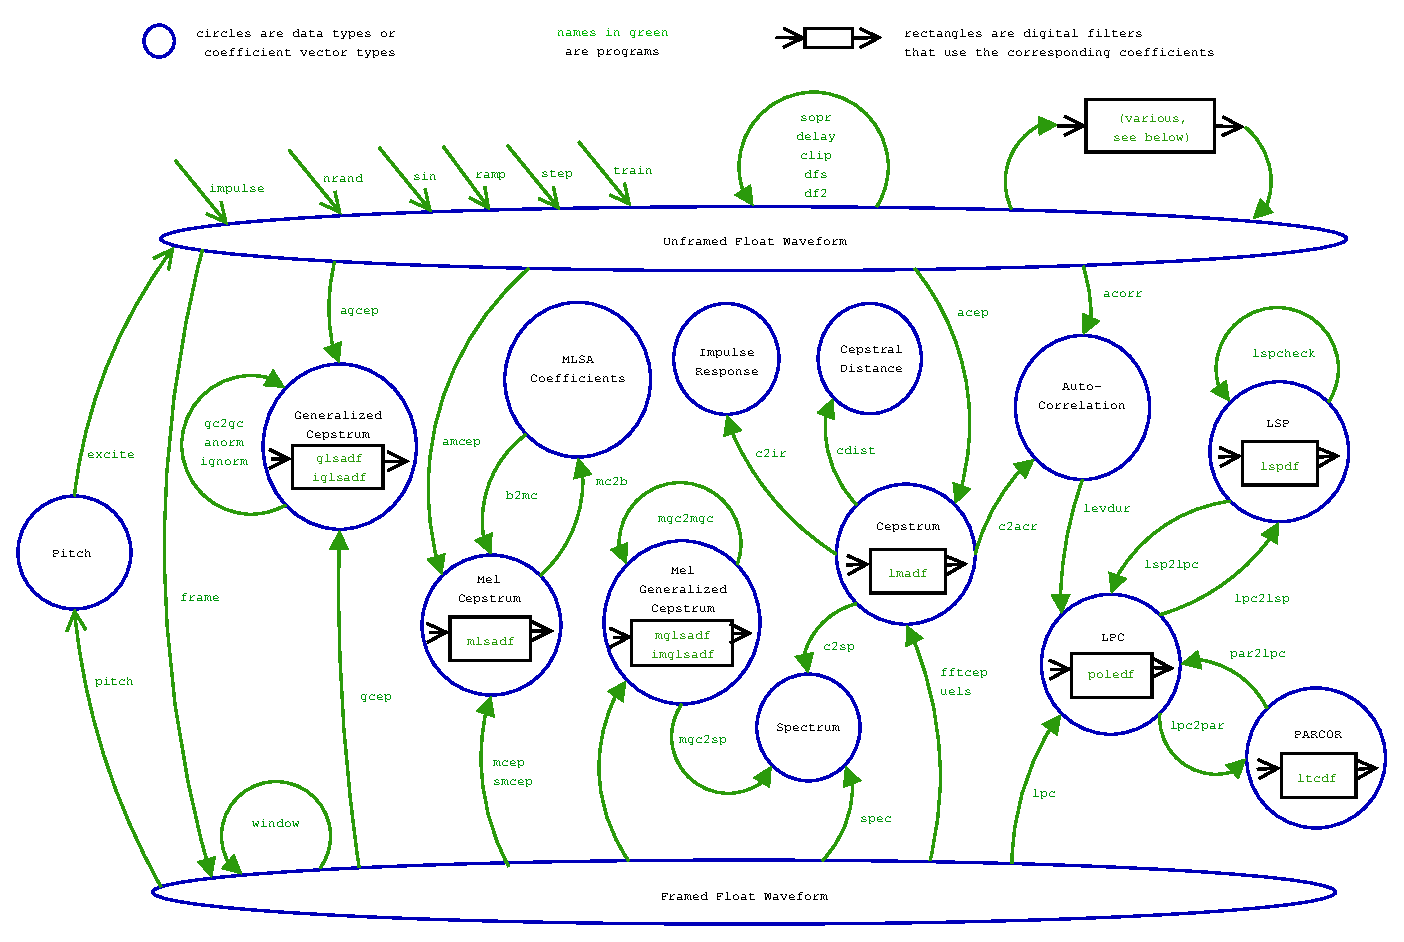
\includegraphics[width=16.5cm]{fig/sptk_sigproc.eps} 


\backmatter

\cleardoublepage
\printindex

\end{document}
